% \documentclass[11pt,a4paper]{report}
\documentclass[draft,11pt,a4paper]{report}

%% packages
\usepackage{a4wide}
\usepackage{amsmath,amssymb,amsthm}
\usepackage{booktabs}
\usepackage[czech]{babel}
\usepackage{enumerate}
\usepackage{forest}
\usepackage{multicol}
\usepackage{tcolorbox}
\usepackage{tikz}
    \usetikzlibrary{arrows.meta}
\usepackage[unicode]{hyperref}
\usepackage[utf8]{inputenc}
\usepackage{xfrac}


%% theorems
\theoremstyle{plain}
    \newtheorem{theorem}{Věta}[section]
    \newtheorem{proposition}[theorem]{Tvrzení}
    \newtheorem{corollary}[theorem]{Důsledek}
    \newtheorem{lemma}[theorem]{Lemma}
    \newtheorem{observation}[theorem]{Pozorování}
\theoremstyle{definition}
    \newtheorem{definition}[theorem]{Definice}
    \newtheorem*{algorithm}{Algoritmus}
\theoremstyle{remark}
    \newtheorem{remark}[theorem]{Poznámka}
    \newtheorem{example}[theorem]{Příklad}
    \newtheorem{exercise}{Cvičení}[chapter]
    \newtheorem*{solution}{Řešení}

%% macros and definitions
% \DeclareMathOperator{\AFm}{AFm}
\DeclareMathOperator{\Conseq}{Csq}
\DeclareMathOperator{\Fm}{Fm}
\DeclareMathOperator{\M}{M}
\DeclareMathOperator{\Term}{Term}
\DeclareMathOperator{\Tree}{Tree}
\DeclareMathOperator{\Thm}{Thm}
\DeclareMathOperator{\Var}{Var}
\DeclareMathOperator{\VF}{VF}

\newcommand{\A}{\structure{A}}
\newcommand{\B}{\structure{B}}
\newcommand{\disjointunion}{\mathbin{\dot{\sqcup}}}
\newcommand{\F}{\ensuremath{\mathrm{F}}}
\newcommand{\landsymb}{{\land}}
\newcommand{\lbin}{\mathbin{\square}}
\newcommand{\lbinsymb}{{\lbin}}
\newcommand{\liff}{\mathbin{\leftrightarrow}}
\newcommand{\liffsymb}{{\liff}}
\newcommand{\limplies}{\mathbin{\rightarrow}}
\newcommand{\limpliessymb}{{\limplies}}
\newcommand{\lorsymb}{{\lor}}
\newcommand{\proves}{\vdash}
\newcommand{\structure}[1]{\mathcal{#1}}
\newcommand{\todo}{[TODO]}
\newcommand{\T}{\ensuremath{\mathrm{T}}}
\newcommand{\union}{\mathbin{\cup}}

\begin{document}

% \input{chapters/current.tex}

% \title{NAIL062 Výroková a predikátová logika: \\ zápisky z přednášky}
\author{Jakub Bulín\footnote{KTIML MFF UK, \href{mailto://jakub.bulin@mff.cuni.cz}{jakub.bulin@mff.cuni.cz}}}
\date{Zimní semestr 2022, verze 0.1}
\maketitle

Přednáška je postavena na učebnici \emph{A. Nerode, R. Shore: Logic for Applications}~\cite{nerode_logic_2012}, některé části jsou z knihy \emph{M. Ben-ari: Mathematical Logic for Computer Science}~\cite{ben-ari_mathematical_2012}. Struktura kurzu i převážná většina obsahu jsou převzaty z přednášek Petra Gregora z předchozích let~\cite{gregor_vyrokova_nodate} (místy i doslovně, zejména v předběžných verzích jednotlivých sekcí), viz také anglická skripta Martina Piláta~\cite{pilat_lecture_nodate}. Najdete-li překlepy nebo jiné chyby, případně těžko srozumitelné části, prosím, napište mi.

\tableofcontents
% \chapter{Úvod do logiky}

%Úvod do logiky, syntaxe a sémantika výrokové logiky

Slovo \emph{logika} se používá ve dvou významech:
\begin{itemize}
    \item soubor principů, které jsou základem uspořádání prvků nějakého systému (např.\ počítačového programu, elektronického zařízení, komunikačního protokolu)
    \item uvažování prováděné podle striktních pravidel zachovávajících platnost
\end{itemize}
V informatice se tyto dva významy setkávají: nejprve formálně popíšeme daný systém, a poté o něm \emph{formálně uvažujeme} (v praktických aplikacích automaticky), tj.\ odvozujeme platné \emph{inference} o systému, za použití nějakého \emph{(formálního) dokazovacího systému}.

Mezi praktické aplikace logiky v informatice patří například software verification, logic programming, SAT solving, automated reasoning, nebo knowledge-based representation. Kromě toho je logika (ve větší míře než matematika) základním nástrojem pro popis teoretické informatiky. %Více o aplikacích logiky najdete v příloze~\ref{appendix:applications}; v příloze~\ref{appendix:history} je shrnuta historie logiky.



\section{Výroková logika}

Nyní si ukážeme logiku v akci na dvou příkladech ze života (hledače pokladů, a teoretického informatika):


\subsection{Příklad: Hledání pokladu}

\begin{tcolorbox}
\begin{example}
Při hledání pokladu v dračí sluji jsme narazili na rozcestí dvou chodeb. Víme, že na konci každé chodby je buď poklad, nebo drak, ale ne obojí. Trpaslík, kterého jsme na rozcestí potkali, nám řekl, že: ``Alespoň jedna z těch dvou chodeb vede k pokladu'', a po dalším naléhání (a menším úplatku), ještě řekl, že ``První chodba vede k drakovi.'' Je známo, že trpaslíci, které člověk potká v dračí sluji, buď vždy mluví pravdu, nebo vždy lžou. Kterou cestou se máme vydat?
\end{example}
\end{tcolorbox}

\subsection{Formalizace ve výrokové logice}

Začneme tím, že situaci a naše znalosti formalizujeme ve výrokové logice. \emph{Výrok} je tvrzení, kterému můžeme přiřadit pravdivostní hodnotu: \emph{pravdivý} (\emph{True}, 1), nebo \emph{lživý} (\emph{False}, 0). Některé výroky lze vyjádřit pomocí jednodušších výroků a logických spojek, např.  ``(Trpaslík lže,) \emph{právě když} (druhá chodba vede k drakovi.)'' nebo ``(První chodba vede k pokladu) \emph{nebo} (první chodba vede k drakovi.)'' Pokud výrok takto rozložit nelze, říká se mu \emph{prvovýrok}, \emph{atomický výrok}, nebo \emph{výroková proměnná}.

Popíšeme tedy celou situaci pomocí \emph{výrokových proměnných}. Můžeme si je také představit jako jednoduché zjišťovací (ano/ne) otázky, na které musíme znát odpověď, abychom věděli vše o dané situaci. Jako naše výrokové proměnné zvolme ``Poklad je v první chodbě.'' (označme \(p_1\)), a ``Poklad je v druhé chodbě.'' (\(p_2\)). V úvahu přichází i jiné výrokové proměnné, např. ``V první chodbě je drak.'' (\(d_1\)) nebo ``Trpaslík mluví pravdu.'' (\(t\)). Ty lze ale vyjádřit pomocí \( \{p_1,p_2\} \), např.\ platí \(t\), právě když neplatí \(p_1\). Tj.\ známe-li pravdivostní hodnoty \(p_1,p_2\), pravdivostní hodnoty \(d_1,t\) jsou jednoznačně určené. A menší počet výrokových proměnných znamená menší prohledávací prostor.

Vyjádříme tedy všechny naše znalosti jako (\emph{složené}) výroky a zapíšeme je ve formálním zápisu v \emph{jazyce} výrokové logiky nad množinou prvovýroků \( \mathbb P=\{p_1,p_2\} \), za použití symbolů reprezentujících logické spojky \( \neg \) (``neplatí X'', \emph{negace}), \( \landsymb \) (``X a Y'', \emph{konjunkce}), \( \lorsymb \) (``X nebo Y'', \emph{disjunkce}), \( \limpliessymb \) (``pokud X, potom Y'', \emph{implikace}), \( \liffsymb \) (``X, právě když Y'', \emph{ekvivalence}) a závorek (,). Zde je dobré zmínit, že disjunkce není exkluzivní, tj. ``X nebo Y'' platí i pokud platí jak X tak Y, a  implikace je čistě logická: ``pokud X, potom Y'' platí kdykoliv neplatí X nebo platí Y.

Informace o tom, že v chodbě je poklad nebo drak, ale ne obojí, už je zakódovaná v naší volbě výrokových proměnných: přítomnost draka je totéž co absence pokladu. Tvrzení trpaslíka, že ``První chodba vede k drakovi.'' tedy vyjádříme jako ``Neplatí, že poklad je v první chodbě.'', formálně \(\neg p_1\). Tvrzení, že ``Alespoň jedna z těch dvou chodeb vede k pokladu.'' vyjádříme jako ``Poklad je v první chodbě nebo poklad je v druhé chodbě.'', formálně \( p_1 \lor p_2\). Informaci, že trpaslíci buď vždy mluví pravdu, nebo vždy lžou, si přeložíme tak, že buď platí oba naše výroky, nebo platí negace obou našich výroků, formálně:
\[
    (\neg p_1 \land (p_1 \lor p_2)) \lor (\neg (\neg p_1) \land \neg (p_1 \lor p_2))
\]
Označme tento výrok jako \( \varphi \) (od slova ``formule'', výrokům se někdy také říká \emph{výrokové formule}). V našem příkladě lze všechny informace vyjádřit jediným výrokem, v praxi ale často potřebujeme výroků více, někdy i nekonečně mnoho (například pokud chceme popsat výpočet nějakého programu a nevíme apriori kolik kroků bude mít), potom popíšeme situaci pomocí množiny výroků, tzv. \emph{teorie}, zde \( T=\{ \varphi \} \). Výrokům z \( T \) říkáme také \emph{axiomy} teorie~\( T \)\footnote{Terminologie v logice často pochází z jejích aplikace v matematice.}.
%\footnote{Terminologie v logice často pochází z jejích aplikace v matematice, viz příloha~\ref{appendix:history} o historii logiky.}.

\subsection{Modely a důsledky}

Jsou naše informace dostačující k určení, zda je v některé z chodeb poklad? Jinými slovy, ptáme se, zda je jeden z výroků \( p_1, p_2 \) logickým \emph{důsledkem} výroku \( \varphi \), resp.\ teorie \( T \). Co to znamená?

Představme si, že existuje více různých ``světů'' lišících se v tom, co je na konci první a na konci druhé chodby. Například, v jednom ze světů je na konci první chodby poklad a na konci druhé chodby drak. Tento svět můžeme popsat pomocí pravdivostního ohodnocení výrokových proměnných: \( p_1=1, p_2=0 \). Takovému ohodnocení říkáme \emph{model} jazyka \( \mathbb P=\{p_1,p_2\} \) a zapisujeme ho zkráceně jako \( v = (1,0) \) (\(v\) od slova ``valuation''). Celkem tedy máme čtyři různé světy, popsané \emph{modely jazyka}
\[
    \M_\mathbb P=\{(0,0),(0,1),(1,0),(1,1)\}.
\]

Je svět popsaný modelem \( v = (1,0) \) konzistentní s informacemi, které máme, tj. \emph{platí} v něm výrok \( \varphi \), resp.\ teorie \( T \)? Pravdivostní hodnotu (složeného) výroku \( \varphi \) v modelu \(v\), označme ji \( v(\varphi) \), můžeme snadno zjistit: Víme, že \( v(p_1) = 1 \) a \( v(p_2) = 0 \), takže \( v(\neg p_1) = 0 \), a také \( v(\neg p_1 \land (p_1 \lor p_2))=0 \) (jde o konjunkci dvou výroků, a první z konjunktů je v modelu \( v \) nepravdivý). Podobně \( v(p_1 \lor p_2)=1 \) (neboť \( v(p_1) = 1 \)), takže \( v(\neg(p_1 \lor p_2))=0 \), a \( v(\neg (\neg p_1) \land \neg (p_1 \lor p_2))=0 \). Výrok \( \varphi \) je disjunkcí dvou výroků, z nichž ani jeden v modelu \(v\) neplatí, tedy \( v(\varphi)=0 \).  

Bystrý čtenář jistě vidí stromovou strukturu výroku \( \varphi \) a postupné vyhodnocování \( v(\varphi) \) od listů směrem ke kořeni. Formální definice představíme v příští kapitole.

Podobně určíme pravdivostní hodnoty výroku \( \varphi \) v ostatních modelech. Zjistíme, že množina \emph{modelů výroku} \( \varphi \) (resp.\ \emph{modelů teorie} \( T \)), tj.\ množina všech modelů jazyka, ve kterých platí \( \varphi \) (resp.\ všechny výroky z teorie \( T \)), je
\[	
    \M_\mathbb P(\varphi)=\M_\mathbb P(T)=\{(0,1)\}.
\]
Vidíme, že naše informace jednoznačně určují model \( (0,1) \), tedy svět, ve kterém je v první chodbě drak a ve druhé poklad. Obecně modelů může být více, stačí nám vědět, že v každém modelu \( \varphi \), resp.{\ }\(T \), platí výrok \( p_2 \), tedy že \( p_2 \) je \emph{důsledkem} teorie \( T \); také říkáme, že \( p_2 \) \emph{platí} v teorii \( T \).

\subsection{Dokazovací systémy}

Postup, který jsme zvolili, je velmi neefektivní. Máme-li \( n \) výrokových proměnných\footnote{V praxi máme běžně tisíce proměnných.}, existuje~\( 2^n \) modelů jazyka a není prakticky možné ověřovat platnost teorie v každém z nich. Na řadu přichází tzv.\ \emph{dokazovací systémy}. V daném dokazovacím systému je \emph{důkaz} výroku~\( \psi \) z teorie \(T\) přesně, formálně definovaný syntaktický objekt, který v sobě zahrnuje snadno (mechanicky) ověřitelný ``důkaz'' (důvod), proč \( \psi \) platí v \(T\), a který můžeme hledat (pomocí počítače) čistě na základě struktury výroku \( \psi \) a axiomů teorie \(T\) (``syntaxe''), tj.\ aniž bychom se museli zabývat modely (``sémantikou'').

Po důkazovém systému chceme dvě vlastnosti: 
\begin{itemize}
    \item \emph{korektnost}, tj.\ pokud máme důkaz \( \psi \) z \(T\), potom \( \psi \) platí v \(T\), a
    \item \emph{úplnost}, tj.\ pokud \( \psi \) platí v \(T\), potom existuje důkaz \( \psi \) z \(T\),
\end{itemize}
přičemž korektnost je nutností (bez ní nemá smysl důkazy hledat), a úplnost je dobrá vlastnost, ale efektivní důkazový systém může být užitečný, i pokud v něm nelze dokázat vše, co platí.

Zde stručně nastíníme dva důkazové systémy: \emph{metodu analytického tabla} a \emph{rezoluční metodu}. Později budou představeny formálně, a u obou si dokážeme i jejich korektnost a úplnost. Oba tyto důkazové systémy jsou založeny na \emph{důkazu sporem}, tj.\ předpokládají platnost axiomů z \(T\) a negace výroku \( \psi \), a snaží se dojít ke sporu.

\subsection{Tablo metoda}

V metodě analytického tabla je důkazem \emph{tablo}: strom jehož vrcholy jsou označkované předpoklady o platnosti výroků. Podívejme se na příklad tabla na obrázku~\ref{figure:tableaux-proof-example}. 

\begin{figure}
    \centering
    \begin{forest}
    [False \( p_2 \)
        [True \( (\neg p_1 \land (p_1 \lor p_2)) \lor (\neg (\neg p_1) \land \neg (p_1 \lor p_2)) \) 
            [True \( \neg p_1 \land (p_1 \lor p_2) \)
                [True \( \neg p_1 \)
                    [True \( p_1 \lor p_2 \)
                        [False \( p_1 \)
                            [True \( p_1 \), tikz={\node[fit to=tree,label=below:\emph{fail}] {};}
                            ]
                            [True \( p_2 \), tikz={\node[fit to=tree,label=below:\emph{fail}] {};}
                            ]
                        ]
                    ]
                ]
            ]
            [True \( \neg (\neg p_1) \land \neg (p_1 \lor p_2) \)
                [True \( \neg (\neg p_1) \)
                    [True \(\neg (p_1 \lor p_2) \)
                        [False \( (\neg p_1) \)
                            [True \( p_1 \)
                                [False \(p_1 \lor p_2 \)
                                    [False \(p_1\)
                                        [False \(p_2\), tikz={\node[fit to=tree,label=below:\emph{fail}] {};}
                                        ]
                                    ]
                                ]
                            ]
                        ]
                    ]
                ]
            ]
        ]
    ]
    \end{forest}

\caption{Tablo důkaz výroku \( p_2 \) z teorie \(T\)}\label{figure:tableaux-proof-example}
\end{figure}

Začneme předpokladem, že neplatí výrok \(p_2\) (neboť dokazujeme sporem). Poté připojíme platnost všech axiomů teorie \(T\) (v našem případě je jen jeden: výrok \( \varphi \) sestrojený výše). Dále budujeme tablo tak, že zjednodušujeme výroky v předpokladech, a to podle jistých pravidel, která zaručují následující invariant: 

\begin{tcolorbox}
\emph{Každý model teorie \(T\), ve kterém neplatí \(p_2\), se musí \emph{shodovat} s některou z větví tabla (tj.\ splňovat všechny předpoklady na dané větvi).} 
\end{tcolorbox}

Výrok \( \varphi \) je disjunkcí dvou výroků, \( \varphi = \varphi_1 \lor \varphi_2 \). Pokud tedy platí v nějakém modelu, potom buď v tomto modelu platí \( \varphi_1 \), nebo v něm platí \( \varphi_2 \). Rozvětvíme strom podle těchto dvou možností. V dalším kroku máme předpoklad o pravdivosti výroku \( \neg p_1 \land (p_1 \lor p_2) \). V tom případě musí platit jak \( \neg p_1 \), tak \( p_1 \lor p_2 \), připojíme tedy na konec větve oba tyto předpoklady. Pravdivost \( \neg p_1 \) znamená lživost \( p_1 \), a tak dále.

Takto postupujeme, dokud je možné výroky v předpokladech zjednodušit, tj.\ dokud to nejsou jen výrokové proměnné. Pokud na jedné větvi najdeme dvojici opačných předpokladů o nějakém výroku \( \psi \), tj.\ že platí, a zároveň že neplatí, víme, že se s touto větví nemůže shodovat žádný model. Takové větvi říkáme \emph{sporná}.  Protože dokazujeme sporem, důkaz je takové tablo, ve kterém je každá větev sporná. Tím je zaručeno, že neexistuje model \(T\), ve kterém neplatí \(p_2\). Z toho plyne, že \(p_2\) platí v každém modelu \(T\), neboli je to důsledek \(T\), což jsme chtěli dokázat.

Zatím se spokojíme s pochopením základní myšlenky této metody, detaily představíme v budoucí kapitole.
 
\subsection{Rezoluční metoda}

Není těžké naprogramovat systematické hledání tablo důkazu. V praxi se ale používá jiný důkazový systém, který má mnohem jednodušší a efektivnější implementaci: tzv.\ \emph{rezoluční metoda}. Tato metoda pochází z roku 1965, a je základem většiny \emph{systémů automatického dokazování}, \emph{SAT solverů}, nebo třeba interpreterů jazyka Prolog (o kterém si budeme povídat později).

Rezoluční metoda je založena na faktu, že každý výrok lze ekvivalentně vyjádřit ve speciálním tvaru, v tzv.\ \emph{konjunktivní normální formě (CNF)}. \emph{Literál} je výroková proměnná \(p\) nebo její negace \(\neg p\) (tj.\ literály jsou výroky, které jen určují hodnotu jedné výrokové proměnné). Disjunkci několika literálů, např. \( p \lor \neg q\lor \neg r\), říkáme \emph{klauzule}. A výrok je v CNF, pokud je konjunkcí klauzulí. Ke každému výroku \( \psi \) existuje \emph{ekvivalentní} výrok \( \psi' \) v {CNF}. Ekvivalentní znamená mající stejný význam (stejné modely), píšeme \( \psi \sim \psi' \). Později si ukážeme dvě metody převodu do CNF, nyní jen na našem příkladě: ve výroku
\[
    (\neg p_1 \land (p_1 \lor p_2)) \lor (\neg (\neg p_1) \land \neg (p_1 \lor p_2))
\]
nejprve nahradíme \( \neg (\neg p_1) \sim p_1 \) a \( \neg (p_1 \lor p_2) \sim (\neg p_1 \land \neg p_2) \):
\[
    (\neg p_1 \land (p_1 \lor p_2)) \lor (p_1 \land \neg p_1 \land \neg p_2)
\]
a dále opakovaně použijeme \emph{distributivitu} \( \lorsymb \) vůči \( \landsymb \) (představte si, že \( \lorsymb \) je operace násobení a \( \landsymb \) je operace sčítání):
\[
    (\neg p_1 \lor p_1) \land (\neg p_1 \lor \neg p_1) \land (\neg p_1 \lor \neg p_2) \land (p_1 \lor p_2 \lor p_1) \land (p_1 \lor p_2 \lor \neg p_1) \land (p_1 \lor p_2 \lor \neg p_2)
\]
Tento výrok už je v CNF, ale dále ho zjednodušíme: vynecháme z klauzulí duplicitní literály, a uvědomíme si, že obsahuje-li klauzule dvojici opačných literálů \( p, \neg p \), je to \emph{tautologie} (platí v každém modelu) a proto ji můžeme odstranit. Dostáváme CNF výrok
\[
    \neg p_1 \land (\neg p_1 \lor \neg p_2) \land (p_1 \lor p_2)
\]
který je ekvivalentní původnímu výroku \( \phi \)
Protože chceme dokázat \(p_2\) sporem, přidáme ještě klauzuli \(\neg p_2\):
\[
    \neg p_1 \land (\neg p_1 \lor \neg p_2) \land (p_1 \lor p_2) \land \neg p_2
\]
Výrok \(p_2\) platí v teorii \(T\), právě když je tento CNF výrok \emph{nesplnitelný} (nemá žádný model). Výroky v CNF budeme zapisovat také v \emph{množinové reprezentaci}\footnote{V praktické implementaci bychom mohli použít seznam klauzulí, kde každá klauzule je seznam (unikátních) literálů v nějakém zvoleném uspořádání. Představte si opět tisíce výrokových proměnných a klauzulí.}:
\[
    \left \{ \{\neg p_1\},\{\neg p_1,\neg p_2\},\{p_1, p_2\},\{\neg p_2\} \right \}
\]
\emph{Rezoluční pravidlo} říká, že pokud máme dvojici klauzulí, z nichž jedna obsahuje literál \(p\) a druhá opačný literál \(\neg p\), potom z nich logicky plyne také jejich\ \emph{rezolventa}: klauzule vzniklá odstraněním literálu \(p\) z první a \(\neg p\) z druhé klauzule a sjednocením zbylých literálů. Například, z \( p \lor \neg q\lor \neg r\) a \( \neg p \lor \neg q \lor s\) můžeme odvodit rezolventu \( \neg q \lor \neg r \lor s\). \emph{Rezoluční zamítnutí} formule v CNF je potom posloupnost klauzulí, která končí \emph{prázdnou klauzulí \( \square \)} (znamenající spor) a kde každá klauzule je buď z dané formule, nebo je rezolventou nějakých dvou předchozích klauzulí. V našem případě:
\[
    \{\neg p_1\},\{p_1, p_2\},\{p_2\},\{\neg p_2\},\square
\]
Třetí klauzule je rezolventou první a druhé, pátá je rezolventou třetí a čtvrté. Rezoluci lze také přirozeně znázornit pomocí \emph{rezolučního stromu}, kde listy jsou klauzule z dané formule, a vnitřní vrcholy jsou rezolventy svých potomků:

\begin{center}
\begin{forest}
for tree={grow=north}
[\( \square \)
    [\( \{\neg p_2\} \)]
    [\( \{p_2\} \)
    [{\( \{p_1, p_2\} \)}]
    [\( \{\neg p_1\} \)]
    ]
]
\end{forest}
\end{center}

Pokud by formule měla model, musely by v něm platit její klauzule, tedy i postupně všechny rezolventy v posloupnosti, a nakonec prázdná klauzule. Ta ale neplatí v žádném modelu. Máme tedy důkaz sporem a víme, že ve druhé chodbě najdeme poklad.


\subsection{Příklad: Barvení grafů}\label{subsection:example-graph-coloring}

Ve druhém příkladu se trochu přiblížíme aplikacím. Na rozdíl od logických hádanek ve formě slovních úloh, různé varianty problému barvení grafů se objevují v rozmanitých úlohách z praxe, od rozvrhovacích problémů přes návrh fyzických a síťových systémů po zpracování obrazu.

\begin{tcolorbox}
\begin{example}\label{example:graph-coloring-intro}
Najděte vrcholové obarvení následujícího grafu třemi barvami, tj.\ přiřaďte vrcholům barvy R, G, B tak, aby žádná hrana nebyla monochromatická.
\begin{center}
\begin{tikzpicture}[every node/.style={circle,fill=blue!10,draw,minimum size=0.5cm,node distance=1.5cm}]
\node (1) {$1$};
\node[right of=1] (2) {$2$};
\node[below of=2] (3) {$3$};
\node[left of=3] (4) {$4$};
\path[draw] (1) -- (2) -- (3) -- (4) -- (1) -- (3);
\end{tikzpicture}
\end{center}
\end{example}
\end{tcolorbox}

Graf si reprezentujeme jako množinu vrcholů a množinu hran, kde každá hrana je dvojice vrcholů. Lépe se nám bude pracovat s uspořádanými dvojicemi, zvolíme tedy (libovolnou) orientaci hran.
\[
\structure G = \langle V; E \rangle = \langle \{1,2,3,4\}; \{(1,2),(1,3),(1,4),(2,3),(3,4)\} \rangle
\]



Začneme opět formalizací ve výrokové logice. Označme si množinu barev jako \( C=\{R,G,B\} \).  Přirozená volba výrokových proměnných je ``vrchol \(v\) má barvu \(c\)'', označme \(p_v^c\), pro každý vrchol \(v \in V\) a každou barvu \(c\in C\). Naše (uspořádaná) množina výrokových proměnných má 12 prvků:
\[
\mathbb P=\{p_v^c\mid c\in C,v\in V\}=\{p_1^R,p_1^G,p_1^B,p_2^R,p_2^G,p_2^B,p_3^R,p_3^G,p_3^B,p_4^R,p_4^G,p_4^B\}
\]
Máme celkem \( |\M_\mathbb P|=2^{12}=4096 \) modelů jazyka (reprezentovaných 12-dimenzionálními 0--1 vektory). Většinu z nich nelze interpretovat jako obarvení grafu. Například \( v=(1,1,0,0,\dots,0) \) říká, že vrchol 1 je obarvený červeně, a také zeleně. Začneme tedy teorií vyjadřující, že každý vrchol má nejvýše jednu barvu. Existuje více způsobů, jak to můžeme vyjádřit. My řekneme pro každý vrchol, že nesmí mít (alespoň) jednu z každé dvojice barev. Tím dostaneme teorii v {CNF}:

\begin{align*}
T_1 = \{ 
&(\neg p_1^R \lor \neg p_1^G) \land (\neg p_1^R \lor \neg p_1^B) \land (\neg p_1^G \lor \neg p_1^B),\\
&(\neg p_2^R \lor \neg p_2^G) \land (\neg p_2^R \lor \neg p_2^B) \land (\neg p_2^G \lor \neg p_2^B),\\
&(\neg p_3^R \lor \neg p_3^G) \land (\neg p_3^R \lor \neg p_3^B) \land (\neg p_3^G \lor \neg p_3^B),\\
&(\neg p_4^R \lor \neg p_4^G) \land (\neg p_4^R \lor \neg p_4^B) \land (\neg p_4^G \lor \neg p_4^B)\} \\
    = \{ &(\neg p_v^R \lor \neg p_v^G) \land (\neg p_v^R \lor \neg p_v^B) \land (\neg p_v^G \lor \neg p_v^B) \mid v \in V \} 
\end{align*}
Teorii \(T_1\) bychom mohli říkat teorie částečných vrcholových obarvení grafu \(\structure G\). Teorie \(T_1\) má \(|\M_\mathbb P(T_1)|= 4^4=2^8=256\) modelů. (Proč?) Pokud chceme úplná obarvení, přidáme podmínku, že každý vrchol má alespoň jednu barvu.\footnote{Symbol \(\bigvee \) používáme podobně jako symboly \(\sum \) pro součet a \(\prod \) pro součin: ke zjednodušení zápisu výroku, který je ve formě disjunkce. Např.\ pokud \(v=1\), potom \( \bigvee_{c\in C} p_v^c \) reprezentuje výrok \( p_1^R \lor p_1^G \lor p_1^B \). Analogicky \(\bigwedge \) pro konjunkci.}

\begin{align*}
T_2 &= T_1\cup \{p_1^R \lor p_1^G \lor p_1^B, p_2^R \lor p_2^G \lor p_2^B, p_3^R \lor p_3^G \lor p_3^B, p_4^R \lor p_4^G \lor p_4^B\} \\
    &= T_1\cup \{ p_v^R \lor p_v^G \lor p_v^B \mid v \in V \} \\
    &= T_1\cup \{\bigvee_{c\in C} p_v^c \mid v \in V \}  
\end{align*}

Teorie \( T_2 \) má \(3^4=81\) modelů. Jde o \emph{extenzi} teorie \( T_1 \), neboť každý důsledek teorie \( T_1 \) platí i v teorii \( T_2 \). Platí dokonce, že \( \M_\mathbb P(T_2)\subseteq\M_\mathbb P(T_1) \).\footnote{Zde vidíme typickou ukázku antimonotónního vztahu tzv.\ Galoisovy korespondence: čím více vlastností (výroků) požadujeme, tím méně objektů (modelů) splňuje tyto vlastnosti.} Zbývá přidat podmínku zakazující monochromatické hrany. Pro každou hranu a každou barvu specifikujeme, že alespoň jeden z vrcholů hrany nesmí mít danou barvu. Zde pro názornost naposledy napíšeme úplný seznam výroků, nadále budeme využívat zkráceného zápisu.
\begin{align*}
    T_3 = T_2\cup \{ & (\neg p_1^R \lor \neg p_2^R) \land (\neg p_1^G \lor \neg p_2^G) \land (\neg p_1^B \lor \neg p_2^B),\\
    & (\neg p_1^R \lor \neg p_3^R) \land (\neg p_1^G \lor \neg p_3^G) \land (\neg p_1^B \lor \neg p_3^B),\\
    & (\neg p_1^R \lor \neg p_4^R) \land (\neg p_1^G \lor \neg p_4^G) \land (\neg p_1^B \lor \neg p_4^B),\\
    & (\neg p_2^R \lor \neg p_3^R) \land (\neg p_2^G \lor \neg p_3^G) \land (\neg p_2^B \lor \neg p_3^B),\\
    & (\neg p_3^R \lor \neg p_4^R) \land (\neg p_3^G \lor \neg p_4^G) \land (\neg p_3^B \lor \neg p_4^B)\} \\  
= T_2\cup \{ &\bigwedge_{c\in C} 
(\neg p_u^c \lor \neg p_v^c) \mid (u,v) \in E \}
\end{align*}
Výsledná teorie \( T_3 \) je \emph{splnitelná} (má model), právě když graf \( \structure{G} \) je 3-obarvitelný. Má 6 modelů jednoznačně odpovídajících 3-obarvení grafu \( \structure G \). Model \( v = (1,0,0,0,1,0,0,0,1,0,1,0) \) odpovídá následujícímu obarvení, ostatní obarvení získáme permutací barev.
\begin{center}
\begin{tikzpicture}[every node/.style={circle,fill=blue!10,draw,minimum size=0.5cm,node distance=1.5cm}]
\node[fill=red] (1) {$1$};
\node[fill=green,right of=1] (2) {$2$};
\node[fill=blue,below of=2] (3) {$3$};
\node[fill=green,left of=3] (4) {$4$};
\path[draw] (1) -- (2) -- (3) -- (4) -- (1) -- (3);
\end{tikzpicture}
\end{center}

Jakmile máme teorii \(T_3\) formalizující 3-obarvení grafu \( \structure{G} \), můžeme snadno řešit související otázky, například najít všechna obarvení, ve kterých je vrchol 1 modrý a vrchol 2 zelený: odpovídají modelům teorie \( T_3 \cup \{ p_1^B, p_2^G\} \). Nebo můžeme dokázat, že vrcholy 2 a 4 musejí být obarveny stejnou barvou. Můžeme použít tablo metodu: v kořeni tabla bude předpoklad
\[
\text{False  }(p_2^R \land p_4^R)\lor(p_2^G \land p_4^G)\lor(p_2^B \land p_4^B)
\]
Nebo můžeme najít rezoluční zamítnutí teorie vzniklé převedením axiomů teorie \( T_3 \) do CNF, a přidáním CNF ekvivalentu \emph{negace} výroku \( (p_2^R \land p_4^R)\lor(p_2^G \land p_4^G)\lor(p_2^B \land p_4^B) \)	(neboť jde o důkaz sporem, tedy pro spor předpokládáme, že \emph{nemají} stejnou barvu).



\section{Predikátová logika}

Nyní si velmi stručně a neformálně představíme \emph{predikátovou logiku}. Predikátová logika se zabývá vlastnostmi objektů a vztahy mezi objekty. Například:
\begin{quote}\it
    Všichni lidé jsou smrtelní.\\
    Sókratés je člověk.\\
    Sókratés je smrtelný.
\end{quote}
Ve skutečnosti výroková logika vznikla později (asi o století) než Aristotelova predikátová logika, a byla poté na dlouho převážně zapomenuta.


\subsection{Nevýhody formalizace ve výrokové logice}\label{subsection:disadvantages-of-propositional-logic}

Nevýhodou formalizace našeho problému ve výrokové logice je fakt, že výsledná teorie \( T_3 \) je poměrně velká, a navíc byla vytvořena ad hoc pro graf  \( \structure{G} \). Představme si, že potřebujeme graf \( \structure{G} \) změnit, například přidáním vrcholu 5 spojeného hranami s vrcholy 2 a 3:

\begin{center}
    \begin{tikzpicture}[every node/.style={circle,fill=blue!10,draw,minimum size=0.5cm,node distance=1.5cm}]
    \node (1) {$1$};
    \node[right of=1] (2) {$2$};
    \node[below of=2] (3) {$3$};
    \node[left of=3] (4) {$4$};
    \path[draw] (1) -- (2) -- (3) -- (4) -- (1) -- (3);
    \node[right of=3] (5) {$5$};
    \path[draw] (2) -- (5) -- (3);
    \end{tikzpicture}
\end{center}

Abychom byli schopni formalizovat nový problém, musíme přidat do našeho jazyka tři nové výrokové proměnné: \(\mathbb P'=\mathbb P \cup \{ p_5^R,p_5^G,p_5^B\} \), a vytvořit nové teorie \( T'_1, T'_2, T'_3 \) přidáním axiomů týkajících se vrcholu 5 a hran \( (2, 5), (3,5) \). Problémem je, že strukturu grafu \( \structure{G} \) a přirozené vlastnosti jako ``z vrcholu \(u\) vede hrana do vrcholu \(v\)'', nebo ``vrchol \(u\) je zelený'' jsme (`natvrdo', `nepřirozeně') zakódovali do 0--1 proměnných. Tento nedostatek odstraňuje \emph{predikátová logika}.

\subsection{Stručné představení predikátové logiky}

\emph{Modelem} v predikátové logice není 0--1 vektor, ale \emph{struktura}. Příkladem struktur jsou naše (orientované) grafy:
\begin{align*}
    &\structure G = \langle V^\structure G; E^\structure G \rangle = \langle \{1,2,3,4\}; \{(1,2),(1,3),(1,4),(2,3),(3,4)\} \rangle \\ 
    &\structure{G}' = \langle V^{\structure{G}'}; E^{\structure{G}'} \rangle = \langle \{1,2,3,4,5\}; \{(1,2),(1,3),(1,4),(2,3),(3,4),(2,5),(3,5)\} \rangle
\end{align*}
Oba grafy sestávají z množiny vrcholů, a z binární relace na této množině. Jde o struktury v \emph{jazyce teorie grafů} \( \mathcal L=\langle E \rangle \), kde \(E\) je binární \emph{relační symbol}. \emph{Jazyk} predikátové logiky specifikuje jaké relace (kolik a jakých arit --- unární, binární, ternární, atd.) mají struktury mít, a jaké symboly pro ně budeme používat. Kromě toho používáme symbol rovnosti \(=\) a struktury mohou obsahovat také funkce a konstanty (jako například funkce \( +,-,\cdot \) a konstanty $0,1$ v \emph{tělese} reálných čísel), ty si ale necháme na později.

Predikátová logika používá tytéž logické spojky jako výroková logika, ale základním stavebním kamenem \emph{predikátových formulí} nejsou výrokové proměnné, nýbrž tzv.\ \emph{atomické formule}, například: \( E(x,y) \) představuje tvrzení, že v grafu vede hrana z vrcholu \(x\) do vrcholu \(y\). Zde \(x,y\) jsou \emph{proměnné} reprezentující vrcholy daného grafu. Kromě toho ve formulích můžeme používat \emph{kvantifikátory}: \( (\forall x) \) ``pro všechny vrcholy \(x\)'' a \( (\exists y) \) ``existuje vrchol \(y\)''.\footnote{Kvantifikátory si můžeme představit jako ``konjunkci'' resp.\ ``disjunkci'' přes všechny vrcholy grafu.} 

Nyní můžeme formalizovat tvrzení, která dávají smysl pro libovolný graf. Například: 
\begin{itemize}
    \item ``V grafu nejsou smyčky'': \[ (\forall x)(\neg E(x,x)) \] 
    \item ``Existuje vrchol výstupního stupně 1'': \[ (\exists x)(\exists y)(E(x,y) \land (\forall z)(E(x,z) \limplies y=z)) \] 
\end{itemize}
V daném grafu \(\structure{G}\) a při dosazení vrcholu \(u\) za proměnnou \(x\) a vrcholu \(v\) za proměnnou \(y\) vyhodnotíme \( E(x,y) \) jako True, právě když \( (u,v)\in E^{\structure{G}} \).


\subsection{Formalizace barvení grafů v predikátové logice}


Vraťme se zpět k barvení grafů. Přirozený způsob jak formalizovat náš problém 3-obarvitelnosti je v jazyce \( \mathcal L' =\langle E, R, G, B \rangle \), kde \(E\) je binární a \(R,G,B\) jsou unární relační symboly, tedy \(R(x)\) znamená ``vrchol \(x\) je červený''. Strukturou pro tento jazyk je (orientovaný) graf spolu s trojicí množin vrcholů, např.
\begin{align*}
\structure G_C &= \langle V^{\structure G_C}; E^{\structure G_C}, R^{\structure G_C}, G^{\structure G_C}, B^{\structure G_C} \rangle \\
&= \langle \{1,2,3,4\}; \{(1,2),(1,3),(1,4),(2,3),(3,4)\}, \{1\}, \{2,4\}, \{3\} \rangle    
\end{align*}
reprezentuje graf \( \structure{G} \) s validním obarvením z obrázku výše. Budeme říkat, že \( \structure{G}_C \) je \emph{expanze} \(\mathcal L\)-struktury \( \structure{G} \) do jazyka \( \mathcal L' \).

Podobně jako ve výrokové logice musíme nejprve zajistit, aby naše modely reprezentovaly obarvené grafy. Začneme požadavkem, aby každý vrchol byl obarven nejvýše jednou barvou:
\[
(\forall x)((\neg R(x) \lor \neg G(x)) \land (\neg R(x) \lor \neg B(x)) \land (\neg G(x) \lor \neg B(x)))
\]
Obarvení alespoň jednou barvou vyjádříme takto:
\[
(\forall x)(R(x) \lor G(x) \lor B(x))
\]
A hranovou podmínku formalizujeme pomocí predikátu \( E(x,y) \) například takto:
\[	
(\forall x)(\forall y)(E(x,y) \limplies ((\neg R(x) \lor \neg R(y)) \land (\neg G(x) \lor \neg G(y)) \land (\neg B(x) \lor \neg B(y))))
\]
Modely takto vzniklé teorie reprezentují orientované grafy s vrcholovým 3-obarvením. 


\section{Další druhy logických systémů}

Predikátové logice, kde proměnné reprezentují jednotlivé vrcholy, říkáme logika \emph{prvního řádu} (anglicky  \emph{first-order (FO) logic}). V logice \emph{druhého řádu} (anglicky \emph{second-order (SO) logic}) máme také proměnné reprezentující množiny vrcholů nebo i množiny \(n\)-tic vrcholů (tj.\ relace, funkce). Například tvrzení, že každá neprázdná zdola omezená podmnožina má infimum\footnote{Což platí v uspořádané množině reálných čísel, ale neplatí v racionálních číslech, např.\ \( \{x \mid x^2 > 2, x > 0\} \).}, můžeme formalizovat v logice druhého řádu takto:\footnote{I když je tato formule velmi složitá, pokuste se porozumět jednotlivým částem.}
\begin{align*}
&(\forall S)((\exists x)S(x) \land (\exists x)(\forall y)(S(y) \limplies x\leq y) \limplies  {}\\ 
&(\exists x)((\forall y)(S(y) \limplies x\leq y) \land (\forall z)((\forall y)(S(y) \limplies z\leq y)\limplies z\leq x)))
\end{align*}
V logice třetího řádu máme i proměnné reprezentující množiny množin (což je užitečné např.\ v topologii), atd.

Kromě výrokové a predikátové logiky existují i další typy logických systémů, například intuicionistická logika (která povoluje jen konstruktivní důkazy), temporální logiky (kde mluvíme o platnosti `vždy', `někdy v budoucnosti', `dokud' apod.), modální logiky (`je možné', `je nutné'), nebo fuzzy logiky (kde máme výroky `0.35 pravdivé'). Tyto logiky mají důležité aplikace v informatice, např.\ v umělé inteligenci (modální logiky pro uvažování autonomních agentů o svém okolí), v paralelním programování (temporální logiky), nebo v automatických pračkách (fuzzy logiky). %Více viz Příloha~\ref{appendix:other-logics}. 
V tomto kurzu se omezíme na výrokovou logiku a predikátovou logiku prvního řádu.


\section{O přednášce}

Přednášku lze rozdělit do třech částí. 

První část se zabývá výrokovou logikou. Nejprve představíme syntaxi a sémantiku, dále problém splnitelnosti CNF formulí (známý NP-úplný problém SAT) a jeho polynomiálně řešitelné fragmenty (2-SAT, Horn-SAT). Budeme pokračovat tablo metodu, u níž si dokážeme korektnost a úplnost, a také několik aplikací, například Větu u kompaktnosti. A na závěr představíme rezoluční metodu ve výrokové logice.

Ve druhé části představíme predikátovou logiku. Začneme opět syntaxí a sémantikou, ukážeme si jak lze adaptovat tablo metodu pro predikátovou logiku, a skončíme znovu rezoluční metodou. Kromě toho zmíníme několik praktických aplikací: databázové dotazy, logické programování (jazyk Prolog), a softwarovou verifikaci.

Třetí část je úvodem do teorie modelů, definovatelnosti, axiomatizovatelnosti, a algoritmické rozhodnutelnosti. Na závěr si představíme slavné Gödelovy věty o neúplnosti, které ukazují meze formální metody (formální dokazatelnosti v axiomatickém systému).



% \part{Výroková logika}

% \chapter{Syntaxe a sémantika výrokové logiky}

\emph{Syntaxe} je soubor formálních pravidel pro tvoření korektních vět sestávajících ze slov (v případě přirozených jazyků), nebo formálních výrazů sestávajících ze symbolů (např.\ příkazy v programovacím jazyce). Naproti tomu \emph{sémantika} popisuje význam takových výrazů. Vztah mezi syntaxí a sémantikou se prolíná celou logikou a je klíčem k jejímu pochopení.


\section{Syntaxe výrokové logiky}

Nejprve definujeme formální `nápisy', se kterými budeme v logice pracovat.


\subsection{Jazyk}

\emph{Jazyk} výrokové logiky je určený neprázdnou množinou \emph{výrokových proměnných} \( \mathbb P \) (také jim říkáme \emph{prvovýroky} nebo \emph{atomické výroky}). Tato množina může být konečná nebo i nekonečná, obvykle ale bude spočetná\footnote{To je důležité v mnoha aplikacích v informatice, nespočetné množiny se do počítače nevejdou.} (pokud neřekneme jinak), a bude mít dané uspořádání. Pro výrokové proměnné budeme obvykle používat označení \( p_i\) (od slova ``proposition''), ale pro lepší čitelnost, zejména je-li \( \mathbb P \) konečná, také \(p,q,r,\dots \) Například:
\begin{align*}
    \mathbb P_1 &= \{ p, q, r\}\\
    \mathbb P_2 &= \{ p_0, p_1, p_2, p_3, \ldots \} = \{ p_i \mid i \in \mathbb N \}
\end{align*}

Do jazyka patří kromě výrokových proměnných také \emph{logické symboly}: symboly pro logické spojky \( \neg,\landsymb,\lorsymb, \limpliessymb, \liffsymb \) a závorky \( (,) \). Budeme ale pro jednoduchost mluvit o ``jazyce~\( \mathbb P \)''.

\begin{remark}\label{remark:order-of-language}
Pokud budeme potřebovat formálněji vyjádřit uspořádání jazyka $\mathbb P$, představíme si ho jako bijekci $\iota\colon\{0,1,\dots,n-1\}\to \mathbb P$ (pro konečný, $n$-prvkový jazyk) resp.\ $\iota\colon\mathbb N\to \mathbb P$ (je-li $\mathbb P$ spočetně nekonečný). V našich příkladech $\iota_1(0)=p$, $\iota_1(1)=q$, $\iota_1(2)=r$, a $\iota_2(i)=p_i$ pro všechna $i\in\mathbb N$.\footnote{Množina přirozených čísel $\mathbb N$ obsahuje nulu, viz standard ISO 80000-2:2019.}
\end{remark}


\subsection{Výrok}

Základním stavebním kamenem výrokové logiky je \emph{výrok} neboli \emph{výroková formule}. Je to konečný řetězec sestavený z výrokových proměnných a logických symbolů podle jistých pravidel. Prvovýroky jsou výroky, a dále můžeme vytvářet výroky z jednodušších výroků a logických symbolů: například pro logickou spojku $\landsymb$ vypíšeme nejprve symbol `(', potom první výrok, symbol `$\landsymb$', druhý výrok, a nakonec symbol `)'.
\begin{definition}[Výrok]\label{definition:proposition}
    \emph{Výrok} (\emph{výroková formule}) v jazyce $\mathbb P$ je prvek množiny $\VF_\mathbb P$ definované následovně: $\VF_\mathbb P$ je nejmenší množina splňující\footnote{Takovému druhu definice říkáme \emph{induktivní}. Lze také přirozeně vyjádřit pomocí \emph{formální gramatiky}, viz předmět \href{https://is.cuni.cz/studium/predmety/index.php?do=predmet&kod=NTIN071}{NTIN071 Automaty a gramatiky}.}
    \begin{itemize}
        \item pro každý prvovýrok $p\in\mathbb P$ platí $p\in\VF_\mathbb P$,
        \item pro každý výrok $\varphi\in\VF_\mathbb P$ je $(\neg\varphi)$ také prvek $\VF_\mathbb P$
        \item pro každé $\varphi,\psi\in\VF_\mathbb P$ jsou $(\varphi\land\psi)$, $(\varphi\lor\psi)$, $(\varphi\limplies\psi)$, a $(\varphi\liff\psi)$ také prvky $\VF_\mathbb P$.
    \end{itemize}        
\end{definition}
Výroky označujeme obvykle řeckými písmeny $\varphi,\psi,\chi$ ($\varphi$ od slova ``formule''). Abychom nemuseli vypisovat všechny čtyři binární logické spojky, používáme pro ně někdy zástupný symbol $\lbinsymb$. Třetí bod definice bychom tedy mohli vyjádřit takto:
\begin{itemize}
    \item pro každé $\varphi,\psi\in\VF_\mathbb P$ a $\lbinsymb\in\{\landsymb,\lorsymb,\limpliessymb,\liffsymb\}$ je $(\varphi\lbin\psi)$ také prvek $\VF_\mathbb P$.
\end{itemize}  


\emph{Podvýrok} (\emph{podformule}) je podřetězec, který je sám o sobě výrokem. Uvědomte si, že všechny výroky jsou nutně konečné řetězce, vzniklé aplikací konečně mnoha kroků z definice na své podvýroky. 	

\begin{example}\label{example:proposition}
Výrok $\varphi = ((p\lor (\neg q)) \liff (r\limplies (p \land q)))$ má následující podvýroky: $p, q, (\neg q), (p\lor (\neg q)), r, (p\land q), (r\limplies (p \land q)), \varphi$.
\end{example}

Výrok v jazyce $\mathbb P$ nemusí obsahovat všechny prvovýroky z $\mathbb P$ (ani nemůže pokud je $\mathbb P$ nekonečná množina). Bude se nám proto hodit značení $\Var(\varphi)$ pro množinu prvovýroků vyskytujících se ve $\varphi$.\footnote{Pokud nespecifikujeme v jakém jazyce je výrok (a pokud to není jasné z kontextu), myslíme tím, že je v jazyce $\Var(\varphi)$.} V našem příkladě $\Var(\varphi)=\{p,q,r\}$.

Zavedeme si zkratky pro dva speciální výroky: $\top=(p\lor(\neg p))$ (\emph{pravda}) a $\bot=(p\land(\neg p))$ (\emph{spor}), kde $p\in\mathbb P$ je pevně zvolený (např.\ první prvovýrok z $\mathbb P$). Tedy výrok~$\top$ je vždy pravdivý a výrok~$\bot$ je vždy nepravdivý.


Při zápisu výroků můžeme pro lepší čitelnost některé závorky vynechat. Např.\ výrok $\varphi$ z příkladu~\ref{example:proposition} můžeme reprezentovat nápisem
$p\lor \neg q \liff (r\limplies p \land q)$. Vynecháváme vnější závorky a používáme prioritu operátorů: $\neg$ má nejvyšší prioritu, dále $\landsymb,\lorsymb$, a konečně $\limpliessymb,\liffsymb$ mají nejnižší prioritu. Dále nápisem $p\land q\land r\land s$ myslíme výrok $(p\land (q\land (r \land s)))$, a podobně pro $\lorsymb$.\footnote{Díky asociativitě $\landsymb,\lorsymb$ na uzávorkování nezáleží.}\footnote{Někdy se zavádí jemnější priority, $\landsymb$ mívá vyšší prioritu než $\lorsymb$,  $\limpliessymb$ vyšší než $\liffsymb$. A někdy se píše $p\limplies q\limplies r$ místo $(p\limplies (r\limplies q))$, byť $\limpliessymb$ není asociativní a na uzávorkování záleží. Obojímu se ale raději vyhneme.}


\subsection{Strom výroku}

V definici výroku jsme zvolili \emph{infixový} zápis se závorkami čistě z důvodu čitelnosti pro člověka. Nic by nám nebránilo použít \emph{prefixový} zápis (``polskou notaci''), tj.\ definovat výroky takto:
\begin{itemize}
    \item každý prvovýrok je výrok, a
    \item jsou-li $\varphi,\psi$ výroky, jsou také $\neg \varphi$, $\landsymb \varphi \psi$, $\lorsymb \varphi \psi$, $\limpliessymb \varphi \psi$, a $\liffsymb \varphi \psi$ výroky.
\end{itemize}
Výrok $\varphi=((p\lor (\neg q)) \liff (r\limplies (p \land q)))$ bychom potom zapsali jako $\varphi=\liffsymb \lorsymb p \neg q \limpliessymb r \landsymb p q$. Také bychom mohli použít \emph{postfixový} zápis a psát $\varphi=p q \neg \lorsymb r p q \landsymb \limpliessymb \liffsymb$. Vše podstatné o výroku ve skutečnosti obsahuje jeho stromová struktura, která zachycuje, jak je sestaven z jednodušších výroků, obdobně jako strom aritmetického výrazu.

\begin{example}\label{example:tree}
Strom výroku $\varphi=((p\lor (\neg q)) \liff (r\limplies (p \land q)))$ je znázorněný na obrázku~\ref{figure:tree-of-proposition}.
\begin{figure}
\centering
    \begin{forest}
        for tree={circle,draw=blue!20,fill=blue!10,minimum size=24pt}
        [$\liffsymb$ [$\lorsymb$ [$p$] [$\neg$ [$q$]]] [$\limpliessymb$ [$r$] [$\landsymb$ [$p$] [$q$]]]]
    \end{forest}
    \caption{Strom výroku $\varphi=((p\lor (\neg q)) \liff (r\limplies (p \land q)))$}\label{figure:tree-of-proposition}
\end{figure}
Všimněte si také, že podvýroky $\varphi$ odpovídají podstromům. Výrok $\varphi$ získáme průchodem stromem od kořene, v každém vrcholu:
\begin{itemize} 
    \item pokud je label prvovýrok, vypíšeme ho   
    \item pokud je label negace: vypíšeme `($\neg$', rekurzivně zavoláme syna, vypíšeme `)',   
    \item jinak (pro binární logické spojky):
    vypíšeme `(', zavoláme levého syna, vypíšeme label, zavoláme pravého syna, vypíšeme `)'.\footnote{Prefixový a postfixový zápis bychom získali podobně, ale nevypisujeme závorky a label vypíšeme hned při vstupu resp.\ těsně před opuštěním vrcholu.}
\end{itemize}
\end{example}

Nyní si strom výroku definujeme formálně, \emph{indukcí podle struktury výroku}:\footnote{Jakmile máme definovaný strom výroku, můžeme indukci podle struktury výroku chápat jako indukci podle hloubky stromu. Zatím tím ale chápejme indukci podle počtu kroků z definice~\ref{definition:proposition}, kterými výrok vznikl. Alternativně postačí indukce podle délky výroku, nebo podle počtu logických spojek.}

\begin{definition}[Strom výroku]
    \emph{Strom výroku} $\varphi$, označme $\Tree(\varphi)$ je zakořeněný uspořádaný strom, definovaný induktivně takto: 
    \begin{itemize}
        \item Je-li $\varphi$ prvovýrok $p$, obsahuje $\Tree(\varphi)$ jediný vrchol, jeho label je $p$.
        \item Je-li $\varphi$ tvaru $(\neg \varphi')$, má $\Tree(\varphi)$ kořen s labelem $\neg$, a jeho jediný syn je kořen $\Tree(\varphi')$.
        \item Je-li $\varphi$ tvaru $(\varphi' \lbin \varphi'')$ pro $\lbinsymb\in\{\landsymb,\lorsymb,\limpliessymb,\liffsymb\}$, má $\Tree(\varphi)$ kořen s labelem $\lbinsymb$ a dvěma syny: levý syn je kořen stromu $\Tree(\varphi')$, pravý je kořen $\Tree(\varphi'')$.
    \end{itemize}
\end{definition}

\begin{exercise}
    Dokažte, že každý výrok má jednoznačně určený strom výroku, a naopak.
\end{exercise}


\subsection{Teorie}

V praktických aplikacích nevyjádříme požadované vlastnosti jediným výrokem --- to by musel být velmi dlouhý a složitý a špatně by se s ním pracovalo --- ale mnoha jednoduššími výroky.

\begin{definition}[Teorie]\label{definition:theory}
    \emph{Teorie} v jazyce $\mathbb P$ je libovolná množina výroků v $\mathbb P$, tedy libovolná podmnožina $T\subseteq\VF_\mathbb P$. Jednotlivým výrokům $\varphi\in T$ říkáme také \emph{axiomy}.
\end{definition}

\emph{Konečné} teorie by tedy bylo možné (byť ne praktické) nahradit jediným výrokem: konjunkcí všech jejich axiomů. Připouštíme ale i nekonečné teorie, triviálním příkladem je teorie $T=\VF_\mathbb P$, a prázdná teorie $T=\emptyset$.\footnote{Nekonečné teorie se hodí například pro popis vývoje nějakého systému v (diskrétním) čase $t=0,1,2,\dots$ Prázdná teorie se nehodí k ničemu, ale bylo by nešikovné formulovat věty o logice, pokud by teorie musely být neprázdné.}


\section{Sémantika výrokové logiky}

V naší logice je sémantika daná jednou ze dvou možných hodnot: \emph{pravda}, nebo \emph{nepravda}. (V jiných logických systémech může být sémantika zajímavější.)
%, viz příloha~\ref{appendix:other-logics}.)

\subsection{Pravdivostní hodnota}

Výrokům můžeme přiřadit jednu ze dvou možných pravdivostních hodnot: \emph{pravdivý} (\emph{True}, 1), nebo \emph{lživý} (\emph{False}, 0). Prvovýroky reprezentují jednoduchá, nadále nedělitelná tvrzení (proto jim také říkáme \emph{atomické} výroky); pravdivostní hodnotu jim musíme přiřadit tak, aby odpovídala tomu, co chceme modelovat (proto jim říkáme \emph{výrokové proměnné}). Jakmile ale \emph{ohodnotíme} prvovýroky, pravdivostní hodnota libovolného složeného výroku je jednoznačně určená, a snadno ji spočteme podle stromu výroku:

\begin{example}\label{example:truth-value}
Spočtěme pravdivostní hodnotu výroku $\varphi = ((p\lor (\neg q)) \liff (r\limplies (p \land q)))$ při ohodnocení (a) $p=0$, $q=0$, $r=0$, (b) $p=1$, $q=0$, $r=1$. Postupujeme od listů směrem ke kořeni, podobně jako bychom vyhodnocovali např.\ aritmetický výraz. Výrok $\varphi$ \emph{platí} při ohodnocení z (a), \emph{neplatí} při ohodnocení z (b). Viz obrázek~\ref{figure:truth-value}.

\begin{figure}\label{figure:truth-value}
\tikzset{every label/.style = {text=red}}
\begin{minipage}{.49\textwidth}
    \centering
    
    \begin{forest}
        for tree={circle,draw=blue!20,fill=blue!10,minimum size=24pt},        
        [$\liffsymb$, label=1
            [$\lorsymb$, label={above left:1}
                [$p$, label={[text=blue]below:0}] 
                [$\neg$, label={above:1}  
                    [$q$, label={[text=blue]below:0}]
                ]
            ] 
            [$\limpliessymb$, label={above right:1} 
                [$r$, label={[text=blue]below:0}] 
                [$\landsymb$, label={above right:0} 
                    [$p$, label={[text=blue]below:0}] 
                    [$q$, label={[text=blue]below:0}]
                ]
            ]
        ]
    \end{forest}   

    (a) $p=0$, $q=0$, $r=0$
\end{minipage}
\begin{minipage}{.49\textwidth}
    \centering
    \begin{forest}
        for tree={circle,draw=blue!20,fill=blue!10,minimum size=24pt},        
        [$\liffsymb$, label=0
            [$\lorsymb$, label={above left:1}
                [$p$, label={[text=blue]below:1}] 
                [$\neg$, label={above:1}  
                    [$q$, label={[text=blue]below:0}]
                ]
            ] 
            [$\limpliessymb$, label={above right:0} 
                [$r$, label={[text=blue]below:1}] 
                [$\landsymb$, label={above right:0} 
                    [$p$, label={[text=blue]below:1}] 
                    [$q$, label={[text=blue]below:0}]
                ]
            ]
        ]
    \end{forest}

    (b) $p=1$, $q=0$, $r=1$
\end{minipage}
\caption{Pravdivostní ohodnocení výroku}
\end{figure}
\end{example}
        
Logické spojky ve vnitřních vrcholech vyhodnocujeme podle jejich \emph{pravdivostních tabulek}, viz tabulka~\ref{table:logical-connectives}.\footnote{Připomeňme ještě jednou, že disjunkce není exkluzivní, tj.\ $p\lor q$ platí i pokud platí $p$ i $q$, a že implikace je čistě logická, tj.\ $p\limplies q$ platí kdykoliv $p$ neplatí.}

\begin{table}[htbp]
    \centering
    \begin{tabular}{@{}cc|ccccc@{}}
        \toprule
        $p$ & $q$ & $\neg p$ & $p\land q$ & $p\lor q$ & $p\limplies q$ & $p\liff q$ \\ \midrule
        0   & 0   & 1        & 0          & 0         & 1          & 1          \\
        0   & 1   & 1        & 0          & 1         & 1          & 0          \\
        1   & 0   & 0        & 0          & 1         & 0          & 0          \\
        1   & 1   & 0        & 1          & 1         & 1          & 1          \\ \bottomrule
    \end{tabular}
    \caption{Pravdivostní tabulky logických spojek.}
    \label{table:logical-connectives}
\end{table}


\subsection{Výroky a booleovské funkce}

Abychom mohli formalizovat pravdivostní hodnotu výroku, podíváme se nejprve na souvislost výroků a booleovských funkcí. 

\emph{Booleovská funkce} je funkce $f\colon\{0,1\}^n\to\{0,1\}$, tedy vstupem je $n$-tice nul a jedniček, a výstupem 0 nebo 1. Každá logická spojka reprezentuje booleovskou funkci. V případě negace jde o unární funkci $f_\neg(x)=1-x$, ostatním logickým spojkám odpovídají binární funkce popsané v tabulce~\ref{table:boolean-functions-for-logical-connectives}.

\begin{table}
\centering
$f_\landsymb(x,y)$:  
\begin{tabular}{c|cc}
      & 0 & 1  \\ \hline
    0 & 0 & 0  \\
    1 & 0 & 1 
\end{tabular}\quad
$f_\lorsymb(x,y)$:         
\begin{tabular}{c|cc}
      & 0 & 1  \\ \hline
    0 & 0 & 1  \\
    1 & 1 & 1 
\end{tabular}\quad
$f_\limpliessymb(x,y)$:         
\begin{tabular}{c|cc}
      & 0 & 1  \\ \hline
    0 & 1 & 1  \\
    1 & 0 & 1 
\end{tabular}\quad
$f_\liffsymb(x,y)$:         
\begin{tabular}{c|cc}
      & 0 & 1  \\ \hline
    0 & 1 & 0  \\
    1 & 0 & 1 
\end{tabular}
\caption{Booleovské funkce logických spojek}
\label{table:boolean-functions-for-logical-connectives}    
\end{table}

\begin{definition}[Pravdivostní funkce]\label{definition:truth-function}
\emph{Pravdivostní funkce} výroku $\varphi$ v konečném jazyce $\mathbb P$ je funkce  $f_{\varphi,\mathbb P}\colon\{0,1\}^{|\mathbb P|}\to\{0,1\}$ definovaná induktivně:
\begin{itemize}
    \item je-li $\varphi$ $i$-tý prvovýrok z $\mathbb P$, potom $f_{\varphi,\mathbb P}(x_0,\dots,x_{n-1})=x_i$,
    \item je-li $\varphi=(\neg\varphi')$, potom 
    $$
    f_{\varphi,\mathbb P}(x_0,\dots,x_{n-1})=f_\neg(f_{\varphi',\mathbb P}(x_0,\dots,x_{n-1})),$$
    \item je-li $(\varphi'\lbin\varphi'')$ kde $\lbinsymb\in\{\landsymb,\lorsymb,\limpliessymb,\liffsymb\}$, potom 
    $$
    f_{\varphi,\mathbb P}(x_0,\dots,x_{n-1})=f_\lbinsymb(f_{\varphi',\mathbb P}(x_0,\dots,x_{n-1}), f_{\varphi'',\mathbb P}(x_0,\dots,x_{n-1})).
    $$
\end{itemize}
\end{definition}

\begin{example}
    Spočtěme pravdivostní funkci výroku $\varphi = ((p\lor (\neg q)) \liff (r\limplies (p \land q)))$ v jazyce~$\mathbb P'=\{p,q,r,s\}$:
    $$        
    f_{\varphi,\mathbb P'}(x_0,x_1,x_2,x_3)=f_\liffsymb(f_\lorsymb(x_0,f_\neg(x_1)),f_\limpliessymb(x_2,f_\landsymb(x_0,x_1)))    
    $$
    Pravdivostní hodnotu výroku $\varphi$ při ohodnocení $p=1$, $q=0$, $r=1$, $s=1$ spočteme takto (srovnejte s obrázkem \ref{figure:truth-value}(b)):
    \begin{align*}
    f_{\varphi,\mathbb P'}(1,0,1,1)
        &=f_\liffsymb(f_\lorsymb(1,f_\neg(0)),f_\limpliessymb(1,f_\landsymb(1,0))) \\
        &=f_\liffsymb(f_\lorsymb(1,1),f_\limpliessymb(1,0))\\
        &=f_\liffsymb(1,0)\\
        &=0
    \end{align*}
\end{example}

\begin{observation}
Pravdivostní funkce výroku $\varphi$ nad $\mathbb P$ závisí pouze na proměnných odpovídajících prvovýrokům z $\Var(\varphi)\subseteq\mathbb P$.
\end{observation}

Tedy i pokud máme výrok $\varphi$ v \emph{nekonečném} jazyce $\mathbb P$, můžeme se omezit na jazyk $\Var(\varphi)$ (který je konečný) a uvažovat pravdivostní funkci nad tímto jazykem. 


\subsection{Modely}

Konkrétní pravdivostní ohodnocení výrokových proměnných představuje reprezentaci `reálného světa' (systému) v námi zvoleném `formálním světě', proto mu také říkáme \emph{model}.

\begin{definition}[Model jazyka]\label{definition:model}
    \emph{Model} jazyka $\mathbb P$ je libovolné pravdivostní ohodnocení $v\colon \mathbb P\to \{0,1\}$. \emph{Množinu (všech) modelů jazyka $\mathbb P$} označíme  $\M_\mathbb P$:
    $$
    \M_\mathbb P=\left\{v\mid v\colon \mathbb P\to \{0,1\}\right\}=\{0,1\}^\mathbb P
    $$
\end{definition}
Modely budeme označovat písmeny $v,u,w$ apod.\ ($v$ od slova `valuation'). Model jazyka je tedy funkce, formálně množina dvojic (vstup, výstup). Například pro jazyk $\mathbb P=\{p,q,r\}$ a pravdivostní ohodnocení ve kterém $p$ je pravda, $q$ nepravda, a $r$ pravda máme model
$$
v=\{(p,1),(q,0),(r,1)\}.
$$
Pro jednoduchost ale budeme psát jen $v=(1,0,1)$. Pro jazyk $\mathbb P=\{p,q,r\}$ tedy máme $2^3=8$ modelů: 
$$
\M_\mathbb P=\{(0,0,0),(0,0,1),(0,1,0),(0,1,1),(1,0,0),(1,0,1),(1,1,0),(1,1,1)\}
$$

\begin{remark}
Formálně vzato, ztotožňujeme množinu $\{0,1\}^\mathbb P$ s množinou $\{0,1\}^{|\mathbb P|}$ pomocí uspořádání $\iota$ jazyka $\mathbb P$ (viz Poznámka~\ref{remark:order-of-language}). Konkrétně, místo prvku $v=\{(p,1),(q,0),(r,1)\}\in\{0,1\}^\mathbb P$ píšeme $(1,0,1)=(v\circ\iota)(0,1,2)=(v(\iota(0)),v(\iota(1)),v(\iota(2)))\in\{0,1\}^{|\mathbb P|}$ (kde funkcím $v,\iota$ dovolíme působit `po složkách').\footnote{Alternativně bychom mohli při formalizaci syntaxe vyžadovat (alespoň pro spočetné jazyky), aby jazyk \emph{byl} $\mathbb P=\{0,1,2,\dots\}$ a symboly $p_0,p_1,p,q,r$ používat jen pro zvýšení čitelnosti.} Pokud by se to zdálo matoucí, představte si model $v$ jako množinu prvovýroků, které jsou ohodnocené jako pravda, tj.\ $\{p,r\}\subseteq\mathbb P$, náš zápis $v=(1,0,1)$ je potom charakteristický vektor této množiny. Toto ztotožnění budeme nadále používat bez dalšího upozornění. 
\end{remark}


\subsection{Platnost}

Nyní můžeme definovat klíčový pojem logiky, \emph{platnost} výroku v daném modelu. Neformálně, výrok platí v modelu (tj.\ při konkrétním pravdivostním ohodnocení prvovýroků), pokud jeho pravdivostní hodnota, tak jak jsme ji počítali v Příkladu~\ref{example:truth-value}, je rovna 1. Ve formální definici využijeme pravdivostní funkci výroku (Definice~\ref{definition:truth-function}).\footnote{Pro \emph{platnost} používáme symbol $\models$, který čteme jako `splňuje' nebo `modeluje', v {\LaTeX}u {\textbackslash}models.}

\begin{definition}[Platnost výroku v modelu, model výroku]\label{definition:validity}
    Mějme výrok $\varphi$ v jazyce $\mathbb P$ a model $v\in\M_\mathbb P$. Pokud platí $f_{\varphi,\mathbb P}(v)=1$, potom říkáme, že výrok $\varphi$ \emph{platí} v modelu~$v$, $v$ je \emph{modelem}~$\varphi$, a píšeme $v\models\varphi$. Množinu všech modelů výroku $\varphi$ označujeme $\M_\mathbb P(\varphi)$.
\end{definition}
Modelům jazyka, které nejsou modely $\varphi$, budeme někdy říkat \emph{nemodely} $\varphi$. Tvoří doplněk množiny modelů $\varphi$. S pomocí zápisu pro inverzní relaci můžeme psát:
\begin{align*}
    \M_\mathbb P(\varphi)&=\{v\in\M_\mathbb P\mid v\models \varphi\}=f_{\varphi,\mathbb P}^{-1}[1]\\
    \overline{\M_\mathbb P(\varphi)}=M_\mathbb P\setminus M_\mathbb P(\varphi)&=\{v\in\M_\mathbb P\mid v\not\models \varphi\}=f_{\varphi,\mathbb P}^{-1}[0]
\end{align*}

Je-li jazyk zřejmý z kontextu, můžeme psát jen $\M(\varphi)$. Musíme si ale být opravdu jistí: například v jazyce $\mathbb P=\{p,q\}$ máme 
$$
\M_{\{p,q\}}(p\limplies q)=\{(0,0),(0,1),(1,1)\},$$
zatímco v jazyce $\mathbb P'=\{p,q,r\}$ bychom měli
$$
\M_{\mathbb P'}(p\limplies q)=\{(0,0,0),(0,0,1),(0,1,0),(0,1,1),(1,1,0),(1,1,1)\}.
$$


\begin{definition}[Platnost teorie, model teorie]\label{definition:validity-of-theory}
    Je-li $T$ teorie v jazyce  $\mathbb P$, potom $T$ \emph{platí} v modelu $v$, pokud každý axiom $\varphi\in T$ platí ve $v$. V tom případě říkáme také, že $v$ je \emph{modelem} $T$, a píšeme $v\models T$. Množinu všech modelů teorie $T$ v jazyce $\mathbb P$ označíme $\M_\mathbb P(T)$.    
\end{definition}

Pracujeme-li s konečnou teorií, nebo přidáváme-li k nějaké teorii konečně mnoho nových axiomů, budeme používat následující zjednodušený zápis:
\begin{itemize}
    \item $\M_\mathbb P(\varphi_1,\varphi_2,\dots,\varphi_n)$ místo $\M_\mathbb P(\{\varphi_1,\varphi_2,\dots,\varphi_n\})$,
    \item $\M_\mathbb P(T,\varphi)$ místo $\M_\mathbb P(T\cup\{\varphi\})$.
\end{itemize}

Všimněte si, že $\M_\mathbb P(T,\varphi)=\M_\mathbb P(T)\cap\M_\mathbb P(\varphi)$, $\M_\mathbb P(T)=\bigcap_{\varphi\in T}\M_\mathbb P(\varphi)$, a že pro konečnou teorii (podobně i pro spočetnou) platí
$$
\M_\mathbb P(\varphi_1)\supseteq \M_\mathbb P(\varphi_1,\varphi_2)\supseteq \M_\mathbb P(\varphi_1,\varphi_2,\varphi_3)\supseteq\dots\supseteq\M_\mathbb P(\varphi_1,\varphi_2,\dots,\varphi_n).
$$
Toho můžeme využít při hledání modelů hrubou silou.

\begin{example}
    Modely teorie $T=\{p\lor q\lor r, q\limplies r, \neg r\}$ (v jazyce $\mathbb P=\{p,q,r\}$) můžeme najít tak, najdeme tak, že nejprve najdeme modely výroku $\neg r$:
    $$
    \M_\mathbb P(r)=\{(x,y,0)\mid x,y\in\{0,1\}\}=\{(0,0,0),(0,1,0),(1,0,0),(1,1,0)\},
    $$
    poté určíme, ve který z těchto modelů platí výrok $q\limplies r$: 
    \begin{itemize}
        \item $(0,0,0)\models q\limplies r$,
        \item $(0,1,0)\not\models q\limplies r$,
        \item $(1,0,0)\models q\limplies r$,
        \item $(1,1,0)\not\models q\limplies r$,
    \end{itemize}  
    Tedy $\M_\mathbb P(r,q\limplies r)=\{(0,0,0),(1,0,0)\}$. Výrok  $p\lor q\lor r$ platí jen ve druhém z těchto modelů, dostáváme tedy
    $$
    \M_\mathbb P(r,q\limplies r,p\lor q\lor r)=\M_\mathbb P(T)=\{(1,0,0)\}.
    $$
    Tento postup je efektivnější než určit množiny modelů jednotlivých axiomů a udělat jejich průnik. (Ale mnohem méně efektivní než postup založený na tablo metodě, který si ukážeme později.)
\end{example}


\subsection{Další sémantické pojmy}

V návaznosti na pojem platnosti budeme používat řadu dalších pojmů. Pro některé vlastnosti existuje více různých termínů, v závislosti na kontextu v jakém se vyskytnou.

\begin{definition}[Sémantické pojmy]\label{definition:semantic-notions}
Říkáme, že výrok $\varphi$ (v jazyce $\mathbb P$) je
\begin{itemize}
    \item \emph{pravdivý}, \emph{tautologie}, \emph{platí (v logice/logicky)}, a píšeme $\models \varphi$, pokud platí v každém modelu (jazyka $\mathbb P$), $\M_\mathbb P(\varphi)=\M_\mathbb P$,
    \item \emph{lživý}, \emph{sporný}, pokud nemá žádný model, $\M_\mathbb P(\varphi)=\emptyset$.\footnote{Všimněte si, že být \emph{lživý} není totéž, co nebýt \emph{pravdivý}!}
    \item \emph{nezávislý}, pokud platí v nějakém modelu, a neplatí v nějakém jiném modelu, tj.\ není pravdivý ani lživý, $\emptyset\subsetneq\M_\mathbb P(\varphi)\subsetneq\M_\mathbb P$,
    \item \emph{splnitelný}, pokud má nějaký model, tj.\ není lživý, $\M_\mathbb P(\varphi)\neq\emptyset$.
\end{itemize}
Dále říkáme, že výroky $\varphi,\psi$ (ve stejném jazyce $\mathbb P$) jsou \emph{(logicky) ekvivalentní}, píšeme $\varphi\sim\psi$ pokud mají stejné modely, tj.\
$$
\varphi\sim\psi\text{ právě když }\M_\mathbb P(\varphi)=\M_\mathbb P(\psi).
$$    
\end{definition}

\begin{example} Například platí následující:
    \begin{itemize}
        \item výroky $\top$, $p\lor q\liff q\lor p$ jsou pravdivé,
        \item výroky $\bot$, $(p\lor q)\land (p\lor \neg q)\land \neg p$ jsou lživé,
        \item výroky $p, p\land q$ jsou nezávislé, a také splnitelné, a
        \item následující výroky jsou ekvivalentní: 
        \begin{itemize}
            \item $p\sim p\lor p\sim p\lor p\lor p$,
            \item $p\limplies q\sim \neg p\lor q$,
            \item $\neg p \limplies (p\limplies q) \sim \top $.
        \end{itemize}  
    \end{itemize}      
\end{example}

Pojmy z Definice \ref{definition:semantic-notions} můžeme také relativizovat vzhledem k dané teorii. To znamená, že se v jednotlivých definicích omezíme na modely této teorie:

\begin{definition}[Sémantické pojmy vzhledem k teorii]
    Mějme teorii $T$ v jazyce $\mathbb P$. Říkáme, že výrok $\varphi$ v jazyce $\mathbb P$ je
    \begin{itemize}
        \item \emph{pravdivý v T}, \emph{důsledek T}, \emph{platí v T}, a píšeme $T \models \varphi$, pokud $\varphi$ platí v každém modelu teorie $T$, neboli $\M_\mathbb P(T)\subseteq \M_\mathbb P(\varphi)$,
        \item \emph{lživý v $T$}, \emph{sporný v $T$}, pokud neplatí v žádném modelu $T$, neboli $\M_\mathbb P(\varphi)\cap\M_\mathbb P(T)=\M_\mathbb P(T,\varphi)=\emptyset$.
        \item \emph{nezávislý v $T$}, pokud platí v nějakém modelu $T$, a neplatí v nějakém jiném modelu $T$, tj.\ není pravdivý v $T$ ani lživý v $T$, $\emptyset\subsetneq\M_\mathbb P(T,\varphi)\subsetneq\M_\mathbb P(T)$,
        \item \emph{splnitelný v $T$}, \emph{konzistentní s $T$}, pokud platí v nějakém modelu $T$, tj.\ není lživý v $T$, $\M_\mathbb P(T,\varphi)\neq\emptyset$.
    \end{itemize}
    A říkáme, že výroky $\varphi,\psi$ (ve stejném jazyce $\mathbb P$) jsou \emph{ekvivalentní v $T$}, \emph{$T$-ekvivalentní}, píšeme $\varphi\sim_T\psi$ pokud platí v týchž modelech $T$, tj.\
    $$
    \varphi\sim_T\psi\text{ právě když }\M_\mathbb P(T,\varphi)=\M_\mathbb P(T,\psi).
    $$
    \end{definition}

Všimněte si, že pro prázdnou teorii $T=\emptyset$ platí $\M_\mathbb P(T)=\M_\mathbb P$ a výše uvedené pojmy pro $T$ se proto shodují s původními. Opět si pojmy ilustrujeme na několika příkladech:

\begin{example} Mějme teorii $T=\{p\lor q,\neg r\}$. Platí následující:
    \begin{itemize}
        \item výroky $q\lor p$, $\neg p\lor\neg q\lor \neg r$ jsou pravdivé v $T$,
        \item výrok $\neg p\lor\neg q\lor r$ je v $T$ lživý,
        \item výroky $p\liff q, p\land q$ jsou v $T$ nezávislé, a také splnitelné, a
        \item platí $p\sim_T p\lor r$ (ale $p\not\sim p\lor r$).
    \end{itemize}      
\end{example}


\subsection{Univerzálnost logických spojek}

V jazyce výrokové logiky používáme následující logické spojky: $\neg, \landsymb,\lorsymb,\limpliessymb,\liffsymb$. To ale není jediná možná volba, k vybudování plnohodnotné logiky by nám stačila například negace a implikace,\footnote{Negaci potřebujeme k popisu stavu systému, a implikaci k popisu chování v čase.} nebo negace, konjunkce, a disjunkce.\footnote{Ty stačí k vybudování logických obvodů.} A jak uvidíme níže, mohli bychom použít i jiné logické spojky. Naše volba je zlatou střední cestou mezi bohatostí vyjadřování na jedné straně, a úsporností syntaktických pravidel na straně druhé. 

Co myslíme tím, že je logika plnohodnotná?
Řekneme, že množina logických spojek $S$ je \emph{univerzální}, pokud lze každou booleovskou funkci $f$ vyjádřit jako pravdivostní funkci $f_{\varphi,\mathbb P}$ nějakého výroku $\varphi$ vybudovaného z logických spojek z $S$ (kde $|\mathbb P|=n$ je-li f $n$-ární funkce). Ekvivalentně, pro každý konečný jazyk $\mathbb P$ (řekněme, že $n$-prvkový) a každou množinu modelů $M\subseteq \M_\mathbb P$ musí existovat výrok $\varphi$ takový, že $\M_\mathbb P(\varphi)=M$. (Ekvivalence těchto dvou vyjádření plyne z toho, že máme-li booleovskou funkci $f$ a zvolíme-li $M=f^{-1}[1]$, potom $f_{\varphi,\mathbb P}=f$ právě když $\M_\mathbb P(\varphi)=M$.)

\begin{proposition} \label{proposition:not-and-or-is-universal}
    Množiny logických spojek $\{\neg, \landsymb,\lorsymb\}$ a $\{\neg, \limpliessymb\}$ jsou univerzální.
\end{proposition}

\begin{proof}
Mějme funkci $f\colon \{0,1\}^n\to \{0,1\}$, resp. množinu modelů $M=f^{-1}[1]\subseteq \{0,1\}^n$. Náš jazyk bude $\mathbb P=\{p_1,\dots,p_n\}$. Pokud by množina $M$ obsahovala jediný model, např. $v=(1,0,1,0)$ mohli bychom ji reprezentovat výrokem $\varphi_v=p_1\land \neg p_2 \land p_3\land \neg p_4$, který říká `musím být model $v$'. Pro obecný model $v$ bychom výrok $\varphi_v$ zapsali takto:
$$
\varphi_v = p_1^{v_1}\land p_2^{v_2}\land \dots\land p_n^{v_n}=\bigwedge_{i=1}^n p_i^{v(p_i)}=\bigwedge_{p\in\mathbb P}p^{v(p)}
$$
kde zavádíme následující užitečné značení: $p^{v(p)}$ je výrok $p$ pokud $v(p)=1$, a výrok $\neg p$ pokud $v(p)=0$.

Obsahuje-li množina $M$ více modelů, řekneme `musím být alespoň jeden z modelů z $M$':
\
$$
\varphi_M = \bigvee_{v\in M}\varphi_v=\bigvee_{v\in M}\bigwedge_{p\in\mathbb P}p^{v(p)}
$$
Zřejmě platí $M_\mathbb P(\varphi_M)=M$ neboli $f_{\varphi_M,\mathbb P}=f$. (Pokud $M=\emptyset$, potom z definice $\bigvee_{v\in M}\varphi_v=\bot$.)\footnote{Podobně jako součet prázdné množiny sčítanců je roven 0.}

Univerzálnost $\{\neg, \limpliessymb\}$ plyne z univerzálnosti $\{\neg, \landsymb,\lorsymb\}$ a faktu, že konjunkci a disjunkci můžeme vyjádřit pomocí negace a implikace: $p\land q\sim \neg (p\limplies \neg q)$ a $p\lor q\sim \neg p\limplies q$.
\end{proof}

\begin{remark}
Všimněte si, že při konstrukci výroku $\varphi_M$ je klíčové, že množina $M$ je konečná (má nejvýše $2^n$ prvků). Kdyby byla nekonečná, symbol `$\bigvee_{v\in M}$' by znamenal `disjunkci' nekonečně mnoha výroků, a výsledkem by tedy nebyl konečný nápis, tj. `$\varphi_M$' by vůbec nebyl výrok. (Máme-li spočetně nekonečný jazyk $\mathbb P'$, potom ne každou podmnožinu $M\subseteq \M_{\mathbb P'}$ lze reprezentovat výrokem---takových podmnožin je nespočetně mnoho, zatímco výroků je jen spočetně mnoho.)
\end{remark}

Jaké další logické spojky bychom mohli použít? Nulární booleovské funkce,\footnote{Ve formalizaci matematiky resp.\ informatiky funkce arity 0 znamená, že nemá žádné vstupy, výstup tedy nemůže záviset na vstupu a je konstantní. Formálně, jde o funkce $f\colon \emptyset\to \{0,1\}$. Pokud je to matoucí, představte si, že funkce musí mít aritu alespoň 1, a místo `nulární funkce' říkejme `konstanta'.} neboli konstanty 0, 1, bychom mohli zavést jako symboly TRUE a FALSE, my si ale vystačíme s výroky $\top,\bot$.  Unární booleovské funkce jsou čtyři ($4=2^{2^1}$), ale negace je jediná `zajímavá': ostatní jsou $f(x)=x$, $f(x)=0$, a $f(x)=1$. Zajímavých binárních logických spojek už je více, v přírodě se vyskytují například tyto:
\begin{itemize}
    \item NAND neboli \emph{Shefferova spojka},  někdy se používá symbol $p\uparrow q$, platí $p\uparrow q \sim \neg (p\land q)$,
    \item NOR neboli \emph{Pierceova spojka},  někdy se používá symbol $p\downarrow q$, platí $p\downarrow q \sim \neg (p\lor q)$,
    \item XOR, neboli \emph{exclusive-OR}, někdy se píše také $\oplus$, platí $p\oplus q \sim (p\lor q)\land\neg(p\land q)$, neboli součet pravdivostní hodnot modulo 2.
\end{itemize}

\begin{exercise}
    Vyjádřete $(p\oplus q)\oplus r$ pomocí $\{\neg, \landsymb,\lorsymb\}$.
\end{exercise}

\begin{exercise}
    Ukažte, že $\{\mathrm{NAND}\}$ a také $\{\mathrm{NOR}\}$ jsou univerzální.
\end{exercise}

\begin{exercise}
Uvažme ternární logickou spojku $\mathrm{IFTE}$, kde $IFTE(p,q,r)$ je splněno, právě když platí `if $p$ then $q$ else $r$'. Určete pravdivostní tabulku této logické spojky (tj.\ funkci $f_\mathrm{IFTE}$) a ukažte, že $\{\mathrm{TRUE}, \mathrm{FALSE},\mathrm{IFTE}\}$ je univerzální.
\end{exercise}


\section{Normální formy}

Připomeňme, že výroky jsou ekvivalentní, pokud mají stejnou množinu modelů. Pro každý výrok existuje nekonečně mnoho ekvivalentních výroků; často se hodí vyjádřit výrok v nějakém `hezkém' (užitečném) `tvaru', tj.\ najít ekvivalentní výrok v daném tvaru. Takovému konceptu tvaru se v matematice říká \emph{normální forma}. My si představíme dvě nejznámější: \emph{konjunktivní normální formu (conjunctive normal form, CNF)} a \emph{disjunktivní normální formu (DNF)}. 

Používá se následující terminologie a značení:
\begin{itemize}
    \item \emph{Literál} $\ell$ je buď prvovýrok $p$ nebo negace prvovýroku $\neg p$. Pro prvovýrok $p$ označme $p^0=\neg p$ a $p^1=p$. Je-li $\ell$ literál, potom $\bar \ell$ označuje \emph{opačný literál} k $\ell$. Je-li $\ell=p$ (\emph{pozitivní literál}), potom $\bar \ell=\neg p$, je-li $\ell=\neg p$ (\emph{negativní literál}), potom $\bar \ell=p$
    \item \emph{Klauzule (clause)} je disjunkce literálů $C=\ell_1\lor\ell_2\lor\dots\lor\ell_n$. \emph{Jednotková klauzule (unit clause)} je samotný literál ($n=1$) a \emph{prázdnou klauzulí} ($n=0$) myslíme $\bot$.
    \item Výrok je \emph{v konjunktivní normální formě (v CNF)} pokud je konjunkcí klauzulí. \emph{Prázdný výrok v CNF} je $\top$.
    \item \emph{Elementární konjunkce} je konjunkce literálů $E=\ell_1\land\ell_2\land\dots\land\ell_n$. \emph{Jednotková elementární konjunkce} je samotný literál ($n=1$). \emph{Prázdná elementární konjunkce} ($n=0$) je $\top$.
    \item Výrok je \emph{v disjunktivní normální formě (v DNF)} pokud je disjunkcí elementárních konjunkcí. \emph{Prázdný výrok v DNF} je $\bot$.
\end{itemize}

\begin{example}
    Výrok ${{p\lor q}\lor\neg r}$ je v CNF (je to jediná klauzule) a zároveň v DNF (je to disjunkce jednotkových elementárních konjunkcí). Výrok $(p\lor q)\land (p\lor \neg q)\land \neg p$ je v CNF, výrok $\neg p\lor (p\land q)$ je v DNF.
\end{example}

\begin{example}
    Výrok $\varphi_v$ z důkazu Tvrzení~\ref{proposition:not-and-or-is-universal} je v CNF (je to konjunkce jednotkových klauzulí, tj.\ literálů) a také v DNF (je to jediná elementární konjunkce). Výrok $\varphi_M$ je v DNF.
\end{example}

\begin{observation}
Všimněte si, že výrok v CNF je pravdivý, právě když každá jeho klauzule obsahuje dvojici opačných literálů. Podobně, výrok v DNF je splnitelný, pokud ne každá elementární konjunkce obsahuje dvojici opačných literálů.
\end{observation}

\subsection{O dualitě}

Všimněte si, že pokud ve výrokové logice zaměníme hodnoty pro pravdu a nepravdu, tj.\ 0 a 1, pravdivostní tabulka negace zůstává stejná, z konjunkce se stává disjunkce, a naopak. Tomuto konceptu se říká \emph{dualita}; v logice uvidíme mnoho příkladů. 

Platí $\neg(p\land q)\sim (\neg p\lor \neg q)$ a \emph{z duality} víme také $\neg(\neg p\lor \neg q)\sim (\neg \neg p\land \neg \neg q)$, z čehož snadno odvodíme $\neg(p\lor q)\sim (\neg p\land \neg q)$.\footnote{Neboť $p,q$ jsou proměnné, mohou za ně být dosazeny obě hodnoty 0 i 1, tedy je můžeme zaměnit za k nim opačné literály.} Obecněji, $n$-ární booleovské funkce $f,g$ jsou navzájem \emph{duální}, pokud platí pokud $f(\neg x)=\neg g(x)$. Máme-li výrok $\varphi$ vybudovaný z $\{\neg,\landsymb,\lorsymb\}$ a zaměníme-li v něm $\landsymb$ a $\lorsymb$, a znegujeme-li výrokové proměnné (resp.\ zaměníme-li literály za opačné literály), dostáváme výrok $\psi\sim\neg\varphi$ (tj.\ modely $\varphi$ jsou nemodely $\psi$ a naopak), a funkce $f_{\varphi,\mathbb P},f_{\psi,\mathbb P}$ jsou navzájem duální.

Pojem DNF je duální k pojmu CNF, `je pravdivý' je duální k `není splnitelný', předchozí pozorování tedy můžeme chápat jako příklad duality. Ke každému tvrzení ve výrokové logice získáváme `zdarma' tvrzení \emph{duální}, vzniklé záměnou $\land$ a $\lor$, pravdy a nepravdy.


\subsection{Převod do normální formy}\label{subsection:convert-to-normal-form}

Disjunktivní normální formu jsme již potkali, v důkazu Tvrzení~\ref{proposition:not-and-or-is-universal}. Klíčovou část důkazu bychom mohli zformulovat takto: `Je-li jazyk konečný, lze každou množinu modelů \emph{axiomatizovat} výrokem v DNF'. Z duality dostáváme také axiomatizaci v CNF, neboť doplněk množiny modelů je také množina modelů:

\begin{proposition} \label{proposition:axiomatize-in-DNF-CNF}
    Mějme konečný jazyk $\mathbb P$ a libovolnou množinu modelů $M\subseteq\M_\mathbb P$. Potom existuje výrok $\varphi_{\mathrm{DNF}}$ v DNF a výrok $\varphi_{\mathrm{CNF}}$ v CNF takový, že $M=\M_\mathbb P(\varphi_{\mathrm{DNF}})=\M_\mathbb P(\varphi_{\mathrm{CNF}})$. Konkrétně:
\begin{align*}
    \varphi_{\mathrm{\mathrm{DNF}}} &= \bigvee_{v\in M}\bigwedge_{p\in\mathbb P}p^{v(p)}\\
    \varphi_{\mathrm{CNF}} &= \bigwedge_{v\in \overline{M}}\bigvee_{p\in\mathbb P}\overline{p^{v(p)}}=\bigwedge_{v\notin M}\bigvee_{p\in\mathbb P}p^{1-v(p)}
\end{align*}
\end{proposition}


\begin{proof}
    Pro výrok $\varphi_{\mathrm{DNF}}$ viz důkaz Tvrzení~\ref{proposition:not-and-or-is-universal}, každá elementární konjunkce popisuje jeden model. Výrok $\varphi_{\mathrm{CNF}}$ je duální k výroku $\varphi'_{\mathrm{DNF}}$ sestrojenému pro doplněk $M'=\overline{M}$. Nebo můžeme dokázat přímo: modely klauzule $C_v=\bigvee_{p\in\mathbb P}p^{1-v(p)}$ jsou všechny modely kromě $v$, $\M_C=\M_P\setminus\{v\}$, tedy každá klauzule v konjunkci zakazuje jeden nemodel.
\end{proof}

Tvrzení~\ref{proposition:axiomatize-in-DNF-CNF} dává návod, jak převádět výrok do disjunktivní nebo do konjunktivní normální formy:

\begin{example}
    Uvažme výrok $\varphi=p\liff (q\lor \neg r)$. Nejprve najdeme množinu modelů: $M=\M_\varphi=\{(0,0,1),(1,0,0),(1,1,0),(1,1,1)\}$. Nyní najdeme výroky $\varphi_{\mathrm{DNF}},\varphi_{\mathrm{CNF}}$ podle Tvrzení \ref{proposition:axiomatize-in-DNF-CNF}, ty mají stejnou množinu modelů jako $\varphi$, jsou tedy ekvivalentní.

    Výrok $\varphi_{\mathrm{DNF}}$ najdeme tak, že pro každý model sestrojíme elementární konjunkci vynucující právě tento model:
    $$
    \varphi_{\mathrm{DNF}}=(\neg p\land\neg q\land r)\lor (p\land\neg q\land\neg r) \lor (p\land q\land\neg r)\lor (p\land q\land r)
    $$
    Při konstrukci $\varphi_{\mathrm{CNF}}$ budeme potřebovat \emph{nemodely} $\varphi$, $\overline{M}=\{(0,0,0),(0,1,0),(0,1,1),(1,0,1)\}$. Každá klauzule zakáže jeden nemodel:
    $$
    \varphi_{\mathrm{CNF}}=(p\lor q\lor r)\land (p\lor\neg q\lor r) \land (p\lor \neg q\lor\neg r)\land (\neg p\lor q\lor\neg r)
    $$   
\end{example}

\begin{corollary}
    Každý výrok (v libovolném, i nekonečném jazyce $\mathbb P$) je ekvivalentní nějakému výroku v CNF a nějakému výroku v DNF.
\end{corollary}
\begin{proof}
I když je jazyk $\mathbb P$ nekonečný, výrok $\varphi$ obsahuje jen konečně mnoho výrokových proměnných, můžeme tedy použít Tvrzení \ref{proposition:axiomatize-in-DNF-CNF} pro jazyk $\mathbb P'=\Var(\varphi)$, a množinu modelů $M=\M_{\mathbb P'}(\varphi)$. Protože $M=\M_{\mathbb P'}(\varphi_{\mathrm{DNF}})=\M_{\mathbb P'}(\varphi_{\mathrm{CNF}})=M$, máme $\varphi\sim\varphi_{\mathrm{DNF}}\sim\varphi_{\mathrm{CNF}}$.
\end{proof}

\begin{exercise}
Rozmyslete si, jak lze z DNF výroku snadno vygenerovat jeho modely, a z CNF výroku jeho nemodely.
\end{exercise}

\begin{remark}
    Kdy lze axiomatizovat \emph{teorii} výrokem v DNF nebo výrokem v CNF? Mějme jazyk $\mathbb P'=\Var(T)$ (tj. všechny výrokové proměnné vyskytující se v axiomech $T$). Má-li $T$ v jazyce $\mathbb P'$ konečně mnoho modelů (tj.\ je-li $\M_{\mathbb P'}(T)$ konečná), můžeme sestrojit výrok v DNF, a má-li konečně mnoho \emph{nemodelů}, můžeme sestrojit výrok v CNF. Obecně ale ne každou teorii lze axiomatizovat \emph{jediným} výrokem v CNF nebo v DNF. Vždy můžeme převést jednotlivé axiomy do CNF (nebo DNF), a můžeme také axiomatizovat teorii jen pomocí (potenciálně nekonečně mnoha) klauzulí.
\end{remark}

Tento způsob převodu do CNF resp. do DNF vyžaduje znalost množiny modelů výroku, je tedy poměrně neefektivní. A také výsledná normální forma může být velmi dlouhá. Ukážeme si ještě jeden postup.

\subsubsection{Převod pomocí ekvivalentních úprav}

Využijeme následujícího pozorování: Nahradíme-li nějaký podvýrok $\psi$ výroku $\varphi$ ekvivalentním výrokem $\psi'$, výsledný výrok $\varphi'$ bude také ekvivalentní $\varphi$. Nejprve si ukážeme postup na příkladě:

\begin{example}
    Převedeme opět výrok $\varphi=p\liff (q\lor \neg r)$. Nejprve se zbavíme ekvivalence, vyjádříme ji jako konjunkci dvou implikací. V dalším kroku odstraníme implikace, pomocí pravidla $\varphi\limplies\psi\sim\neg\varphi\lor\psi$:
    \begin{align*}
        p\liff (q\lor \neg r) &\sim (p\limplies (q\lor \neg r)) \land ((q\lor \neg r) \limplies p)\\
        &\sim (\neg p\lor q\lor \neg r) \land (\neg (q\lor \neg r) \lor p)
    \end{align*}
    Nyní si představme strom výroku, v dalším kroku chceme dostat negace na co nejnižší úroveň stromu, bezprostředně nad listy: využijeme toho, že $\neg (q\lor \neg r)\sim \neg q\land \neg\neg r$ a zbavíme se dvojité negace $\neg\neg r\sim r$. Dostáváme výrok 
    $$
    (\neg p\lor q\lor \neg r) \land ( (\neg q\land r) \lor p)
    $$
    Nyní již necháme literály nedotčené, a použijeme distributivitu $\landsymb$ vůči $\lorsymb$, nebo naopak, podle toho, zda chceme DNF nebo CNF. Pro převod do CNF použijeme úpravu $(\neg q\land r) \lor p\sim (\neg q\lor p)\land (r \lor p) $, kterou jsme dostali symbol $\lorsymb$ na nižší úroveň stromu. (Nakreslete si!) Tím už dostáváme výrok v CNF, pro přehlednost ještě seřadíme literály v klauzulích:
    $$
    (\neg p\lor q\lor \neg r) \land (p\lor \neg q) \land (p \lor r) 
    $$
    Při převodu do DNF bychom postupovali obdobně, opakovanou aplikací distributivity. Zde vyjdeme z CNF formy a zkombinujeme každý literál z první klauzule s každým literálem z druhé a s každým literálem z třetí klauzule. Všimneme si, že stejný literál nemusíme v elementární konjunkci opakovat dvakrát, a že obsahuje-li elementární klauzule dvojici opačných literálů, je sporná, a můžeme ji tedy v DNF vynechat. Také můžeme vynechat elementární konjunkci $E$, pokud máme jinou elementární konjunkci $E'$ takovou, že $E'$ obsahuje všechny literály obsažené v $E$, např. $E=p\land \neg r$ a $E'=(p\land q \land \neg r)$. (Rozmyslete si proč, a zformulujte duální zjednodušení při převodu do CNF.) Výsledný výrok v DNF je:
    $$
    (\neg p \land \neg q\land r) \lor (p\land q \land r) \lor (p\land \neg r)
    $$
\end{example}

Nyní vypíšeme všechny potřebné ekvivalentní úpravy. Důkaz, že každý výrok lze převést do DNF a do CNF lze snadno provést indukcí podle struktury výroku (podle hloubky stromu výroku).

\begin{tcolorbox}
\begin{multicols}{2}
\begin{itemize}
    \item Implikace a ekvivalence:
    \begin{itemize}
        \item[] $\varphi\limplies\psi\sim\neg\varphi\lor\psi$
        \item[] $\varphi\liff\psi\sim(\neg\varphi\lor\psi)\land(\neg\psi\lor\varphi)$
    \end{itemize}
    \item Negace:
    \begin{itemize}
        \item[] $\neg(\varphi\land\psi)\sim\neg\varphi\lor\neg\psi$
        \item[] $\neg(\varphi\lor\psi)\sim\neg\varphi\land\neg\psi$
        \item[] $\neg\neg\varphi\sim\varphi$
    \end{itemize}
    \item Konjunkce (převod do DNF):
    \begin{itemize}
        \item[] $\varphi \land (\psi\lor\chi) \sim (\varphi\land\psi)\lor (\varphi\land\chi)$
        \item[] $(\varphi \lor \psi)\land\chi \sim (\varphi\land\chi)\lor (\psi\land\chi)$
    \end{itemize}
    \item Disjunkce (převod do CNF):
    \begin{itemize}
        \item[] $\varphi \lor (\psi\land\chi) \sim (\varphi\lor\psi)\land (\varphi\lor\chi)$
        \item[] $(\varphi \land \psi)\lor\chi \sim (\varphi\lor\chi)\land (\psi\lor\chi)$
    \end{itemize}
\end{itemize}
\end{multicols}
\end{tcolorbox}


Jak uvidíme v příští kapitole, CNF je v praxi mnohem důležitější než DNF (byť jde o duální pojmy). Při popisu reálného systému je přirozenější vyjádření pomocí konjunkce mnoha jednodušších vlastností, než jako jednu velmi dlouhou disjunkci. Existuje mnoho dalších forem reprezentace booleovských funkcí. Podobně jako datové struktury, vhodnou formu reprezentace volíme podle toho, jaké operace potřebujeme s funkcí dělat.\footnote{Viz například přednáška \href{https://is.cuni.cz/studium/predmety/index.php?do=predmet&kod=NAIL031}{NAIL031 Reprezentace booleovských funkcí}.}


\section{Vlastnosti a důsledky teorií}

Podívejme se nyní hlouběji na vlastnosti teorií. Podobně jako pro výroky řekneme, že dvě teorie $T,T'$ v jazyce $\mathbb P$ jsou \emph{ekvivalentní}, pokud mají stejnou množinu modelů:
$$
T\sim T' \text{ právě když } \M_\mathbb P(T)=\M_\mathbb P(T')
$$
Jde tedy o teorie vyjadřující tytéž vlastnosti, jen jinak vyjádřené (\emph{axiomatizované}). Zajímat nás budou vlastnosti nezávislé na konkrétní \emph{axiomatizaci}.

\begin{example}
    Například teorie $T=\{p\limplies q,p\liff r\}$ je ekvivalentní teorii $T'=\{(\neg p\lor q)\land(\neg p\lor r)\land(p\lor\neg r)\}$.
\end{example}

\begin{definition}[Vlastnosti teorií]
Řekneme, že teorie $T$ v jazyce $\mathbb P$ je
\begin{itemize}
    \item \emph{sporná}, jestliže v ní platí $\bot$ (spor), ekvivalentně, jestliže nemá žádný model, ekvivalentně, jestliže v ní platí všechny výroky,
    \item \emph{bezesporná} (\emph{splnitelná}), pokud není sporná, tj. má nějaký model,
    \item \emph{kompletní}, jestliže není sporná a každý výrok je v ní pravdivý nebo lživý (tj. nemá žádné nezávislé výroky), ekvivalentně, pokud má právě jeden model.
\end{itemize}    
\end{definition}

Rozmysleme si, proč platí ekvivalence vlastností v definici. Uvědomme si, že ve sporné teorii platí skutečně platí všechny výroky! Vskutku, výrok platí v $T$, pokud platí v každém modelu $T$, ty ale žádné nejsou. Naopak, pokud teorie má alespoň jeden model, v tomto modelu nemůže platit $\bot=p\land\neg p$.

A je-li teorie kompletní, nemůže mít dva různé modely $v\neq v'$. Výrok $\varphi_{v}=\bigwedge_{p\in\mathbb P}p^{v(p)}$ (který jsme potkali v důkazu Tvrzení \ref{proposition:not-and-or-is-universal}) by totiž byl nezávislý v $T$, protože platí v modelu $v$ ale ne v modelu $v'$. Naopak, má-li $T$ jediný model $v$, potom každý výrok buď platí ve $v$, a tedy platí v $T$, nebo neplatí ve $v$ a potom je lživý v $T$.

\begin{example} 
    Příkladem sporné teorie je třeba $T_1=\{p,p\limplies q,\neg q\}$. Teorie $T_2=\{p\lor q,r\}$ je bezesporná, ale není kompletní, například výrok $p\land q$ v ní není pravdivý (neplatí v modelu $(1,0,1)$) ale ani lživý (platí v modelu $(1,1,1)$). Teorie $T_2\cup\{\neg p\}$ je kompletní, jejím jediným modelem je $(0,1,1)$.
\end{example}

\subsection{Důsledky teorií}

Připomeňme, že důsledek teorie $T$ je každý výrok, který v $T$ platí (tj. platí v každém modelu $T$) a označme si \emph{množinu všech důsledků} teorie $T$ v jazyce $\mathbb P$ jako
$$
\Conseq_\mathbb P(T)=\{\varphi\in\VF_\mathbb P\mid T\models \varphi\}
$$
Pokud je teorie $T$ v jazyce $\mathbb P$, můžeme psát: 
$$
\Conseq_\mathbb P(T)=\{\varphi\in\VF_\mathbb P\mid \M_\mathbb P(T)\subseteq \M_\mathbb P(\varphi)\}
$$
(Dává ale smysl mluvit i o důsledcích teorie v nějakém menším jazyce, který je podmnožinou jazyka $T$). 

Ukážeme si několik jednoduchých vlastností důsledků:
\begin{proposition}\label{proposition:properties-of-consequences}
    Mějme teorie $T,T'$ a výroky $\varphi,\varphi_1,\dots,\varphi_n$ v jazyce $\mathbb P$. Potom platí:
    \begin{enumerate}[(i)]       
        \item $T\subseteq\Conseq_\mathbb P(T)$,
        \item $\Conseq_\mathbb P(T)=\Conseq_\mathbb P(\Conseq_\mathbb P(T))$,
        \item pokud $T\subseteq T'$, potom $\Conseq_\mathbb P(T)\subseteq\Conseq_\mathbb P(T')$,
        \item $\varphi\in\Conseq_\mathbb P(\{\varphi_1,\dots,\varphi_n\})$ právě když je výrok $(\varphi_1\land \dots\land\varphi_n)\to\varphi$ tautologie.
    \end{enumerate}
\end{proposition}

\begin{proof}
    Důkaz je snadný, použijeme-li, že $\varphi$ je důsledek $T$ právě když $\M_\mathbb P(T)\subseteq \M_\mathbb P(\varphi)$, a uvědomíme-li si následující vztahy:
    \begin{itemize}
        \item $\M(\Conseq(T))=\M(T)$,
        \item je-li $T\subseteq T'$ potom $\M(T)\supseteq\M(T')$,\footnote{Čím více vlastností předepíšeme, tím méně objektů je bude všechny splňovat.}
        \item $\psi\limplies\varphi$ je tautologie, právě když platí $\M(\psi)\subseteq\M(\varphi)$,
        \item $\M(\varphi_1\land \dots\land\varphi_n)=\M(\varphi_1,\dots,\varphi_n)$.
    \end{itemize}
\end{proof}

\begin{exercise}
    Dokažte podrobně Tvrzení~\ref{proposition:properties-of-consequences}.
\end{exercise}

\subsection{Extenze teorií}

Neformálně řečeno, rozšířením, neboli \emph{extenzí} teorie $T$ myslíme jakoukoliv teorii $T'$, která splňuje vše, co platí v teorii $T$ (a něco navíc, nejde-li o triviální případ). Modeluje-li $T$ nějaký systém, lze ji rozšířit dvěma způsoby: přidáním dodatečných požadavků o systému (tomu budeme říkat \emph{jednoduchá extenze}) nebo i rozšířením systému o nějaké nové části. Pokud ve druhém případě nemáme dodatečné požadavky na původní část systému, tedy platí-li o původní části totéž, co předtím, říkáme, že je extenze \emph{konzervativní}.

\begin{example}
    Vraťme se k úvodnímu příkladu o barvení grafů, Příklad \ref{example:graph-coloring-intro}. Teorie $T_3$ (úplná obarvení grafu zachovávající hranovou podmínku) je jednoduchou extenzí teorie $T_1$ (částečná obarvení množiny vrcholů bez ohledu na hrany). Teorie $T_3'$ z Sekce \ref{subsection:disadvantages-of-propositional-logic} (přidání nového vrcholu do grafu) je konzervativní, ale ne jednoduchou extenzí $T_3$. A jde o extenzi $T_1$, která není ani jednoduchá ani konzervativní.
\end{example}

Uveďme nyní konečně formální definice:

\begin{definition}[Extenze teorie]
    Mějme teorii $T$ v jazyce $\mathbb P$.
    \begin{itemize}
        \item \emph{Extenze} teorie $T$ je libovolná teorie $T'$ v jazyce $\mathbb P'\supseteq\mathbb P$ splňující $\Conseq_\mathbb P(T)\subseteq\Conseq_{\mathbb P'}(T')$,
        \item je to \emph{jednoduchá extenze}, pokud $\mathbb P'=\mathbb P$,
        \item je to \emph{konzervativní extenze}, pokud $\Conseq_\mathbb P(T)=\Conseq_\mathbb P(T')=\Conseq_{\mathbb P'}(T')\cap \VF_\mathbb P$.
    \end{itemize}
\end{definition}
Extenze tedy znamená, že splňuje všechny důsledky původní teorie. Extenze je jednoduchá, pokud do jazyka nepřidáváme žádné nové výrokové proměnné, a konzervativní, pokud neměníme platnost tvrzení vyjádřitelných v původním jazyce, každý nový důsledek tedy musí obsahovat nějakou nově přidanou výrokovou proměnnou. 

Co tyto pojmy znamenají \emph{sémanticky}, v řeči modelů? Zformulujme nejprve obecné pozorování, které ihned poté ilustrujeme na příkladě:
\begin{observation}\label{observation:extensions-semantic-description-propositional}
    Je-li $T$ teorie v jazyce $\mathbb P$ a $T'$ teorie v jazyce $\mathbb P'$ obsahujícím jazyk $P$. Potom platí:
    \begin{itemize}
        \item $T'$ je jednoduchou extenzí $T$, právě když $\mathbb P'=\mathbb P$ a $\M_\mathbb P(T')\subseteq\M_\mathbb P(T)$,
        \item $T'$ je extenzí $T$, právě když $\M_{\mathbb P'}(T')\subseteq\M_{\mathbb P'}(T)$. Uvažujeme tedy modely teorie $T$ nad rozšířeným jazykem $\mathbb P'$.\footnote{Pozor, nemůžeme psát $\M_\mathbb P(T')$, protože modely $T'$ musí být ohodnoceními většího jazyka $\mathbb P'$, hodnoty jen pro proměnné z $\mathbb P$ nestačí k určení pravdivostní hodnoty. A nelze psát ani $\M_{\mathbb P'}(T')\subseteq\M_{\mathbb P}(T)$, jde o množiny vektorů jiné dimenze.} Jinými slovy, \emph{restrikce}\footnote{\emph{Restrikce} znamená zapomenutí hodnot pro nové výrokové proměnné, resp. smazání příslušných souřadnic při reprezentaci modelu vektorem.} libovolného modelu $v\in\M_{\mathbb P'}(T')$ na původní jazyk $\mathbb P$ musí být modelem $T$, mohli bychom psát $v{\restriction_\mathbb P}\in\M_\mathbb P(T)$ nebo:
        $$
        \{v{\restriction_\mathbb P}\mid v\in\M_{\mathbb P'}(T')\}\subseteq\M_\mathbb P(T)
        $$
        \item $T'$ je konzervativní extenzí $T$, pokud je extenzí a navíc platí, že každý model $T$ (v jazyce $\mathbb P$) lze nějak \emph{expandovat} (rozšířit)\footnote{Přidáním hodnot pro nové výrokové proměnné, resp. přidáním odpovídajících souřadnic ve vektorové reprezentaci} na model $T'$ (v jazyce $\mathbb P'$), neboli \emph{každý} model $T$ (v jazyce $\mathbb P$) získáme restrikcí \emph{nějakého} modelu $T'$ na jazyk $\mathbb P$. Mohli bychom psát:
        $$
        \{v{\restriction_\mathbb P}\mid v\in\M_      {\mathbb P'}(T')\}=\M_\mathbb P(T)
        $$
        \item $T'$ je extenzí $T$ a zároveň $T$ je extenzí $T'$, právě když $\mathbb P'=\mathbb P$ a $\M_\mathbb P(T')=\M_\mathbb P(T)$, neboli $T'\sim T$.        
        \item Kompletní jednoduché extenze $T$ jednoznačně až na ekvivalenci odpovídají modelům $T$.
    \end{itemize}
\end{observation}

\begin{example}
Mějme teorii $T=\{p\limplies q\}$ v jazyce $\mathbb P=\{p,q\}$. Teorie $T_1=\{p\land q\}$ v jazyce $\mathbb P$ je jednoduchou extenzí $T$, máme $\M_\mathbb P(T_1)=\{(1,1)\}\subseteq\{(0,0),(0,1),(1,1)\}=\M_\mathbb P(T)$. Je to kompletní teorie, další kompletní jednoduché extenze teorie $T$ jsou např.\ $T_2=\{\neg p,q\}$ a $T_3=\{\neg p,\neg q\}$. Každá kompletní jednoduchá extenze teorie $T$ je ekvivalentní s $T_1$, $T_2$, nebo $T_3$.

Uvažme nyní teorii $T'=\{p\liff (q\land r)\}$ v jazyce $\mathbb P'=\{p,q,r\}$. Je extenzí $T$, neboť $\mathbb P=\{p,q\}\subseteq\{p,q,r\}=\mathbb P'$ a platí:
\begin{align*}
    \M_{\mathbb P'}(T')&=\{(0,0,0),(0,0,1),(0,1,0),(1,1,1)\}\\ 
    &\subseteq\{(0,0,0),(0,0,1),(0,1,0),(0,1,1),(1,1,0),(1,1,1)\}=\M_{\mathbb P'}(T)     
\end{align*}
Jinými slovy, zúžením modelů $T'$ na jazyk $\mathbb P$ dostáváme $\{(0,0),(0,1),(1,1)\}$ což je podmnožina $\M_\mathbb P(T)$. 

Protože platí dokonce $\{(0,0),(0,1),(1,1)\}=\M_\mathbb P(T)$, jinými slovy, každý model $v\in\M_\mathbb P(T)$ lze rozšířit na model $v'\in\M_{\mathbb P'}(T')$ (např. $(0,1)$ lze rozšířit dodefinováním $v'(r)=0$ na model $(0,1,0)$), je $T'$ dokonce konzervativní extenzí $T$. To znamená, že každý výrok v jazyce $\mathbb P$ platí v $T$, právě když platí v $T'$. Ale výrok $p\limplies r$ (který je v jazyce $\mathbb P'$, ale ne v jazyce $\mathbb P$) je novým důsledkem: platí v $T'$ ale ne v $T$ (viz model $(1,1,0)$).

Teorie $T''=\{\neg p\lor q,\neg q\lor r,\neg r\lor p\}$ v jazyce $\mathbb P'$ je extenzí $T$, ale ne konzervativní extenzí, neboť v ní platí $p\liff q$, což neplatí v $T$. Nebo také proto, že model $(0, 1)$ teorie $T$ nelze rozšířit na model teorie $T''$: $(0,1,0)$ ani $(0,1,1)$ nesplňují axiomy $T''$.

Teorie $T$ je (jednoduchou) extenzí teorie $\{\neg p\lor q\}$ v jazyce $\mathbb P$ a naopak, $T\sim\{\neg p\lor q\}$. Je také, jako každá teorie, jednoduchou konzervativní extenzí sebe sama.
\end{example}

\begin{exercise}
    Ukažte (podrobně), že má-li teorie $T$ kompletní konzervativní extenzi, potom je sama nutně kompletní.
\end{exercise}

\section{Algebra výroků}

V logice nás většinou\footnote{Pokud např. neprovádíme konkrétní algoritmus založený na syntaktických úpravách, třeba převod do CNF.} zajímají výroky (resp. teorie) \emph{až na ekvivalenci}.\footnote{Můžeme je chápat jako jakési abstraktní `vlastnosti' modelů bez ohledu na jejich konkrétní vyjádření.} Na otázku `Kolik existuje různých výroků v jazyce $\mathbb P=\{p,q,r\}$?' je správná odpověď `Nekonečně mnoho.' Nejspíše nás ale zajímaly výroky \emph{až na ekvivalenci} (neboli \emph{navzájem neekvivalentní}). Těch je tolik, kolik existuje různých podmnožin modelů jazyka, tedy $2^{|\M_\mathbb P|}=2^8=256$. Skutečně, mají-li dva výroky stejnou množinu modelů, jsou z definice ekvivalentní. A pro každou množinu modelů můžeme najít odpovídající výrok, např. v DNF (viz \ref{proposition:axiomatize-in-DNF-CNF}). Zkusme trochu složitější úvahu:

\begin{example}
    Mějme teorii $T$ v jazyce $\mathbb P=\{p,q,r\}$ mající právě pět modelů. Kolik existuje (až na ekvivalenci) výroků nad $\mathbb P$, které jsou nezávislé v teorii $T$? Označme $|\mathbb P|=n=3$ a $|\M_\mathbb P(T)|=k=5$.

    Počítáme množiny $M=\M_\mathbb P(\varphi)$ a požadujeme, aby $\emptyset\neq M\cap \M_\mathbb P(T)\neq\M_\mathbb P(T)$. Máme tedy celkem $2^k-2=30$ možností, jak může vypadat množina $M\cap \M_\mathbb P(T)$. A pro každý model jazyka, který není modelem $T$ (těch je $2^n-k=3$) můžeme zvolit libovolně, zda bude či nebude v $M$. Celkově tedy dostáváme $(2^k-2)\cdot 2^{2^n-k}=30\cdot 2^{8-5}=240$ možných množin $M$, tolik je tedy výroků nezávislých v $T$, až na ekvivalenci.
\end{example}

Podívejme se na věc abstraktněji. Formálně, uvažujeme množinu ekvivalenčních tříd $\sim$ na množině všech výroků $\VF_\mathbb P$, kterou označíme $\sfrac{\VF_\mathbb P}{\sim}$. Prvky této množiny jsou množiny ekvivalentních výroků, např. $[p\limplies q]_\sim=\{p\limplies q,\neg p \lor q,\neg(p\land \neg q), \neg p\lor q\lor q,\dots\}$. A máme zobrazení $h:\sfrac{\VF_\mathbb P}{\sim}\to\mathcal P(\M_\mathbb P)$ (kde $\mathcal P(X)$ je množina všech podmnožin $X$) definované předpisem:
$$
h([\varphi]_\sim)=\M(\varphi)
$$
tj. třídě ekvivalentních výroků přiřadíme množinu modelů libovolného z nich. Je snadné ověřit, že toto zobrazení je korektně definované (nezáleží na tom, jaký výrok z třídy ekvivalence jsme si vybrali) a prosté, a že je-li jazyk $\mathbb P$ konečný, je $h$ dokonce bijekce. (Ověřte!)

Na množině $\sfrac{\VF_\mathbb P}{\sim}$ můžeme zavést operace $\neg,\landsymb,\lorsymb$ pomocí předpisu
\begin{align*}
    \neg [\varphi]_\sim &=[\neg\varphi]_\sim\\
    [\varphi]_\sim \land [\psi]_\sim &= [\varphi\land\psi]_\sim\\
    [\varphi]_\sim \lor [\psi]_\sim &= [\varphi\lor\psi]_\sim
\end{align*}
tedy vybereme reprezentanta resp. reprezentanty, a provedeme operaci s nimi, např. `konjunkce' tříd $[p\limplies q]_\sim$ a $[q\lor \neg r]_\sim$ je:
$$
[p\limplies q]_\sim\land[q\lor \neg r]_\sim=[(p\limplies q)\land (q\lor \neg r)]_\sim
$$
Přidáme-li také \emph{konstanty} $\bot=[\bot]_\sim$ a $\top=[\top]_\sim$, dostáváme \emph{(matematickou) strukturu}\footnote{Struktura je neprázdná množina spolu s relacemi, operacemi, a konstantami. Například (orientovaný) graf, grupa, těleso, vektorový prostor. Struktury budou hrát důležitou roli v predikátové logice.}
$$
\mathbf{AV}_\mathbb P=\langle \sfrac{\VF_\mathbb P}{\sim}; \neg, \landsymb, \lorsymb, \bot, \top\rangle
$$
které říkáme \emph{algebra výroků} jazyka $\mathbb P$. Je to příklad tzv. \emph{Booleovy algebry}. To znamená,  že její operace se `chovají' jako operace $\overline{\phantom{x}}$, $\cap$, $\cup$ na množině všech podmnožin $\mathcal P(X)$ nějaké neprázdné množiny $X$, a konstanty odpovídají $\emptyset$, $X$ (takové Booleově algebře říkáme \emph{potenční algebra}).\footnote{Tj. splňují určité algebraické zákony, například distributivitu $\land$ vůči $\lor$. Booleovy algebry definujeme formálně později, uveďme ale ještě jeden důležitý příklad: množina všech $n$-bitových vektorů s operacemi $\thicksim$, $\&$, $|$ (po složkách) a s konstantami $(0,0,\dots,0)$ a $(1,1,\dots,1)$.}

Zobrazení $h:\sfrac{\VF_\mathbb P}{\sim}\to\mathcal P(\M_\mathbb P)$ je tedy zobrazení z algebry výroků $\mathbf{AV}_\mathbb P$ \emph{na} potenční algebru
$$
\mathbf{\mathcal P(\M_\mathbb P)}=\langle \mathcal P(\M_\mathbb P); \overline{\phantom{x}}, \cap, \cup, \emptyset, \M_\mathbb P\rangle
$$
a je-li jazyk konečný, je to bijekce. Toto zobrazení `zachovává' operace a konstanty, tj. platí $h(\bot)=\emptyset$, $h(\top)=\M_\mathbb P$, a
\begin{align*}
    h(\neg[\varphi]_\sim)&=\overline{h([\varphi]_\sim)}=\overline{\M(\varphi)}=\M_\mathbb P\setminus\M(\varphi)\\
    h([\varphi]_\sim\land[\psi]_\sim)&=h([\varphi]_\sim)\cap h([\psi]_\sim)=\M(\varphi)\cap\M(\psi)\\
    h([\varphi]_\sim\lor[\psi]_\sim)&=h([\varphi]_\sim)\cup h([\psi]_\sim)=\M(\varphi)\cup\M(\psi)
\end{align*}
Takovému zobrazení říkáme \emph{homomorfismus} Booleových algeber, a je-li to bijekce, jde o \emph{izomorfismus}. 

\begin{remark}
Tyto vztahy můžeme také využít při hledání modelů: například pro výrok $\varphi\limplies(\neg\psi\land\chi)$ platí (s využitím toho, že $\M(\varphi\limplies\varphi')=M(\neg\varphi\lor\varphi')$):
$$
\M(\varphi\limplies(\neg\psi\land\chi))=\overline{\M(\varphi)}\cup(\overline{\M(\psi)}\cap\M(\chi))
$$
\end{remark}

Všechny předchozí úvahy můžeme také relativizovat vzhledem k dané teorii $T$ v jazyce $\mathbb P$, a to tak, že ekvivalenci $\sim$ nahradíme $T$-ekvivalencí $\sim_T$ a množinu modelů jazyka $\M_\mathbb P$ nahradíme množinou modelů teorie $\M_\mathbb P(T)$. Dostáváme:
\begin{align*}
    h(\bot)&=\emptyset,\\
    h(\top)&=\M(T)\\
    h(\neg[\varphi]_{\sim_T})&=\M(T)\setminus\M(T,\varphi)\\
    h([\varphi]_{\sim_T}\land[\psi]_{\sim_T})&=\M(T,\varphi)\cap\M(T,\psi)\\
    h([\varphi]_{\sim_T}\lor[\psi]_{\sim_T})&=\M(T,\varphi)\cup\M(T,\psi)
\end{align*}
Výslednou \emph{algebru výroků vzhledem k teorii $T$} označíme $\mathbf{AV}_\mathbb P(T)$. Algebra výroků jazyka je tedy totéž co algebra výroků vzhledem k prázdné teorii. Z technických důvodů potřebujeme, aby $\M(T)$ byla neprázdná, tj. $T$ musí být bezesporná. Shrňme naše úvahy:

\begin{corollary}\label{corollary:lt-algebra}
Je-li $T$ bezesporná teorie nad \emph{konečným} jazykem $\mathbb P$, potom je algebra výroků   $\mathbf{AV}_\mathbb P(T)$ izomorfní potenční algebře $\mathbf{\mathcal P(\M_\mathbb P(T))}$ prostřednictvím zobrazení $h([\varphi]_{\sim_T})=M(T,\varphi)$.
\end{corollary}

Víme tedy, že negace, konjunkce, a disjunkce odpovídají doplňku, průniku a sjednocení množin modelů, a že chceme-li najít počet výroků až na ekvivalenci resp. $T$-ekvivalenci, stačí určit počet příslušných množin modelů. Shrňme si několik takových výpočtů ve formě tvrzení, jeho důkaz necháme jako cvičení.

\begin{proposition}\label{proposition:counting-up-to-equivalence}
Mějme $n$-prvkový jazyk $\mathbb P$ a bezespornou teorii $T$ mající právě $k$ modelů. Potom v jazyce $\mathbb P$ existuje \emph{až na ekvivalenci}:
\begin{itemize}
    \item $2^{2^n}$ výroků (resp. teorií),
    \item $2^{2^n-k}$ výroků pravdivých (resp. lživých) v $T$,
    \item $2^{2^n}-2\cdot 2^{2^n-k}$ výroků nezávislých v $T$,
    \item $2^k$ jednoduchých extenzí teorie $T$ (z toho 1 sporná),
    \item $k$ kompletních jednoduchých extenzí $T$.
\end{itemize}
Dále \emph{až na $T$-ekvivalenci} existuje:
\begin{itemize}
    \item $2^k$ výroků,
    \item $1$ výrok pravdivý v $T$, $1$ lživý v $T$,
    \item $2^k-2$ výroků nezávislých v $T$.
\end{itemize}
\end{proposition}

\begin{exercise}
    Zvolte vhodnou teorii $T$ a ukažte na jejím příkladě, že platí Tvrzení \ref{proposition:counting-up-to-equivalence}.
\end{exercise}

\begin{exercise}
    Dokažte podrobně Tvrzení \ref{proposition:counting-up-to-equivalence}. (Nakreslete si Vennův diagram.)    
\end{exercise}

\begin{exercise}
    Dokažte podrobně, že zobrazení $h$ z Důsledku \ref{corollary:lt-algebra} je korektně definované, prosté, a je-li jazyk konečný, potom i na.
\end{exercise}




% \chapter{Problém splnitelnosti}

\emph{Problém splnitelnosti výrokových formulí}, známý také jako \emph{problém SAT}\footnote{Z anglického `Boolean satisfiability problem'.} je následující výpočetní problém: Vstupem je výrok $\varphi$ v CNF (v nějakém rozumném kódování\footnote{Např. formát \href{http://people.sc.fsu.edu/~jburkardt/data/cnf/cnf.html}{DIMACS-CNF}.}), a úkolem je rozhodnout, zda je $\varphi$ \emph{splnitelný}.

Jak jsme si ukázali v předchozí kapitole, můžeme každý výrok, nebo i každou výrokovou teorii v konečném jazyce, převést do CNF. Problém SAT je tedy v jistém smyslu univerzální; odpovídá na otázku, zda existuje model.

Známá Cook-Levinova věta říká, že problém SAT je \emph{NP-úplný}, tedy je v třídě NP (pokud nám orákulum prozradí správné ohodnocení proměnných, můžeme snadno ověřit, že všechny klauzule jsou splněny) a každý problém z třídy NP na něj lze převést v polynomiálním čase (konkrétně, výpočet Turingova stroje lze popsat pomocí CNF formule).\footnote{Viz předmět \href{https://is.cuni.cz/studium/predmety/index.php?do=predmet&kod=NTIN090}{NTIN090 Základy složitosti a vyčíslitelnosti}.}

Praktické SAT solvery si ale umí poradit s instancemi obsahujícími mnoho (až desítky milionů) výrokových proměnných a klauzulí. V této kapitole si nejprve ukážeme praktickou aplikaci SAT solveru na problém `ze života', potom dva fragmenty problému SAT, tzv. \emph{2-SAT} a \emph{Horn-SAT}, pro které existují polynomiální algoritmy, a na závěr si ukážeme také algoritmus DPLL, který je základem (téměř) všech SAT solverů. (V pozdější kapitole uvidíme také souvislost s \emph{rezoluční metodou}.)


\section{SAT solvery}

První řešiče SAT byly vyvinuty v 60. letech 20. století. Jejich základem je téměř vždy algoritmus DPLL (Davis–Putnam–Logemann–Loveland), který představíme v Sekci \ref{section:DPLL}, respektive některé z jeho vylepšení. Po roce 2000 dochází k poněkud překvapivému, dramatickému vývoji technologií pro řešiče SAT a tím i k rapidnímu růstu jejich užitečnosti v různých oblastech aplikované informatiky. 

Moderní SAT solvery používají celou řadu technologií pro efektivní řešení typických instancí pocházejících z různých aplikačních domén, strategií a heuristik pro exploraci prostoru řešení (například i za použití strojového učení a neuronových sítí), a dalších vylepšení. Tyto moderní nástroje mají typicky několik desítek tisíc řádků kódu. Dostupnost efektivních SAT solverů významně ovlivnila vývoj například v oblasti softwarové verifikace, analýzy programů, optimalizace, nebo umělé inteligence. Nejlepší SAT solvery spolu pravidelně soutěží v rámci \href{http://www.satcompetition.org}{SAT competition}.

Pro vyzkoušení SAT solvingu nám poslouží řešič \href{https://github.com/mi-ki/glucose-syrup}{\myblue{\texttt{Glucose}}}. Ten přijímá vstup v jednoduchém formátu \href{http://people.sc.fsu.edu/~jburkardt/data/cnf/cnf.html}{DIMACS CNF}. Ukažme si postup použití na následující hříčce zvané \emph{boardomino}:

\begin{example}[Boardomino]
Lze pokrýt šachovnici s chybějícími dvěma protilehlými rohy perfektně pokrýt kostkami domina?    
\end{example}

Jak tento problém formalizovat? Zvolme výrokové proměnné $h_{i,j},v_{i,j}$ ($1\leq i,j\leq n$), kde $h_{i,j}$ znamená ``na pozici $(i,j)$ leží levá polovina horizontálně orientované kostky'' a podobně $v_{i,j}$ pro horní polovinu vertikální kostky. Zde $n=8$, ale můžeme vyzkoušet i pro jiné (sudé) rozměry šachovnice. Nyní axiomatizujeme všechny požadované vlastnosti:
\begin{itemize}
    \item levý horní a pravý dolní roh chybí: $\neg h_{11},\neg v_{11},\neg h_{n,n-1},\neg v_{n-1,n}$
    \item kostky nevyčnívají z šachovnice (vpravo ani dolů): $\neg h_{i,n},\neg v_{n,i}$ pro  $1\leq i\leq n$
    \item každé políčko je pokryto alespoň jednou kostkou (první řádek a sloupec zvlášť):
    \begin{align*}
        h_{i,j-1}\lor h_{i,j}\lor v_{i-1,j}\lor v_{i,j}&\text{ pro }1<i,j\leq n\\
        h_{1,j-1}\lor h_{1,j}\lor v_{1,j}&\text{ pro }1<j\leq n\\
        h_{i,1}\lor v_{i-1,1}\lor v_{i,1}&\text{ pro }1<i\leq n
    \end{align*}
    \item každé políčko je pokryto nejvýše jednou kostkou (první řádek a sloupec zvlášť):
    \begin{align*}
        (\neg h_{i,j-1}\lor\neg h_{i,j})\land
        (\neg h_{i,j-1}\lor\neg v_{i-1,j})\land        
        (\neg h_{i,j-1}\lor\neg v_{i,j})\land&\\
        (\neg h_{i,j}\lor\neg v_{i-1,j})\land
        (\neg h_{i,j}\lor\neg v_{i,j})\land
        (\neg v_{i-1,j}\lor\neg v_{i,j})
        &\text{ pro }1<i,j\leq n\\
        (\neg h_{1,j-1}\lor \neg h_{1,j})\land(\neg h_{1,j-1}\lor \neg v_{1,j})\land(\neg h_{1,j}\lor \neg v_{1,j})&\text{ pro }1<j\leq n\\
        (\neg h_{i,1}\lor \neg v_{i-1,1})\land(\neg h_{i,1}\lor\neg v_{i,1})\land (\neg v_{i-1,1}\lor\neg v_{i,1})&\text{ pro }1<i\leq n
    \end{align*}    




\end{itemize}

Výsledná teorie už je v CNF, snadno ji můžeme zapsat ve formátu DIMACS CNF, a vyřešit pomocí solveru Glucose. V praxi bychom mohli tento převod naprogramovat, nebo využít jednoho z mnoha vysokoúrovňových jazyků z oblasti \emph{constraint programming} umožňujících překlad do SATu.

Uvidíme, že takové instance problému SAT budou pro řešiče těžké a už pro poměrně malé rozměry šachovnice se řešení nedočkáme. Jako matematici snadno nahlédneme, že řešení neexistuje: Každá kostka domina pokrývá jedno bílé a jedno černé políčko, ale odebrali jsme dvě bílá, nutně tedy zbudou dvě černá. Tento pohled ale není v zakódování do CNF dostupný. Lze najít částečná ohodnocení téměř všech proměnných, aniž bychom nějakou podmínku porušili. Solver tedy bude muset prohledat téměř celý prostor řešení, než dokáže nesplnitelnost.\footnote{Podobné vlastnosti má také zakódování \emph{holubníkového principu} do SATu.} Klíčovým náhledem do SAT solvingu je fakt, že takové těžké instance se v praxi téměř nikdy nevyskytují.

\section{2-SAT a implikační graf}

Výrok $\varphi$ je v $k$-CNF, pokud je v CNF a každá klauzule má nejvýše $k$ literálů. Problému $k$-SAT se ptá, zda je daný $k$-CNF formule splnitelná. Pro $k\geq 3$ je $k$-SAT nadále NP-úplný, každou CNF formuli lze zakódovat do 3-CNF formule:

\begin{exercise}
Ukažte, že pro každý výrok $\varphi$ v CNF existuje \emph{ekvisplnitelný} výrok v $\varphi'$ 3-CNF (tj. $\varphi$ je splnitelný, právě když $\varphi'$ je splnitelný), který lze zkonstruovat v lineárním čase.
\end{exercise}

Pro problém 2-SAT ale existuje polynomiální (dokonce lineární) algoritmus, který si nyní představíme. Algoritmus využívá tzv.\ \emph{implikačního grafu}. Ukážeme si postup na příkladě:
\begin{example}
    Mějme následující 2-CNF výrok $\varphi$:
    $$
    (\neg p_1 \lor p_2) \land (\neg p_2 \lor \neg p_3) \land (p_1\lor p_3) \land (p_3\lor \neg p_4)\land (\neg p_1\lor p_5)\land (p_2\lor p_5)\land p_1\land \neg p_4
    $$
\end{example}

\subsubsection{Implikační graf}

Implikační graf 2-CNF výroku $\varphi$ je založený na myšlence, že 2-klauzuli $\ell_1\lor \ell_2$ (kde $\ell_1,\ell_2$ jsou literály) lze chápat jako dvojici implikací: $\overline{\ell_1}\limplies\ell_2$ a $\overline{\ell_2}\limplies \ell_1$.\footnote{V předchozí kapitole jsme vyjadřovali $p_1\limplies p_2$ jako $\neg p_1\lor p_2$, zde provádíme opačný postup.} Například, z klauzule $\neg p_1\lor p_2$ vzniknou implikace $p_1\limplies p_2$ a také $,\neg p_2\limplies \neg p_1$. Tedy pokud $p_1$ platí v nějakém modelu, musí platit i $p_2$, a pokud $p_2$ neplatí, nesmí platit ani $p_1$. Jednotkovou klauzuli $\ell$ můžeme také vyjádřit pomocí implikace jako $\overline{\ell}\limplies\ell$, např.\ z $p_1$ dostáváme $\neg p_1\limplies p_1$.

Implikační graf $\mathcal G_\varphi$ je tedy orientovaný graf, jehož vrcholy jsou všechny literály (proměnné z $\Var(\varphi)$ a jejich negace) a hrany jsou dané implikacemi popsanými výše: 
\begin{itemize}
    \item $V(\mathcal G_\varphi) = \{p, \neg p \mid p\in\Var(\varphi)\}$,
    \item $E(\mathcal G_\varphi) = \{(\overline{\ell_1},\ell_2), (\overline{\ell_2},\ell_1)\mid \ell_1\lor \ell_2\text{ je klauzule }\varphi\}\union\{(\overline{\ell},\ell)\mid \ell \text{ je jednotková klauzule }\varphi\}$
\end{itemize} 

V našem příkladě máme množinu vrcholů 
$$
V(\mathcal G_\varphi)=\{p_1,p_2,p_3,p_4,p_5,\neg p_1,\neg p_2,\neg p_3,\neg p_4,\neg p_5\}
$$ 
a hrany jsou:
\begin{align*}
    E(\mathcal G_\varphi)=\{&(p_1,p_2),(\neg p_2,\neg p_1),(p_2,\neg p_3),(p_3,\neg p_2),(\neg p_1,p_3),(\neg p_3,p_1),(\neg p_3,\neg p_4),
    \\&(p_4,p_3),(p_1,p_5),(\neg p_5,\neg p_1),(\neg p_2,p_5),(\neg p_5,p_2),(\neg p_1,p_1),(p_4,\neg p_4)\}
\end{align*}
Výsledný graf je znázorněný na Obrázku \ref{figure:implication-graph}.

\begin{figure} 
    \small   
    \centering
        \begin{tikzpicture}[scale=2,
            every node/.style={circle,fill=gray!5,draw,minimum width=1cm,node distance=2cm}
        ]
        \node[fill=red!10] (-5) {$\neg p_5$};
        \node[fill=blue!10,right of=-5] (-1) {$\neg p_1$};
        \node[fill=blue!10,above of=-1] (-2) {$\neg p_2$};
        \node[fill=blue!10,below of=-1] (3) {$p_3$};    
        \node[fill=green!10,left of=3] (4) {$p_4$};
        \node[fill=blue!70,right of=-1] (1) {$p_1$}; 
        \node[fill=blue!70,above of=1] (2) {$p_2$};
        \node[fill=blue!70,below of=1] (-3) {$\neg p_3$};       
        \node[fill=red!70,right of=1] (5) {$p_5$};            
        \node[fill=green!70,right of=-3] (-4) {$\neg p_4$};
        \draw[-{Latex[length=2.5mm]}] (-5) -- (-1);
        \draw[-{Latex[length=2.5mm]}] (-1) -- (3);
        \draw[-{Latex[length=2.5mm]}] (3) edge[bend right] (-2);
        \draw[-{Latex[length=2.5mm]}] (-2) -- (-1);
        \draw[-{Latex[length=2.5mm]}] (4) -- (3);
        \draw[-{Latex[length=2.5mm]}] (-1) -- (1);
        \draw[-{Latex[length=2.5mm]}] (-3) -- (1);
        \draw[-{Latex[length=2.5mm]}] (2) edge[bend left] (-3);
        \draw[-{Latex[length=2.5mm]}] (1) -- (2);
        \draw[-{Latex[length=2.5mm]}] (-5) edge[bend left=70] (2);
        \draw[-{Latex[length=2.5mm]}] (4) edge[bend right] (-4);
        \draw[-{Latex[length=2.5mm]}] (1) -- (5);
        \draw[-{Latex[length=2.5mm]}] (-2) edge[bend left=70] (5);
        \draw[-{Latex[length=2.5mm]}] (-3) -- (-4);
        \end{tikzpicture}
        \caption{Implikační graf $\mathcal G_\varphi$. Komponenty silné souvislosti jsou odlišeny barevně.}\label{figure:implication-graph}
\end{figure}

\subsection{Silně souvislé komponenty}

Nyní musíme najít komponenty silné souvislosti\footnote{\emph{Silná souvislost} znamená, že existuje orientovaná cesta z $u$ do $v$ i z $v$ do $u$, neboli každé dva vrcholy v jedné komponentě leží v orientovaném cyklu. A naopak, každý orientovaný cyklus leží uvnitř nějaké komponenty.} tohoto grafu. V našem příkladě dostáváme následující komponenty: $C_1=\{p_4\}$, $C_2=\{\neg p_5\}$, $C_3=\{\neg p_1,\neg p_2,p_3\}$, $\overline{C_3}=\{p_1,p_2,\neg p_3\}$, $\overline{C_2}=\{p_5\}$, $\overline{C_1}=\{\neg p_4\}$.

Všechny literály v jedné komponentě musí být ohodnoceny stejně. Pokud bychom tedy našli dvojici opačných literálů v jedné komponentě, znamená to, že výrok je nesplnitelný. V opačném případě vždy můžeme najít splňující ohodnocení, jak si dokážeme v Tvrzení \ref{proposition:2-sat-algorithm}. Potřebujeme zajistit, aby z žádné komponenty ohodnocené 1 nevedla hrana do komponenty ohodnocené 0. Provedeme-li kontrakci komponent, výsledný graf $\mathcal G_\varphi^\ast$ je acyklický (každý cyklus byl uvnitř nějaké komponenty), a můžeme ho tedy nakreslit v \emph{topologickém uspořádání} (tj.\ uspořádání na přímce, kde hrany vedou jen doprava), viz Obrázek \ref{figure:implication-graph-components}. 

\begin{figure} 
    \small   
    \centering
        \begin{tikzpicture}[scale=2,
            every node/.style={circle,fill=gray!5,draw,minimum width=1cm,node distance=2cm}
        ]
        \node[fill=red!10] (C1) {$C_1$};
        \node[fill=blue!10,below right of=C1] (C3) {$C_3$};
        \node[fill=green!10,below left of=C3] (C2) {$C_2$};
        \node[fill=blue!70,right of=C3] (barC3) {$\overline{C_3}$}; 
        \node[fill=red!70,above right of=barC3] (barC1) {$\overline{C_1}$};                    
        \node[fill=green!70,below right of=barC3] (barC2) {$\overline{C_2}$};
        \draw[-{Latex[length=2.5mm]}] (C1) -- (C3);
        \draw[-{Latex[length=2.5mm]}] (C2) -- (C3);
        \draw[-{Latex[length=2.5mm]}] (C3) -- (barC3);
        \draw[-{Latex[length=2.5mm]}] (barC3) -- (barC1);
        \draw[-{Latex[length=2.5mm]}] (barC3) -- (barC2);
        \draw[-{Latex[length=2.5mm]}] (C1) edge[bend left] (barC3);
        \draw[-{Latex[length=2.5mm]}] (C3) edge[bend left] (barC1);
        \draw[-{Latex[length=2.5mm]}] (C2) edge[bend right] (barC2);
        \end{tikzpicture}
        \caption{Implikační graf $\mathcal G_\varphi$. Graf silně souvislých komponent $\mathcal G_\varphi^\ast$.}\label{figure:implication-graph-components}
\end{figure}

Při hledání splňujícího ohodnocení (pokud nám nestačí informace, že výrok je splnitelný) potom postupujeme tak, že vezmeme nejlevější dosud neohodnocenou komponentu, ohodnotíme ji 0, opačnou komponentu ohodnotíme 1, a postup opakujeme dokud zbývá nějaká neohodnocená komponenta. Například, topologické uspořádání na Obrázku \ref{figure:implication-graph-topological-order} odpovídá modelu $v=(1,1,0,0,1)$.

\begin{figure} 
    \small   
    \centering
        \begin{tikzpicture}[scale=2,
            every node/.style={circle,fill=gray!5,draw,minimum width=1cm,node distance=2cm}
        ]
        \node[fill=red!10,label={below:0}] (C1) {$C_1$};
        \node[fill=green!10,right of=C1,label={below:0}] (C2) {$C_2$};
        \node[fill=blue!10,right of=C2,label={below:0}] (C3) {$C_3$};
        \node[fill=blue!70,right of=C3,label={below:1}] (barC3) {$\overline{C_3}$}; 
        \node[fill=green!70,right of=barC3,label={below:1}] (barC2) {$\overline{C_2}$};
        \node[fill=red!70,right of=barC2,label={below:1}] (barC1) {$\overline{C_1}$};                    
        
        \draw[-{Latex[length=2.5mm]}] (C1) edge[bend left] (C3);
        \draw[-{Latex[length=2.5mm]}] (C2) -- (C3);
        \draw[-{Latex[length=2.5mm]}] (C3) -- (barC3);
        \draw[-{Latex[length=2.5mm]}] (barC3) edge[bend left] (barC1);
        \draw[-{Latex[length=2.5mm]}] (barC3) -- (barC2);
        \draw[-{Latex[length=2.5mm]}] (C1) edge[bend left] (barC3);
        \draw[-{Latex[length=2.5mm]}] (C3) edge[bend left] (barC1);
        \draw[-{Latex[length=2.5mm]}] (C2) edge[bend left] (barC2);
        \end{tikzpicture}
        \caption{Implikační graf $\mathcal G_\varphi$. Topologické uspořádání grafu $\mathcal G_\varphi^\ast$ a splňující ohodnocení komponent.}\label{figure:implication-graph-topological-order}
\end{figure}

Na závěr shrneme naše úvahy do následujícího tvrzení:

\begin{proposition}\label{proposition:2-sat-algorithm}
    Výrok $\varphi$ je splnitelný, právě když žádná silně souvislá komponenta v $\mathcal G_\varphi$ neobsahuje dvojici opačných literálů $\ell,\overline{\ell}$.
\end{proposition}

\begin{proof}
    Každý model, neboli splňující ohodnocení, musí ohodnotit všechny literály ze stejné komponenty stejnou hodnotou. (V opačném případě by nutně existovala implikace $\ell_1\limplies\ell_2$, kde $\ell_1$ v modelu platí ale $\ell_2$ neplatí.) V jedné komponentě tedy nemohou být opačné literály.

    Naopak předpokládejme, že žádná komponenta neobsahuje dvojici opačných literálů, a ukažme, že potom existuje model. Označme $\mathcal G_\varphi^\ast$ graf vzniklý z $\mathcal G_\varphi$ kontrakcí silně souvislých komponent. Tento graf je acyklický, zvolme nějaké topologické uspořádání. Model zkonstruujeme tak, že zvolíme první dosud neohodnocenou komponentu v našem topologickém uspořádání, všechny literály v ní obsažené ohodnotíme 0, a opačné literály ohodnotíme 1. Takto pokračujeme dokud nejsou všechny komponenty ohodnoceny.

    Proč v takto získaném modelu platí výrok $\varphi$? Kdyby ne, neplatila by některá z klauzulí. Jednotková klauzule $\ell$ musí platit, neboť v grafu $\mathcal G_\varphi$ máme hranu $\overline{\ell}\limplies\ell$. Stejná hrana je i v grafu komponent, tedy $\overline{\ell}$ předchází v topologickém uspořádání komponentu obsahující $\ell$. Při konstrukci modelu jsme museli ohodnotit $\overline{\ell}$ dříve než $\ell$, tedy $\overline{\ell}=0$ a $\ell=1$. Podobně, 2-klauzule $\ell_1\lor\ell_2$ také musí platit: máme hrany $\overline{\ell_1}\limplies\ell_2$ a $\overline{\ell_2}\limplies\ell_1$. Pokud jsme $\ell_1$ ohodnotili dříve než $\ell_2$, museli jsme kvůli hraně $\overline{\ell_1}\limplies\ell_2$ ohodnotit $\overline{\ell_1}=0$, tedy $\ell_1$ platí. Podobně pokud jsme ohodnotili nejdříve $\ell_2$, musí být $\overline{\ell_2}=0$ a $\ell_2=1$. 
\end{proof}

\begin{corollary}
    Problém 2-SAT je řešitelný v lineárním čase. V lineárním čase můžeme také zkonstruovat model, pokud existuje.
\end{corollary}

\begin{proof}
Komponenty silné souvislosti lze snadno nalézt v čase $\mathcal O(|V|+|E|)$, topologické uspořádání můžeme také zkonstruovat v čase $\mathcal O(|V|+|E|)$.
\end{proof}

\begin{exercise}
    Najděte nějaký nesplnitelný 2-CNF výrok, sestrojte jeho implikační graf, a přesvědčete se, že existuje dvojice opačných literálů ve stejné komponentě silné souvislosti.
\end{exercise}

\begin{exercise}
    Najděte všechna topologická uspořádání grafu $\mathcal G_\varphi^\ast$ z příkladu výše a jim odpovídající modely. Rozmyslete si, proč takto získáme právě všechny modely výroku $\varphi$.
\end{exercise}

\begin{exercise}
    Rozmyslete si, proč lze komponenty i topologické uspořádání nalézt v čase $\mathcal O(|V|+|E|)$.
\end{exercise}

\section{Horn-SAT a jednotková propagace}\label{section:horn-sat}

Nyní si ukážeme další fragment SATu řešitelný v polynomiálním čase, tzv.\ \emph{Horn-SAT} neboli problém splnitelnosti \emph{hornovských výroků}. Výrok je v \emph{hornovský (v Hornově tvaru)}\footnote{Matematik Alfred Horn objevil význam tohoto tvaru logických formulí (a položil tak základ logickému programování) v roce 1951.}, pokud je konjunkcí \emph{hornovských klauzulí}, tj. klauzulí obsahujících \emph{nejvýše jeden *pozitivní* literál}. Význam Hornovských klauzulí vyplývá z ekvivalentního vyjádření ve formě implikace:
$$
\neg p_1\lor \neg p_2\lor \dots \lor \neg p_n\lor q\ \sim\ (p_1\land p_2\land\dots \land p_n)\limplies q
$$
Hornovské formule tedy dobře modelují systémy, kde splnění určitých podmínek zaručuje splnění jiné podmínky. Upozorněme, že jednotková klauzule $\ell$ je také hornovská. V kontextu logického programování se jí říká \emph{fakt}, pokud je literál pozitivní, a \emph{cíl} pokud je negativní.\footnote{Neboť dokazujeme sporem, více v pozdější kapitole o rezoluci a Prologu.} Hornovské formule s alespoň jedním pozitivním a alespoň jedním negativním literálem jsou \emph{pravidla}. 

\begin{example}
    Příkladem výroku, který je v CNF, ale není hornovský, je třeba $(p_1\lor p_2\lor\neg p_3)\land (\neg p_1\lor p_3)$. Jako příklad, na kterém budeme ilustrovat algoritmus, nám poslouží následující hornovský výrok:
    $$
    \varphi=(\neg p_1\lor p_2)\land(\neg p_1\lor\neg p_2\lor p_3)\land(\neg p_2\lor\neg p_3)\land(\neg p_5\lor \neg p_4)\land p_4
    $$
\end{example}

Polynomiální algoritmus pro řešení problému Horn-SAT je založený na jednoduché myšlence \emph{jednotkové propagace}: Pokud náš výrok obsahuje \emph{jednotkovou} klauzuli, víme, jak musí být ohodnocena výroková proměnná obsažená v této klauzuli. A tuto znalost můžeme \emph{propagovat}---využít k zjednodušení výroku. 

Náš výrok $\varphi$ obsahuje jednotkovou klauzuli $p_4$. Víme tedy, že v každém jeho modelu $v\in\M(\varphi)$ musí platit $v(p_4)=1$. To ale znamená, že v libovolném modelu výroku $\varphi$
\begin{itemize}
    \item každá klauzule obsahující pozitivní literál $p_4$ je splněna, můžeme ji tedy z výroku odstranit,
    \item negativní literál $\neg p_4$ nemůže být splněn, můžeme ho tedy odstranit ze všech klauzulí, které ho obsahují. 
\end{itemize}
Tomu kroku se říká \emph{jednotková propagace}. Výsledkem je následující zjednodušený výrok, který označíme $\varphi^{p_4}$ (obecně $\varphi^\ell$ máme-li jednotkovou klauzuli $\ell$):
$$
\varphi^{p_4}=(\neg p_1\lor p_2)\land(\neg p_1\lor\neg p_2\lor p_3)\land (\neg p_2\lor\neg p_3)\land\neg p_5
$$
\begin{observation}
Všimněte si, že $\varphi^\ell$ už neobsahuje literál $\ell$ ani $\overline{\ell}$, a zřejmě platí, že modely $\varphi$ jsou právě modely $\{\varphi^{\ell},\ell\}$, neboli modely $\varphi^{\ell}$ v původním jazyce $\mathbb P$, ve kterých platí $\ell$.
\end{observation}

Jednotkovou propagací jsme získali ve výroku $\varphi^{p_4}$ novou jednotkovou klauzuli $\neg p_5$, můžeme tedy pokračovat nastavením $v(p_5)=0$ a další jednotkovou propagací:
$$
(\varphi^{p_4})^{\neg p_5}=(\neg p_1\lor p_2)\land(\neg p_1\lor\neg p_2\lor p_3)\land(\neg p_2\lor\neg p_3)
$$
Výsledný výrok už neobsahuje jednotkovou klauzuli. To ale znamená, že každá klauzule obsahuje alespoň dva literály, a nejvýše jeden z nich může být pozitivní! (Zde potřebujeme hornovskost výroku.) Protože každá klauzule obsahuje negativní literál, stačí ohodnotit všechny zbývající proměnné 0, a výrok bude splněn: $v(p_1)=v(p_2)=v(p_3)=0$. Dostáváme tedy model $v=(0,0,0,1,1)$.

\begin{example}
    Co by se stalo, pokud by výrok nebyl splnitelný? Podívejme se na výrok 
    $$
    \psi=p\land (\neg p\lor q)\land (\neg q\lor r)\land\neg r
    $$ 
    a provádějme jednotkovou propagaci jako v předchozím příkladě: máme $v(p)=1$ a 
$\psi^p=q\land (\neg q\lor r)\land\neg r$, dále $v(q)=1$ a $(\psi^p)^q=r\land\neg r$. 
Tento výrok je nesplnitelný, neboť obsahuje dvojici opačných jednotkových klauzulí. \footnote{Jinými slovy, v dalším kroku bychom provedli jednotkovou propagaci $r$, odstranili jednotkovou klauzuli $r$, a ze zbývající jednotkové klauzule $\neg r$ bychom odstranili literál $\neg r$, čímž by vznikla \emph{prázdná klauzule}, která je nesplnitelná.}
\end{example}

Shrňme si nyní algoritmus pro řešení problému Horn-SAT: 

\begin{algorithm}[Horn-SAT]
\textbf{vstup}: výrok $\varphi$ v Hornově tvaru, \textbf{výstup}: model $\varphi$ nebo informace, že $\varphi$ není splnitelný
\begin{enumerate}
    \item Pokud $\varphi$ obsahuje dvojici opačných jednotkových klauzulí $\ell,\overline{\ell}$, není splnitelný.
    \item Pokud $\varphi$ neobsahuje žádnou jednotkovou klauzuli, je splnitelný, ohodnoť všechny zbývající proměnné 0.
    \item Pokud $\varphi$ obsahuje jednotkovou klauzuli $\ell$, ohodnoť literál $\ell$ hodnotou 1, proveď jednotkovou propagaci, nahraď $\varphi$ výrokem $\varphi^\ell$, a vrať se na začátek.
\end{enumerate}
\end{algorithm}

\begin{proposition}
Algoritmus je korektní.    
\end{proposition}
\begin{proof}
Korektnost plyne z Pozorování a z předchozí diskuze.
\end{proof}

\begin{corollary}
    Horn-SAT lze řešit v lineárním čase.
\end{corollary}

\begin{proof}
V každém kroku stačí projít výrok jednou, a jednotková propagace výrok vždy zkrátí. Z toho snadno plyne kvadratický horní odhad, ale při vhodné implementaci lze dosáhnout lineárního času vzhledem k délce $\varphi$.
\end{proof}


\begin{exercise}
Navrhněte implementaci algoritmu pro Horn-SAT v lineárním čase.
\end{exercise}

\begin{exercise}
Navrhněte modifikaci algoritmu pro Horn-SAT, která najde všechny modely.
\end{exercise}


\section{DPLL algoritmus pro řešení problému SAT}\label{section:DPLL}

Na závěr kapitoly o problému splnitelnosti si představíme zdaleka nejpoužívanější algoritmus pro řešení obecného problému SAT, algoritmus DPLL.\footnote{Pojmenovaný po svých tvůrcích, Davis-Putnam-Logemann-Loveland, pochází z roku 1961.} Ačkoliv v nejhorším případě má exponenciální složitost, v praxi funguje velmi efektivně.

Algoritmus používá jednotkovou propagaci spolu s následujícím pozorováním: Řekneme, že literál $\ell$ má \emph{čistý výskyt} v $\varphi$, pokud se vyskytuje ve $\varphi$, ale opačný literál $\overline{\ell}$ se ve $\varphi$ nevyskytuje. Máme-li literál s čistým výskytem, můžeme jeho hodnotu nastavit na 1, a splnit (a odstranit) tak všechny klauzule, které ho obsahují. Pokud výrok neumíme takto zjednodušit, rozvětvíme výpočet dosazením obou možných hodnot pro vybranou výrokovou proměnnou.

\begin{algorithm}[DPLL]
    \textbf{vstup}: výrok $\varphi$ v CNF, \textbf{výstup}: model $\varphi$ nebo informace, že  $\varphi$ není splnitelný
    \begin{enumerate}                
        \item Dokud $\varphi$ obsahuje jednotkovou klauzuli $\ell$, ohodnoť literál $\ell$ hodnotou 1, proveď jednotkovou propagaci, a nahraď $\varphi$ výrokem $\varphi^\ell$.
         \item Dokud existuje literál $\ell$, který má ve $\varphi$ čistý výskyt, ohodnoť $\ell$ hodnotou 1, a odstraň klauzule obsahující $\ell$.
        \item Pokud $\varphi$ neobsahuje žádnou klauzuli, je splnitelný.
        \item Pokud $\varphi$ obsahuje prázdnou klauzuli, není splnitelný.
        \item Jinak zvol dosud neohodnocenou výrokovou proměnnou $p$, a zavolej algoritmus rekurzivně na $\varphi\land p$ a na $\varphi\land \neg p$.
    \end{enumerate}
\end{algorithm}

Algoritmus běží v exponenciálním čase: počet větvení výpočtu nemůže být větší než počet proměnných. Lze ukázat, že v nejhorším případě je opravdu potřeba exponenciální čas. Korektnost algoritmu není těžké ověřit. 

\begin{proposition}
    Algoritmus DPLL řeší problém SAT.
\end{proposition}
    
\begin{example}
    Ukážeme si běh algoritmu na následujícím příkladě:
    $$
    (\neg p\lor q\lor \neg r)\land(\neg p\lor\neg q\lor\neg s)\land(p\lor \neg r\lor \neg s)\land(q\lor \neg r\lor s)\land (p\lor s)\land(p\lor\neg s)\land(q\lor s)
    $$
    Výrok nemá žádnou jednotkovou klauzuli. Literál $\neg r$ má čistý výskyt, nastavíme  $v(r)=0$ a odstraníme klauzule obsahující $\neg r$:
    $$
    (\neg p\lor\neg q\lor\neg s)\land (p\lor s)\land(p\lor\neg s)\land(q\lor s)
    $$
    Žádný další literál nemá čistý výskyt. Spustíme proto rekurzivně algoritmus:
    \begin{itemize}
        \item[(p=1)] Přidáme jednotkovou klauzuli $p$:
        $$
        (\neg p\lor\neg q\lor\neg s)\land (p\lor s)\land(p\lor\neg s)\land(q\lor s)\land p
        $$
        Nastavíme $v(p)=1$ a provedeme jednotkovou propagaci: $(\neg q\lor\neg s)\land(q\lor s)$. Nyní rozvětvíme na proměnné $q$:
        \begin{itemize}
            \item[(q=1)] $(\neg q\lor\neg s)\land(q\lor s)\land q$. Po nastavení $v(q)=1$ a jednotkové propagaci dostáváme $s$, po nastavení $v(s)=1$ a jednotkové propagaci dostáváme výrok neobsahující žádnou klauzuli, je tedy splnitelný ohodnocením $(1,1,0,*,*)$. Odpověď na problém splnitelnosti už máme, pokud chceme znát všechny modely, můžeme dokončit ostatní větve výpočtu.
            \item[(q=0)] $(\neg q\lor\neg s)\land(q\lor s)\land \neg q$. Dostáváme modely $(1,0,0,*,*)$.
            
        \end{itemize}
        \item[(p=0)] Přidáme jednotkovou klauzuli $\neg p$:
        $$
        (\neg p\lor\neg q\lor\neg s)\land (p\lor s)\land(p\lor\neg s)\land(q\lor s)\land \neg p
        $$
        Po provedení jednotkové propagace $\neg p$ máme $s\land \neg s\land(q\lor s)$. Po provedení jednotkové propagace $s$ máme $\square\land q$, kde $\square$ je prázdná klauzule. Výrok je tedy nesplnitelný a v této větvi nedostaneme žádné modely. 
    \end{itemize}

Zjistili jsme, že původní výrok je splnitelný, má 8 modelů, konkrétně: $\M_\varphi=\{(1,a,0,b,c)\mid a,b,c\in\{0,1\},\}$.\footnote{To znamená, že je ekvivalentní výroku $p\land \neg r$.}
    
\end{example}
% \chapter{Metoda analytického tabla}
\label{chapter:tableau-method-propositional}

V této kapitole představíme \emph{Metodu analytického tabla}. Jde o syntaktickou proceduru, kterou můžeme použít pro zjištění, zda daný výrok platí v dané teorii, aniž bychom se museli zabývat sémantikou (např. hledat všechny modely, což je nepraktické). Dokážeme si její \emph{korektnost} (`dává správné odpovědi') a \emph{úplnost} (`funguje vždy'), a použijeme ji také k důkazu tzv.\ \emph{Věty o kompaktnosti} (`vlastnosti nekonečného objektu stačí ukázat pro jeho konečné části').

\section{Formální dokazovací systémy}

\emph{Formální dokazovací systém} formalizuje `dokazování' (např. v matematice) jako přesně (algoritmicky) danou syntaktickou proceduru. \emph{Důkaz} faktu, že v teorii $T$ platí výrok $\varphi$ (neboli $T\models\varphi$) je konečný syntaktický objekt vycházející z axiomů $T$ a výroku $\varphi$. Pokud důkaz existuje, lze ho nalézt `algoritmicky',\footnote{Zde ale musíme být opatrní v případě nekonečné teorie $T$, jak je zadaná? Algoritmus musí mít efektivní přístup ke všem axiomům.} a algoritmicky jsme také schopni ověřit, že je daný objekt opravdu důkaz.

Existuje-li důkaz, říkáme, že $\varphi$ je (v daném dokazovacím systému) \emph{dokazatelný} z $T$, a píšeme $T\proves\varphi$. Po dokazovacím systému požadujeme dvě vlastnosti:
\begin{itemize}
    \item \emph{korektnost}: je-li výrok dokazatelný z teorie, je v ní pravdivý ($T\proves\varphi\Rightarrow T\models\varphi$)
    \item \emph{úplnost}: je-li výrok pravdivý v teorii, je z ní dokazatelný ($T\models\varphi\Rightarrow T\proves\varphi$)
\end{itemize}
(Přičemž korektnost vyžadujeme vždy, ale efektivní dokazovací systém může být praktický, i pokud není úplný, zejména pokud je úplný pro nějakou zajímavou třídu výroků resp. teorií.)

V této kapitole si ukážeme kromě \emph{tablo metody} také \emph{hilbertovský kalkulus}, a v příští kapitole představíme další dokazovací systém, tzv.\ \emph{rezoluční metodu}.


\section{Úvod do tablo metody}

Po zbytek této kapitoly budeme předpokládat, že máme daný \emph{spočetný} jazyk $\mathbb P$. Z toho plyne, že i každá teorie nad $\mathbb P$ je spočetná. Nejprve se soustředíme na případ, kdy $T=\emptyset$, tedy dokazujeme, že výrok $\varphi$ platí \emph{logicky} (je to \emph{tautologie}). 

\emph{Tablo} je olabelovaný strom představující hledání protipříkladu, tj. modelu, ve kterém $\varphi$ neplatí. Labely na vrcholech, kterým budeme říkat \emph{položky}, sestávají ze symbolu $\mathrm{T}$ resp. $\mathrm{F}$ (`True'/`False') následovaného nějakým výrokem $\psi$ a představují předpoklad (požadavek), že v modelu výrok $\psi$ platí resp. neplatí. Do kořene tabla dáme položku $\mathrm{F}\varphi$, tj. hledáme model, ve kterém \emph{neplatí} $\varphi$. Dále budeme tablo rozvíjet pomocí pravidel pro \emph{redukci} položek. Tato pravidla zajišťují následující invariant: 
\begin{quote}
    Každý model, který se \emph{shoduje} s položkou v kořeni (tj. ve kterém neplatí $\varphi$), se musí \emph{shodovat} i s některou větví tabla (tj. splňovat všechny požadavky vyjádřené položkami na této větvi).
\end{quote}
Pokud na některé větvi dostaneme položky tvaru $\mathrm{T}\psi$ a $\mathrm{F}\psi$, říkáme, že větev \emph{selhala} (je \emph{sporná}) a víme, že žádný model s ní nemůže souhlasit. Pokud selžou všechny větve, víme, že neexistuje žádný model, ve kterém by neplatilo $\varphi$, a máme tedy \emph{důkaz}, že $\varphi$ platí. (Všimněte si, že jde o \emph{důkaz sporem}.)

Pokud nějaká větev neselhala, ale je \emph{dokončená}, tj. všechny položky jsou zredukované, víme, že $\varphi$ neplatí, a budeme z této větve schopni zkonstruovat konkrétní model, ve kterém neplatí.


\begin{example}\label{example:tableau-intro-examples}
Ukažme si celý postup na dvou příkladech, viz Obrázek \ref{figure:tableau-proof-two-examples}.
\begin{itemize}
    \item[(a)] Nejprve sestrojme tablo důkaz výroku $\varphi=((p\limplies q)\limplies p)\limplies p$. Začneme kořenem s položkou $\mathrm{F}\varphi$. Tato položka je tvaru $\mathrm{F}\varphi_1\limplies\varphi_2$ (`neplatí implikace'), pokud se s ní shoduje nějaký model, musí splňovat $\mathrm{T}(p\limplies q)\limplies p$ a $\mathrm{F}p$, připojíme tedy tyto dvě položky. (Ve skutečnosti připojíme \emph{atomické tablo} pro tento případ, viz Tabulka \ref{table:atomic-tableaux}, kořen tohoto atomického tabla ale vynecháme, abychom zbytečně nezopakovali tutéž položku.) Tím jsme \emph{zredukovali} položku v kořeni. 
    
    Pokračujeme položkou $\mathrm{T}(p\limplies q)\limplies p$, ta je tvaru `platí implikace', rozvětvíme na dvě větve: model buď splňuje $\mathrm{F}(p\limplies q)$, nebo $\mathrm{T}p$. Pravá větev \emph{selhala} (je \emph{sporná}), neboť obsahuje položky $\mathrm{T}p$, $\mathrm{F}p$, neshoduje se tedy s žádným modelem, označíme ji symbolem~$\otimes$. V levé větvi ještě zredukujeme položku $\mathrm{F}p\limplies q$ a také dostaneme spornou větev. Všechny větve jsou sporné, neexistuje tedy žádný protipříklad a máme důkaz výroku $\varphi$. Píšeme $\proves\varphi$.
    
    \item[(b)] Nyní sestrojíme tablo s položkou $\mathrm{F}(\neg q\lor p)\limplies p$. Snažíme se tedy najít protipříklad: model, ve kterém neplatí $(\neg q\lor p)\limplies p$. Nejprve jsme použili atomické tablo pro `neplatí implikace', a dále redukujeme položku $\mathrm{T}\neg q\lor p$ připojením atomického tabla pro `platí disjunkce'. Pravá větev selhala. V levé větvi ještě zredukujeme $\mathrm{T}\neg q$ na $\mathrm{F}q$ (atomické tablo pro `platí negace') tím dostáváme dokončenou větev, neboť všechny položky už jsme zredukovali. Tato dokončená větev ale není sporná (označíme ji tedy symbolem $\checkmark$). To znamená, že protipříklad existuje: máme položky $\mathrm{F}p$ a $\mathrm{F}q$, kterým odpovídá model $(0,0)$, ve kterém opravdu $(\neg q\lor p)\limplies p$ neplatí.

\end{itemize}

V následující sekci celý postup zformalizujeme a vysvětlíme, co dělat, když chceme dokazovat ne v logice, ale v nějaké teorii $T$ (spoiler alert: při konstrukci připojujeme položky $\mathrm{T}\alpha$ pro axiomy $\alpha\in T$). Také si ukážeme příklad s nekonečnou teorií, kde \emph{dokončená} větev někdy musí být nekonečná.

Ve zbytku této sekce ale nejprve definujeme všechna \emph{atomická tabla} potřebná při konstrukci, a také formalizujeme pojem \emph{stromu}.

\begin{figure}
\begin{minipage}{.49\textwidth}
\centering
\begin{forest}
[$\mathrm{F}((p\limplies q)\limplies p)\limplies p$
    [$\mathrm{T}(p\limplies q)\limplies p$
        [$\mathrm{F}p$
            [$\mathrm{F}p\limplies q$
                [$\mathrm{T}p$ 
                    [$\mathrm{F}q$, tikz={\node[fit to=tree,label=below:$\otimes$] {};}]
                ]                
            ]
            [$\mathrm{T}p$, tikz={\node[fit to=tree,label=below:$\otimes$] {};}
            ]
        ]
    ]
]
\end{forest}
\end{minipage}
\begin{minipage}{.49\textwidth}
\centering
\begin{forest}
[$\mathrm{F}(\neg q\lor p)\limplies p$
    [$\mathrm{T}\neg q\lor p$
        [$\mathrm{F}p$
            [$\mathrm{T}\neg q$
                [$\mathrm{F}q$, tikz={\node[fit to=tree,label=below:$\checkmark$] {};}]
            ]
            [$\mathrm{T}p$, tikz={\node[fit to=tree,label=below:$\otimes$] {};}
            ]
        ]
    ]
]
\end{forest}
\end{minipage}
\label{figure:tableau-proof-two-examples}
\caption{Příklady tabel. (a) Tablo důkaz výroku $((p\limplies q)\limplies p)\limplies p$. (b) Tablo pro výrok $(\neg q\lor p)\limplies p$. Levá větev dává protipříklad, model $(0,0)$ ve kterém výrok neplatí.}
\end{figure}
\end{example}


\subsection{Atomická tabla}
Atomická tabla představují pravidla, pomocí kterých redukujeme položky. Pro každou logickou spojku a každý ze dvou příznaků $\mathrm{T}$/ $\mathrm{F}$ máme jedno atomické tablo, znázorněné v Tabulce \ref{table:atomic-tableaux}.

\begin{table}[htbp]
\centering
\begin{tabular}{@{}c||c|c|c|c|c@{}}
 & $\neg$ & $\land$ & $\lor$ & $\limplies$ & $\liff$  \\ \midrule \midrule
True
&  
\begin{forest}
[$\mathrm{T}\neg\varphi$ [$\mathrm{F}\varphi$]]
\end{forest}
&  
\begin{forest}
[$\mathrm{T}\varphi\land\psi$ [$\mathrm{T}\varphi$ [$\mathrm{T}\psi$]]]
\end{forest}
& 
\begin{forest}
[$\mathrm{T}\varphi\lor\psi$ [$\mathrm{T}\varphi$] [$\mathrm{T}\psi$]]
\end{forest}
&
\begin{forest}
[$\mathrm{T}\varphi\limplies\psi$ [$\mathrm{F}\varphi$] [$\mathrm{T}\psi$]]
\end{forest}
&  
\begin{forest}
[$\mathrm{T}\varphi\liff\psi$ [$\mathrm{T}\varphi$ [$\mathrm{T}\psi$]] [$\mathrm{F}\varphi$ [$\mathrm{F}\psi$]]]
\end{forest}
\\ \midrule
False 
& 
\begin{forest}
[$\mathrm{F}\neg\varphi$ [$\mathrm{T}\varphi$]]
\end{forest}
&
\begin{forest}
[$\mathrm{F}\varphi\land\psi$ [$\mathrm{F}\varphi$] [$\mathrm{F}\psi$]]
\end{forest}
&
\begin{forest}
[$\mathrm{F}\varphi\lor\psi$ [$\mathrm{F}\varphi$ [$\mathrm{F}\psi$]]]
\end{forest}
&
\begin{forest}
[$\mathrm{F}\varphi\limplies\psi$ [$\mathrm{T}\varphi$ [$\mathrm{F}\psi$]]]
\end{forest}
&
\begin{forest}
[$\mathrm{F}\varphi\liff\psi$ [$\mathrm{T}\varphi$ [$\mathrm{F}\psi$]] [$\mathrm{F}\varphi$ [$\mathrm{T}\psi$]]]
\end{forest}
\end{tabular}
\caption{Atomická tabla}
\label{table:atomic-tableaux}
\end{table}

Tabla z Příkladu \ref{example:tableau-intro-examples} jsou zkonstruovaná postupným připojováním atomických tabel, viz Obrázek \ref{figure:tableau-proof-two-examples-construction}. Kořeny atomických tabel jsou označené modře, zavedeme konvenci, že je nebudeme zakreslovat.

\begin{figure}
    \begin{minipage}{.49\textwidth}
    \centering
    \begin{forest}
    [$\mathrm{F}((p\limplies q)\limplies p)\limplies p$
        [\textcolor{blue}{$\mathrm{F}((p\limplies q)\limplies p)\limplies p$}, tikz={\node[fit=()(!1)(!ll),rectangle,draw=blue!20,minimum size=12pt] {};}
            [$\mathrm{T}(p\limplies q)\limplies p$
                [$\mathrm{F}p$
                    [\textcolor{blue}{$\mathrm{T}(p\limplies q)\limplies p$}, tikz={\node[fit=()(!1)(!l),rectangle,draw=blue!20,minimum size=12pt] {};}
                        [$\mathrm{F}p\limplies q$
                            [\textcolor{blue}{$\mathrm{F}p\limplies q$}, tikz={\node[fit=()(!1)(!ll),rectangle,draw=blue!20,minimum size=12pt] {};}
                                [$\mathrm{T}p$ 
                                    [$\mathrm{F}q$, tikz={\node[fit to=tree,label=below:$\otimes$] {};}]
                                ]
                            ]
                        ]
                        [$\mathrm{T}p$, tikz={\node[fit to=tree,label=below:$\otimes$] {};}
                        ]
                    ]
                ]
            ]
        ]
    ]
    \end{forest}
    \end{minipage}
    \begin{minipage}{.49\textwidth}
    \centering
    \begin{forest}
    [$\mathrm{F}(\neg q\lor p)\limplies p$
        [\textcolor{blue}{$\mathrm{F}(\neg q\lor p)\limplies p$}, tikz={\node[fit=()(!1)(!ll),rectangle,draw=blue!20,minimum size=12pt] {};}
            [$\mathrm{T}\neg q\lor p$
                [$\mathrm{F}p$
                    [\textcolor{blue}{$\mathrm{T}(\neg q\lor p)$}, tikz={\node[fit=()(!1)(!l),rectangle,draw=blue!20,minimum size=12pt] {};}
                        [$\mathrm{T}\neg q$
                            [\textcolor{blue}{$\mathrm{T}\neg q$}, tikz={\node[fit=()(!1)(!l),rectangle,draw=blue!20,minimum size=12pt] {};}
                                [$\mathrm{F}q$, tikz={\node[fit to=tree,label=below:$\checkmark$] {};}]
                            ]
                        ]
                        [$\mathrm{T}p$, tikz={\node[fit to=tree,label=below:$\otimes$] {};}
                        ]
                    ]
                ]
            ]
        ]
    ]
    \end{forest}
    \end{minipage}
    \label{figure:tableau-proof-two-examples-construction}
    \caption{Konstrukce tabel z Příkladu \ref{example:tableau-intro-examples}.}
\end{figure}

\begin{exercise}\label{exercise:construct-tableaux}
    Pokuste se zkonstruovat tablo s položkou $\mathrm{F}((\neg p\land\neg q)\lor p)\limplies(\neg p\land\neg q)$ v kořeni a také tablo s položkou $\mathrm{T}(p\limplies q)\liff(p\land\neg q)$. Při konstrukci používejte jen atomická tabla (zkontrolujte, zda vaše konstrukce souhlasí s definicí tabla z následující sekce). Rozmyslete si, co tato tabla říkají o výrocích ve svých kořenech.
\end{exercise}

\begin{exercise}
Ověřte, že všechna atomická tabla splňují invariant: shoduje-li se model s položkou v kořeni, shoduje se s některou z větví.
\end{exercise}

\begin{exercise}
Navrhněte atomická tabla pro logické spojky NAND, NOR, XOR, IFTE.
\end{exercise}

\subsection{O stromech}
Než se pustíme do formální definice a důkazů, specifikujme, co myslíme pojmem strom. V teorii grafů bychom stromem nazvali souvislý graf bez cyklů, naše stromy jsou ale zakořeněné, uspořádané (tzv. pravolevým uspořádáním množiny synů každého vrcholu), a označkované. A mohou, často i budou, nekonečné. Formálně:

\begin{definition}[Strom]
\begin{itemize}
\item \emph{Strom} je neprázdná množina $T$ s částečným uspořádáním $<_T$, které má (jediný) minimální prvek (\emph{kořen}) a ve kterém je množina předků libovolného vrcholu \emph{dobře uspořádaná}.\footnote{Tj. každá její neprázdná podmnožina má nejmenší prvek. (Tím zakážeme nekonečné klesající řetězce předků.)}
\item \emph{Větev} stromu $T$ je maximální\footnote{Tj. nelze do ní přidat další vrcholy stromu.} lineárně uspořádaná podmnožina $T$.
\item \emph{Uspořádaný strom} je strom $T$ spolu s lineárním uspořádáním $<_L$ množiny synů každého vrcholu. Uspořádání synů budeme říkat \emph{pravolevé} zatímco uspořádání $<_T$ je \emph{stromové}.
\item \emph{Označkovaný strom} je strom spolu se značkovací funkcí $\mathrm{label}\colon V(T)\to\mathrm{Labels}$.
\end{itemize}
\end{definition}

Budeme používat standardní terminologii o stromech, např. budeme mluvit o \emph{$n$-té úrovni stromu}, nebo o \emph{hloubce} stromu (ta je nekonečná, právě když máme nekonečnou větev). V jedné větě, kterou si níže dokážeme, budeme potřebovat následující slavné tvrzení, které je důsledkem axiomu výběru. 

\begin{lemma}[Königovo lemma]
Nekonečný, konečně větvící strom má nekonečnou větev.
\end{lemma}
\noindent (Strom je \emph{konečně větvící}, pokud má každý vrchol konečně mnoho synů.)


\section{Tablo důkaz}

Nyní uvedeme formální definici tabla. Do definice přidáme také teorii $T$, jejíž axiomy můžeme při konstrukci připojovat s příznakem $\mathrm{T}$ (``true''). Připomeňme, že \emph{položka} je nápis $\mathrm{T}\varphi$ nebo $\mathrm{F}\varphi$, kde $\varphi$ je nějaký výrok.

\begin{definition}[Tablo]
\emph{Konečné tablo z teorie $T$} je uspořádaný, položkami označkovaný strom zkonstruovaný aplikací konečně mnoha následujících pravidel:
\begin{itemize}
    \item jednoprvkový strom označkovaný libovolnou položkou je tablo z teorie $T$,
    \item pro libovolnou položkou $P$ na libovolné větvi $V$, můžeme na konec větve $V$ připojit atomické tablo pro položku $P$,
    \item na konec libovolné větve můžeme připojit položku $\mathrm{T}\alpha$ pro libovolný axiom teorie $\alpha\in T$.
\end{itemize}
\emph{Tablo z teorie $T$} je buď konečné, nebo i \emph{nekonečné}: v tom případě vzniklo ve spočetně mnoha krocích. Můžeme ho formálně vyjádřit jako sjednocení $\tau=\bigcup_{i\geq 0}\tau_i$, kde $\tau_i$ jsou konečná tabla z $T$, $\tau_0$ je jednoprvkové tablo, a $\tau_{i+1}$ vzniklo z $\tau_i$ v jednom kroku.\footnote{Sjednocení proto, že v jednotlivých krocích přidáváme do tabla nové vrcholy, $\tau_i$ je tedy podstromem $\tau_{i+1}$.}

Tablo \emph{pro položku $P$} je tablo, které má položku $P$ v kořeni.
\end{definition}

Připomeňme konvenci, že kořen atomického tabla nebudeme zapisovat (neboť vrchol s položkou $P$ už v tablu je). V definici neurčujeme, v jakém pořadí provádět jednotlivé kroky, později ale specifikujeme konkrétní postup konstrukce (algoritmus), kterému budeme říkat \emph{systematické tablo}. 

Abychom získali dokazovací systém, zbývá definovat pojem \emph{tablo důkazu} (a související pojmy). Připomeňme ještě jednou, že jde o důkaz sporem, tedy předpokládáme, že výrok neplatí, a najdeme spor(né tablo):

\begin{definition}[Tablo důkaz]
\emph{Tablo důkaz} výroku $\varphi$ z teorie $T$ je \emph{sporné} tablo z teorie $T$ s položkou $\mathrm{F}\varphi$ v kořeni. Pokud existuje, je $\varphi$ \emph{(tablo) dokazatelný} z $T$, píšeme $T\proves\varphi$. (Definujme také \emph{tablo zamítnutí} jako sporné tablo s $\mathrm{T}\varphi$ v kořeni. Pokud existuje, je $\varphi$ \emph{(tablo) zamítnutelný} z $T$, tj. platí $T\proves\neg\varphi$.)  
\begin{itemize}
    \item Tablo je \emph{sporné}, pokud je každá jeho větev sporná.
    \item Větev je \emph{sporná}, pokud obsahuje položky $\mathrm{T}\psi$ a $\mathrm{F}\psi$ pro nějaký výrok $\psi$, jinak je \emph{bezesporná}.
    \item Tablo je \emph{dokončené}, pokud je každá jeho větev dokončená.
    \item Větev je \emph{dokončená}, pokud 
    \begin{itemize}
        \item je sporná, nebo
        \item je každá její položka na této větvi \emph{redukovaná} a zároveň obsahuje položku $\mathrm{T}\alpha$ pro každý axiom $\alpha\in T$.
    \end{itemize}
     
    \item Položka $P$ je \emph{redukovaná} na větvi $V$ procházející touto položkou, pokud 
    \begin{itemize}
        \item je tvaru $\mathrm{T}p$ resp. $\mathrm{F}p$ pro nějakou výrokovou proměnnou $p\in\mathbb P$, nebo
        \item vyskytuje se na $V$ jako kořen atomického tabla\footnote{Byť podle konvence tento kořen nezapisujeme.} (tj., typicky, při konstrukci tabla již došlo k jejímu rozvoji na $V$).
    \end{itemize}
\end{itemize}
\end{definition}

\begin{example}\label{example:tableaux-from-theory}
    Ukážeme si dva příklady. Tabla jsou znázorněná na Obrázku \ref{figure:tableaux-from-theory-figure}. 
    \begin{itemize}
        \item[(a)] Tablo důkaz výroku $\psi$ z teorie $T=\{\varphi,\varphi\limplies\psi\}$, tj. $T\proves\psi$ (kde $\varphi,\psi$ jsou nějaké pevně dané výroky). Tomuto faktu se říká \emph{Věta o dedukci}.
        \item[(b)] Dokončené tablo pro výrok $p_0$ z teorie $T=\{p_{n+1}\limplies p_n\mid n\in\mathbb N\}$. Nejlevější větev je bezesporná dokončená. Obsahuje položky $\mathrm{T}p_{i+1}\limplies p_i$ a $\mathrm{F}p_i$ pro všechna $i\in\mathbb N$. Shoduje se tedy s modelem $v=(0,0,\dots)$, tj. $v:\mathbb P\to\{0,1\}$ kde $v(p_i)=0$ pro všechna $i$.
    \end{itemize} 
\end{example}

\begin{figure}
    \begin{minipage}{.49\textwidth}
    \centering
    \begin{forest}
    [$\mathrm{F}\psi$
        [\textcolor{blue}{$\mathrm{T}\varphi\limplies \psi$}
            [$\mathrm{F}\varphi$
                [\textcolor{blue}{$\mathrm{T}\varphi$}, tikz={\node[fit to=tree,label=below:$\otimes$] {};}]
            ]                
            [$\mathrm{T}\psi$, tikz={\node[fit to=tree,label=below:$\otimes$] {};}]
        ]
    ]
    \end{forest}
    \end{minipage}
    \begin{minipage}{.49\textwidth}
    \centering
    \begin{forest}
    [$\mathrm{F}p_0$
        [\textcolor{blue}{$\mathrm{T}p_1\limplies p_0$}
            [$\mathrm{F}p_1$                
                [\textcolor{blue}{$\mathrm{T}p_2\limplies p_1$}
                    [$\mathrm{F}p_2$ [$\vdots$]] 
                    [$\mathrm{T}p_0$, tikz={\node[fit to=tree,label=below:$\otimes$] {};}]                    
                ]                
            ]
            [$\mathrm{T}p_0$, tikz={\node[fit to=tree,label=below:$\otimes$] {};}]
        ]
    ]
    \end{forest}
    \end{minipage}
    \label{figure:tableaux-from-theory-figure}
    \caption{Tabla z Příkladu \ref{example:tableaux-from-theory}. Položky vycházející z axiomů jsou označeny modře.}
\end{figure}


\begin{exercise}
    Vraťme se k tablům z Cvičení \ref{exercise:construct-tableaux}. Jde o tablo důkazy nebo zamítnutí (z teorie $T=\emptyset$)? Které položky na kterých větvích jsou redukované? Které větve jsou sporné, které jsou dokončené?
\end{exercise}

\section{Konečnost a systematičnost důkazů}\label{section:finiteness-and-systematicity-of-proofs}

V této sekci dokážeme, že pokud existuje tablo důkaz, existuje vždy také \emph{konečný} tablo důkaz. Představíme také algoritmus, kterým nějaký tablo důkaz můžeme vždy najít, pro důkaz tohoto faktu ale budeme potřebovat Věty o korektnosti a úplnosti z následující sekce. Prozatím ukážeme, že tento algoritmus nám umožní vždy sestrojit dokončené tablo.

Všimněte si, že při redukci položky přidáváme do tabla pouze položky obsahující kratší výroky. Pokud tedy máme konečnou teorii, a neděláme zbytečné kroky (například nepřidáváme opakovaně tentýž axiom, nebo totéž atomické tablo), je snadné sestrojit dokončené tablo, které bude konečné.

Je-li teorie $T$ nekonečná, musíme ale být opatrnější. Mohli bychom nekonečně dlouho konstruovat tablo, a přitom se nikdy nedostat k redukci určité položky, nebo nikdy nepoužít některý z axiomů. Definujeme tedy konkrétní algoritmus pro konstrukci tabla, výsledku budeme říkat \emph{systematické tablo}. Myšlenka konstrukce je jednoduchá: střídáme krok redukce položky (zároveň na všech bezesporných větvích, které jí procházejí) a krokem použití axiomu. Položky procházíme po úrovních, a v rámci úrovně v pravolevém uspořádání. A axiomy teorie ve zvoleném očíslování.

\begin{definition}
Mějme položku $R$ a (konečnou nebo nekonečnou\footnote{Připomeňme, že $T$ je spočetná, neboť jazyk je (v celé kapitole) spočetný.}) teorii $T=\{\alpha_1,\alpha_2,\dots\}$. \emph{Systematické tablo} z teorie $T$ pro položku $R$ je tablo $\tau=\bigcup_{i\geq 0}\tau_i$, kde $\tau_0$ je jednoprvkové tablo s položkou $R$, a pro každé $i\geq 0$:

\begin{itemize}
    \item Nechť $P$ je nejlevější položka v co nejmenší úrovni, která není redukovaná na nějaké bezesporné větvi procházející $P$. Definujeme nejprve tablo $\tau_i'$ jako tablo vzniklé z $\tau_i$ připojením atomického tabla pro $P$ na každou bezespornou větev procházející $P$. (Pokud taková položka neexistuje, potom  $\tau_i'=\tau_i$.)
    \item Následně, $\tau_{i+1}$ je tablo vzniklé z $\tau_i'$ připojením $\mathrm{T}\alpha_{i+1}$ na každou bezespornou větev $\tau_i'$. To v případě, že $i<|T|$, jinak (je-li $T$ konečná a už jsme použili všechny axiomy) tento krok přeskočíme a definujeme $\tau_{i+1}=\tau_i'$.
\end{itemize}    
\end{definition}

\begin{lemma}\label{lemma:systematic-is-finished}
    Systematické tablo je dokončené.
\end{lemma}
\begin{proof}
    Ukážeme, že každá větev je dokončená. Sporné větve jsou dokončené. Bezesporné větve obsahují položky $\mathrm{T}\alpha_i$ (ty jsme připojili v $i$-tém kroku) a každá položka na nich je redukovaná. Vskutku, kdyby $P$ byla neredukovaná na bezesporné větvi $V$, přišla by na ni v nějakém kroku řada, neboť v úrovních nad $P$ a vlevo od $P$ existuje jen konečně mnoho položek. (Používáme zjevného faktu, že každý prefix bezesporné větve je také bezesporná větev, tedy během konstrukce $V$ nikdy není sporná.)
\end{proof}

Nyní se vraťme k otázce konečnosti důkazů:

\begin{theorem}[Konečnost sporu]\label{theorem:finiteness-of-contradiction}
    Je-li $\tau=\bigcup_{i\geq 0}\tau_i$ sporné tablo, potom existuje $n\in\mathbb N$ takové, že $\tau_n$ je sporné konečné tablo.
\end{theorem}
\begin{proof}
    Uvažme množinu $S$ všech vrcholů stromu $\tau$, které nad sebou (ve stromovém uspořádání) neobsahují spor, tj. dvojici položek $\mathrm{T}\psi$, $\mathrm{F}\psi$.

    Kdyby množina $S$ byla nekonečná, podle Königova lemmatu použitého na podstrom $\tau$ na množině $S$ bychom měli nekonečnou, bezespornou větev v $S$. To by ale znamenalo, že máme i bezespornou větev v $\tau$, což je ve sporu s tím, že $\tau$ je sporné. (Podrobněji: Větev na $S$ by byla podvětví nějaké větve $V$ v $\tau$, která je sporná, tj. obsahuje nějakou (konkrétní) spornou dvojici položek, která ale existuje už v nějakém konečném prefixu $V$.)

    Množina $S$ je tedy konečná. To znamená, že existuje $d\in\mathbb N$ takové, že celá $S$ leží v hloubce nejvýše $d$. Každý vrchol na úrovni $d+1$ má tedy nad sebou spor. Zvolme $n$ tak, že $\tau_n$ už obsahuje všechny vrcholy $\tau$ z prvních $d+1$ úrovní: každá větev $\tau_n$ je tedy sporná.
\end{proof}

\begin{corollary}\label{corollary:systematic-contradictory-is-finite}
    Pokud při konstrukci tabla nikdy neprodlužujeme sporné větve, např. pro systematické tablo, potom sporné tablo je konečné.
\end{corollary}
\begin{proof}
Použijeme Větu \ref{theorem:finiteness-of-contradiction}, máme $\tau=\tau_n$ neboť sporné tablo už neměníme.    
\end{proof}

\begin{corollary}[Konečnost důkazů]\label{corollary:finiteness-of-proofs}
    Pokud $T\proves\varphi$, potom existuje i \emph{konečný} tablo důkaz $\varphi$ z $T$.
\end{corollary}
\begin{proof}
Snadno plyne z Důsledku \ref{corollary:systematic-contradictory-is-finite}: stačí při konstrukci $\tau$ ignorovat kroky, které by prodloužily spornou větev.
\end{proof}

Vyslovíme zde také následující důsledek. Dokážeme ho ale až v příští sekci.

\begin{corollary}[Systematičnost důkazů]\label{corollary:systematicity-of-proofs}
    Pokud $T\proves\varphi$, potom systematické tablo je (konečným) tablo důkazem $\varphi$ z $T$.
\end{corollary}

K důkazu budeme potřebovat dvě fakta: pokud je $\varphi$ dokazatelná z $T$, potom v $T$ platí (Věta o korektnosti), tj. nemůže existovat protipříklad. A dále pokud by systematické tablo mělo bezespornou větev, znamenalo by to, že existuje protipříklad (to je klíčem k Větě o úplnosti).


\section{Korektnost a úplnost}

V této sekci dokážeme, že je tablo metoda \emph{korektní} a \emph{úplný} dokazovací systém, tj. že $T\proves\varphi$ platí právě když $T\models\varphi$.

\subsection{Věta o korektnosti}

Řekneme, model $v$ se \emph{shoduje} s položkou $P$, pokud
$P=\mathrm{T}\varphi$ a $v\models\varphi$, nebo $P=\mathrm{F}\varphi$ a $v\not\models\varphi$. Dále $v$ se shoduje s větví $V$, pokud se shoduje s každou položkou na této větvi.

Jak už jsme zmínili, design atomických tabel zaručuje, že shoduje-li se model s položkou v kořeni tabla, shoduje se s některou větví. Není těžké indukcí podle konstrukce tabla ukázat následující lemma:
\begin{lemma}\label{lemma:agrees-with-branch}
    Shoduje-li se model teorie $T$ s položkou v kořeni tabla z teorie $T$, potom se shoduje s některou větví.
\end{lemma}
\begin{proof}
    Mějme tablo $\tau=\bigcup_{i\geq 0}\tau_i$ z teorie $T$ a model $v\in\M(T)$ shodující se s kořenem $\tau$, tedy s (jednoprvkovou) větví $V_0$ v (jednoprvkovém) $\tau_0$.
    
    Indukcí podle $i$ (podle kroků v při konstrukci tabla) najdeme posloupnost $V_0\subseteq V_1\subseteq\dots$ takovou, že $V_i$ je větev v tablu $\tau_i$ shodující se s modelem $v$, a $V_{i+1}$ je prodloužením $V_i$. Požadovaná větev tabla $\tau$ je potom $V=\bigcup_{i\geq 0}V_i$.
    
    \begin{itemize}
        \item Pokud $\tau_{i+1}$ vzniklo z $\tau_i$ bez prodloužení větve $V_i$, definujeme $V_{i+1}=V_i$.
        \item Pokud $\tau_{i+1}$ vzniklo z $\tau_i$ připojením položky $\mathrm{T}\alpha$ (pro nějaký axiom $\alpha\in T$) na konec větve  $V_i$, definujeme $V_{i+1}$ jako tuto prodlouženou větev. Protože $v$ je model $T$, platí v něm axiom $\alpha$, tedy shoduje se i s novou položkou $\mathrm{T}\alpha$.
        \item Nechť $\tau_{i+1}$ vzniklo z $\tau_i$ připojením atomického tabla pro nějakou položku $P$ na konec větve $V_i$. Protože se model $v$ shoduje s položkou $P$ (která leží na větvi $V_i$), shoduje se i s kořenem připojeného atomického tabla, a proto se shoduje i s některou z jeho větví. (Tuto vlastnost snadno ověříme pro všechna atomická tabla.) Definujeme $V_{i+1}$ jako prodloužení $V_i$ o tuto větev atomického tabla.\footnote{Resp. o libovolnou takovou větev: model $v$ se může shodovat s více větvemi atomického tabla.}
    \end{itemize}
\end{proof}

Nyní už můžeme dokázat Větu o korektnosti. Zkráceně řečeno, pokud by existoval důkaz a zároveň protipříklad, protipříklad by se musel shodovat s některou větví důkazu, ty jsou ale všechny sporné.

\begin{theorem}[O korektnosti]
Je-li výrok $\varphi$ tablo dokazatelný z teorie $T$, potom je $\varphi$ pravdivý v $T$, tj. $T\proves\varphi\ \Rightarrow\ T\models\varphi$.    
\end{theorem}

\begin{proof}
Dokážeme sporem. Předpokládejme, že $\varphi$ v $T$ neplatí, tj. existuje protipříklad: model $v\in\M(T)$, ve kterém $\varphi$ neplatí.

Protože je $\varphi$ dokazatelná z $T$, existuje tablo důkaz $\varphi$ z $T$, což je sporné tablo z $T$ s položkou $\mathrm{F}\varphi$ v kořeni. Model $v$ se shoduje s položkou $\mathrm{F}\varphi$, tedy podle Lemmatu \ref{lemma:agrees-with-branch} se shoduje s nějakou větví $V$. Všechny větve jsou ale sporné, včetně $V$. Takže $V$ obsahuje položky $\mathrm{T}\psi$ a $\mathrm{F}\psi$ (pro nějaký výrok $\psi$), a model $v$ se s těmito položkami shoduje. Máme tedy $v\models\psi$ a zároveň $v\not\models\psi$, což je spor.

\end{proof}

\subsection{Věta o úplnosti}

Ukážeme, že pokud selže dokazování, tj. pokud dostaneme \emph{bezespornou} větev v \emph{dokončeném} tablu z teorie $T$ pro položku $\mathrm{F}\varphi$, potom tato větev poskytuje protipříklad: model teorie $T$, který se shoduje s položkou $\mathrm{F}\varphi$ v kořeni tabla, tj. neplatí v něm $\varphi$. Takových modelů může být více, definujeme proto jeden konkrétní:

\begin{definition}[Kanonický model]\label{definition:canonical-model}
Je-li $V$ bezesporná větev dokončeného tabla, potom \emph{kanonický model} pro $V$ je model definovaný předpisem (pro $p\in\mathbb P$):
$$
v(p)=\begin{cases}
    1 \text{ pokud se na $V$ vyskytuje položka $\mathrm{T}p$,}\\
    0 \text{ jinak.}
\end{cases}
$$  
\end{definition}
\begin{lemma}\label{lemma:canonical-model-agrees}
    Kanonický model pro (bezespornou dokončenou) větev $V$ se shoduje s $V$.
\end{lemma}
\begin{proof}
Ukážeme, že kanonický model $v$ se shoduje se všemi položkami $P$ na větvi $V$, a to indukcí podle struktury výroku v položce.\footnote{Připomeňme, že to znamená indukci podle hloubky stromu výroku.} Nejprve základ indukce:
\begin{itemize}
    \item Je-li $P=\mathrm{T}p$ pro nějaký prvovýrok $p\in\mathbb P$, máme podle definice $v(p)=1$; $v$ se s $P$ shoduje.
    \item Je-li $P=\mathrm{F}p$, potom se na větvi $V$ nemůže vyskytovat položka $\mathrm{T}p$, jinak by $V$ byla sporná. Podle definice máme $v(p)=0$ a $v$ se s $P$ opět shoduje.
\end{itemize}
Nyní indukční krok. Rozebereme dva případy, ostatní se dokáží obdobně.
\begin{itemize}
    \item Nechť $P=\mathrm{T}\varphi\land\psi$. Protože je $V$ dokončená větev, je na ní položka $P$ redukovaná. To znamená, že se na $V$ vyskytují i položky $\mathrm{T}\varphi$ a $\mathrm{T}\psi$. Podle indukčního předpokladu se s nimi model $v$ shoduje, tedy $v\models\varphi$ a $v\models\psi$. Takže platí i $v\models\varphi\land\psi$ a $v$ se shoduje s $P$.
    \item Nechť $P=\mathrm{F}\varphi\land\psi$. Protože je $P$ na $V$ redukovaná, vyskytuje se na $V$ položka $\mathrm{F}\varphi$ nebo položka $\mathrm{F}\psi$. Platí tedy $v\not\models\varphi$ nebo $v\not\models\psi$, z čehož plyne $v\not\models\varphi\land\psi$ a $v$ se shoduje s $P$.
\end{itemize}
\end{proof}

\begin{theorem}[O úplnosti]
    Je-li výrok $\varphi$ pravdivý v teorii $T$, potom je tablo dokazatelný z $T$, tj. $T\models\varphi\ \Rightarrow\ T\proves\varphi$.    
\end{theorem}

\begin{proof}
Ukážeme, že libovolné \emph{dokončené} (tedy např. i \emph{systematické}) tablo z $T$ s položkou $\mathrm{F}\varphi$ v kořeni je nutně sporné. Důkaz provedeme sporem: kdyby takové tablo nebylo sporné, existovala by v něm bezesporná (dokončená) větev $V$. Uvažme kanonický model $v$ pro tuto větev. Protože je $V$ dokončená, obsahuje $\mathrm{T}\alpha$ pro všechny axiomy $\alpha\in T$. Model $v$ se podle Lemmatu \ref{lemma:canonical-model-agrees} shoduje se všemi položkami na $V$, splňuje tedy všechny axiomy a máme $v\models T$. Protože se ale $v$ shoduje i s položkou $\mathrm{F}\varphi$ v kořeni, máme $v\not\models\varphi$, což znamená, že $T\not\models\varphi$, spor. Tablo tedy muselo být sporné, tj. být tablo důkazem $\varphi$ z $T$.
\end{proof}

\begin{proof}[Důkaz Důsledku \ref{corollary:systematicity-of-proofs}]
Z předchozího důkazu také dostáváme `systematičnost důkazů', tj. že důkaz můžeme vždy hledat konstrukcí systematického tabla: Pokud $T\models\varphi$, tak je i systematické tablo pro položku $\mathrm{F}\varphi$ nutně sporné, a je tedy tablo důkazem $\varphi$ z $T$.
\end{proof}

\begin{exercise}
    Ověřte zbývající případy v důkazu Lemmatu \ref{lemma:canonical-model-agrees}.
\end{exercise}

\begin{exercise}
    Popište, jak vypadají \emph{všechny} modely shodující se s danou bezespornou dokončenou větví.
\end{exercise}

\begin{exercise}
    Navrhněte postup, kterým můžeme za použití tablo metody najít všechny modely dané teorie $T$.
\end{exercise}


\section{Důsledky korektnosti a úplnosti}

Věty o korektnosti a úplnosti dohromady říkají, že \emph{dokazatelnost} je totéž, co \emph{platnost}. To nám umožňuje zformulovat syntaktické analogie sémantických pojmů a vlastností.

Analogií \emph{důsledků} jsou \emph{teorémy} teorie $T$:
$$
\Thm_\mathbb P(T)=\{\varphi\in\VF_\mathbb P\mid T\proves\varphi\}
$$

\begin{corollary}[Dokazatelnost = platnost]\label{corollary:corollary-of-soundness-and-completeness}
    Pro libovolnou teorii $T$ a výroky $\varphi,\psi$ platí:
    \begin{itemize}
        \item $T\proves\varphi$ právě když $T\models\varphi$
        \item $\Thm_\mathbb P(T)=\Conseq_\mathbb P(T)$
    \end{itemize}
\end{corollary}
\begin{proof}
    Plyne okamžitě z Věty o korektnosti a z Věty o úplnosti.
\end{proof}


Ve všech definicích a větách můžeme tedy nahradit pojem `\emph{platnost}' pojmem `\emph{dokazatelnost}' (tj. symbol `$\models$' symbolem `$\proves$') a  pojem `\emph{důsledek}' pojmem `\emph{teorém}'. Například:
\begin{itemize}
    \item Teorie je \emph{sporná}, jestliže je v ní dokazatelný spor (tj. $T\proves\bot$).
    \item Teorie je \emph{kompletní}, jestliže pro každý výrok $\varphi$ je buď $T\proves\varphi$ nebo $T\proves\neg\varphi$ (ale ne obojí, jinak by byla sporná).
\end{itemize}

Uveďme ještě jeden snadný důsledek:

\begin{theorem}[O dedukci]
Pro teorii $T$ a výroky $\varphi,\psi$ platí:
$T,\varphi\proves\psi\text{ právě když }T\proves\varphi\to\psi$.
\end{theorem}
\begin{proof}
    Stačí dokázat $T,\varphi\models\psi\Leftrightarrow T\models\varphi\to\psi$, což je snadné.
\end{proof}

\begin{exercise}
Dokažte Větu o dedukci přímo, pomocí transformace tablo důkazů.
\end{exercise}


\section{Věta o kompaktnosti}

Důležitým důsledkem vět o korektnosti a úplnosti je také tzv. \emph{Věta o kompaktnosti}.\footnote{Slovo \emph{kompaktnost} pochází z kompaktních (tj. omezených a uzavřených) množin v Euklidovských prostorech, ve kterých lze z každé posloupnosti vybrat konvergentní podposloupnost. Můžete si představit posloupnost zvětšujících se konečných částí `konvergující' k nekonečnému celku.} Tento princip umožňuje převádět tvrzení o nekonečných objektech/procesech na tvrzení o (všech) jejich konečných částech.

\begin{theorem}[O kompaktnosti]\label{theorem:compactness-theorem}
Teorie má model, právě když každá její konečná část má model.    
\end{theorem}

\begin{proof}
Každý model teorie $T$ je zjevně modelem každé její části. Druhou implikaci dokážeme nepřímým důkazem: Předpokládejme, že $T$ nemá model, tj. je sporná, a najděme konečnou část $T'\subseteq T$, která je také sporná.

Protože je $T$ sporná, platí $T\proves\bot$ (zde potřebujeme Větu o úplnosti). Podle Důsledku \ref{corollary:finiteness-of-proofs} potom existuje \emph{konečný} tablo důkaz $\tau$ výroku $\bot$ z $T$. Konstrukce tohoto důkazu má jen konečně mnoho kroků, použili jsme tedy jen konečně mnoho axiomů z $T$. Definujeme-li $T'=\{\alpha\in T\mid \mathrm{T}\alpha\text{ je položka v tablu $\tau$}\}$, potom $\tau$ je také tablo důkaz sporu z teorie $T'$. Teorie $T'$ je tedy sporná konečná část $T$.
\end{proof}

\subsection{Aplikace kompaktnosti}

Následující jednoduchou aplikaci Věty o kompaktnosti můžete chápat jako šablonu, kterou následuje i mnoho dalších, složitějších aplikací této věty. 

\begin{corollary}\label{corollary:infinite-bipartite-compactness}
Spočetně nekonečný graf je bipartitní, právě když je každý jeho konečný podgraf bipartitní.    
\end{corollary}

\begin{proof}
    Každý podgraf bipartitního grafu je zjevně také bipartitní. Ukažme opačnou implikaci. Graf je bipartitní, právě když je obarvitelný 2 barvami. Označme barvy $0,1$.

    Sestrojíme výrokovou teorii $T$ v jazyce $\mathbb P=\{p_v\mid v\in V(G)\}$, kde hodnota výrokové proměnné $p_v$ reprezentuje barvu vrcholu $v$.
    $$  
        T=\{p_u\limplies\neg p_v\mid \{u,v\}\in E(G)\}
    $$
    Zřejmě platí, že $G$ je bipartitní, právě když $T$ má model. Podle Věty o kompaktnosti stačí ukázat, že každá konečná část $T$ má model. Vezměme tedy konečnou $T'\subseteq T$. Buď $G'$ podgraf $G$ indukovaný na množině vrcholů, o kterých se zmiňuje teorie $T'$, tj. $V(G')=\{v\in V(G)\mid p_v\in\Var(T')\}$. Protože je $T'$ konečná, je $G'$ také konečný, a podle předpokladu je 2-obarvitelný. Libovolné 2-obarvení $V(G')$ ale určuje model teorie $T'$.
\end{proof}

Základem této techniky je popis požadované vlastnosti nekonečného objektu pomocí (nekonečné) výrokové teorie. Dále si všimněte, jak z konečné části teorie sestrojíme konečný podobjekt mající danou vlastnost (v našem případě konečný podgraf, který je bipartitní).

\begin{exercise}
    Zobecněte Důsledek \ref{corollary:infinite-bipartite-compactness} pro více barev, tj. ukažte, že spočetně nekonečný graf je $k$-obarvitelný, právě když je každý jeho konečný podgraf $k$-obarvitelný. (Viz Sekce \ref{subsection:example-graph-coloring}.)
\end{exercise}

\begin{exercise}
    Ukažte, že každé částečné uspořádání na spočetné množině lze rozšířit na lineární uspořádání.
\end{exercise}

\begin{exercise}
    Vyslovte a dokažte `spočetně nekonečnou' analogii Hallovy věty.
\end{exercise}

\section{Hilbertovský kalkulus}\label{section:hilbert-calculus-propositional}

Na závěr kapitoly o tablo metodě si pro srovnání ukážeme jiný dokazovací systém, tzv. \emph{hilbertovský deduktivní systém} neboli \emph{hilbertovský kalkulus}. Jde o nejstarší dokazovací systém, modelovaný podle matematických důkazů. Jak uvidíme na příkladě, dokazování je v něm poměrně pracné, hodí se tedy spíše pro teoretické účely. Jde také o korektní a úplný dokazovací systém. (Korektnost ukážeme, úplnost ale necháme bez důkazu.)

Hilbertovský kalkulus používá jen dvě základní logické spojky: negaci a implikaci. (Připomeňme, že ostatní logické spojky z nich lze odvodit.) Systém sestává z logických axiomů daných následujícími \emph{schématy}, a z jednoho \emph{odvozovacího pravidla}, tzv. \emph{modus ponens}: 

\begin{definition}[Schémata axiomů v hilbertovském kalkulu]
Pro libovolné výroky $\varphi,\psi,\chi$ jsou následující výroky logickými axiomy:
\begin{enumerate}[(i)]
    \item $\varphi \limplies (\psi \limplies \varphi)$
    \item $(\varphi\limplies (\psi \limplies \chi))\limplies ((\varphi \limplies \psi)\limplies(\varphi \limplies \chi))$
    \item $(\neg \varphi \limplies \neg \psi)\limplies(\psi \limplies \varphi)$
\end{enumerate}        
\end{definition}

Všimněte si, že všechny logické axiomy jsou opravdu tautologie. Poznamenejme, že lze zvolit i jiný systém logických axiomů, existuje jich celá řada, viz článek \href{https://en.wikipedia.org/wiki/List_of_Hilbert_systems}{List of Hilbert systems} na Wikipedii.

\begin{definition}[Modus ponens]
Odvozovací pravidlo \emph{modus ponens} říká, že pokud jsme již dokázali výrok $\varphi$ a také výrok $\varphi\limplies\psi$, můžeme odvodit i výrok $\psi$. Zapisujeme ho následovně:
$$
\frac{\varphi, \varphi \limplies \psi}{\psi}
$$ 
\end{definition}

Všimněte si, že modus ponens je \emph{korektní}, tj. platí-li v nějaké teorii $T\models\varphi$ a $T\models\varphi\limplies\psi$, máme i $T\models\psi$.

Nyní jsme již připraveni definovat \emph{důkaz}. Půjde o konečnou posloupnost výroků, ve které každý nově napsaný výrok je buď axiomem (logickým nebo z teorie, ve které dokazujeme), nebo lze odvodit z předchozích pomocí modus ponens:

\begin{definition}[Hilbertovský důkaz]
    \emph{Hilbertovský důkaz} výroku $\varphi$ z teorie $T$ je \emph{konečná} posloupnost výroků $\varphi_0, \dots, \varphi_n=\varphi$, ve které pro každé $i\le n$ platí:
    \begin{itemize}
    \item $\varphi_i$ je logický axiom, nebo
    \item $\varphi_i$ je axiom teorie ($\varphi_i \in T$), nebo
    \item $\varphi_i$ lze odvodit z nějakých předchozích výroků $\varphi_j,\varphi_k$ (kde $j,k<i$) pomocí modus ponens.
    \end{itemize}
    Existuje-li hilbertovský důkaz, říkáme, že je $\varphi$ \emph{(hilbertovsky) dokazatelný}, a píšeme $T\proves_H\varphi$.           
\end{definition}

Pojem hilbertovského důkazu si ilustrujeme na jednoduchém příkladě:

\begin{example}
Ukažme, že pro teorii $T=\{\neg\varphi\}$ a pro libovolný výrok $\psi$ platí $T\proves_H\varphi\limplies\psi$. Hilbertovským důkazem je následující posloupnost výroků:
\begin{enumerate}\it
    \item $\neg\varphi$\hfill axiom teorie
    \item $\neg \varphi \limplies (\neg \psi \limplies \neg \varphi)$\hfill logický axiom dle (i)
    \item $\neg \psi \limplies \neg \varphi$\hfill modus ponens na 1. a 2.
    \item $(\neg \psi \limplies \neg \varphi)\limplies(\varphi \limplies \psi)$ \hfill logický axiom dle (iii)
    \item $\varphi \limplies \psi$ \hfill modus ponens na 3. a 4. 
\end{enumerate}
\end{example}

Jak jsme již zmínili, hilbertovský kalkulus je korektní a úplný dokazovací systém.

\begin{theorem}[O korektnosti hilbertovského kalkulu]
Pro každou teorii $T$ a výrok $\varphi$ platí: 
$$
T\proves_H \varphi\ \Rightarrow\ T\models\varphi
$$ 
\end{theorem}
\begin{proof}
Indukcí dle indexu $i$ ukážeme, že každý výrok $\varphi_i$ z důkazu (tedy i $\varphi_n=\varphi$) platí v $T$.

Je-li $\varphi_i$ logický axiom, $T \models \varphi_i$ platí protože logické axiomy jsou tautologie. Je-li $\varphi_i\in T$, také jistě platí $T \models \varphi_i$. Získáme-li $\varphi_i$ pomocí modus ponens z $\varphi_j$ a $\varphi_k=\varphi_j\limplies\varphi_i$ (pro nějaká $j,k<i$), víme z indukčního předpokladu, že platí $T \models \varphi_j$ a $T \models \varphi_j\limplies\varphi_i$. Potom ale z korektnosti modus ponens platí i $T \models \varphi_i$.
\end{proof}

Pro úplnost ještě vyslovme úplnost, důkaz ale neuvedeme.

\begin{theorem}[O úplnosti hilbertovského kalkulu]
Pro každou teorii $T$ a výrok $\varphi$ platí: 
$$
T\models\varphi\ \Rightarrow\ T\proves_H\varphi
$$
\end{theorem}






% \chapter{Rezoluční metoda}\label{chapter:propositional-resolution}

V této kapitole představíme jiný dokazovací systém, vhodnější pro praktické aplikace,  tzv. \emph{rezoluční metodu}. Tato metoda je základem např. \emph{logického programování} nebo systémů \emph{automatického dokazování} a \emph{softwarové verifikace}. V této kapitole se omezíme na rezoluční metodu ve výrokové logice, ale v pozdější kapitole si ukážeme koncept \emph{unifikace}, který umožňuje hledat rezoluční důkazy v logice predikátové.

Rezoluční metoda pracuje s výroky v \emph{konjunktivní normální formě (CNF)}. Připomeňme, že každý výrok lze převést do CNF. Tento převod je v nejhorším případě v exponenciálním čase (dokonce existují výroky jejichž nejkratší CNF ekvivalent je exponenciálně delší), v praxi to ale není problém.

Podobně jako tablo metoda je založena na důkazu sporem, tj. přidáme k teorii, ve které dokazujeme, \emph{negaci} výroku, který chceme dokázat (obojí převedené do CNF), a ukážeme, že to vede ke sporu.

K hledání sporu používá rezoluční metoda jediné inferenční pravidlo, tzv. \emph{rezoluční pravidlo}. To je speciálním případem \emph{pravidla řezu}, které říká: \emph{``z výroků $\varphi\lor\psi$ a $\neg\varphi\lor\chi$ lze odvodit výrok $\psi\lor\chi$,''} píšeme:
$$
\frac{\varphi\lor\psi,\neg\varphi\lor\chi}{\psi\lor\chi}
$$
V \emph{rezolučním pravidle}, které si ukážeme za chvíli, bude $\varphi$ \emph{literál}, a $\psi,\chi$ budou {klauzule}. 

\begin{exercise}
Rozmyslete si, že pravidlo řezu je \emph{korektní}. (Co to znamená, a proč to platí?)
\end{exercise}

\section{Množinová reprezentace}

Nejprve představíme úspornější zápis CNF výroků, tzv. \emph{množinový zápis}. Bylo by totiž nepraktické zapisovat výroky včetně závorek a logických symbolů.
\begin{itemize}
    \item Připomeňme, že \emph{Literál} $\ell$ je prvovýrok nebo negace prvovýroku  a že $\bar \ell$ označuje \emph{opačný literál} k $\ell$.
    \item \emph{Klauzule} $C$ je konečná množina literálů. \emph{Prázdnou klauzuli}, která není nikdy splněna,\footnote{Reprezentuje disjunkci prázdné množiny literálů, žádný z disjunktů tedy není splněný.} označíme $\square$.
    \item \emph{(CNF) formule} $S$ je (konečná, nebo i nekonečná) množina klauzulí. \emph{Prázdná formule} $\emptyset$ je vždy splněna.\footnote{Reprezentuje konjunkci prázdné množiny klauzulí, všechny klauzule v $S$ jsou tedy splněny.}
\end{itemize}

\begin{remark}
    Všimněte si, že \emph{formule} může být i \emph{nekonečná} množina klauzulí. Pokud tedy převádíme nekonečnou výrokovou teorii do CNF, zapíšeme v množinové reprezentaci všech nekonečně mnoho klauzulí jako prvky jediné formule (množiny). V praktických aplikacích je samozřejmě formule (téměř vždy) konečná.
\end{remark}

V množinové reprezentaci odpovídají modely množinám literálů, které obsahují pro každou výrokovou proměnnou $p$ právě jeden z literálů $p,\neg p$:
\begin{itemize}
    \item \emph{(Částečné) ohodnocení $\mathcal V$} je libovolná množina literálů, která je \emph{konzistentní}, tj. neobsahuje dvojici opačných literálů. 
    \item Ohodnocení je \emph{úplné}, pokud obsahuje pozitivní nebo negativní literál pro každou výrokovou proměnnou.
    \item Ohodnocení $\mathcal V$ \emph{splňuje} formuli $S$, píšeme $\mathcal V\models S$, pokud $\mathcal V$ obsahuje nějaký literál z každé klauzule v $S$, tj.:
    $$
    \mathcal V\cap C\neq\emptyset\text{ pro každou }C\in S
    $$
\end{itemize}

\begin{example}\label{example:set-representation}
    Výrok $\varphi=(\neg p_1\lor p_2)\land(\neg p_1\lor\neg p_2\lor p_3)\land(\neg p_3\lor\neg p_4)\land(\neg p_4\lor \neg p_5)\land p_4$ zapíšeme v množinové reprezentaci takto:
    $$
    S=\{\{\neg p_1,p_2\},\{\neg p_1,\neg p_2,p_3\},\{\neg p_3,\neg p_4\},\{\neg p_4,\neg p_5\},\{p_4\}\}
    $$
    Ohodnocení $\mathcal V=\{\neg p_1,\neg p_3,p_4,\neg p_5\}$ splňuje $S$, píšeme $\mathcal V\models S$. Není úplné, ale můžeme ho rozšířit libovolným literálem pro $p_2$: platí $\mathcal V\union\{p_2\}\models S$ i $\mathcal V\union\{\neg p_2\}\models S$. Tato dvě úplná ohodnocení odpovídají modelům $(0,1,0,1,0)$ a $(0,0,0,1,0)$.
\end{example}


\section{Rezoluční důkaz}

Nejprve definujeme jeden krok inference v rezolučním důkazu, tzv. \emph{rezoluční pravidlo}, které aplikujeme na dvojici klauzulí; jeho výsledkem je klauzule, které říkáme \emph{rezolventa}, a která je logickým důsledkem původní dvojice klauzulí:


\begin{definition}[Rezoluční pravidlo]
    Mějme klauzule $C_1$ a $C_2$ a literál $\ell$ takový, že $\ell\in C_1$ a $\bar\ell\in C_2$. Potom \emph{rezolventa} klauzulí $C_1$ a $C_2$ \emph{přes literál} $\ell$ je klauzule
    $$
    C=(C_1\setminus\{\ell\})\union (C_2\setminus\{\bar\ell\}).
    $$
\end{definition}

Z první klauzule tedy odstraníme literál $\ell$ a z druhé literál $\bar\ell$ (které tam musely být!) a všechny zbylé literály sjednotíme do výsledné rezolventy. S pomocí symbolu $\disjointunion$ pro disjunktní sjednocení bychom také mohli psát:
$$
C_1'\union C_2'\text{ je rezolventou klauzulí }C_1'\disjointunion\{\ell\}\text{ a }C_2'\disjointunion\{\bar \ell\}
$$

\begin{example}
    Z klauzulí $C_1=\{\neg q,r\}$ a $C_2=\{\neg p,\neg q,\neg r\}$ lze odvodit rezolventu  $\{\neg p,\neg q\}$ přes literál $r$. Z klauzulí $\{p,q\}$ a $\{\neg p,\neg q\}$ lze odvodit $\{p,\neg p\}$ přes literál $q$ nebo $\{q,\neg q\}$ přes literál $p$ (obojí jsou ale tautologie).\footnote{Nelze ale odvodit $\square$ `rezolucí přes $p$ a $q$ najednou' (což je častá chyba). Všimněte si, že $\{\{p,q\},\{\neg p,\neg q\}\}$ není nesplnitelná, např. $(1,0)$ je modelem.}
\end{example}

\begin{observation}[Korektnost rezolučního pravidla]
Rezoluční pravidlo je korektní, tj. pro libovolné ohodnocení $\mathcal V$ platí:
$$
\text{Pokud }\mathcal V\models C_1\text{ a }\mathcal V\models C_2\text{, potom }\mathcal V\models C.
$$
\end{observation}

Rezoluční důkaz definujeme podobně jako v Hilbertově kalkulu jako konečnou posloupnost klauzulí, kde je zaručena platnost každé klauzule v této posloupnosti: v každém kroku můžeme buď napsat `axiom' (klauzuli z $S$), nebo rezolventu nějakých dvou už napsaných klauzulí.

\begin{definition}[Rezoluční důkaz]
    \emph{Rezoluční důkaz (odvození)} klauzule $C$ z formule $S$ je \emph{konečná} posloupnost klauzulí $C_0,C_1,\dots,C_n=C$
    taková, že pro každé $i$ buď $C_i\in S$ nebo $C_i$ je rezolventou nějakých $C_j,C_k$ kde $j<i$ a $k<i$.

    Pokud rezoluční důkaz existuje, říkáme, že $C$ je \emph{rezolucí dokazatelná} z $S$, a píšeme $S\proves_R C$. \emph{(Rezoluční) zamítnutí} formule $S$ je rezoluční důkaz $\square$ z $S$, v tom případě je $S$ \emph{(rezolucí) zamítnutelná}.
\end{definition}

\begin{example}\label{example:resolution-proof}
    Formule $S=\{\{p,\neg q,r\},\{p,\neg r\},\{\neg p,r\},\{\neg p,\neg r\},\{q,r\}\}$ je zamítnutelná, jedno z možných zamítnutí je:
    $$
    \{p,\neg q,r\},\{q,r\},\{p,r\},\{\neg p,r\},\{r\},\{p,\neg r\},\{\neg p,\neg r\},\{\neg r\},\square
    $$
\end{example}

Rezoluční důkaz má přirozenou stromovou strukturu: v listech jsou axiomy a vnitřní vrcholy představují jednotlivé rezoluční kroky.

\begin{definition}[Rezoluční strom]
Rezoluční strom klauzule $C$ z formule $S$ je \emph{konečný} binární strom s vrcholy označenými klauzulemi, kde
\begin{itemize}
    \item v kořeni je $C$,
    \item v listech jsou klauzule z $S$,
    \item v každém vnitřním vrcholu je rezolventa klauzulí ze synů tohoto vrcholu.
\end{itemize}    
\end{definition}

\begin{example}\label{example:resolution-tree}
Rezoluční strom prázdné klauzule $\square$ z formule $S$ z Příkladu \ref{example:resolution-proof} je:
\begin{center}
    \begin{forest}
    for tree={grow=north}
    [$ \square $
        [$ \{\neg r\} $
            [{$ \{\neg p, \neg r\} $}]
            [{$ \{p, \neg r\} $}]
        ]
        [$ \{r\} $
            [{$ \{\neg p, r\} $}]
            [{$ \{p,r\} $}
                [{$ \{q, r\} $}]
                [{$ \{p,\neg q, r\} $}]
            ]
        ]
    ]
    \end{forest}
\end{center}
\end{example}

Je snadné ukázat následující pozorování, indukcí podle hloubky stromu a délky rezolučního důkazu:

\begin{observation} Klauzule $C$ má rezoluční strom z formule $S$, právě když $S\proves_R C$.  
\end{observation}

Každému rezolučnímu důkazu odpovídá jednoznačný rezoluční strom. Naopak, z jednoho rezolučního stromu můžeme získat více rezolučních důkazů: jsou dané libovolnou procházkou po vrcholech stromu, při které navštívíme vnitřní vrchol až poté, co jsme navštívili oba jeho syny.

Zaveďme ještě jeden pojem, tzv. \emph{rezoluční uzávěr}, který obsahuje všechny klauzule, které se můžeme `naučit' rezolucí z dané formule. Jde spíše o užitečný teoretický pohled na rezoluci, v aplikacích by bylo nepraktické konstruovat celý rezoluční uzávěr

\begin{definition}[Rezoluční uzávěr]
\emph{Rezoluční uzávěr} $\mathcal R(S)$ formule $S$ je definován induktivně jako nejmenší množina klauzulí splňující:
\begin{itemize}
    \item $C\in\mathcal R(S)$ pro všechna $C\in S$,
    \item jsou-li $C_1,C_2\in\mathcal R(S)$ a je-li $C$ rezolventa $C_1,C_2$, potom také $C\in\mathcal R(S)$.
\end{itemize}
\end{definition}

\begin{example}
    Spočtěme rezoluční uzávěr formule $S=\{\{p,\neg q,r\},\{p,\neg r\},\{\neg p,r\},\{\neg p,\neg r\},\{q,r\}\}$. Klauzule z $S$ jsou \textcolor{blue}{modře}, další klauzule získáváme postupným rezolvováním (první s první, druhá s první, druhá s druhou atd., přes všechny možné literály):
    \begin{align*}
        \mathcal R(S)=\{&\textcolor{blue}{\{p,\neg q,r\},\{p,\neg r\},\{\neg p,r\},\{p,s\},\{q,r\}},\\&\{p,\neg q\},\{\neg q,r\},\{r,\neg r\},\{p,\neg p\},\{r,s\},\{p,r\},\{p,q\},\{r\},\{p\}\}
    \end{align*}
\end{example}

\section{Korektnost a úplnost rezoluční metody}

Rezoluční metoda je také korektní i úplná. 

\subsection{Korektnost rezoluce}

Korektnost dokážeme snadno indukcí podle délky rezolučního důkazu.

\begin{theorem}[O korektnosti rezoluce]\label{theorem:soundness-resolution}
    
Je-li formule $S$ rezolucí zamítnutelná, potom je $S$ nesplnitelná.
\end{theorem}
\begin{proof}
    Nechť $S\proves_R\square$ a vezměme nějaký rezoluční důkaz $C_0,C_1,\dots,C_n=\square$. Předpokládejme pro spor, že $S$ je splnitelná, tedy $\mathcal V\models S$ pro nějaké ohodnocení $\mathcal V$. Indukcí podle $i$ dokážeme, že $\mathcal V\models C_i$. Pro $i=0$ to platí, neboť $C_0\in S$. Pro $i>0$ máme dva případy:
    \begin{itemize}
        \item $C_i\in S$, v tom případě $\mathcal V\models C_i$ plyne z předpokladu, že $\mathcal V\models S$,
        \item $C_i$ je rezolventou $C_j,C_k$, kde $j,k<i$: z indukčního předpokladu víme $\mathcal V\models C_j$ a $\mathcal V\models C_k$, $\mathcal V\models C_i$ plyne z korektnosti rezolučního pravidla.
    \end{itemize}
    (Alternativně bychom mohli v důkazu postupovat indukcí podle hloubky rezolučního stromu.)
\end{proof}


\subsection{Strom dosazení}

V důkazu úplnosti budeme potřebovat zkonstruovat rezoluční strom, jeho konstrukce je založena na tzv. \emph{stromu dosazení}. \emph{Dosazením} literálu do formule myslíme zjednodušení formule za předpokladu, že daný literál platí. Dosazení jsme už potkali v Sekci \ref{section:horn-sat} při \emph{jednotkové propagaci}: odstraníme klauzule obsahující tento literál, a z ostatních klauzulí odstraníme literál opačný.

\begin{definition}[Dosazení literálu]
    Je-li $S$ formule a $\ell$ literál, potom \emph{dosazením} $\ell$ do $S$ myslíme formuli:
    $$
        S^\ell=\{C\setminus\{\bar\ell\}\mid \ell\notin C\in S\}
    $$    
\end{definition}

\begin{observation} Zde shrneme několik jednoduchých faktů o dosazení:
\begin{itemize}
    \item $S^\ell$ je výsledkem \emph{jednotkové propagace} aplikované na $S\union\{\{\ell\}\}$.
    \item $S^\ell$ neobsahuje v žádné klauzuli literál $\ell$ ani $\bar\ell$ (vůbec tedy neobsahuje prvovýrok z $\ell$)
    \item Pokud $S$ neobsahovala literál $\ell$ ani $\bar\ell$, potom $S^\ell=S$.
    \item Pokud $S$ obsahovala jednotkovou klauzuli $\{\bar\ell\}$, potom $\square\in S^\ell$, tedy $S^\ell$ je sporná.
\end{itemize}    
\end{observation}

Klíčovou vlastnost dosazení vyjadřuje následující lemma:

\begin{lemma}\label{lemma:tree-of-reductions}
$S$ je splnitelná, právě když je splnitelná $S^\ell$ nebo $S^{\bar\ell}$.    
\end{lemma}
\begin{proof}
Mějme ohodnocení $\mathcal V\models S$, to  nemůže obsahovat $\ell$ i $\bar\ell$ (musí být konzistentní); bez újmy na obecnosti  předpokládejme, že $\bar\ell\notin\mathcal V$, a ukažme, že $\mathcal V\models S^\ell$. Vezměme libovolnou klauzuli v $S^\ell$. Ta je tvaru $C\setminus\{\bar\ell\}$ pro klauzuli $C\in S$ (neobsahující literál $\ell$). Víme, že $\mathcal V\models C$, protože ale $\mathcal V$ neobsahuje $\bar\ell$, muselo ohodnocení $\mathcal V$ splnit nějaký jiný literál $C$, takže platí i $\mathcal V\models C\setminus\{\bar\ell\}$.

Naopak, předpokládejme že existuje ohodnocení $\mathcal V$ splňující $S^\ell$ (opět bez újmy na obecnosti). Protože se $\bar\ell$ (ani $\ell$) nevyskytuje v $S^\ell$, platí také $\mathcal V\setminus\{\bar\ell\}\models S^\ell$. Ohodnocení $\mathcal V'=(\mathcal V\setminus\{\bar\ell\})\union\{\ell\}$ potom splňuje každou klauzuli $C\in S$: pokud $\ell\in C$, potom $\ell\in C\cap\mathcal V'$ a $C\cap\mathcal V'\neq\emptyset$, jinak $C\cap\mathcal V'=(C\setminus\{\bar\ell\})\cap\mathcal V'\neq\emptyset$ neboť $\mathcal V\setminus\{\bar\ell\}\models C\setminus\{\bar\ell\}\in S^\ell$. Ověřili jsme, že $\mathcal V'\models S$, tedy $S$ je splnitelná.
\end{proof}
%todo frozen bucket lemma

Zda je daná \emph{konečná} formule splnitelná bychom tedy mohli zjišťovat rekurzivně (metodou \emph{rozděl a panuj}), dosazením obou možných literálů pro (nějakou, třeba první) výrokovou proměnnou vyskytující se ve formuli, a rozvětvením výpočtu. V zásadě jde o podobný princip jako v algoritmu DPLL (viz Sekce \ref{section:DPLL}). Výslednému stromu říkáme \emph{strom dosazení}. 

\begin{example}
Ilustrujme si tento koncept na příkladě, zkonstruujme strom dosazení pro formuli $S=\{\{p\},\{\neg q\},\{\neg p,\neg q\}\}$:
\begin{center}
    \begin{forest}    
    [{$S$}
        [{$S^p=\{\{\neg q\}\}$}
            [{$S^{pq}=\{\square\}$}, tikz={\node[fit to=tree,label=below:\textcolor{red}{$\otimes$}] {};]}]
            [{$S^{p\bar q}=\emptyset$}, tikz={\node[fit to=tree,label=below:\textcolor{blue}{\small $\mathcal V=\{p,\bar q\}$}] {};]}]
        ]
        [{$S^{\bar p}=\{\square,\{\neg q\}\}$}, tikz={\node[fit to=tree,label=below:\textcolor{red}{$\otimes$}] {};]}]
    ]
    \end{forest}
\end{center}
Jakmile větev obsahuje prázdnou klauzuli $\square$, je nesplnitelná a nemusíme v ní pokračovat. V listech jsou buď nesplnitelné teorie, nebo prázdná teorie: v tom případě z posloupnosti dosazení získáme splňující ohodnocení.    
\end{example}

Z konstrukce je vidět, jak postupovat v případě konečné formule. Strom dosazení ale dává smysl, a následující důsledek platí, i pro nekonečné formule:


\begin{corollary}
    Formule $S$ (nad spočetným jazykem) je nesplnitelná, právě když každá větev stromu dosazení obsahuje prázdnou klauzuli $\square$.
\end{corollary}

\begin{proof}
    Pro konečnou formuli $S$ plyne z diskuze výše, můžeme snadno dokázat indukcí podle velikosti $\Var(S)$: 
    \begin{itemize}
        \item Je-li $|\Var(S)|=0$, máme $S=\emptyset$ nebo $S=\{\square\}$, v obou případech je strom dosazení jednoprvkový a tvrzení platí. 
        \item V indukčním kroku vybereme libovolný literál $\ell\in\Var(S)$ a aplikujeme Lemma \ref{lemma:tree-of-reductions}.
    \end{itemize} 
Je-li $S$ nekonečná a splnitelná, potom má splňující ohodnocení, to se `shoduje' s odpovídající (nekonečnou) větví ve stromu dosazení. Je-li nekonečná a nesplnitelná, potom podle Věty o kompaktnosti existuje konečná část $S'\subseteq S$, která je také nesplnitelná. Po dosazení pro všechny proměnné z $\Var(S')$ bude v každé větvi $\square$, to nastane po konečně mnoha krocích.
\end{proof}

\subsection{Úplnost rezoluce}

\begin{theorem}[O úplnosti rezoluce]
Je-li $S$ nesplnitelná, je rezolucí zamítnutelná (tj. $S\proves_R\square$).
\end{theorem}   
\begin{proof}
Je-li $S$ nekonečná, má z Věty o kompaktnosti konečnou nesplnitelnou část $S'$. Rezoluční zamítnutí $S'$ je také rezolučním zamítnutím $S$. Předpokládejme tedy, že $S$ je konečná. 

Důkaz provedeme indukcí podle počtu proměnných v $S$. Je-li $|\Var(S)|=0$, jediná možná nesplnitelná formule bez proměnných je $S=\{\square\}$ a máme jednokrokový důkaz $S\proves_R\square$. Jinak vyberme $p\in\Var(S)$. Podle Lemmatu \ref{lemma:tree-of-reductions} jsou $S^p$ i $S^{\bar p}$ nesplnitelné. Mají o jednu proměnnou méně, tedy podle indukčního předpokladu existují rezoluční stromy $T$ pro $S^p\proves_R\square$ a $T'$ pro $S^{\bar p}\proves_R\square$.

Ukážeme, jak ze stromu $T$ vyrobit rezoluční strom $\widehat T$ pro $S\proves_R \neg p$. Analogicky vyrobíme $\widehat{T'}$ pro $S\proves_R p$ a potom už snadno vyrobíme rezoluční strom pro $S\proves_R\square$: ke kořeni $\square$ připojíme kořeny stromů $\widehat T$ a $\widehat{T'}$ jako levého a pravého syna (tj. v posledním kroku rezolučního důkazu získáme $\square$ rezolucí z $\{\neg p\}$ a $\{p\}$).

Zbývá ukázat konstrukci stromu $\widehat T$: množina vrcholů i uspořádání jsou stejné, změníme jen některé klauzule ve vrcholech, a to přidáním literálu $\neg p$. Na každém listu stromu $T$ je nějaká klauzule $C\in S^p$, a buď je $C\in S$, nebo není, ale $C\cup\{\neg p\}\in S$. V prvním případě necháme label stejný. Ve druhém případě přidáme do $C$ \emph{a do všech klauzulí nad tímto listem} literál $\neg p$. V listech jsou nyní jen klauzule z $S$, v kořeni jsme $\square$ změnili na $\neg p$. A každý vnitřní vrchol je nadále rezolventou svých synů.
\end{proof}

\begin{exercise}
    Důkaz Věty o úplnosti rezoluce dává návod, jak rekurzivně `vypěstovat' rezoluční zamítnutí. Rozmyslete si jak a proveďte na nějakém příkladě nesplnitelné formule.
\end{exercise} %\todo udělat příklad?

\section{LI-rezoluce a Horn-SAT}

Začneme jiným pohledem na rezoluční důkaz, tzv. \emph{lineárním důkazem}.

\subsection{Lineární důkaz}

Rezoluční důkaz můžeme kromě rezolučního stromu zorganizovat také ve formě tzv. \emph{lineárního důkazu}, kde v každém kroku máme jednu \emph{centrální} klauzuli, kterou rezolvujeme s \emph{boční} (`side') klauzulí, která je buď jednou z předchozích centrálních klauzulí, nebo axiomem z $S$. Rezolventa je potom novou centrální klauzulí.\footnote{Zatímco konstrukci rezolučního stromu lze snadno popsat rekurzivně, lineární důkaz lépe odpovídá procedurálnímu výpočtu. Jde jen o to, jak najít vhodnou boční klauzuli.}

\begin{definition}[Lineární důkaz]
    \emph{Lineární důkaz} (rezolucí) klauzule $C$ z formule $S$ je konečná posloupnost
    $$
    \begin{bmatrix}
        C_0 \\
        B_0
    \end{bmatrix},
    \begin{bmatrix}
        C_1 \\
        B_1
    \end{bmatrix},\dots,
    \begin{bmatrix}
        C_n \\
        B_n
    \end{bmatrix},
    C_{n+1}
    $$
    kde $C_i$ říkáme \emph{centrální} klauzule, $C_0$ je \emph{počáteční}, $C_{n+1}=C$ je \emph{koncová}, $B_i$ jsou \emph{boční} klauzule, a platí:
    \begin{itemize}
        \item $C_0\in S$, pro $i\leq n$ je $C_{i+1}$ rezolventou $C_i$ a $B_i$,
        \item $B_0\in S$, pro $i\leq n$ je $B_i\in S$ nebo $B_i=C_j$ pro nějaké $j<i$. 
    \end{itemize}
    \emph{Lineární zamítnutí} $S$ je lineární důkaz $\square$ z $S$. Lineární důkaz můžeme znázornit takto:
    \begin{center}
        \begin{forest}
            for tree={math content,grow=west,text height=2ex, text depth=1ex}
            [C_{n+1}
                [,phantom]
                [C_n
                    [,phantom]
                    [\cdots\cdots\cdots
                        [C_2
                            [,phantom]
                            [C_1
                                [,phantom]
                                [C_0]
                                [B_0]
                            ]
                            [B_1]
                        ]
                    ]
                    [B_{n-1}]                    
                ]
                [B_n]
            ]
        \end{forest}  
    \end{center}
\end{definition}

\begin{example} \label{example:linear-proof}
    Zkonstruujme lineární zamítnutí formule $S = \{\{p, q\},\{p, \neg q\}, \{\neg p, q\}, \{\neg p, \neg q\}\}$ (tj. lineární důkaz $\square$ z $S$). Lineární důkaz může vypadat třeba takto:

    \begin{center}
        \begin{forest}
            for tree={math content,grow=west,text height=2ex, text depth=1ex, l sep=3em}
            [{\square}
                [,phantom]
                [{\{\neg p\}}
                    [,phantom]
                    [{\{q\}}
                        [,phantom]
                        [{\textcolor{blue}{\{p\}}}
                            [,phantom]
                            [{\{p,q\}}]
                            [{\{p,\neg q\}}]
                        ]
                        [{\{\neg p,q\}}]
                    ]
                    [{\{\neg p,\neg q\}}]                    
                ]
                [{\textcolor{red}{\{p\}}}]
            ]
        \end{forest}  
    \end{center}
    Poslední boční klauzule $\textcolor{red}{\{p\}}$ (červeně) není z $S$, ale je rovna předchozí centrální klauzuli (modře).
\end{example}

\begin{exercise}
    Převeďte lineární důkaz z Příkladu \ref{example:linear-proof} na rezoluční strom.
\end{exercise}

\begin{remark}\label{remark:linear-resolution}
    $C$ má lineární důkaz z $S$, právě když $S\proves_R C$.
\end{remark}
Z lineárního důkazu snadno vyrobíme rezoluční strom. Indukcí podle délky důkazu: základ indukce je zřejmý, a máme-li boční klauzuli $B_i$ která není axiomem z $S$, potom $B_i=C_j$ pro nějaké $j<i$ a stačí připojit místo $B_i$ rezoluční strom pro důkaz $C_j$ z $S$. Všimněte si, že z toho plyne i \emph{korektnost} lineární rezoluce.

Důkaz opačné implikace neuvedeme. Plyne z \emph{úplnosti} lineární rezoluce, jejíž důkaz najdete v učebnici \emph{A. Nerode, R. Shore: Logic for Applications}~\cite{nerode_logic_2012}.



% \begin{exercise}
%     Dokažte podrobně obě implikace v Poznámce \ref{remark:linear-resolution}.
% \end{exercise}


\subsection{LI-rezoluce}

V obecném lineárním důkazu může být každá následující boční klauzule buď axiom z $S$ nebo jedna z předchozích centrálních klauzulí. Pokud zakážeme druhou možnost, budeme-li tedy požadovat, aby všechny boční klauzule byly z $S$, dostaneme tzv. \emph{LI (linear-input)} rezoluci:
    
\begin{definition}[LI-důkaz]
    \emph{LI-důkaz} (rezolucí) klauzule $C$ z formule $S$ je lineární důkaz 
    $$
    \begin{bmatrix}
        C_0 \\
        B_0
    \end{bmatrix},
    \begin{bmatrix}
        C_1 \\
        B_1
    \end{bmatrix},\dots,
    \begin{bmatrix}
        C_n \\
        B_n
    \end{bmatrix},
    C
    $$
    ve kterém je každá boční klauzule $B_i$ axiom z $S$. Pokud LI-důkaz existuje, říkáme, že je $C$ \emph{LI-dokazatelná} z $S$, a píšeme $S\proves_{LI}C$. Pokud $S\proves_{LI}\square$, je $S$ \emph{LI-zamítnutelná}.
\end{definition}

\begin{remark}
    LI-důkaz přímo dává rezoluční strom (všechny listy jsou axiomy), a to ve speciálním tvaru, kterému bychom mohli říkat `chlupatá cesta'. A naopak, z rezolučního stromu ve tvaru chlupaté cesty okamžitě získáme LI-důkaz: vrcholy na cestě jsou centrální klauzule, chlupy jsou boční klauzule.
\end{remark}

Zatímco \emph{lineární rezoluce}\footnote{Tj. dokazovací systém založený na hledání \emph{lineárních} důkazů resp. zamítnutí.} je jen jiný pohled na obecný rezoluční důkaz, \emph{LI-rezoluce} přináší zásadní omezení: ztrácíme \emph{úplnost} (ne každá nesplnitelná formule má LI-zamítnutí). Na druhou stranu, LI-důkazy je jednodušší konstruovat.\footnote{V každém kroku máme k volbě jen klauzule z $S$, nikoliv předchozí dokázané centrální klauzule.} 

\subsection{Úplnost LI-rezoluce pro Hornovy formule}

Jak si nyní ukážeme, LI-rezoluce je \emph{úplná pro Hornovy formule}. A jak uvidíme v následující sekci, je základem interpreterů jazyka Prolog, který s Hornovými formulemi pracuje. Nejprve připomeňme terminologii týkající se hornovskosti a také programů, a to v množinové reprezentaci:

\begin{itemize}
    \item \emph{Hornova klauzule} je klauzule obsahující nejvýše jeden pozitivní literál.
    \item \emph{Hornova formule} je (konečná, nebo i nekonečná) množina Hornových klauzulí.
    \item \emph{Fakt} je pozitivní jednotková (Hornova) klauzule, tj. $\{p\}$, kde $p$ je výroková proměnná.
    \item \emph{Pravidlo} je (Hornova) klauzule s právě jedním pozitivním a alespoň jedním negativním literálem.
    \item Pravidlům a faktům říkáme \emph{programové klauzule}.
    \item \emph{Cíl} je neprázdná (Hornova) klauzule bez pozitivního literálu.\footnote{Připomeňme, že dokazujeme \emph{sporem}, tedy \emph{cíl} je negací toho, co bychom chtěli dokázat.}
\end{itemize}

Bude se nám hodit následující jednoduché pozorování:

\begin{observation}\label{observation:horn-fact-goal}
    Je-li Hornova formule $S$ nesplnitelná a $\square\notin S$, potom obsahuje fakt i cíl.
\end{observation}
\begin{proof}
    Neobsahuje-li fakt, můžeme ohodnotit všechny proměnné 0; neobsahuje-li cíl, ohodnotíme 1.
\end{proof}

Nyní vyslovíme a dokážeme Větu o úplnosti LI-rezoluce pro Hornovské formule. Důkaz dává také návod, jak LI-zamítnutí zkonstruovat, a to na základě průběhu jednotkové propagace. Tento postup ilustrujeme na příkladu níže, který můžete sledovat souběžně s čtením důkazu.

\begin{theorem}[O úplnosti LI-rezoluce pro Hornovy formule]\label{theorem:completeness-of-li-resolution-for-horn}
Je-li Hornova formule $T$ splnitelná, a $T\cup\{G\}$ je nesplnitelná pro cíl $G$, potom $T\cup\{G\}\proves_{LI}\square$, a to LI-zamítnutím, které začíná cílem $G$.   
\end{theorem}
\begin{proof}
    Podobně jako ve Větě o úplnosti rezoluce můžeme díky Větě o kompaktnosti předpokládat, že $T$ je konečná. Důkaz (konstrukci LI-zamítnutí) provedeme indukcí podle počtu proměnných v $T$.

    Z Pozorování \ref{observation:horn-fact-goal} plyne, že $T$ obsahuje fakt $\{p\}$ pro nějakou výrokovou proměnnou $p$. Protože $T\cup\{G\}$ je nesplnitelná, je podle Lemmatu \ref{lemma:tree-of-reductions} nesplnitelná také $(T\cup\{G\})^p=T^p\cup\{G^p\}$, kde $G^p=G\setminus\{\neg p\}$.
    
    Pokud $G^p=\square$, potom $G=\{\neg p\}$, $\square$ je rezolventa $G$ a $\{p\}\in T$, a máme jednokrokové LI-zamítnutí $T$ (to je báze indukce). 
    
    Jinak je formule $T^p$ splnitelná (stejným ohodnocením jako $T$, neboť to musí obsahovat $p$ kvůli faktu $\{p\}$, tedy neobsahuje $\neg p$) a má méně proměnných než $T$. Tedy podle indukčního předpokladu existuje LI-odvození $\square$ z $T^p\cup\{G^p\}$ začínající $G^p=G\setminus\{\neg p\}$.

    Hledané LI-zamítnutí $T\cup\{G\}$ začínající $G$ zkonstruujeme (podobně jako v důkazu Věty o úplnosti rezoluce) přidáním literálu $\neg p$ do všech listů, které už nejsou v $T\cup\{G\}$ (tedy vznikly odebráním $\neg p$), a do všech vrcholů nad nimi. Tím získáme $T\cup\{G\}\proves_{LI}\neg p$, na závěr přidáme boční klauzuli $\{p\}$ a odvodíme $\square$.
\end{proof}
%todo: another potential frozen bucket, restructure the induction proof?

\begin{example}\label{example:linear-input-resolution}
Mějme (splnitelnou, hornovskou) teorii $T$, kterou zapíšeme v množinové reprezentaci jako formuli $T=\{\{p,\neg r,\neg s\},\{\neg q,r\},\{q,\neg s\},\{s\}\}$. Představte si, že chceme dokázat, že v teorii $T$ platí $p\land q$.\footnote{Tj. v Prologu bychom položili `dotaz' (`query'): \texttt{?-p,q.}} V rezoluční metodě uvážíme cíl $G=\{\neg p,\neg q\}$ a ukážeme, že $T\cup\{G\}\proves_{LI}\square$. 

Dle návodu z důkazu najdeme ve formuli $T$ fakt, a provedeme pomocí něho jednotkovou propagaci v $T$ i v cíli $G$. Postup opakujeme, dokud není formule prázdná:
\begin{itemize}
    \item $T=\{\{p,\neg r,\neg s\},\{\neg q,r\},\{q,\neg s\},\{s\}\}$, $G=\{\neg p,\neg q\}$
    \item $T^s=\{\{p,\neg r\},\{\neg q,r\},\{q\}\}$, $G^s=\{\neg p,\neg q\}$
    \item $T^{sq}=\{\{p,\neg r\},\{r\}\}$, $G^{sq}=\{\neg p\}$
    \item $T^{sqr}=\{\{p\}\}$, $G^{sqr}=\{\neg p\}$
    \item $T^{sqrp}=\emptyset$, $G^{sqrp}=\square$
\end{itemize}
Nyní zpětným postupem sestrojíme rezoluční zamítnutí:
\begin{itemize}
    \item $T^{sqrp},G^{sqrp}\proves_{LI}\square$:
    \begin{center}
        \begin{forest}
            for tree={math content,grow=west,text height=2ex, text depth=1ex, l sep=3em}
                        [{\square}]                       ]
        \end{forest} 
    \end{center}
    \item $T^{sqr},G^{sqr}\proves_{LI}\square$:
    \begin{center}
        \begin{forest}
            for tree={math content,grow=west,text height=2ex, text depth=1ex, l sep=3em}
                        [{\square}
                            [,phantom]
                            [{\{\neg p\}}]
                            [{\{p\}}]                        
                        ]
        \end{forest} 
    \end{center}
    
    \item $T^{sq},G^{sq}\proves_{LI}\square$:
    \begin{center}
        \begin{forest}
            for tree={math content,grow=west,text height=2ex, text depth=1ex, l sep=3em}
                    [{\square}
                        [,phantom]
                        [{\{\neg r\}}
                            [,phantom]
                            [{\{\neg p\}}]
                            [{\{p,\neg r\}}]                        
                        ]
                        [{\{r\}}]
                    ]
        \end{forest} 
    \end{center}
    
    \item $T^{s},G^{s}\proves_{LI}\square$:
    \begin{center}
        \begin{forest}
            for tree={math content,grow=west,text height=2ex, text depth=1ex, l sep=3em}
                [{\square}
                    [,phantom]
                    [{\{\neg q\}}
                        [,phantom]
                        [{\{\neg q,\neg r\}}
                            [,phantom]
                            [{\{\neg p,\neg q\}}]
                            [{\{p,\neg r\}}]                        
                        ]
                        [{\{\neg q,r\}}]
                    ]
                    [{\{q\}}]                    
                ]
        \end{forest} 
    \end{center}
    
    \item $T,G\proves_{LI}\square$
    \begin{center}
        \begin{forest}
            for tree={math content,grow=west,text height=2ex, text depth=1ex, l sep=3em}
            [{\square}
                [,phantom]
                [{\{\neg s\}}
                    [,phantom]
                    [{\{\neg q,\neg s\}}
                        [,phantom]
                        [{\{\neg q,\neg r,\neg s\}}
                            [,phantom]
                            [{\{\neg p,\neg q\}}]
                            [{\{p,\neg r,\neg s\}}]                        
                        ]
                        [{\{\neg q,r\}}]
                    ]
                    [{\{q,\neg s\}}]                    
                ]
                [{\{s\}}]
            ]
        \end{forest}
    \end{center}
\end{itemize}
\end{example}

\section{Rezoluce v Prologu}

Ačkoliv skutečná síla Prologu vychází z tzv. \emph{unifikace} a z rezoluce v predikátové logice, ukážeme si jak Prolog využívá rezoluční metodu na příkladě \emph{výrokového} programu. Adaptace na predikáty bude později přímočará.

\subsection{Program v Prologu}

\emph{Program} v Prologu je Hornova formule obsahující pouze \emph{programové klauzule}, tj. \emph{fakta} nebo \emph{pravidla}. \emph{Dotaz} je konjunkce faktů, negace dotazu je \emph{cíl}.

\begin{example}
Jako příklad programu v Prologu využijeme teorii (formuli) $T$ a dotaz $p\land q$ z Příkladu \ref{example:linear-input-resolution}. Například klauzuli $\{p,\neg r,\neg s\}$, která je ekvivalentní $r\land s\limplies p$, zapíšeme v Prologu jako: \texttt{p:-r,s.}
\begin{verbatim}
    p:-r,s.
    r:-q.
    q:-s.
    s.    
\end{verbatim}
A programu položíme dotaz:
\begin{verbatim}
    ?-p,q.    
\end{verbatim}
\end{example}

\begin{corollary}
    Mějme program $P$ a dotaz $Q=p_1\land\dots\land p_n$, a označme $G=\{\neg p_1,\dots,\neg p_n\}$ (tj. $G\sim \neg Q$). Následující podmínky jsou ekvivalentní:
    \begin{itemize}
        \item $P\models Q$,
        \item $P\cup\{G\}$ je nesplnitelná,
        \item $P\cup\{G\}\proves_{LI}\square$, a existuje LI-zamítnutí začínající cílem $G$.
    \end{itemize}
\end{corollary}
\begin{proof}
    Ekvivalence prvních dvou podmínek je důkaz sporem, ekvivalence druhé a třetí je Věta o úplnosti LI-rezoluce pro Hornovy formule.
\end{proof}

% \subsection{(draft) SLD-rezoluce}\todo


% % from slides:

% \subsubsection*{Rezoluce v Prologu}
% \emph{1) S klauzulemi interpret pracuje jako s \myblue{uspořádanými seznamy} literálů.}


% \mdef{LD-rezoluce} (\emph{linear definite}) je $LI$-rezoluce, při které v každém kroku rezolventa aktuálního cíle \mygreen{$(\neg p_1, \dots, \neg p_{i-1},\neg p_i, \neg p_{i+1},\dots, \neg p_n)$} a boční
% klauzule \mygreen{$(p_i, \neg q_1, \dots, \neg q_m)$} je:
% $$(\neg p_1, \dots, \neg p_{i-1},\neg q_1, \dots, \neg q_m, \neg p_{i+1},\dots, \neg p_n)$$

% {\bf \myblue{Pozorování}}\ \ {\it Každý LI-důkaz lze transformovat na LD-důkaz stejné klauzule}
% {\it ze stejné formule se stejnou počáteční klauzulí (cílem).}

% \medskip

% \noindent \emph{2) Výběr literálu z cílové klauzule, přes který se rezolvuje, je určen daným}
% \emph{\myblue{selekčním pravidlem} $\mathcal{R}$. Typicky, ``vyber první literál z aktuálního cíle''.}

% \mdef{SLD-rezoluce} (\emph{selection}) dle $\mathcal{R}$ je $LD$-rezoluce, při které se v kroku $(C_i,B_i)$
% rezolvuje přes literál $\mathcal{R}(C_i)$.

% \medskip

% {\bf \myblue{Pozorování}}\ \ {\it Každý LD-důkaz lze transformovat na SLD-důkaz stejné}
% {\it klauzule ze stejné formule se stejnou počáteční klauzulí (cílem).}

% \medskip

% {\bf \myblue{Důsledek}}\ \ {\it SLD-rezoluce je \myblue{úplná} pro dotazy nad programy v Prologu.}


% %%%%%%%%%%%%%%%%%%%%%%%%%%%%%%%%%%%%%%%%%%%%%%%%%%%%%%5

% \subsubsection*{Prohledávací SLD-strom}
% {\it Dosud není určen výběr programové klauzule pro rezoluci s aktuálním cílem.}

% \mdef{SLD-strom} programu $P$ a cíle $G$ pro selekční pravidlo $\mathcal{R}$ je strom s vrcholy označenými cíly takový, že kořen je označen $G$ a je-li nějaký vrchol označen $G'$, má tolik synů, kolik je \myblue{možností} rezolucí $G'$ s programovými klauzulemi v $P$ dle literálu $\mathcal{R}(G')$. Synové jsou označeni příslušnými rezolventami.

% \smallskip
% \centerline{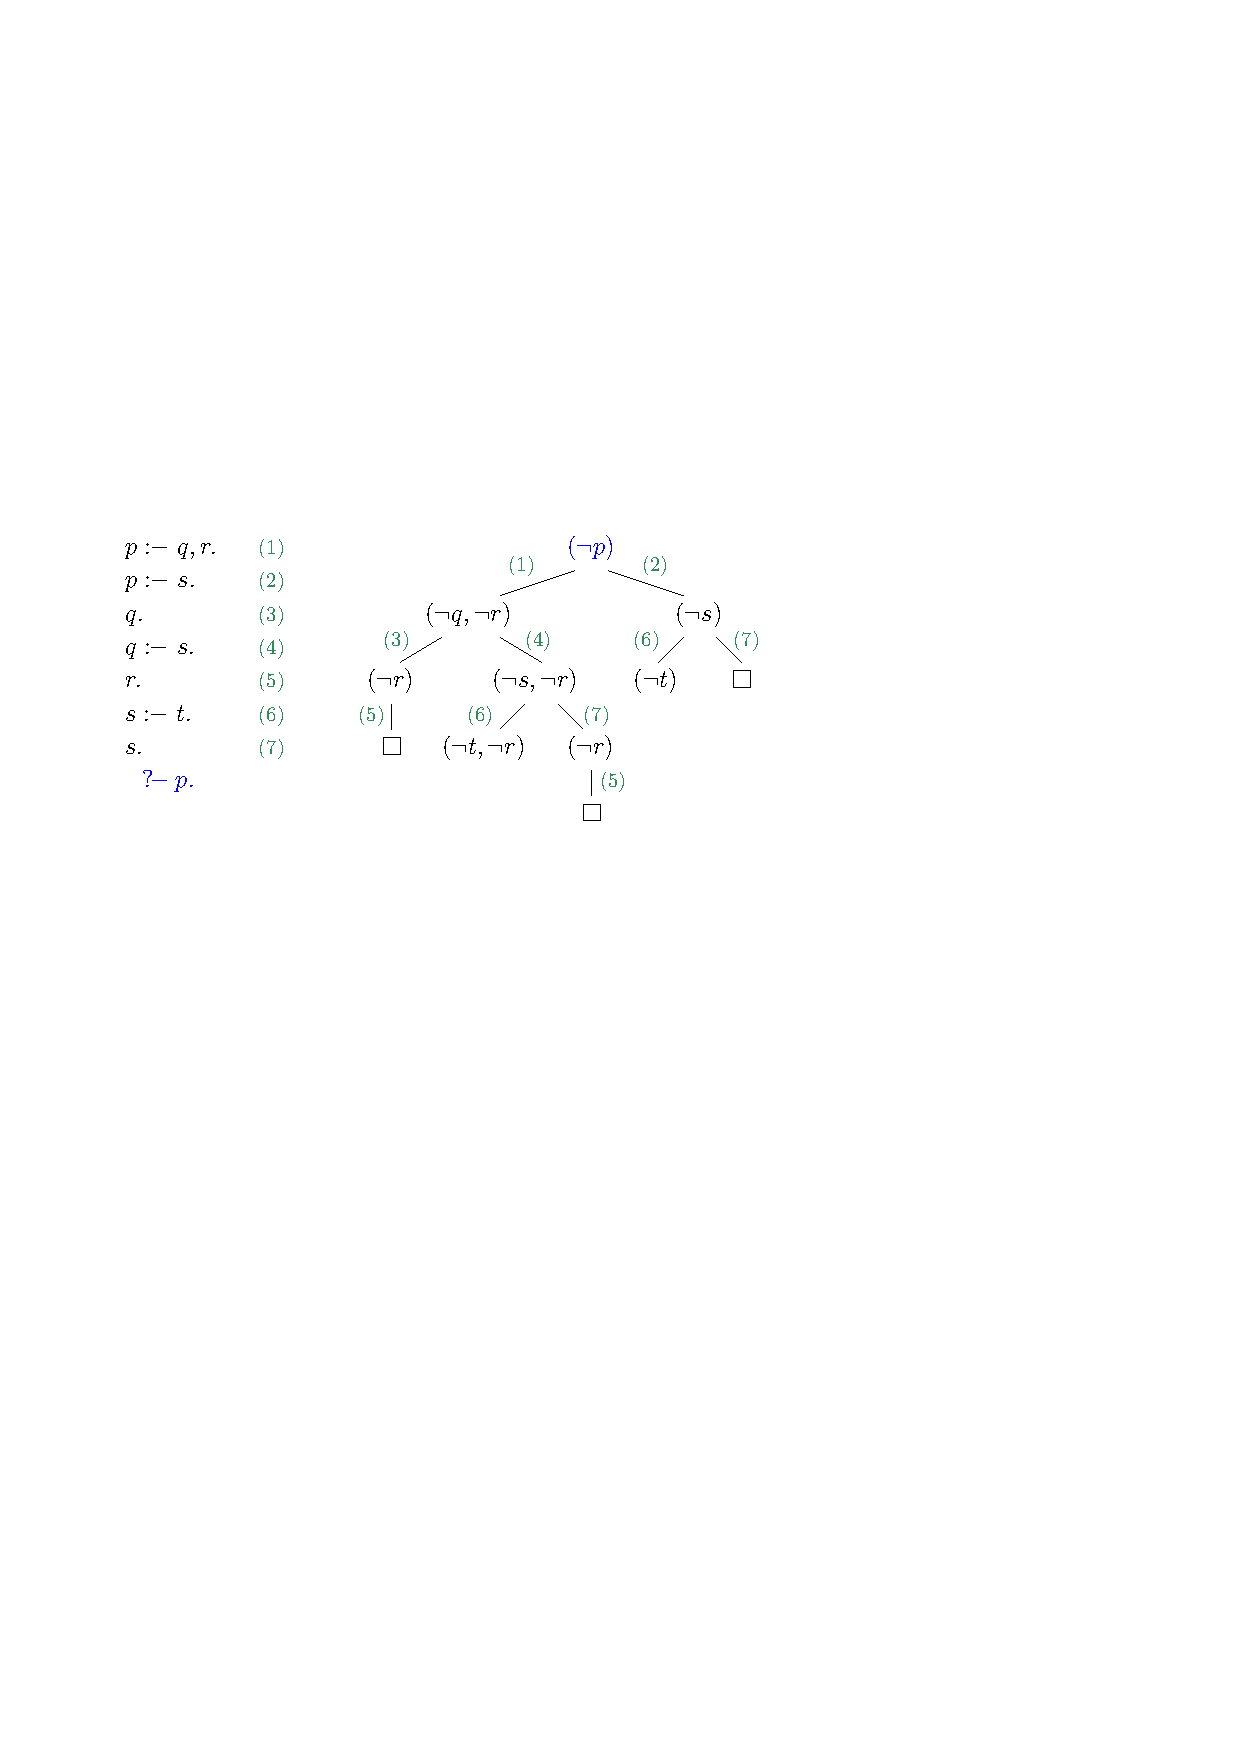
\includegraphics[scale=0.9]{files/rezoluceSLDstrom.pdf}}
% \smallskip

% %{\it Interpret Prologu prochází tímto SLD-stromem.}

% %%%%%%%%%%%%%%%%%%%%%%%%%%%%%%%%%%%%%%%%%%%%%%%%%%%%%%5

% \subsubsection*{Závěrečné poznámky}

% \begin{itemize}
% \item Interpret Prologu \myblue{prochází} SLD-strom, způsob není předepsán.

% \item Implementace, které používají \myblue{DFS}, nezachovávají úplnost.

% \smallskip
% \centerline{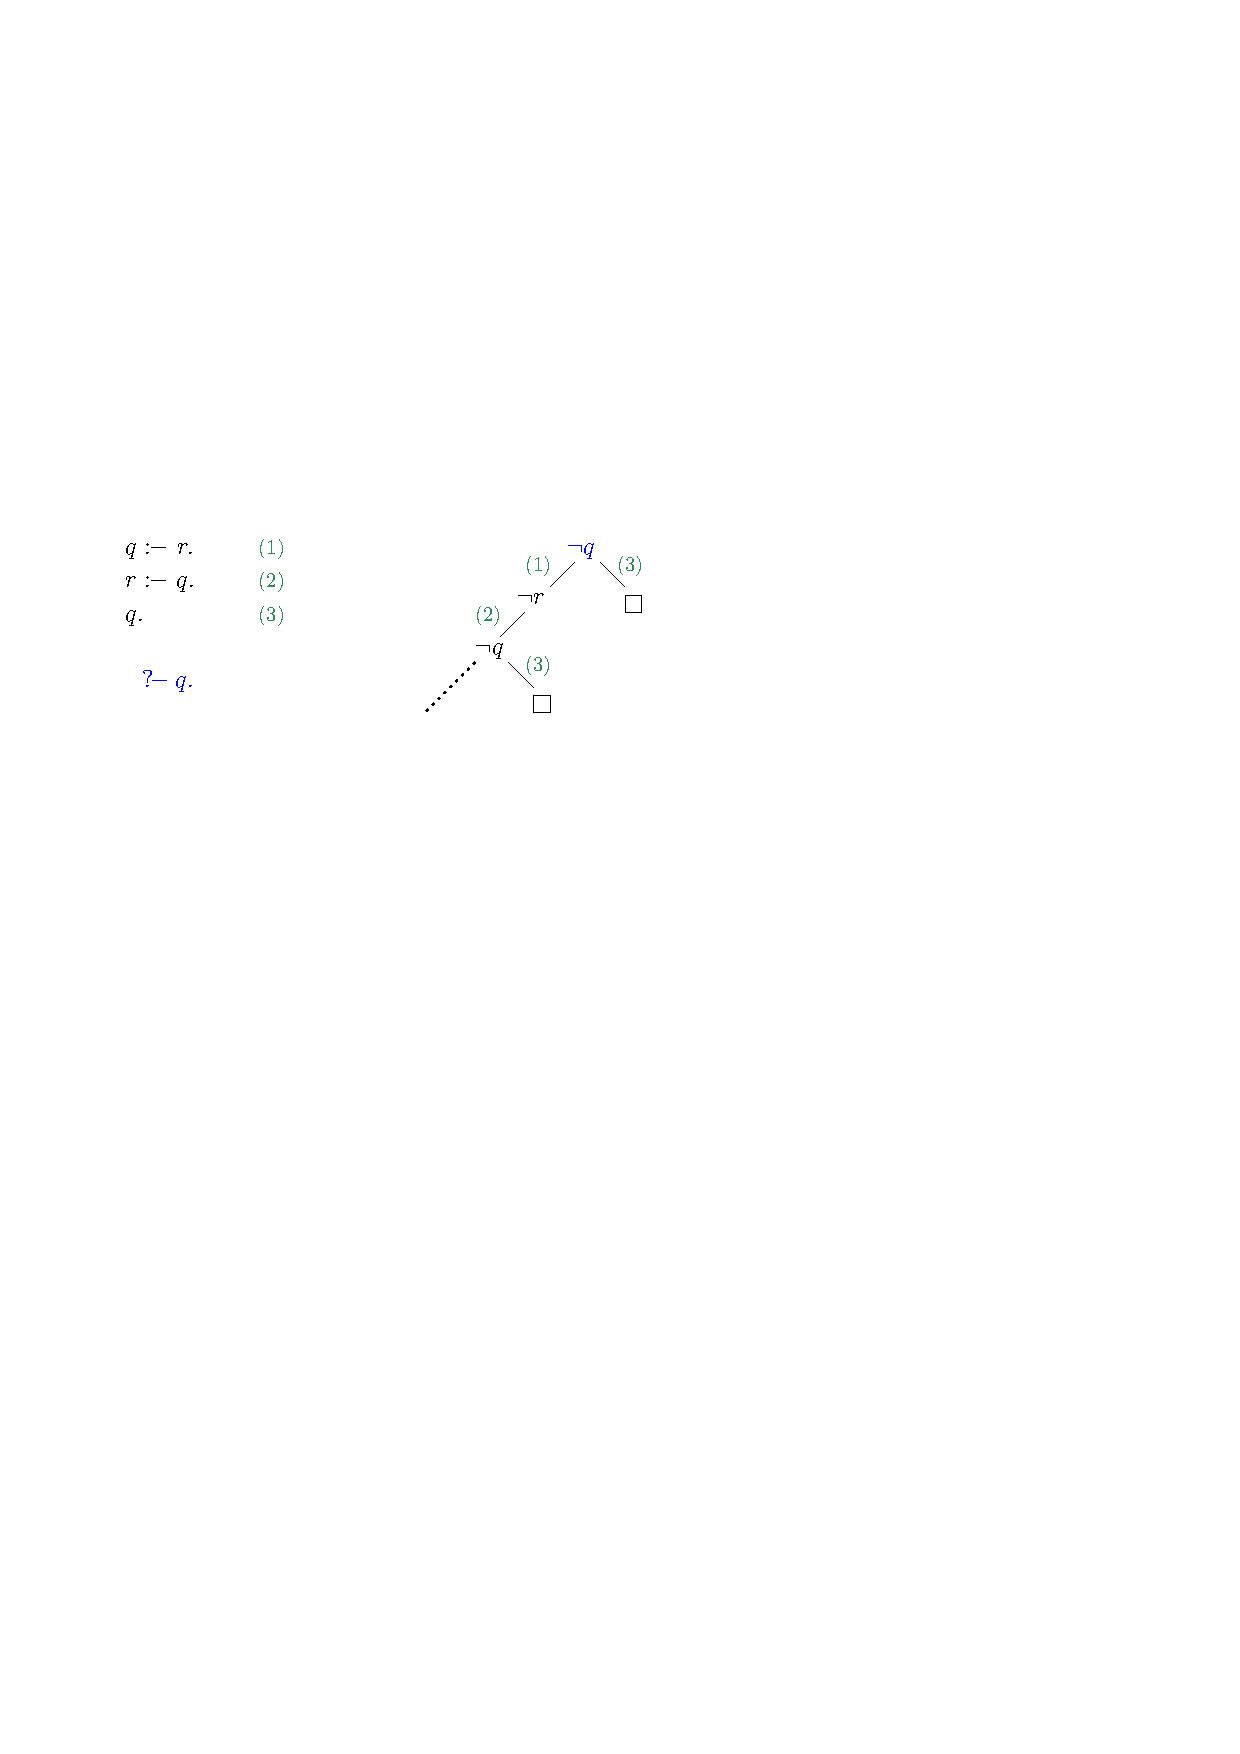
\includegraphics[scale=0.9]{files/rezoluceneuplnost.pdf}}
% \smallskip

% \item Jistou kontrolu nad prohledáváním poskytuje !, tzv. \myblue{řez}.

% \item Při povolení \myblue{negace} nastanou potíže se sémantikou programů.

% \item Síla rezoluční metody bude více patrná v predikátové logice.
% \end{itemize}

% % :from slides


% \part{Predikátová logika}

% \chapter{Syntaxe a sémantika predikátové logiky}

Kurzy logiky vesměs začínají výrokovou logikou, která je pro svou jednoduchost vhodnější k prvnímu seznámení. Plná síla logiky v informatice se ale projeví teprve s použitím logiky predikátové.
Začněme neformálním úvodem, ve kterém ilustrujeme základní aspekty predikátové logiky. K formálnímu výkladu se vrátíme v následujících sekcích.

\section{Úvod}
Připomeňme, že ve výrokové logice jsme popisovali svět pomocí \emph{výroků} složených z \emph{prvovýroků}---odpovědí na zjišťovací (ano/ne) otázky o světě. V predikátové logice (prvního řádu)\footnote{V logice druhého řádu máme také proměnné reprezentující množiny individuí nebo i množiny $n$-tic, tj. relace na množině individuí.} jsou základním stavebním kamenem \emph{proměnné} reprezentující \emph{individua}---nedělitelné objekty z nějaké množiny: např. přirozená čísla, vrcholy grafu, nebo stavy mikroprocesoru. 

Tato individua mohou mít určité vlastnosti a vzájemné vztahy, kterým říkáme \emph{predikáty}, např. `$\mathrm{Leaf}(x)$' nebo `$Edge(x,y)$' mluvíme-li o grafu, nebo `$x\leq y$' v přirozených číslech. Kromě toho mohou individua vstupovat do funkcí, např. `$\mathrm{lowest\_common\_ancestor}(x,y)$' v zakořeněném stromu, `$\mathrm{succ}(x)$' nebo `$x+y$' v přirozených číslech, a být \emph{konstantami} se speciálním významem, např. `$\mathrm{root}$' v zakořeněném stromu, `$0$' v přirozených číslech. 

\emph{Atomické formule} popisují predikát (včetně predikátu \emph{rovnosti} $=$) o proměnných nebo o \emph{termech} (`výrazech' složených\footnote{Podobně jako vytváříme aritmetické výrazy.} z funkcí popř. konstant). A složitější tvrzení (\emph{formule}) budujeme z atomických formulí pomocí logických spojek, a dvou \emph{kvantifikátorů}: 
\begin{itemize}
    \item $\forall x$ ``pro všechna individua (reprezentovaná proměnnou $x$),'' a
    \item $\exists x$ ``existuje individuum (reprezentované proměnnou $x$)''.
\end{itemize}
Uveďme příklad: tvrzení \textit{``Každý, kdo má dítě, je rodič.''} bychom mohli formalizovat následující formulí:
$$
(\forall x)((\exists y)\mathrm{child\_of}(y,x)\limplies\mathrm{is\_parent}(x))
$$
kde $\mathrm{child\_of}(y,x)$ je binární predikát vyjadřující, že individuum reprezentované proměnnou $y$ je dítětem individua reprezentovaného proměnnou $x$, a $\mathrm{is\_parent}(x)$ je unární predikát (tj. `vlastnost') vyjadřující, že individuum reprezentované $x$ je rodič.

Jak je to s platností této formule? To záleží na konkrétním \emph{modelu} světa/systému, který nás zajímá. Model je (neprázdná) množina objektů spolu s unární relací (tj. podmnožinou) \emph{interpretující} \emph{unární relační symbol} $\mathrm{is\_parent}$ a binární relací interpretující \emph{binární relační symbol} $\mathrm{child\_of}$. Tyto relace mohou být obecně jakékoliv a snadno sestrojíme model, kde formule neplatí.\footnote{Vezměme například jednoprvkovou množinu $A=\{a\}$, a relace $\mathrm{child\_of}^A=\{a\}$, $\mathrm{parent}^A=\emptyset$, tedy jediný objekt je svým vlastním dítětem, ale není rodičem.} Pokud ale modelujeme například všechny lidi na světě, a relace mají svůj přirozený význam, potom formule bude platit.\footnote{Při formalizaci musíme být velmi opatrní, abychom nepřidali dodatečné předpoklady, které v modelovaném systému nemusí platit. Zde se například schovává předpoklad, že má-li někdo dítě, musí to být jeho dítě.}

Podívejme se na ještě jeden příklad, tentokrát i s funkčními symboly a s konstantním symbolem: ``Je-li $x_1\leq y_1$ a $x_2\leq y_2$, potom platí $(y_1 \cdot y_2)-(x_1\cdot x_2)\geq 0$.'' Výsledná formule by mohla vypadat takto:
$$
\varphi=(x_1\leq y_1)\land (x_2\leq y_2)\limplies ((y_1 \cdot y_2)+(-(x_1\cdot x_2))\geq 0)
$$
Vidíme dva binární relační symboly ($\leq,\geq$), binární funkční symbol $+$, unární funkční symbol $-$, a konstantní symbol $0$. 

Modelem, ve kterém formule platí, je množina přirozených čísel $\mathbb N$ s binárními funkcemi $+^\mathbb N,\cdot^\mathbb N$, unární funkcí $-^\mathbb N$, a konstantou $0^\mathbb N=0$. Vezmeme-li ale podobně množinu celých čísel, formule už platit nebude.

\begin{remark}
Mohli bychom chápat symbol $-$ jako binární operaci, obvykle se ale zavádí jako unární. Pro konstantní symbol $0$ používáme (jak je zvykem) stejný symbol, jako pro přirozené číslo 0. Ale pozor, v našem modelu může být tento konstantní symbol interpretován jako jiné číslo, nebo náš model vůbec nemusí sestávat z čísel!
\end{remark}

Ve formuli nejsou žádné kvantifikátory (takovým formulím říkáme \emph{otevřené}), proměnné $x_1,x_2,y_1,y_2$ jsou \emph{volné proměnné} této formule (nejsou \emph{vázané} žádným kvantifikátorem), píšeme $\varphi(x_1,x_2,y_1,y_2)$. Sémantiku této formule chápeme stejně, jako formule
$$
(\forall x_1)(\forall x_2)(\forall y_1)(\forall y_2)\varphi(x_1,x_2,y_1,y_2)
$$

Výraz $(y_1 \cdot y_2)+(-(x_1\cdot x_2))$ je příkladem \emph{termu}, výrazy $(x_1\leq y_1)$, $(x_2\leq y_2)$ a $((y_1 \cdot y_2)+(-(x_1\cdot x_2))\geq 0)$ jsou \emph{atomické (pod)formule}. V čem spočívá rozdíl? Máme-li konkrétní model, a konkrétní \emph{ohodnocení proměnných} individui (prvky) tohoto modelu, potom atomickým formulím lze přiřadit pravdivostní hodnotu. Lze je tedy kombinovat s logickými spojkami do složitějších `logických výrazů', tj. formulí. Na druhou stranu `výsledkem' termu (při daném ohodnocení) je nějaké konkrétní individuum z modelu.

Upozorníme ještě na to, že v zápisu formule $\varphi$ jsme použili infixový zápis pro funkční symboly $+,\cdot$ a pro relace $\leq,\geq$, a podobné konvence o uzávorkování jako ve výrokové logice. Jinak bychom formuli $\varphi$ zapsali takto:
$$
((\leq (x_1,y_1) \land \leq(x_2,y_2))\limplies \leq(+(\cdot (y_1,y_2),-(\cdot(x_1,x_2))),0))
$$


\begin{exercise}
Najděte vhodnou definici pojmu \emph{stromu formule} (zobecňující \emph{strom výroku} z výrokové logiky) a nakreslete strom formule $(\forall x_1)(\forall x_2)(\forall y_1)(\forall y_2)\varphi(x_1,x_2,y_1,y_2)$.
\end{exercise}



Nyní začneme tím, že formalizujeme tento koncept ``\emph{modelu}'', tzv. \emph{strukturu}. Zbytek kapitoly sleduje osnovu výkladu o výrokové logice: představíme syntaxi, následně sémantiku, a nakonec pokročilejší vlastnosti formulí, teorií, a struktur. Na závěr si ukážeme jednu jednoduchou, ale velmi užitečnou aplikaci predikátové logiky, takzvanou \emph{definovatelnost} podmnožin a relací, která je základem \emph{relačních databází} (např. SQL), a ještě jednou se podíváme na vztah výrokové a predikátové logiky.

\section{Struktury}

Nejprve specifikujeme, jakého \emph{typu} bude daná struktura, tj. jaké bude mít relace, funkce (jakých arit) a konstanty, a jaké symboly pro ně budeme používat. Této formální specifikaci se někdy říká \emph{typ}, my budeme říkat \emph{signatura}.\footnote{Signaturu si můžete představovat analogicky definici \emph{třídy} v OOP, struktury potom odpovídají \emph{objektům} této třídy (v `programovacím jazyce' teorie množin).} Připomeňme, že \emph{konstanty} můžeme chápat jako funkce arity 0 (tj. funkce bez vstupů).

\begin{definition}
    \emph{Signatura} je dvojice $\langle\mathcal R,\mathcal F\rangle$, kde $\mathcal R,\mathcal F$ jsou disjunktní množiny symbolů (\emph{relační} a \emph{funkční}, ty zahrnují \emph{konstantní}) spolu s danými aritami (tj. danými funkcí $\mathrm{ar}\colon \mathcal R\cup\mathcal F\to\mathbb N$) a neobsahující symbol `$=$' (ten je rezervovaný pro \emph{rovnost}). 
    
\end{definition}

Často ale budeme signaturu zapisovat jen výčtem symbolů, bude-li jejich arita a to, zda jsou relační nebo funkční, zřejmé z kontextu. Uveďme několik příkladů signatur:
\begin{itemize}
    \item $\langle E \rangle$ signatura \emph{grafů}: $E$ je binární relační symbol (struktury jsou uspořádané grafy),
    \item $\langle \leq \rangle$ signatura \emph{částečných uspořádání}: stejná jako signatura grafů, jen jiný symbol,\footnote{Ne každá struktura v této signatuře je částečné uspořádání, k tomu ještě potřebujeme, aby splňovala příslušné \emph{axiomy}.}
    \item $\langle +, -, 0\rangle$ signatura \emph{grup}: $+$ je binární funkční, $-$ unární funkční, $0$ konstantní symbol
    \item $\langle +, -, 0,\cdot,1\rangle$ signatura \emph{těles}: $\cdot$ je binární funkční, $1$ konstantní symbol
    \item $\langle +, -, 0,\cdot,1,\leq\rangle$ signatura \emph{uspořádaných těles}: $\leq$ je binární relační symbol,
    \item $\langle -,\landsymb,\lorsymb,\bot,\top\rangle$ signatura \emph{Booleových algeber}: $\landsymb,\lorsymb$ jsou binární funkční symboly, $\bot,\top$ jsou konstantní symboly,
    \item $\langle S,+,\cdot,0,\leq\rangle$ signatura \emph{aritmetiky}: $S$ je unární funkční symbol (`successor').
\end{itemize}
Kromě běžných symbolů relací, funkcí a konstant (známých např. z logiky nebo z aritmetiky) typicky používáme pro relační symboly $P,Q,R,\dots$, pro funkční symboly $f,g,h,\dots$, a pro konstantní symboly $c,d,a,b,\dots$

\emph{Strukturu} dané signatury získáme tak, že na nějaké neprázdné \emph{doméně} zvolíme \emph{realizace} (také říkáme \emph{interpretace}) všech relačních a funkčních symbolů (a konstant), tj. konkrétní relace resp. funkce příslušných arit. (V případě konstantního symbolu je jeho realizací zvolený prvek z domény.)\footnote{Na tom, jaké konkrétní symboly v signatuře použijeme, nezáleží, můžeme je interpretovat libovolně. Například to, že máme symbol $+$ neznamená, že by jeho interpretace musela mít cokoliv společného se sčítáním (tedy kromě toho, že to bude také binární funkce).}

\begin{example} \label{example:signatures}
    Formální definice \emph{struktury} je uvedena níže, nejprve si ukážeme několik příkladů:
\begin{itemize}
    \item Struktura v prázdné signatuře $\langle\ \rangle$ je libovolná neprázdná množina.\footnote{Jak uvidíme v definici níže, formálně vzato je to trojice $\langle A,\emptyset,\emptyset\rangle$, ale tento rozdíl budeme zanedbávat.} (Nemusí být konečná, dokonce ani spočetná!)
    \item Struktura v signatuře grafů je $\mathcal G=\langle V,E\rangle$, kde $V\neq\emptyset$ a $E\subseteq V^2$, říkáme jí \emph{orientovaný graf}. 
    \begin{itemize}
        \item Je-li $E$ irreflexivní a symetrická, jde o \emph{jednoduchý} graf (tj. neorientovaný, bez smyček).
        \item Je-li $E$ reflexivní, tranzitivní, a antisymetrická, jde o \emph{částečné uspořádání}.
        \item Je-li $E$ reflexivní, tranzitivní, a symetrická, mluvíme o \emph{ekvivalenci}.
    \end{itemize}
    \item Struktury v signatuře částečných uspořádání jsou tytéž, jako v signatuře grafů, signatury se liší jen použitým symbolem. (Tedy ne každá struktura v signatuře částečných uspořádání je částečné uspořádání!)
    \item Struktury v signatuře grup jsou například následující \emph{grupy}:
    \begin{itemize}
        \item $\underline{\mathbb Z_n}=\langle\mathbb Z_n,+,-,0\rangle$, \emph{aditivní grupa celých čísel modulo $n$} (operace jsou modulo $n$).\footnote{Zde $\underline{\mathbb Z_n}$ znamená strukturu, zatímco $\mathbb Z_n=\{0,1,\dots,n-1\}$ jen její doménu. Často se ale toto nerozlišuje a symbol $\mathbb Z_n$ se používá jak pro celou strukturu, tak jen její doménu. Podobně $+,-,0$ jsou jak symboly, tak i jejich interpretace. To je běžně používané značení, je klíčové být si vždy vědomi toho, v jakém významu daný symbol na daném místě používáme.}
        \item $\mathcal S_n=\langle \mathrm{Sym}_n,\circ,{}^{-1},\mathrm{id}\rangle$ je \emph{symetrická grupa} (grupa všech permutací) na $n$ prvcích.
        \item $\underline{\mathbb Q}^*=\langle \mathbb Q\setminus\{0\},\cdot,{}^{-1},1\rangle$ je \emph{multiplikativní grupa (nenulových) racionálních čísel}. Všimněte si, že interpretací \emph{symbolu} $0$ je \emph{číslo} $1$.
    \end{itemize}
    Všechny tyto struktury \emph{splňují axiomy teorie grup}, snadno ale najdeme jiné struktury, které tyto axiomy nesplňují, a nejsou tedy grupami. Například změníme-li ve struktuře $\mathbb Z_n$ interpretaci symbolu $+$ na funkci $\cdot$ (modulo $n$).
    \item Struktury $\underline{\mathbb Q}=\langle \mathbb Q, +, -, 0,\cdot,1,\leq\rangle$ a $\underline{\mathbb Z}=\langle \mathbb Z, +, -, 0,\cdot,1,\leq\rangle$, se standardními operacemi a uspořádáním, jsou v signatuře uspořádaných těles (ale jen první z nich je uspořádaným tělesem).
    \item $\underline{\mathcal P(X)}=\langle \mathcal P(X),\bar{},\cap,\cup,\emptyset,X\rangle$, tzv. \emph{potenční algebra} nad množinou $X$, je to struktura v signatuře Booleových algeber. (\emph{Booleova algebra} je to pokud $X\neq\emptyset$
    \item $\underline{\mathbb N}=\langle \mathbb N,S,+,\cdot,0,\leq\rangle$, kde $S(x)=x+1$, a ostatní symboly jsou interpretovány standardně, je \emph{standardní model aritmetiky}.
\end{itemize}
\end{example}



\begin{definition}[Struktura]
\emph{Struktura v signatuře} $\langle\mathcal R,\mathcal F\rangle$ je trojice $\A=\langle A, \mathcal R^\A,\mathcal F^\A \rangle$, kde
\begin{itemize}
   \item  $A$ je neprázdná množina, říkáme jí \emph{doména} (také \emph{univerzum}),
   \item $\mathcal R^\A=\{R^\A\mid R\in\mathcal R\}$ kde $R^\A\subseteq A^{\mathrm{ar}(R)}$ je \emph{interpretace} relačního symbolu $R$,
   \item $\mathcal F^\A=\{f^\A\mid f\in\mathcal F\}$ kde $f^\A\colon A^{\mathrm{ar}(R)}\to A$ je \emph{interpretace} funkčního symbolu $f$ (speciálně pro konstantní symbol $c\in\mathcal F$ máme $c^\A\in A$).
\end{itemize}


\end{definition}


\begin{exercise}
Uvažme signaturu \emph{$n$ konstant} $\langle c_1,c_2,\dots,c_n\rangle$. Jak vypadají struktury v této signatuře? Popište např. všechny nejvýše pětiprvkové struktury v signatuře tří konstant. (Interpretace konstant nemusí být různé!)
A jak je tomu v případě signatury \emph{spočetně mnoha konstant} $\langle c_1,c_2,\dots\rangle=\langle c_i\mid i\in\mathbb N\rangle$?
\end{exercise}


\section{Syntaxe}

V této sekci představíme syntaxi predikátové logiky (prvního řádu). Srovnejte co má syntaxe společného, a jak se liší, od syntaxe výrokové logiky.


\subsection{Jazyk}

Při specifikaci jazyka nejprve stanovíme, v jakého typu jsou struktury, které chceme popisovat, tj. určíme \emph{signaturu}. Dále přidáme informaci, zda je jazyk \emph{s rovností} nebo ne, tj. zda ve formulích můžeme také používat symbol `$=$' vyjadřující rovnost (identitu) prvků v doméně struktur.\footnote{Ve většině aplikací budeme používat jazyky s rovností. V některých speciálních oblastech se ale hodí rovnost nemít. Například pokud se zabýváme velmi rychlými výpočetními modely: zjistit, které proměnné se sobě rovnají, vyžaduje najít tranzitivní uzávěr rovností daných formulí, což je relativně výpočetně náročný problém.} Do jazyka patří následující:
\begin{itemize}
    \item spočetně mnoho \emph{proměnných} $x_0,x_1,x_2,\dots$ (ale píšeme také $x,y,z,\dots$; množinu všech proměnných označíme $\Var$),
    \item \emph{relační}, \emph{funkční} a \emph{konstantní symboly} ze signatury, a symbol $=$ jde-li o jazyk s rovností,
    \item \emph{univerzální} a \emph{existenční} \emph{kvantifikátory} $(\forall x),(\exists x)$ pro každou proměnnou $x\in\Var$,\footnote{Kvantifikátor chápeme jako jediný symbol, tedy $(\forall x)$ \emph{neobsahuje} proměnnou $x$. Někdy se také používají symboly $\forall_x,\exists_x$.}
    \item symboly pro logické spojky \( \neg,\landsymb,\lorsymb, \limpliessymb, \liffsymb \) a závorky \( (,) \).
\end{itemize}
Podobně jako symbol $\lbinsymb$ zastupující libovolnou binární logickou spojku budeme někdy psát $(Qx)$ pro kvantifikátor $(\forall x)$ nebo $(\exists x)$.

Symbolům ze signatury říkáme \emph{mimologické}, ostatní jsou \emph{logické}. Jazyk musí obsahovat alespoň jeden relační symbol (buď rovnost, nebo v signatuře).\footnote{Jinak bychom v jazyce nemohli vybudovat žádná `tvrzení' (\emph{formule}), viz níže.}

Jazyk tedy specifikujeme pomocí signatury a informace `s rovností' (popř. `bez rovnosti'). Například:
\begin{itemize}
    \item Jazyk $L=\langle\rangle$ s rovností je jazyk \emph{čisté rovnosti},
    \item jazyk $L=\langle c_0,c_1,c_2,\dots\rangle$ s rovností je jazyk \emph{spočetně mnoha konstant},
    \item jazyk \emph{uspořádání} je $\langle \leq \rangle$ s rovností,
    \item jazyk \emph{teorie grafů} je $\langle E \rangle$ s rovností,
    \item jazyky \emph{teorie grup, teorie těles, teorie uspořádaných těles, Booleových algeber, aritmetiky} jsou jazyky s rovností odpovídající signaturám z Příkladu \ref{example:signatures}
\end{itemize}


\subsection{Termy}

Termy jsou syntaktické `výrazy' složené z proměnných, konstantních symbolů a funkčních symbolů.

\begin{definition}[Termy]
    \emph{Termy} jazyka $L$ jsou konečné nápisy definované induktivně:
    \begin{itemize}
        \item každá proměnná a každý konstantní symbol z $L$ je term,
        \item je-li $f$ funkční symbol z $L$ arity $n$ a jsou-li $t_1,\dots,t_n$ termy, potom nápis $f(t_1,t_2,\dots,t_n)$ je také term.
    \end{itemize}
    Množinu všech \emph{termů} jazyka $L$ označíme $\Term_L$. 
\end{definition}

Při zápisu termů obsahujících binární funkční symbol můžeme používat \emph{infixový} zápis, např. $(t_1+t_2)$ znamená $+(t_1,t_2)$. Závorky někdy vynecháváme, je-li struktura termu (`priorita operátorů') zřejmá.

\emph{Podterm} je podřetězec termu, který je sám termem (je to tedy buď celý term, nebo se vyskytl jako nějaké $t_i$ při konstrukci termu).

Pokud term neobsahuje proměnnou, říkáme mu \emph{konstantní (ground)}, například $((S(0)+S(0))\cdot S(S(0)))$ je konstantní term v jazyce aritmetiky.\footnote{Pozor, termy jsou čistě syntaktické, můžeme používat jen symboly z jazyka, nikoliv prvky struktury, tedy např. $(1+1)\cdot 2$ \emph{není} term v jazyce aritmetiky! (Mohli bychom ale \emph{definovat} nové konstantní symboly $1,2$ jako zkratky za $S(0)$ a $S(S(0))$ a \emph{rozšířit} tak náš jazyk, viz Sekce \ref{subsection:extension-by-definition}.)}

\emph{Strom termu $t$}, označme $\Tree(t)$, je definován podobně jako strom výroku, v listech jsou proměnné nebo konstantní symboly, ve vnitřních vrcholech jsou funkční symboly, jejichž arita je rovna počtu synů.

\begin{example}\label{example:terms}
    Nakresleme stormy termů (a) $(S(0) + x) \cdot y$ v jazyce aritmetiky, (b) $\neg (x\land y)\lor \bot$ v jazyce Booleových algeber. Zde $\neg,\land,\lor$ nejsou logické spojky z jazyka, ale mimologické symboly ze signatury Booleových algeber (byť používáme stejné symboly)! Termy v tomto jazyce můžeme chápat jako výrokové formule (s konstantami pro spor a tautologii), viz Sekce~\ref{section:relationship-propositional-predicate-logic}.   
    Na obrázku~\ref{figure:terms} jsou nakresleny stromy těchto termů.
    
    \begin{figure}\label{figure:terms}
    \tikzset{every label/.style = {text=red}}
    \begin{minipage}{.49\textwidth}
        \centering
        \begin{forest}
            for tree={math content,circle,draw=blue!20,fill=blue!10,minimum size=24pt}
            [\cdot 
                [+ 
                    [S
                        [0]                    
                    ] 
                    [x]
                ]
                [y]
            ]
        \end{forest}

        (a) $(S(0) + x) \cdot y$ v jazyce aritmetiky
    \end{minipage}
    \begin{minipage}{.49\textwidth}
        \centering
        \begin{forest}
            for tree={math content,circle,draw=blue!20,fill=blue!10,minimum size=24pt}
            [\lor 
                [\neg 
                    [\land
                        [x]
                        [y]                    
                    ]
                ]
                [\bot]
            ]
        \end{forest}
        
        (b) $\neg (x\land y)\lor \bot$ v jazyce Booleových algeber
    \end{minipage}
    \caption{Strom termu}
    \end{figure}
\end{example}

Není těžké uhádnout, jaká bude \emph{sémantika} termů. Máme-li  konkrétní strukturu, odpovídá term funkci na její doméně: vstupem je ohodnocení proměnných prvky domény, konstantní a funkční symboly jsou nahrazeny jejich interpretacemi, a výstupem je hodnota (prvek domény) v kořeni. Formálněji ale až v Sekci \ref{section:predicate-semantics}.


\subsection{Formule}

Termům nelze v žádném smyslu přiřadit pravdivostní hodnotu, k tomu potřebujeme \emph{predikát} (relační symbol nebo rovnost), který mluví o `vztahu' termů: v konkrétní struktuře při konkrétním ohodnocení proměnných prvky z domény je tento vztah buď splněn, nebo nesplněn. 

Nejjednoduššími \emph{formulemi} jsou \emph{atomické formule}. Z nich potom vybudujeme pomocí logických spojek a kvantifikátorů všechny formule.


\begin{definition}[Atomická formule]
    \emph{Atomická formule} jazyka $L$ je nápis $R(t_1,\dots,t_m)$, kde $R$ je $n$-ární relační symbol z $L$ (včetně $=$ jde-li o jazyk s rovností) a $t_i\in\Term_L$. %Množinu všech \emph{atomických formulí} jazyka $L$ označíme $\AFm_L$. 
\end{definition}

U binárních relačních symbolů často používáme infixový zápis, např. atomickou formuli $\leq(x,y)$ zapíšeme jako $x\leq y$, a (je-li jazyk s rovností) místo $=(t_1,t_2)$ budeme psát $t_1=t_2$.

\begin{example}
    Uveďme několik příkladů atomických formulí:
    \begin{itemize}
        \item $R(f(f(x)),c, f(d))$ kde $R$ je ternární relační, $f$ unární funkční, $c,d$ konstantní symboly,
        \item $(x\cdot x)+(y\cdot y)\leq (x+y)\cdot(x+y)$ v jazyce uspořádaných těles,
        \item $x\cdot y\leq (S(0)+x)\cdot y$ v jazyce aritmetiky,
        \item $\neg(x\land y)\lor\bot=\bot$ v jazyce Booleových algeber        
    \end{itemize}
\end{example}


\begin{definition}[Formule]
    \emph{Formule} jazyka $L$ jsou konečné nápisy definované induktivně: 
    \begin{itemize}
        \item každá atomická formule jazyka $L$ je formule,
        \item jsou-li $\varphi,\psi$ formule, potom $(\varphi\land\psi)$, $(\varphi\lor\psi)$, $(\varphi\limplies\psi)$, a $(\varphi\liff\psi)$ jsou také formule,
        \item je-li $\varphi$ formule a $x$ proměnná, potom $((\forall x)\varphi)$ a $((\exists x)\varphi)$ jsou také formule.
        \end{itemize}    
    %Množinu všech \emph{formulí} jazyka $L$ označíme $\Fm_L$.
\end{definition}
\emph{Podformule} je podřetězec, který je sám o sobě formulí. \emph{Strom formule}, označíme $\Tree(\varphi)$, je definován takto: strom atomické formule $\varphi=R(t_1,\dots,t_n)$ má v kořeni relační symbol $R$, a k němu jsou připojeny stromy $\Tree(t_i)$. Není-li $\varphi$ atomická, strom zkonstruujeme obdobně jako strom výroku.\footnote{Kvantifikátory mají, podobně jako negace, jediného syna.} Při zápisu formulí používáme obdobné konvence jako ve výrokové logice, přičemž kvantifikátory mají stejnou prioritu jako $\neg$ (vyšší než ostatní logické spojky). Místo $((\forall x)\varphi$) tedy můžeme psát $(\forall x)\varphi$.\footnote{Někdy se také nepíší závorky v kvantifikátorech, tj. jen $\forall x\varphi$, my je ale pro přehlednost psát budeme.}

\begin{example}\label{example:formula} Příkladem formule v jazyce aritmetiky je $(\forall x)(x\cdot y\leq (S(0)+x)\cdot y)$. Její strom je znázorněn na Obrázku \ref{figure:tree-of-formula}.
    \begin{figure}
        \centering
        \begin{forest}
            for tree={math content,circle,draw=blue!20,fill=blue!10,minimum size=22pt}
            [\forall x
                [\leq 
                    [\cdot [x] [y]] 
                    [\cdot [+ [S [0]] [x]] [y]]
                ]
            ]
        \end{forest}
            \caption{Strom formule $(\forall x)(x\cdot y\leq (S(0)+x)\cdot y)$}\label{figure:tree-of-formula}
        \end{figure}
\end{example}


\subsubsection{Volné a vázané proměnné}

Význam formule\footnote{Přesněji, její \emph{pravdivostní hodnota}, kterou formálně definujeme níže v Sekci \ref{subsection:truth-value-of-formula}.} může, nebo nemusí záviset na proměnných, které se v ní vyskytují: srovnejte $x\leq 0$ a $(\exists x)(x\leq 0)$ (a co teprve $x\leq 0 \lor (\exists x)(x\leq 0)$). Nyní tento koncept upřesníme a zavedeme potřebnou terminologii.


\emph{Výskytem} proměnné $x$ ve formuli $\varphi$ myslíme list $\Tree(\varphi)$ označený $x$. \footnote{Proměnná $x$ se tedy \emph{nevyskytuje} v symbolu pro kvantifikátor $(Qx)$.} Výskyt je \emph{vázaný}, je-li součástí nějaké podformule (podstromu) začínající $(Qx)$. Není-li výskyt vázaný, je \emph{volný}. Proměnná je \emph{volná} ve $\varphi$, pokud má ve $\varphi$ volný výskyt, a \emph{vázaná} ve $\varphi$, pokud má ve $\varphi$ vázaný výskyt. Zápis $\varphi(x_1,\dots,x_n)$ znamená, že $x_1,\dots,x_n$ jsou všechny volné proměnné ve formuli $\varphi$.

\begin{example}
    Proměnná může být volná i vázaná, např. ve formuli $\varphi=(\forall x)(\exists y)(x\leq y)\lor x\leq z$ je první výskyt $x$ vázaný a druhý výskyt volný. (Nakreslete si strom formule!) Proměnná $y$ je vázaná (její jediný výskyt je vázaný) a $z$ je volná. Můžeme tedy psát $\varphi(x,z)$.
\end{example}

\begin{remark}
    Jak uvidíme níže, význam (\emph{pravdivostní hodnota}) formule závisí pouze na ohodnocení volných proměnných. Proměnné v kvantifikátorech, spolu s příslušnými vázanými výskyty, můžeme libovolně přejmenovat.   
\end{remark}

\subsubsection{Otevřené a uzavřené formule}

Často budeme mluvit o následujících dvou důležitých druzích formulí:

\begin{definition}[Otevřená a uzavřená formule]
Formule je \emph{otevřená}, neobsahuje-li žádný kvantifikátor, a \emph{uzavřená} (neboli \emph{sentence}), pokud nemá žádnou volnou proměnnou  
\end{definition}

\begin{example} Uveďme několik příkladů:
    \begin{itemize}
        \item formule $x+y\leq 0$ je otevřená,
        \item formule $(\forall x)(\forall y)(x+y\leq 0)$ je uzavřená (tedy je to sentence),
        \item formule $(\forall x)(x+y\leq 0)$ není ani otevřená, ani uzavřená,
        \item formule $(0+1=1)\land (1+1=0)$ je otevřená i uzavřená. 
    \end{itemize}
\end{example}

Každá atomická formule je otevřená, otevřené formule jsou jen kombinace atomických pomocí logických spojek. Formule může být otevřená i uzavřená zároveň, v tom případě jsou všechny její termy konstantní. Formule je uzavřená, právě když nemá žádnou volnou proměnnou.\footnote{Neplatí ale, že formule je otevřená, pokud nemá žádnou vázanou proměnnou, viz formule $(\forall x)0=1$.}

\begin{remark}
Jak uvidíme později, \emph{pravdivostní hodnota} formule závisí jen na ohodnocení jejích volných proměnných. Speciálně, sentence má v dané struktuře pravdivostní hodnotu 0 nebo 1 (nezávisle na ohodnocení proměnných). To je důvod, proč hrají sentence v logice důležitou roli.
\end{remark}

\subsection{Instance a varianty}

Jak jsme viděli, jedna proměnná se může ve formuli vyskytovat v různých `rolích'. Jde o velmi podobný princip jako v programování, kde jeden identifikátor může v programu znamenat různé proměnné (buď lokální, nebo globální). Pod pojmem \emph{instance} si představte `dosazení' (termu) do (globální) proměnné (nebo lépe `nahrazení' proměnné nějakým výrazem, který ji počítá), a pod pojmem \emph{varianta} `přejmenování' (lokální) proměnné. Vezměme například formuli $\varphi(x)$:
$$
P(x)\land (\forall x)(Q(x) \land (\exists x)R(x))
$$
První výskyt proměnné $x$ je volný, druhý je vázaný kvantifikátorem $(\forall x)$, a třetí je vázaný  $(\exists x)$. Pokud `dosadíme' za proměnnou $x$ term $t=1+1$, dostáváme \emph{instanci} formule $\varphi$, kterou označíme $\varphi(x/t)$:
$$
P(1+1)\land (\forall x)(Q(x) \land (\exists x)R(x))
$$
Můžeme také přejmenovat kvantifikátory ve formuli, tak získáme \emph{variantu} formule $\varphi$, např.:
$$
P(x)\land (\forall y)(Q(y) \land (\exists z)R(z))
$$
Jak víme, kdy a jak toto můžeme provést, abychom zachovali význam, tj. aby instance byla \emph{důsledkem} $\varphi$, a varianta byla s $\varphi$ \emph{ekvivalentní}? To nyní chceme zformalizovat.

\subsubsection{Instance}

Pokud do formule $\varphi$ \emph{dosadíme} za volnou proměnnou $x$ term $t$, požadujeme, aby výsledná formule `říkala' o $t$ `totéž', co $\varphi$ o $x$. 

\begin{example}
    Například formule $\varphi(x)=(\exists y)(x+y=1)$ říká o $x$, že `existuje $x-1$'. Term $t=1$ lze dosadit, neboť $\varphi(x/t)=(\exists y)(1+y=1)$ říká `existuje 1-1'. Ale term $t=y$ dosadit nelze, $(\exists y)(y+y=1)$ říká `1 je dělitelné 2'. Problém spočívá v tom, že term $t=y$ obsahuje proměnnou $y$, jež bude nově vázaná kvantifikátorem $(\exists y)$. Takové situaci se musíme vyhnout.
\end{example}

\begin{definition}[Substituovatelnost a instance]
    Term $t$ je \emph{substituovatelný} za proměnnou $x$ ve formuli $\varphi$, pokud po simultánním nahrazení všech volných výskytů $x$ ve $\varphi$ za $t$ nevznikne ve $\varphi$ žádný vázaný výskyt proměnné z $t$. V tom případě říkáme vzniklé formuli \emph{instance} $\varphi$ vzniklá substitucí $t$ za $x$, a označujeme ji $\varphi(x/t)$.
\end{definition}

\begin{remark}
    Všimněte si, že term $t$ \emph{není} substituovatelný za $x$ do $\varphi$, právě když $x$ má volný výskyt v nějaké podformuli $\varphi$ tvaru $(Qy)\psi$ a proměnná $y$ se vyskytuje v $t$. Speciálně, konstantní termy jsou vždy substituovatelné.    
\end{remark}

\subsubsection{Varianty}

Potřebujeme-li substituovat term $t$ do formule $\varphi$, můžeme to udělat vždy, pokud nejprve přejmenujeme všechny kvantifikované proměnné na zcela nové (tj. takové, které se nevyskytují ani ve $\varphi$ ani v $t$), a potom substituujeme $t$ do takto vzniklé \emph{varianty} formule $\varphi$.

\begin{definition}[Varianta]
   Má-li formule $\varphi$ podformuli tvaru $(Qx)\psi$ a je-li $y$ proměnná, taková, že
   \begin{itemize}
    \item $y$ je substituovatelná za $x$ do $\psi$ a
    \item $y$ nemá volný výskyt v $\psi$,
   \end{itemize} 
potom nahrazením podformule $(Qx)\psi$ formulí $(Qy)\psi(x/y)$ vznikne \emph{varianta} formule $\varphi$ v podformuli $(Qx)\psi$. \emph{Varianta} říkáme i výsledku postupné variace ve více podformulích.
\end{definition}

Všimněte si, že požadavek na proměnnou $y$ z definice varianty je vždy splněn, pokud se $y$ nevyskytuje ve formuli $\varphi$.

\begin{example}
    Mějme formuli $\varphi=(\exists x)(\forall y)(x\leq y)$. Potom:
\begin{itemize}
    \item $(\exists u)(\forall v)(u\leq v)$ je varianta $\varphi$,
    \item $(\exists u)(\forall u)(u\leq u)$ není varianta $\varphi$, neboť $y$ není substituovatelná za $x$ do $\varphi$,
    \item $(\exists x)(\forall x)(x\leq x)$ není varianta $\varphi$, neboť $x$ má volný výskyt $\psi=(x\leq y)$.
\end{itemize}   
\end{example}

Tím jsme uzavřeli výklad o syntaxi, následuje sémantika.


\section{Sémantika}\label{section:predicate-semantics}

Než se pustíme do formálnějšího výkladu, shrňme stručně sémantiku, tak jak jsme ji už naznačili v předchozích sekcích: 

\begin{itemize}
    \item modely jsou struktury dané signatury,
    \item formule platí ve struktuře, pokud platí při každém ohodnocení volných proměnných prvky z domény,
    \item hodnoty termů se vyhodnocují podle jejich stromů, kde symboly nahradíme jejich interpretacemi (relacemi, funkcemi, a konstantami z domény),
    \item z hodnot termů získáme pravdivostní hodnoty atomických formulí: je výsledná $n$-tice v relaci?
    \item hodnoty složených formulí vyhodnocujeme také podle jejich stromu, přičemž $(\forall x)$ hraje roli `konjunkce přes všechny prvky' a  $(\exists y)$ hraje roli `disjunkce přes všechny prvky' z domény struktury
\end{itemize}

Nyní formálněji:

\subsection{Modely jazyka}

\begin{definition}[Model jazyka]
\emph{Model jazyka $L$}, nebo také $L$-struktura, je libovolná struktura v signatuře jazyka $L$. \emph{Třídu} všech modelů jazyka označíme $\M_L$.
\end{definition}

\begin{remark}
V definici nehraje roli, zda je jazyk s rovností nebo bez. A proč nemůžeme mluvit o \emph{množině} všech modelů $\M_L$, proč musíme říkat \emph{třída}? Protože doménou struktury může být libovolná neprázdná množina, a `množina všech množin' neexistuje, je to klasický příklad tzv. vlastní třídy. Třída je \emph{`soubor'} všech množin splňujících danou vlastnost (popsatelnou v \emph{jazyce teorie množin}).
\end{remark}


\begin{example}
    Mezi modely jazyka uspořádání $L=\langle \leq \rangle$ patří následující struktury: $\langle \mathbb N,\leq\rangle$, $\langle \mathbb Q, > \rangle$, libovolný orientovaný graf $G=\langle V,E\rangle$, $\langle \mathcal P(X),\subseteq\rangle$. Ale také např. $\langle \mathbb C,R^\mathbb C\rangle$ kde $(z_1,z_2)\in R^\mathbb C$ právě když $|z_1|=|z_2|$ nebo $\langle \{0,1\},\emptyset\rangle$, což \emph{nejsou} částečná uspořádání.
\end{example}


\subsection{Hodnota termu}

Mějme term $t$ jazyka $L=\langle \mathcal R,\mathcal F\rangle$ (s rovností nebo bez), a $L$-strukturu $\A=\langle A,\mathcal R^\A,F^\A\rangle$. \emph{Ohodnocení proměnných} v množině $A$ je libovolná funkce $e:\Var\to A$.

\begin{definition}[Hodnota termu]
    \emph{Hodnota termu $t$ ve struktuře $\A$ při ohodnocení $e$}, kterou značíme $t^\A[e]$, je dána induktivně:
    \begin{itemize}
        \item $x^\A[e]=e(x)$ pro proměnnou $x\in\Var$,
        \item $c^\A[e]=c^\A$ pro konstantní symbol $c\in\mathcal F$, a
        \item je-li $t=f(t_1,\dots,t_n)$ složený term, kde $f\in\mathcal F$, potom:
        $$
        t^\A[e]=f^\A(t_1^\A[e],\dots,t_n^\A[e])
        $$
    \end{itemize}
\end{definition}

\begin{remark}
    Všimněte si, že hodnota termu závisí pouze na ohodnocení proměnných vyskytujících se v něm. Speciálně, je-li $t$ konstantní term, jeho hodnota na ohodnocení nezávisí.
    Obecně, každý term $t$ reprezentuje \emph{termovou funkci} $f_t^\A\colon A^k\to A$, kde $k$ je počet proměnných v $t$, a konstantním termům odpovídají konstantní funkce.
\end{remark}

\begin{example}
    Uveďme dva příklady:
    \begin{itemize}
        \item Hodnota termu $-(x\lor \bot)\land y$ v Booleově algebře $\underline{\mathcal P(\{0,1,2\})}$ při ohodnocení $e$ ve kterém $e(x)=\{1,2\}$ a $e(y)=\{2,3\}$ je $\{3\}$.
        \item Hodnota termu $x+1$ ve struktuře $\mathcal N=\langle\mathbb N,\cdot,3\rangle$ jazyka $L=\langle +,1\rangle$ při ohodnocení $e$ ve kterém $e(x)=2$ je $(x+1)^\mathcal N[e]=6$.
    \end{itemize}
\end{example}


\subsection{Pravdivostní hodnota formule}\label{subsection:truth-value-of-formula}

Nyní už jsme připraveni definovat \emph{pravdivostní hodnotu}. Lokálně pro ni zavedeme značení $\mathrm{PH}$.

\begin{definition}[Pravdivostní hodnota]
Mějme formuli $\varphi$ v jazyce $L$, strukturu $\A\in\M(L)$,  a ohodnocení proměnných $e:\Var\to A$. \emph{Pravdivostní hodnota $\varphi$ v $\A$ při ohodnocení $e$, $\mathrm{PH}^\A(\varphi)[e]$}, je definována induktivně podle struktury formule:

Pro atomickou formuli $\varphi=R(t_1,\dots,t_n)$ máme 
$$
\mathrm{PH}^\A(\varphi)[e]=
\begin{cases}
    1 & \text{pokud }(t_1^\A[e],\dots,t_n^\A[e])\in R^\A,\\
    0 & \text{jinak.}    
\end{cases}
$$
Speciálně, je-li $\varphi$ tvaru $t_1=t_2$, potom $\mathrm{PH}^\A(\varphi)[e]=1$ právě když $(t_1^\A[e],t_2^\A[e])\in {=^\A}$, kde $=^\A$ je identita na $A$, tj. právě když $t_1^\A[e]=t_2^\A[e]$ (obě strany rovnosti jsou stejný prvek $a\in A$).

Pravdivostní hodnota negace je definována takto:
$$
\mathrm{PH}^\A(\neg \varphi)[e]=f_\neg(\mathrm{PH}^\A(\varphi)[e])=1-\mathrm{PH}^\A(\varphi)[e]
$$
Obdobně pro binární logické spojky, jsou-li $\varphi,\psi$ a $\lbinsymb\in\{\landsymb,\lorsymb,\limpliessymb,\liffsymb\}$, potom:
$$
\mathrm{PH}^\A(\varphi\lbin\psi)[e]=f_\lbinsymb(\mathrm{PH}^\A(\varphi)[e],\mathrm{PH}^\A(\psi)[e])
$$
Zbývá definovat pravdivostní hodnotu pro kvantifikátory, tj. formule tvaru $(Qx)\varphi$. Budeme potřebovat následující značení: Změníme-li v ohodnocení $e:\Var\to A$ hodnotu pro proměnnou $x$ na $a$, výsledné ohodnocení zapíšeme jako $e(x/a)$. Platí tedy $e(x/a)(x)=a$. Pravdivostní hodnotu pro $(Qx)\varphi$ definujeme takto:
\begin{align*}
    \mathrm{PH}^\A((\forall x)\varphi)[e]&=\min_{a\in A}(\mathrm{PH}^\A(\varphi)[e(x/a)])\\ 
    \mathrm{PH}^\A((\forall x)\varphi)[e]&=\max_{a\in A}(\mathrm{PH}^\A(\varphi)[e(x/a)])
\end{align*}
Tedy v ohodnocení $e$ nastavíme hodnotu proměnné $x$ postupně na všechny prvky $a\in A$ a požadujeme, aby PH byla rovna 1 vždy (v případě $\forall$) nebo alespoň jednou (v případě $\exists$).\footnote{Připomeňme, že $f_\landsymb(x,y)=\min(x,y)$ a $f_\lorsymb(x,y)=\max(x,y)$. Kvantifikátory tedy hrají roli `konjunkce' ($\forall$) resp.`disjunkce' ($\exists$) přes všechny prvky struktury.}
\end{definition}

\begin{remark}
    Pravdivostní hodnota závisí pouze na ohodnocení volných proměnných. Speciálně, je-li $\varphi$ sentence, potom její pravdivostní hodnota nezávisí na ohodnocení.
\end{remark}

\begin{example}
Vezměme si uspořádané těleso $\underline{\mathbb Q}$. Potom:
\begin{itemize}
    \item $\mathrm{PH}^{\underline{\mathbb Q}}(x\leq 1 \land \neg (x\leq 0))[e]=1$ právě když $e(x)\in (0,1]$,
    \item $\mathrm{PH}^{\underline{\mathbb Q}}((\forall x)(x\cdot y = y))[e]=1$ právě když $e(y)=0$,
    \item $\mathrm{PH}^{\underline{\mathbb Q}}((\exists x)(x \leq 0 \land \neg x=0))[e]=1$ pro každé ohodnocení $e$ (je to sentence), ale 
    \item $\mathrm{PH}^{\A}((\exists x)(x \leq 0 \land \neg x=0))[e]=0$ (pro každé $e$), je-li $\A=\langle \mathbb N,+,-,0,\cdot,1\rangle$ se standardními operacemi a nerovností.
\end{itemize}    
\end{example}


\subsection{Platnost}

Na základě pravdivostní hodnoty už můžeme definovat klíčový pojem sémantiky, \emph{platnost}.

\begin{definition}[Platnost ve struktuře]
Mějme formuli $\varphi$ a strukturu $\A$ (ve stejném jazyce). 
\begin{itemize}
    \item Je-li $e$ ohodnocení a $\mathrm{PH}^\A(\varphi)[e]=1$, potom říkáme, že \emph{$\varphi$ platí v $\A$ při ohodnocení $e$}, a píšeme $\A\models\varphi[e]$. (V opačném případě říkáme, že \emph{$\varphi$ neplatí v $\A$ při ohodnocení $e$}, a píšeme $\A\not\models\varphi[e]$.)
    \item Pokud $\varphi$ platí v $\A$ při každém ohodnocení $e:\Var\to A$, potom říkáme, že \emph{$\varphi$ je pravdivá (platí) v $\A$}, a píšeme $\A\models\varphi$.
    \item Pokud $\A\models\neg\varphi$, tj. $\varphi$ neplatí v $\A$ při žádném ohodnocení (pro každé $e$ máme $\A\not\models\varphi[e]$), potom je \emph{$\varphi$ lživá v $\A$}.\footnote{Pozor, \emph{lživá} není totéž, co \emph{není pravdivá}! To platí jen pro sentence.}
\end{itemize}    
\end{definition}

Shrňme několik jednoduchých vlastností, nejprve týkajících se platnosti při ohodnocení. Buď $\A$ struktura, $\varphi,\psi$ formule, a $e$ ohodnocení.
\begin{itemize}
    \item $\A\models\neg\varphi[e]$ právě když $\A\not\models\varphi[e]$,
    \item $\A\models(\varphi\land\psi)[e]$ právě když $\A\models\varphi[e]$ a $\A\models\psi[e]$,
    \item $\A\models(\varphi\lor\psi)[e]$ právě když $\A\models\varphi[e]$ nebo $\A\models\psi[e]$,
    \item $\A\models(\varphi\limplies\psi)[e]$ právě když platí: jestliže $\A\models\varphi[e]$ potom $\A \models\psi[e]$,
    \item $\A\models(\varphi\liff\psi)[e]$ právě když platí: $\A\models\varphi[e]$ právě když $\A\models\psi[e]
    $,
    \item $\A\models(\forall x)\varphi[e]$ právě když $\A\models\varphi[e(x/a)]$ pro všechna $a\in A$,
    \item $\A\models(\exists x)\varphi[e]$ právě když $\A\models\varphi[e(x/a)]$ pro nějaké $a\in A$.
    \item Je-li term $t$ substituovatelný za proměnnou $x$ do formule $\varphi$, potom
    $$
    A\models\varphi(x/t)[e]\text{ právě když }A\models\varphi[e(x/a)]\text{ pro }a=t^\A[e].
    $$
    \item Je-li $\psi$ varianta $\varphi$, potom $\A\models\varphi[e]$ právě když $\A\models\psi[e]$.
\end{itemize}

\begin{exercise}
    Dokažte podrobně všechny uvedené vlastnosti platnosti při ohodnocení.
\end{exercise}

A jak je tomu s pojmem pravdivosti (platnosti) ve struktuře?
\begin{itemize}
    \item Pokud $\A\models\varphi$, potom $\A\not\models\neg\varphi$. Je-li $\varphi$ sentence, potom platí i opačná implikace (tj. platí `právě když').
    \item $\A\models\varphi\land\psi$ právě když $\A\models\varphi$ a $\A\models\psi$,
    \item Pokud $\A\models\varphi$ nebo $\A\models\psi$, potom $\A\models\varphi\lor\psi$. Je-li $\varphi$ sentence, potom platí i opačná implikace (tj. platí `právě když').
    \item $\A\models\varphi$ právě když $\A\models
    (\forall x)\varphi$.
\end{itemize}
\emph{Generální uzávěr} formule $\varphi(x_1,\dots,x_n)$ (tj. $x_1,\dots,x_n$ jsou všechny volné proměnné formule $\varphi$) je sentence $(\forall x_1)\cdots(\forall x_n)\varphi$. Z posledního bodu plyne, že formule platí ve struktuře, právě když v ní platí její generální uzávěr.

\begin{exercise}
    Dokažte podrobně všechny uvedené vlastnosti platnosti ve struktuře.
\end{exercise}

\begin{exercise}
    Najděte příklad struktury $\A$ a formule $\varphi$ takových, že $\A\not\models\varphi$ a zároveň $\A\not\models\neg\varphi$.
\end{exercise}

\begin{exercise}
    Najděte příklad struktury $\A$ a formulí $\varphi,\psi$ takových, že $\A\models\varphi\lor\psi$ ale $\A\not\models\varphi$ ani $\A\not\models\psi$.
\end{exercise}

\section{Vlastnosti teorií}

Na základě pojmu \emph{platnosti} vybudujeme syntaktickou terminologii obdobně jako ve výrokové logice. \emph{Teorie} jazyka $L$ je libovolná množina $T$ $L$-formulí, prvkům teorie říkáme \emph{axiomy}. \emph{Model} teorie $T$ je $L$-struktura, ve které platí všechny axiomy teorie $T$, tj. $\A\models\varphi$ pro všechna $\varphi\in T$, což značíme $\A\models T$. \emph{Třída modelů}\footnote{Připomeňme, že nemůžeme říkat `množina'.} teorie $T$ je:
$$
\M_L(T)=\{\A\in\M_L\mid\A\models T\}
$$
Stejně jako ve výrokové logice budeme často vynechávat jazyk $L$, bude-li zřejmý z kontextu, a budeme psát $M(\varphi_1,\dots,\varphi_n)$ místo $M(\{\varphi_1,\dots,\varphi_n\})$ a $M(T,\varphi)$ místo $M(T\cup\{\varphi\})$.

\subsection{Platnost v teorii}

Je-li $T$ teorie v jazyce $L$ a $\varphi$ $L$-formule, potom říkáme, že $\varphi$ je: 
\begin{itemize}
    \item \emph{pravdivá (platí) v $T$}, značíme $T\models\varphi$, pokud $\A\models\varphi$ pro všechna $\varphi\in T$ (neboli: $\M(T)\subseteq\M(\varphi)$),
    \item \emph{lživá v $T$}, pokud $T\models\neg\varphi$, tj. pokud je lživá v každém modelu $T$ (neboli: $\M(T)\cap\M(\varphi)=\emptyset$),
    \item \emph{nezávislá v $T$}, pokud není pravdivá v $T$ ani lživá v $T$.
\end{itemize}
Máme-li prázdnou teorii $T=\emptyset$ (tj. $\M(T)=\M_L$), potom teorii $T$ vynecháváme, píšeme $\models\varphi$, a říkáme, že $\varphi$ \emph{je pravdivá (v logice), (logicky) platí, je tautologie}; podobně pro ostatní pojmy.

Teorie je \emph{sporná}, jestliže v ní platí \emph{spor} $\bot$, který v predikátové logice můžeme definovat jako $R(x_1,\dots,x_n)\land \neg R(x_1,\dots,R_n)$, kde $R$ je libovolný (třeba první) relační symbol z jazyka nebo rovnost (nemá-li jazyk relační symbol, musí být s rovností). Teorie je \emph{sporná}, právě když v ní platí každá formule, nebo, ekvivalentně, právě když nemá žádný model. Jinak říkáme, že je teorie \emph{bezesporná} (neplatí-li v ní spor, ekvivalentně má-li alespoň jeden model).

\emph{Sentencím} pravdivým v $T$ říkáme \emph{důsledky} $T$; \emph{množina všech důsledků} $T$ v jazyce $L$ je:
$$
\Conseq_L(T)=\{\varphi\mid\text{$\varphi$ je sentence a }T\models \varphi\}
$$

\subsubsection{Kompletnost v predikátové logice }
Jak je tomu s pojmem \emph{kompletnosti} teorie?\footnote{Připomeňme, že \emph{výroková} teorie je kompletní, je-li bezesporná a každý výrok v ní buď platí, nebo platí jeho negace. Ekvivalentně, má právě 
jeden model.}

\begin{definition}
    Teorie je \emph{kompletní}, je-li bezesporná a každá \emph{sentence} je v ní buď pravdivá, nebo lživá.
\end{definition}

Nemůžeme ale říci, že je teorie kompletní, právě když má jediný model. Máme-li totiž jeden model, dostáváme z něj nekonečně mnoho jiných, ale \emph{izomorfních} modelů, tj. lišících se jen pojmenováním prvků univerza.\footnote{Formálně pojem \emph{izomorfismu} definujeme později v části o \emph{teorii modelů}, v Sekci \ref{section:isomorphism-of-structures}, jde ale o zobecnění izomorfismu který znáte z teorie grafů.} Uvažovat jediný model `až na izomorfismus' by ale nebylo dostatečné. Správným pojmem je tzv. \emph{elementární ekvivalence}:

\begin{definition}
    Struktury $\A,\B$ (v témž jazyce) jsou \emph{elementárně ekvivalentní}, pokud v nich platí tytéž sentence. Značíme $\A\equiv\B$.
\end{definition}

\begin{example}
    Příkladem struktur, které jsou elementárně ekvivalentní, ale ne izomorfní, jsou uspořádané množiny $\A=\langle\mathbb Q,\leq\rangle$ a $\B=\langle\mathbb R,\leq\rangle$. Izomorfní nejsou proto, že $\mathbb Q$ je spočetná zatímco $\mathbb R$ nespočetná množina, neexistuje tedy dokonce žádná \emph{bijekce} mezi jejich univerzy. Není těžké ukázat, že pro každou sentenci $\varphi$ platí $\A\models\varphi\Leftrightarrow\B\models\varphi$: indukcí podle struktury formule $\varphi$, jediný netriviální případ je existenční kvantifikátor, a klíčovou vlastností je \emph{hustota} obou uspořádání, tj. následující vlastnost:
    $$
    (x\leq y\land \neg x=y)\limplies(\exists z)(x\leq z\land z\leq y\land \neg x=z\land\neg y=z)
    $$

\end{example}
\begin{observation}
    Teorie je kompletní, právě když má právě jeden model až na elementární ekvivalenci.    
\end{observation}



\subsubsection{Platnost pomocí nesplnitelnosti}

Otázku pravdivosti (platnosti) v dané teorii lze převést na problém existence modelu:
\begin{proposition}[O nesplnitelnosti a pravdivosti]
    Je-li $T$ teorie a $\varphi$ \emph{sentence} (ve stejném jazyce), potom platí: $T\cup\{\neg\varphi\}$ nemá model, právě když $T\models\varphi$.
\end{proposition}
\begin{proof}
    Platí následující ekvivalence: $T\cup\{\neg\varphi\}$ nemá model, právě když $\neg\varphi$ neplatí v žádném modelu $T$, právě když (neboť je to sentence) $\varphi$ platí v každém modelu $T$. 
\end{proof}

Předpoklad, že $\varphi$ je sentence, je nutný: uvažte teorii $T=\{P(c)\}$ a formuli $\varphi=P(x)$ (což není sentence). Potom $\{P(c),\neg P(x)\}$ nemá model, ale $P(c)\not\models P(x)$. (Zde $P$ je unární relační, a $c$ konstantní symbol.)


\subsection{Příklady teorií}

Uveďme několik příkladů důležitých teorií.

\subsubsection{Teorie grafů}
\emph{Teorie grafů} je teorie v jazyce $L=\langle E\rangle$ s rovností, splňující axiomy \emph{ireflexivity} a \emph{symetrie}:
$$
T_\text{graph}=\{\neg E(x, x),E(x,y)\limplies E(y,x)\}
$$
Modely $T_\text{graph}$ jsou struktury $\mathcal G=\langle G,E^\mathcal G\rangle$, kde $E^\mathcal G$ je symetrická irreflexivní relace, jde tedy o tzv. \emph{jednoduché} grafy, kde hranu $\{x,y\}$ reprezentuje dvojice uspořádaných hran $(x,y),(y,x)$.
\begin{itemize}
    \item Formule $\neg x=y\limplies E(x,y)$ platí v grafu, právě když je \emph{úplný}. Je tedy nezávislá v $T_\text{graph}$.
    \item Formule $(\exists y_1)(\exists y_2)(\neg y_1=y_2\land E(x,y_1)\land E(x,y_2)\land (\forall z)(E(x,z)\limplies z=y_1\lor z=y_2)$ vyjadřuje, že každý vrchol má stupeň právě 2. Platí tedy právě v grafech, které jsou disjunktní sjednocení kružnic, a je nezávislá v teorii $T_\text{graph}$.
\end{itemize}


\subsubsection{Teorie uspořádání}

\emph{Teorie uspořádání} je teorie v jazyce uspořádání $L=\langle\leq\rangle$ s rovností, jejíž axiomy jsou:
\begin{align*}
    T=\{& x\leq x,\\
        & x\leq y\land y\leq x\limplies x=y,\\
        & x\leq y\land y\leq z\limplies x=z\}\\
\end{align*}
Těmto axiomům říkáme \emph{reflexivita}, \emph{antisymetrie}, \emph{tranzitivita}. Modely $T$ jsou $L$-struktury $\langle S,\leq^S\rangle$, ve kterých platí axiomy $T$, tzv. \emph{(částečně) uspořádané množiny}. Např: $\A=\langle\mathbb N,\leq\rangle$, $\B=\langle\mathcal P(X),\subseteq\rangle$ pro $X=\{0,1,2\}$.
\begin{itemize}
    \item Formule $x\leq y\lor y\leq x$ (\emph{linearita}) platí v $\A$, ale neplatí v $\B$, neboť neplatí např. při ohodnocení kde $e(x)=\emptyset$, $e(y)=\{1\}$ (píšeme $\B\not\models\varphi[e]$). Je tedy nezávislá v $T$.
    \item Sentence $(\exists x)(\forall y)(y\leq x)$ (označme ji $\psi$) je pravdivá v $\B$ a lživá v $\A$, píšeme $\B\models\psi$, $\A\models\neg\psi$. Je tedy také nezávislá v $T$.
    \item Formule $(x\leq y\land y\leq z\land z\leq x)\limplies (x=y\land y=z)$ (označme ji $\chi$) je pravdivá v $T$, píšeme $T\models\chi$. Totéž platí pro její \emph{generální uzávěr} $(\forall x)(\forall y)(\forall z)\chi$.
\end{itemize}

\subsubsection{Algebraické teorie}

\begin{itemize}
    \item \emph{Teorie grup} je teorie v jazyce $L=\langle +,-,0\rangle$ s rovností, jejíž axiomy jsou:
    \begin{align*}
        T_1=\{& x + (y + z) = (x + y) + z,\\
            & 0 + x = x,\ x + 0 = 0,\\
            & x + (-x) = 0,\ (-x) + x = 0\}\\
    \end{align*}
    Těmto vlastnostem říkáme \emph{asociativita $+$}, \emph{neutralita $0$ vůči $+$}, a \emph{$-x$ je inverzní prvek k $x$ (vůči $+$ a $0$)}.
    \item \emph{Teorie komutativních grup} má navíc axiom $x+y=y+x$ (\emph{komutativita $+$}), je tedy: 
    $$
    T_2=T_1\cup\{x+y=y+x\}
    $$
    \item \emph{Teorie okruhů} je v jazyce $L=\langle +,-,0,\cdot,1\rangle$ s rovností, má navíc axiomy:
    \begin{align*}
        T_3=T_2\cup\{   & 1 \cdot x = x \cdot 1,\\
        & x \cdot (y \cdot z) = (x \cdot y) \cdot z,\\
        & x \cdot (y + z) = x \cdot y + x \cdot z,\\
        & (x + y) \cdot z = x \cdot z + y \cdot z\}
    \end{align*}
    Těmto vlastnostem říkáme \emph{neutralita $0$ vůči $+$}, \emph{asociativita $\cdot$}, a \emph{(levá i pravá) distributivita $\cdot$ vůči $+$}.
    \item \emph{Teorie komutativních okruhů} má navíc axiom \emph{komutativity $\cdot$}, máme tedy:
    $$
    T_4 = T_3 \cup \{x \cdot y = y \cdot x\}
    $$
    \item \emph{Teorie těles} je ve stejném jazyce, ale má navíc axiomy \emph{existence inverzního prvku k $\cdot$} a \emph{netriviality}:
    $$
    T_5 = T_4 \cup \{\neg (x=y) \limplies (\exists y)(x\cdot y = 1, \neg (0=1)\}
    $$
    \item \emph{Teorie uspořádaných těles} je v jazyce $\langle +, -, 0,\cdot,1,\leq\rangle$ s rovností, sestává z axiomů teorie těles, teorie uspořádání spolu s axiomem linearity, a z následujících axiomů \emph{kompatibility uspořádání}: $x\leq y\limplies (x+z\leq y+z)$ a $(0\leq x\land 0\leq y)\limplies 0\leq x\cdot y$. (Modely jsou tedy tělesa s \emph{lineárním (totálním)} uspořádáním, které je kompatibilní s tělesovými operacemi v tomto smyslu.)
\end{itemize}


\section{Podstruktura, expanze, redukt}

V této sekci se podíváme na způsoby, jak můžeme vytvářet nové struktury z existujících.

\subsubsection{Podstruktura}

Pojem \emph{podstruktury} zobecňuje podgrupy, podprostory vektorového tělesa, a indukované podgrafy grafu: vybereme nějakou podmnožinu $B$ univerza struktury $\A$, a vytvoříme na ní strukturu $\B$ stejné signatury, která `zdědí' relace, operace, a konstanty. Abychom to mohli provést, potřebujeme, aby byla množina $B$ \emph{uzavřená} na všechny operace a obsahovala všechny konstanty.\footnote{Stejně jako ne každá množina vektorů je podprostor, k tomu musí obsahovat nulový vektor, ke každému vektoru obsahovat všechny jeho skalární násobky, a pro každou dvojici vektorů obsahovat jejich součet. Jinými slovy, jen (neprázdné) množiny uzavřené na \emph{lineární kombinace} vektorů dávají vzniknout podprostorům.}

\begin{definition}[Podstruktura]
Mějme strukturu $\A=\langle A,\mathcal R^\mathcal A,\mathcal F^\mathcal A\rangle$ v signatuře $\langle\mathcal R,\mathcal F\rangle$. Struktura $\B=\langle B,\mathcal R^\mathcal B,\mathcal F^\mathcal B\rangle$ je \emph{(indukovaná) podstruktura $\A$}, značíme $\B\subseteq\A$, jestliže
\begin{itemize}
    \item $\emptyset\neq B\subseteq A$,
    \item $R^\B=R^\A\cap B^{\mathrm{ar(R)}}$ pro každý relační symbol $R\in \mathcal R$,
    \item $f^\B=f^\A\cap (B^{\mathrm{ar(f)}}\times B)$ pro každý funkční symbol $f\in \mathcal F$ (tj. funkce $f^\B$ je restrikce $f^\A$ na množinu $B$, a její výstupy jsou všechny také z $B$),
    \item speciálně, pro každý konstantní symbol $c\in\mathcal F$ máme $c^\B=c^\A\in B$.
\end{itemize}
\end{definition}
Množina $C\subseteq A$ je \emph{uzavřená} na funkci $f:A^n\to A$, pokud $f(x_1,\dots,x_n)\in C$ pro všechna $x_i\in C$. Platí:
\begin{observation}
    Množina $\emptyset\neq C\subseteq A$ je univerzem podstruktury struktury $\A$, právě když je $C$ uzavřená na všechny funkce struktury $\A$ (včetně konstant).
\end{observation}
V tom případě říkáme této podstruktuře \emph{restrikce} $\A$ na množinu $C$, a značíme ji $\A\restriction C$.

\begin{example}
    $\underline{\mathbb Z}=\langle Z,+,\cdot,0\rangle$ je podstrukturou $\underline{\mathbb Q}=\langle Q,+,\cdot,0\rangle$, můžeme psát $\underline{\mathbb Z}=\underline{\mathbb Q}\restriction\mathbb Z$. Struktura $\underline{\mathbb N}=\langle N,+,\cdot,0\rangle$ je podstrukturou obou těchto struktur, $\underline{\mathbb N}=\underline{\mathbb Q}\restriction\mathbb N=\underline{\mathbb Z}\restriction\mathbb N$.
\end{example}

\subsubsection{Platnost v podstruktuře}

Jak je tomu s platností formulí v podstruktuře? Uveďme několik jednoduchých pozorování o \emph{otevřených} formulích.

\begin{observation}
    Je-li $\B\subseteq\A$, potom pro každou \emph{otevřenou} formuli $\varphi$ a ohodnocení proměnných $e\colon\Var\to B$ platí: $\B\models\varphi[e]$ právě když $\A\models\varphi[e]$.
\end{observation}
\begin{proof}
    Pro atomické formule je zřejmé, dále snadno dokážeme indukcí podle struktury formule.
\end{proof}

\begin{corollary}
    \emph{Otevřená} formule platí ve struktuře $\A$, právě když platí v každé podstruktuře $\B\subseteq\A$.
\end{corollary}

Říkáme, že teorie $T$ je \emph{otevřená}, jsou-li všechny její axiomy otevřené formule.

\begin{corollary}
    Modely otevřené teorie jsou uzavřené na podstruktury, tj. každá podstruktura modelu otevřené teorie je také model této teorie.
\end{corollary}

\begin{example}
    Teorie grafů je otevřená. Každá podstruktura grafu (modelu teorie grafů) je také graf, říkáme mu (indukovaný) \emph{podgraf}.\footnote{Samotný pojem \emph{podgraf} v teorii grafů často znamená jen $E^\B\subseteq B\times B$, nikoliv $E^\B=B\times B$. My ale budeme používat slovo \emph{podgraf} ve striktnějším smyslu, jako indukovaný podgraf.} Podobně např. pro podgrupy nebo Booleovy podalgebry.
\end{example}

\begin{example}
    Teorie těles není otevřená. Jak si ukážeme později, není dokonce ani \emph{otevřeně axiomatizovatelná}, tj. neexistuje jí ekvivalentní otevřená teorie -- kvantifikátoru v axiomu o existenci inverzního prvku se nelze nijak zbavit. Podstruktura tělesa reálných čísel $\mathbb Q$ na množině všech celých čísel $\mathbb Q\restriction\mathbb Z$ není těleso. (Je to tzv. \emph{okruh}, ale nenulové prvky kromě $1,-1$ nemají multiplikativní inverz, např. rovnice $2\cdot x=1$ nemá v $\mathbb Z$ řešení).
\end{example}

\subsubsection{Generovaná podstruktura}

Co dělat, máme-li podmnožinu univerza, která \emph{není} uzavřená na operace struktury? V tom případě uvážíme \emph{uzávěr} této množiny na operace.\footnote{Viz pojem \emph{lineárního obalu} množiny vektorů.}

\begin{definition}
    Mějme strukturu $\A=\langle A,\mathcal R^\mathcal A,\mathcal F^\mathcal A\rangle$ a neprázdnou podmnožinu $X\subseteq A$. Označme jako $B$ nejmenší podmnožinu $A$, která je uzavřená na všechny funkce struktury $\A$ (tj. také obsahuje všechny konstanty). Potom o podstruktuře $\A\restriction B$ říkáme, že je \emph{generovaná} množinou $X$, a značíme ji $\A\langle X\rangle$.
\end{definition}

\begin{example}
    Uvažme struktury $\underline{\mathbb Q}=\langle Q,+,\cdot,0\rangle$, $\underline{\mathbb Z}=\langle Z,+,\cdot,0\rangle$, a $\underline{\mathbb N}=\langle N,+,\cdot,0\rangle$. Potom $\underline{\mathbb Q}\langle\{1\}\rangle=\underline{\mathbb N}$, $\underline{\mathbb Q}\langle\{-1\}\rangle=\underline{\mathbb Z}$, a $\underline{\mathbb Q}\langle\{2\}\rangle$ je podstruktura $\underline{\mathbb N}$ na množině všech sudých čísel.
\end{example}

\begin{example}
    Pokud $\A$ nemá žádné operace (ani konstanty), např. je-li to graf či uspořádání, potom není čím generovat, a $\A\langle X\rangle=\A\restriction X$.
\end{example}

\subsubsection{Expanze a redukt}

Prozatím jsme konstruovali nové struktury změnou univerza. Můžeme ale také nechat univerzum stejné, a přidat resp. odebrat relace, operace, a konstanty. Výsledku takové operace říkáme \emph{expanze} resp. \emph{redukt}. Všimněte si, že jde o strukturu v jiné signatuře.

\begin{definition}[Expanze a redukt]
    Mějme jazyky $L\subseteq L'$, $L$-strukturu $\A$, a $L'$-strukturu $\A'$ na stejné doméně $A=A'$. Jestliže je interpretace každého symbolu [relačního, funkčního, konstantního] stejná [relace, funkce, konstanta] v $\A$ i v $\A'$ potom říkáme, že struktura $\A'$ je \emph{expanzí} struktury $\A$ do jazyka $L'$ (také říkáme, že je \emph{$L'$-expanzí}) a že struktura $\A$ je \emph{reduktem} struktury $\A'$ na jazyk $L$ (také říkáme, že je \emph{$L$-reduktem}).    
\end{definition}

\begin{example}
    Mějme grupu celých čísel $\langle\mathbb Z,+,-,0\rangle$. Potom struktura $\langle \mathbb Z,+\rangle$ je jejím reduktem, zatímco struktura $\langle\mathbb Z,+,-,0,\cdot,1\rangle$ (\emph{okruh} celých čísel) je její expanzí.
\end{example}

\begin{example}
    Mějme graf $\mathcal G=\langle G, E^\mathcal G\rangle$. Potom struktura $\langle G, E^G,c_v^\mathcal G\rangle_{v\in G}$ v jazyce $\langle E,c_v\rangle_{v\in G}$, kde $c_v^\mathcal G=v$ pro všechny vrcholy $v\in G$, je \emph{expanzí $\mathcal G$ o jména prvků (z množiny G)}.
\end{example}


\subsection{Věta o konstantách}

\emph{Věta o konstantách} říká (neformálně), že splnit formuli s volnou proměnnou je totéž, co splnit sentenci, ve které je tato volná proměnná nahrazena (substituována) \emph{novým} konstantním symbolem (který není nijak svázaný žádnými axiomy). Klíčem je fakt, že tento nový symbol může být v modelech interpretován jako libovolný (tj. každý) prvek. Tento trik později využijeme v tablo metodě.

\begin{theorem}[O konstantách]\label{theorem:on-constants}
    Mějme formuli $\varphi$ v jazyce $L$ s volnými proměnnými $x_1,\dots,x_n$. Označme $L'$ rozšíření jazyka o nové konstantní symboly $c_1,\dots,c_n$ a buď $T'$ stejná teorie jako $T$ ale v jazyce $L'$. Potom platí:
    $$
    T\models\varphi\text{ právě když }T'\models\varphi(x_1/c_1,\dots,x_n/c_n)
    $$
\end{theorem}
\begin{proof}
    Tvrzení stačí dokázat pro jednu volnou proměnnou $x$ a jednu konstantu $c$, indukcí se snadno rozšíří na $n$ konstant.
    
    Předpokládejme nejprve, že $\varphi$ platí v každém modelu teorie $T$. Chceme ukázat, že $\varphi(x/c)$ platí v každém modelu $\A'$ teorie $T'$. Vezměme tedy takový model $\A'$ a libovolné ohodnocení $e\colon\Var\to A$ a ukažme, že $\A'\models\varphi(x/c)[e]$.

    Označme jako $\A$ redukt $\A'$ na jazyk $L$ (`zapomeneme' konstantu $c^{\A'}$). Všimněte si, že $\A$ je model teorie $T$ (axiomy $T$ jsou tytéž jako $T'$, neobsahují symbol $c$) tedy v něm platí $\varphi$. Protože dle předpokladu platí $\A\models\varphi[e']$ pro \emph{libovolné} ohodnocení $e'$, platí i pro ohodnocení $e(x/c^{\A'})$ ve kterém ohodnotíme proměnnou $x$ interpretací konstantního symbolu $c$ ve struktuře $\A'$, máme tedy $\A\models\varphi[e(x/c^{\A'})]$. To ale znamená, že $\A'\models\varphi(x/c)[e]$, což jsme chtěli dokázat.
    
    Naopak, předpokládejme, že $\varphi(x/c)$ platí v každém modelu teorie $T'$ a ukažme, že $\varphi$ platí v každém modelu $\A$ teorie $T$. Zvolme tedy takový model $\A$ a nějaké ohodnocení $e\colon\Var\to A$ a ukažme, že $\A\models\varphi[e]$.

    Označme jako $\A'$ expanzi $\A$ do jazyka $L'$, kde konstantní symbol $c$ interpretujeme jako prvek $c^{\A'}=e(x)$. Protože dle předpokladu platí $\A'\models\varphi(x/c)[e']$ pro všechna ohodnocení $e'$, platí i $\A'\models\varphi(x/c)[e]$, což ale znamená, že $\A'\models\varphi[e]$. (Neboť $e=e(x/c)$ a $\A'\models\varphi(x/c)[e(x/c)]$ platí právě když $\A'\models\varphi[e(x/c)]$.) Formule $\varphi$ ale neobsahuje $c$ (zde používáme, že $c$ je \emph{nový}), máme tedy i $\A\models\varphi[e]$.
\end{proof}


\section{Extenze teorií}

Pojem \emph{extenze} teorie definujeme stejně jako ve výrokové logice:

\begin{definition}[Extenze teorie]
    Mějme teorii $T$ v jazyce $L$.
    \begin{itemize}
        \item \emph{Extenze} teorie $T$ je libovolná teorie $T'$ v jazyce $L'\supseteq L$ splňující $\Conseq_L(T)\subseteq\Conseq_{L'}(T')$,
        \item je to \emph{jednoduchá extenze}, pokud $L'=L$,
        \item je to \emph{konzervativní extenze}, pokud $\Conseq_L(T)=\Conseq_L(T')=\Conseq_{L'}(T')\cap \Fm_L$, kde $\Fm_L$ značí množinu všech formulí v jazyce $L$.
        \item Teorie $T'$ (v jazyce $L$) je \emph{ekvivalentní} teorii $T$, pokud je $T'$ extenzí $T$ a $T$ extenzí $T'$.
    \end{itemize}
\end{definition}

Podobně jako ve výrokové logice, pro teorie ve stejném jazyce platí následující sémantický popis těchto pojmů:

\begin{observation}
Mějme teorie $T,T'$ v jazyce $L$. Potom:
\begin{itemize}
    \item $T'$ je extenze $T$, právě když $\M_L(T')\subseteq\M_L(T)$.
    \item $T'$ je ekvivalentní s $T$, právě když $\M_L(T')=\M_L(T)$.
\end{itemize}
\end{observation}

Jak je tomu v případě, kdy teorie $T'$ je nad větším jazykem než $T$? Připomeňme situaci ve výrokové logice, popsanou v Pozorování \ref{observation:extensions-semantic-description-propositional}. Zformulujeme a dokážeme analogické tvrzení: Zatímco ve výrokové logice jsme přidávali hodnoty pro nové prvovýroky, resp. je zapomínali, v predikátové logice budeme expandovat resp. redukovat struktury, tj. přidávat nebo zapomínat interpretace relačních, funkčních, a konstantních symbolů. Princip tvrzení ale zůstává stejný.

\begin{proposition}\label{proposition:semantic-conditions-for-extensions}
    Mějme jazyky $L\subseteq L'$, teorii $T$ v jazyce $L$, a teorii $T'$ v jazyce $L'$.
    \begin{enumerate}[(i)]
        \item $T'$ je extenzí teorie $T$, právě když redukt každého modelu $T'$ na jazyk $L$ je modelem $T$.
        \item Pokud je $T'$ extenzí teorie $T$, a každý model $T$ lze expandovat do jazyka $L'$ na nějaký model teorie $T'$, potom je $T'$ je konzervativní extenzí teorie $T$.
    \end{enumerate}
\end{proposition}
\begin{remark}
    V části (ii) platí i opačná implikace, důkaz ale není tak jednoduchý, jako ve výrokové logice, a proto ho neuvedeme. (Problémem je jak získat z modelu $T$ který nelze expandovat na model $T'$ $L$-sentenci, která platí v $T$ ale ne v $T'$.)
\end{remark} 
%\todo ukázat i opačnou implikaci?
%$T'$ je konzervativní extenzí teorie $T$, právě když je extenzí, a každý model $T$ lze expandovat do jazyka $L'$ na nějaký model teorie $T'$.
\begin{proof}
    Nejprve dokažme (i): Mějme model $\A'$ teorie $T'$ a označme jako $\A$ jeho redukt na jazyk $L$. Protože $T'$ je extenzí teorie $T$, platí v $T'$, a tedy i v $\A'$, každý axiom $\varphi\in T$. Potom ale i $\A\models\varphi$ ($\varphi$ obsahuje jen symboly z jazyka $L$), tedy $\A$ je modelem $T$.

    Na druhou stranu, mějme $L$-sentenci $\varphi$ takovou, že $T\models\varphi$. Chceme ukázat, že $T'\models\varphi$. Pro libovolný model $\A'\in\M_{L'}(T')$ víme, že jeho $L$-redukt $\A$ je modelem $T$, tedy $\A\models\varphi$. Z toho plyne i $\A'\models\varphi$ (opět proto, že $\varphi$ je v jazyce $L$).

    Nyní (ii): Vezměme libovolnou $L$-sentenci $\varphi$, která platí v teorii $T'$, a ukažme, že platí i v $T$. Každý model $\A$ teorie $T$ lze expandovat na nějaký model $\A'$ teorie $T'$. Víme, že $\A'\models\varphi$, takže i $\A\models\varphi$. Tím jsme dokázali, že $T\models\varphi$, tj. jde o konzervativní extenzi.
    
\end{proof}


\subsection{Extenze o definice}\label{subsection:extension-by-definition}

Nyní si ukážeme speciální druh konzervativní extenze, tzv. extenzi \emph{o definice} nových (relačních, funkčních, konstantních) symbolů.


\subsubsection*{Definice relačního symbolu}

Nejjednodušším případem je definování nového relačního symbolu $R(x_1,\dots,x_n)$. Jako definice může sloužit libovolná formule s $n$ volnými proměnnými $\psi(x_1,\dots,x_n)$.

\begin{example}
Uveďme nejprve několik příkladů:
\begin{itemize}
    \item Jakoukoliv teorii v jazyce s rovností můžeme rozšířit o binární relační symbol $\neq$, který \emph{definujeme} formulí $\neg x_1=x_2$. To znamená, že požadujeme, aby platilo: $x_1\neq x_2\liff\neg x_1=x_2$.
    \item Teorii uspořádání můžeme rozšířit o symbol $<$ pro ostré uspořádání, který \emph{definujeme} formulí $x_1\leq x_2\land \neg x_1=x_2$. To znamená, že požadujeme, aby platilo $x_1<x_2 \liff x_1\leq x_2\land \neg x_1=x_2$.
    \item V aritmetice můžeme zavést symbol $\leq$, pomocí $x_1\leq x_2\liff(\exists y)(x_1+y=x_2)$.
\end{itemize}
\end{example}
Nyní uvedeme definici:
\begin{definition}[Definice relačního symbolu]
    Mějme teorii $T$ a formuli $\psi(x_1,\dots,x_n)$ v jazyce $L$. Označme jako $L'$ rozšíření jazyka $L$ o nový $n$-ární relační symbol $R$. \emph{Extenze teorie $T$ o definici $R$ formulí $\psi$} je $L'$-teorie:
    $$
    T'=T\cup\{R(x_1,\dots,x_n)\ \liff\ \psi(x_1,\dots,x_n)\}
    $$
\end{definition}
Všimněte si, že každý model $T$ lze \emph{jednoznačně} expandovat na model $T'$. Z Tvrzení \ref{proposition:semantic-conditions-for-extensions} potom ihned plyne následující:
\begin{corollary}
    $T'$ je konzervativní extenze $T$.
\end{corollary}

Ukážeme si ještě, že nový symbol lze ve formulích nahradit jeho definicí, a získat tak ($T'$-ekvivalentní) formuli v původním jazyce:

\begin{proposition}
    Pro každou $L'$-formuli $\varphi'$ existuje $L$-formule $\varphi$ taková, že $T'\models\varphi'\liff\varphi$.
\end{proposition}
\begin{proof}
    Je třeba nahradit atomické podformule s novým symbolem $R$, tj. tvaru $R(t_1,\dots,t_n)$. Takovou podformuli nahradíme formulí $\psi'(x_1/t_1,\dots,x_n/t_n)$, kde $\psi'$ je varianta $\psi$ zaručující substituovatelnost všech termů, tj. například přejmenujeme všechny vázané proměnné $\psi$ na zcela nové (nevyskytující se ve formuli $\varphi'$).
\end{proof}

\subsubsection*{Definice funkčního symbolu}

Nový funkční symbol definujeme obdobným způsobem, musíme si ale být jisti, že definice dává jednoznačnou možnost, jak nový symbol interpretovat.

\begin{example}
    Opět začneme příklady:
    \begin{itemize}
        \item V teorii grup můžeme zavést \emph{binární} funkční symbol $-_b$ pomocí $+$ a unárního $-$ takto:
        $$
        x_1 -_b x_2 = y\ \liff\ x_1 + (-x_2) = y
        $$
        Je zřejmé, že pro každá $x,y$ \emph{existuje} \emph{jednoznačné} $z$ splňující definici.        
        \item Uvažme teorii \emph{lineárních uspořádání}, tj. teorii uspořádání spolu s axiomem linearity $x\leq y\lor y\leq x$. Definujme binární funkční symbol $\min$ takto: 
        $$
        \min(x_1,x_2)=y\ \liff\ y\leq x_1\land y\leq x_2\land (\forall z)(z\leq x_1\land z\leq x_2\limplies z\leq y)
        $$
        Existence a jednoznačnost platí díky linearitě. Pokud bychom ale měli pouze teorii uspořádání, taková formule by nebyla dobrou definicí: v některých modelech by $\min(x_1,x_2)$ pro některé prvky neexistovalo, selhala by tedy požadovaná \emph{jednoznačnost}.
    \end{itemize}
\end{example}

\begin{definition}[Definice funkčního symbolu]
    Mějme teorii $T$ a formuli $\psi(x_1,\dots,x_n,y)$ v jazyce $L$. Označme jako $L'$ rozšíření jazyka $L$ o nový $n$-ární funkční symbol $f$. Nechť v teorii $T$ platí:
    \begin{itemize}
        \item \emph{axiom existence} $(\exists y)\psi(x_1,\dots,x_n,y)$, 
        \item \emph{axiom jednoznačnosti} $\psi(x_1,\dots,x_n,y)\land \psi(x_1,\dots,x_n,z)\limplies y=z$.
    \end{itemize}
    Potom \emph{extenze teorie $T$ o definici $f$ formulí $\psi$} je $L'$-teorie: 
    $$T'=T\cup\{f(x_1,\dots,x_n)=y\ \liff\ \psi(x_1,\dots,x_n,y)\}$$
\end{definition}

Formule $\psi$ tedy definuje v každém modelu $(n+1)$-ární relaci, a po této relaci požadujeme, aby byla funkcí, tj. aby pro každou $n$-tici prvků existovala jednoznačná možnost, jak ji rozšířit do $(n+1)$-tice, která je prvkem této relace. Všimněte si, že je-li definující formule $\psi$ tvaru $t(x_1,\dots,x_n)=y$, kde $x_1,\dots,x_n$ jsou proměnné $L$-termu $t$, potom axiomy existence a jednoznačnosti vždy platí.

Opět platí, že každý model $T$ lze \emph{jednoznačně} expandovat na model $T'$, tedy:
\begin{corollary}
    $T'$ je konzervativní extenze $T$.
\end{corollary}

A platí také analogické tvrzení o rozvádění definic:

\begin{proposition}
    Pro každou $L'$-formuli $\varphi'$ existuje $L$-formule $\varphi$ taková, že $T'\models\varphi'\liff\varphi$.
\end{proposition}
\begin{proof}
    Stačí dokázat pro formuli $\varphi'$ s jediným výskytem symbolu $f$; je-li výskytů více, aplikujeme postup induktivně, v případě vnořených výskytů v jednom termu $f(\dots f(\dots)\dots)$ postupujeme od vnitřních k vnějším.

    Označme $\varphi^*$ formuli vzniklou z $\varphi'$ nahrazením termu $f(t_1,\dots,t_n)$ \emph{novou} proměnnou $z$. Formuli $\varphi$ zkonstruujeme takto:
    $$
    (\exists z)(\varphi^*\land \psi'(x_1/t_1,\dots,x_n/t_n,y/z))
    $$
    kde $\psi'$ je varianta $\psi$ zaručující substituovatelnost všech termů.

    Mějme model $\A$ teorie $T'$ a ohodnocení $e$. Označme $a=f^\A(t_1,\dots,t_n)[e]$. Díky existenci a jednoznačnosti platí:
    $$
    \A\models\psi'(x_1/t_1,\dots,x_n/t_n,y/z)[e]\ \text{ právě když }\ e(z)=a 
    $$
    Máme tedy $\A\models\varphi[e]$, právě když $\A\models\varphi^*[e(z/a)]$, právě když $\A\models\varphi'[e]$. To platí pro libovolné ohodnocení $e$, tedy $\A\models\varphi'\liff\varphi$ pro každý model $T'$, tedy $T'\models\varphi'\liff\varphi$.
\end{proof}

\subsubsection*{Definice konstantního symbolu}

Konstantní symbol je speciálním případem funkčního symbolu arity $0$. Platí tedy stejná tvrzení. Axiomy existence a jednoznačnosti jsou: $(\exists y)\psi(y)$ a $\psi(y)\land\psi(z)\limplies y=z$. A extenze o definici konstantního symbolu $c$ formulí $\psi(y)$ je teorie $T'=T\cup\{c=y\liff \psi(y)\}$.

\begin{example}
    Ukážeme si dva příklady:
    \begin{itemize}
        \item Teorii aritmetiky můžeme rozšířit o definici konstantního symbolu $1$ formulí $\psi(y)$ tvaru $y=S(0)$, přidáme tedy axiom $1=y\ \liff\ y=S(0)$.
        \item Uvažme teorii těles a nový symbol $\frac{1}{2}$, definovaný formulí $y\cdot (1+1)=1$, tj. přidáním axiomu: 
        $$
        \frac{1}{2}=y\ \liff\ y\cdot (1+1)=1
        $$
        Zde nejde o korektní extenzi o definici, neboť neplatí axiom existence. Ve dvouprvkovém tělese $\mathbb Z_2$ (a v každém tělese \emph{charakteristiky 2}) nemá rovnice $y\cdot (1+1)=1$ řešení, neboť $1+1=0$.
        
        
        Pokud ale vezmeme teorii těles charakteristiky různé od 2, tj. přidáme-li k teorii těles axiom $\neg (1+1=0)$, potom už půjde o korektní extenzi o definici. Například v tělese $\mathbb Z_3$ máme $\frac{1}{2}^{\mathbb Z_3}=2$.
    \end{itemize}
\end{example}


\subsubsection*{Extenze o definice}

Máme-li $L$-teorii $T$ a $L'$-teorii $T'$, potom řekneme, že $T'$ je  \emph{extenzí} $T$ \emph{o definice}, pokud vznikla z $T$ postupnou extenzí o definice relačních a funkčních (příp. konstantních) symbolů. Vlastnosti, které jsme dokázali o extenzích o jeden symbol (ať už relační nebo funkční), se snadno rozšíří indukcí na více symbolů:

\begin{corollary}
   Je-li $T'$ extenze teorie $T$ o definice, potom platí:
   \begin{itemize}
    \item Každý model teorie $T$ lze jednoznačně expandovat na model $T'$.
    \item $T'$ je konzervativní extenze $T$.
    \item Pro každou $L'$-formuli $\varphi'$ existuje $L$-formule $\varphi$ taková, že $T'\models\varphi'\liff\varphi$.
   \end{itemize} 
\end{corollary}

Na závěr ještě jeden příklad, na kterém si ukážeme i rozvádění definic:
\begin{example}
    V teorii $T=\{(\exists y)(x+y=0),(x+y=0)\land(x+z=0)\limplies y=z\}$ jazyka $L=\langle +,0,\leq\rangle$ s rovností lze zavést $<$ a unární funkční symbol $-$ přidáním axiomů:
    \begin{align*}
        -x=y\ &\liff\ x+y=0\\
        x<y\ &\liff\ x\leq y\land\neg(x=y)
    \end{align*}
    Formule $-x<y$ (v jazyce $L'=\langle +,-,0,\leq,<\rangle)$ s rovností) je v této extenzi o definice ekvivalentní následující formuli:
    $$
    (\exists z)((x\leq y\land\neg(z=y))\land x+z=y)
    $$
\end{example}


\section{Definovatelnost ve struktuře}\label{section:definability}

Formuli s jednou volnou proměnnou $x$ můžeme chápat jako \emph{vlastnost} prvků. V dané struktuře taková formule \emph{definuje} množinu prvků, které tuto vlastnost splňují, tj. takových, že formule platí při ohodnocení $e$, ve kterém $e(x)=a$. Máme-li formuli se dvěma volnými proměnnými, definuje binární relaci, atp. Nyní tento koncept formalizujeme. Připomeňme, že zápis $\varphi(x_1,\dots,x_n)$ znamená, že $x_1,\dots,x_n$ jsou právě všechny volné proměnné formule $\varphi$.

\begin{definition}[Definovatelné množiny]
    Mějme formuli $\varphi(x_1,\dots,x_n)$ a strukturu $\A$ v témž jazyce. \emph{Množina definovaná formulí $\varphi(x_1,\dots,x_n)$ ve struktuře $\A$}, značíme $\varphi^\A(x_1,\dots,x_n)$, je:
    $$
    \varphi^\A(x_1,\dots,x_n)=\{(a_1,\dots,a_n)\in A^n\mid\A\models\varphi[e(x_1/a_1,\dots,x_n/a_n)]\}
    $$
\end{definition}
Zkráceně totéž zapíšeme také jako $\varphi^\A(\bar x)=\{\bar a\in A^n\mid\A\models\varphi[e(\bar x/\bar a)]\}$.

\begin{example} Uveďme několik příkladů:
    \begin{itemize}
        \item Formule $\neg(\exists y)E(x,y)$ definuje množinu všech \emph{izolovaných} vrcholů v daném grafu.
        \item Uvažme těleso reálných čísel $\underline{\mathbb R}$. Formule $(\exists y)(y\cdot y=x)\land\neg (x=0)$ definuje množinu všech kladných reálných čísel.
        \item Formule $x\leq y\land \neg (x=y)$ definuje v dané uspořádané množině $\langle S,\leq^S\rangle$ relaci \emph{ostrého uspořádání} $<^S$. 
    \end{itemize}
\end{example}

Často se také hodí mluvit o vlastnostech prvků relativně k jiným prvkům dané struktury. To nelze vyjádřit čistě syntakticky, ale můžeme za některé z volných proměnných dosadit prvky struktury jako \emph{parametry}. Zápisem $\varphi(\bar x,\bar y)$ myslíme, že formule $\varphi$ má volné proměnné $x_1,\dots,x_n,y_1,\dots,y_k$ (pro nějaká $n,k$).

\begin{definition}
    Mějme formuli $\varphi(\bar x,\bar y)$, kde $|\bar x|=n$ a $|\bar y|=k$, strukturu $\A$ v témž jazyce, a $k$-tici prvků $\bar b\in A^k$. \emph{Množina definovaná formulí $\varphi(\bar x,\bar y)$ s parametry $\bar b$ ve struktuře $\A$}, značíme $\varphi^{\A,\bar b}(\bar x,\bar y)$, je:
    $$
    \varphi^{\A,\bar b}(\bar x,\bar y)=\{\bar a\in A^n\mid\A\models\varphi[e(\bar x/\bar a,\bar y/\bar b)]\}
    $$
    Pro strukturu $\A$ a podmnožinu $B\subseteq A$ označíme $\mathrm{Df}^n(\A,B)$ množinu všech množin definovatelných ve struktuře $\A$ s parametry pocházejícími z $B$.
\end{definition}


\begin{example}
    Pro  $\varphi(x,y)=E(x,y)$ je $\varphi^{\mathcal G,v}(x,y)$ množina všech sousedů vrcholu $v$.
\end{example}

\begin{observation}
Množina $\mathrm{Df}^n(\A,B)$ je uzavřená na doplněk, průnik, sjednocení, a obsahuje $\emptyset$ a $A^n$. Jde tedy o podalgebru potenční algebry $\mathcal P(A^n)$.
\end{observation}

\subsection{Databázové dotazy}

Definovatelnost nachází přirozenou aplikaci v relačních databázích, např. ve známém dotazovacím jazyce SQL. \emph{Relační databáze} sestává z jedné nebo více \emph{tabulek}, někdy se jim říká \emph{relace}, řádky jedné tabulky jsou \emph{záznamy (records)}, nebo také \emph{tice (tuples)}. Jde tedy v principu o strukturu v čistě relačním jazyce. Představme si databázi obsahující dvě tabulky, Program a Movies, znázorněné na Obrázku \ref{figure:datbase}.

\begin{figure}[htbp]
\begin{multicols}{2}
    \ttfamily\small
    \begin{tabular}{lll}
        cinema         & title          & time   \\ \hline
        Atlas          & Forrest Gump   & 20:00  \\
        Lucerna        & Forrest Gump   & 21:00  \\
        Lucerna        & Philadelphia   & 18:30  \\
        \vdots         & \vdots         & \vdots
    \end{tabular}

    \begin{tabular}{lll}
        title          & director    & actor \\ \hline
        Forrest Gump   & R. Zemeckis & T. Hanks      \\
        Philadelphia   & J. Demme    & T. Hanks      \\
        Batman Returns & T. Burton   & M. Keaton     \\
        \vdots         & \vdots      & \vdots
    \end{tabular}    
\end{multicols}
\caption{Tabulky Program a Movies}
\label{figure:datbase}
\end{figure}

SQL dotaz ve své nejjednodušší formě (pomineme-li např. \emph{agregační funkce}) je v podstatě formule, a výsledkem dotazu je množina definovaná touto formulí (s parametry). Například, kdy a kde můžeme vidět film s Tomem Hanksem?

\begin{quote}
    \textbf{select} Program.cinema, Program.time \textbf{from} Program, Movies \textbf{where}\\ Program.title = Movies.title  \textbf{and} Movies.actor = `T. Hanks'   
\end{quote}

Výsledkem bude množina $\varphi^{\text{Database},\text{`T. Hanks'}} (x_\mathrm{cinema},x_\mathrm{time},y_\mathrm{actor})$ definovaná ve struktuře $\text{Database}=\langle D, \mathrm{Program}, \mathrm{Movies}\rangle$, kde $D=\{\text{`Atlas'},\text{`Lucerna'},\dots,\text{`M. Keaton'}\}$, s parametrem `T. Hanks' následující formulí $\varphi(x_\mathrm{cinema},x_\mathrm{time},y_\mathrm{actor})$ :
$$
(\exists y_\mathrm{title})(\exists y_\mathrm{director})(\mathrm{Program}(x_\mathrm{cinema},y_\mathrm{title},x_\mathrm{time}) \land \mathrm{Movies}(y_\mathrm{title},y_\mathrm{director},\text{`T. Hanks'}))
$$


\section{Vztah výrokové a predikátové logiky}
\label{section:relationship-propositional-predicate-logic}

Nyní si ukážeme, jak lze výrokovou logiku `simulovat' v logice predikátové, a to v teorii Booleových algeber. Nejprve představíme axiomy této teorie:

\begin{definition}[Booleovy algebry]
    \emph{Teorie Booleových algeber} je teorie jazyka $L=\langle -,\landsymb,\lorsymb,\bot,\top\rangle$ s rovností sestávající z následujících axiomů:\footnote{Všimněte si \emph{duality}: záměnou $\land$ s $\lor$ a $\bot$ s $\top$ získáme tytéž axiomy.}
    \begin{multicols}{2}
        \begin{itemize}
            \item \emph{asociativita} $\land$ a $\lor$:
            \begin{align*}
                x\land(y\land z) &=(x\land y)\land z\\
                x\lor(y\lor z) &=(x\lor y)\lor z
            \end{align*}
            \item \emph{komutativita} $\land$ a $\lor$:
            \begin{align*}
                x\land y &= y\land x\\
                x\lor y &= y\lor x
            \end{align*}
            \item \emph{distributivita} $\land$ vůči $\lor$ a $\lor$ vůči $\land$:
            \begin{align*}
                x\land(y\lor z) &= (x\land y)\lor (x\land z)\\
                x\lor(y\land z) &= (x\lor y)\land (x\lor z)
            \end{align*}
            \item \emph{absorpce}:
            \begin{align*}
                x\land(x\lor y) &= x\\
                x\lor(x\land y) &= x
            \end{align*}
            \item \emph{komplementace}:
            \begin{align*}
                x\land(-x) &= \bot \\
                x\lor(-x) &= \top
            \end{align*}
            \item \emph{netrivialita}:
            \begin{align*}
                \neg (\bot &= \top)
            \end{align*}

        \end{itemize}
    \end{multicols}
    Nejmenším modelem je \emph{2-prvková Booleova algebra} $\langle \{0,1\},f_\neg,f_\land,f_\lor,0,1\rangle$. Konečné Booleovy algebry jsou (až na \emph{izomorfismus}) právě $\langle \{0,1\}^n,f_\neg^n,f_\land^n,f_\lor^n,(0,\dots,0),(1,\dots,1)\rangle$, kde $f^n$ znamená, že funkci $f$ aplikujeme po složkách.\footnote{Tyto Booleovy algebry jsou izomorfní \emph{potenčním algebrám} $\mathcal P(\{1,\dots,n\})$, izomorfismus je daný bijekcí mezi podmnožinami a jejich charakteristickými vektory.}

    Výroky tedy můžeme chápat jako \emph{Booleovské termy} (a konstanty $\bot,\top$ představují pravdu a lež), pravdivostní hodnota výroku při daném ohodnocení prvovýroků je potom dána hodnotou odpovídajícího termu v 2-prvkové Booleově algebře.   Kromě toho, \emph{algebra výroků} daného výrokového jazyka nebo teorie je Booleovou algebrou (to platí i pro nekonečné jazyky).

    Na druhou stranu, máme-li \emph{otevřenou} formuli $\varphi$ (bez rovnosti), můžeme reprezentovat atomické výroky pomocí prvovýroků, a získat tak výrok, který platí, právě když platí $\varphi$. Více o tomto směru se dozvíme v Kapitole \ref{chapter:predicate-resolution} (o rezoluci v predikátové logice), kde se nejprve zbavíme kvantifikátorů pomocí tzv. \emph{Skolemizace}.

    Výrokovou logiku bychom také mohli zavést jako fragment logiky predikátové, pokud bychom povolili \emph{nulární relace} (a nulární relační symboly v jazyce): $A^0=\{\emptyset\}$, tedy na libovolné množině jsou právě dvě nulární relace $R^A\subseteq A^0$: $R^A=\emptyset=0$ a $R^A=\{\emptyset\}=\{0\}=1$. To ale dělat nebudeme. 
    
\end{definition}

\chapter{Tablo metoda v predikátové logice}

V této kapitole ukážeme, jak lze zobecnit \emph{metodu analytického tabla} z výrokové na predikátovou logiku.\footnote{Na tomto místě je dobré připomenout si tablo metodu ve výrokové logice, viz Kapitola \ref{chapter:tableau-method-propositional}.} Metoda funguje velmi podobně, musíme si ale poradit \emph{kvantifikátory}.

\section{Neformální úvod}

V této sekci tablo metodu neformálně představíme. K formálním definicím se vrátíme později. Začneme dvěma příklady, na kterých ilustruje, jak tablo metoda v predikátové logice funguje, a jak se vypořádá s kvantifikátory.

\begin{example} Na Obrázku \ref{figure:predicate-tableau-examples} jsou znázorněna dvě tabla. Jsou to tablo důkazy (v logice, tj. z prázdné teorie) \emph{sentencí} $(\exists x)\neg P(x)\limplies\neg(\forall x)P(x)$ (vpravo) a $\neg(\forall x)P(x)\limplies(\exists x)\neg P(x)$ (vlevo) jazyka $L=\langle P\rangle$ (bez rovnosti), kde $P$ je unární relační symbol. Symbol $c_0$ je \emph{pomocný konstantní symbol}, který do jazyka při konstrukci tabla přidáváme.

\begin{figure}[htbp]
\begin{minipage}{.49\textwidth}
\centering
\begin{forest}
    for tree={math content}
    [\F(\exists x)\neg P(x)\limplies\neg(\forall x)P(x)
        [\textcolor{red}{\T(\exists x)\neg P(x)}
            [\F\neg(\forall x)P(x)
                [\textcolor{blue}{\T(\forall x)P(x)}
                    [\T\neg P(c_0)
                        [\F P(c_0)
                            [\textcolor{blue}{\T(\forall x)P(x)}
                                [\T P(c_0), tikz={\node[fit to=tree,label=below:$\otimes$] {};}]
                            ]
                        ]
                    ]                
                ]
            ]
        ]
    ]
\end{forest}
\end{minipage}
\begin{minipage}{.49\textwidth}
\centering
\begin{forest}
    for tree={math content}
    [\F\neg(\forall x)P(x)\limplies(\exists x)\neg P(x)
        [\T\neg(\forall x) P(x)
            [\textcolor{blue}{\F(\exists x)\neg P(x)}
                [\textcolor{red}{\F(\forall x)P(x)}
                    [\F P(c_0)
                        [\textcolor{blue}{\F (\exists x)\neg P(x)}
                            [\F\neg P(c_0)
                                [\T P(c_0), tikz={\node[fit to=tree,label=below:$\otimes$] {};}]
                            ]
                        ]
                    ]                
                ]
            ]
        ]
    ]
\end{forest}
\end{minipage}
\label{figure:predicate-tableau-examples}
\caption{Příklady tabel. Položky typu `svědek' jsou znázorněny červeně, položky typu `všichni' modře.}
\end{figure}
\end{example}


\subsubsection{Položky}
Formule v položkách musí být vždy \emph{sentence}, neboť potřebujeme, aby měly v daném modelu \emph{pravdivostní hodnotu} (nezávisle na ohodnocení proměnných). To ale není zásadní omezení, chceme-li dokázat, že formule $\varphi$ platí v teorii $T$, můžeme nejprve nahradit formuli $\varphi$ a všechny axiomy $T$ jejich \emph{generálními uzávěry} (tj. univerzálně kvantifikujeme všechny volné proměnné). Získáme tak \emph{uzavřenou} teorii $T'$ a sentenci $\varphi'$ a platí: $T'\models\varphi'$ právě když $T\models\varphi$.

\subsubsection{Kvantifikátory}
Redukce položek funguje stejně, použijeme tatáž atomická tabla pro logické spojky (viz Tabulka \ref{table:atomic-tableaux}, kde místo výroků jsou $\varphi,\psi$ sentence). Musíme ale přidat 4 nová atomická tabla pro $\mathrm T/\mathrm F$ a univerzální/existenční kvantifikátor. Tyto položky dělíme na dva typy:
\begin{itemize}
    \item typ ``\emph{svědek}'': položky tvaru $\mathrm{T}(\exists x)\varphi(x)$ a $\mathrm{F}(\forall x)\varphi(x)$
    \item typ ``\emph{všichni}'': položky tvaru $\mathrm{T}(\forall x)\varphi(x)$ a $\mathrm{F}(\exists x)\varphi(x)$    
\end{itemize}
Příklady vidíme v tablech na Obrázku \ref{figure:predicate-tableau-examples} (`svědci' jsou červeně, `všichni' modře).

Kvantifikátor nemůžeme pouze odstranit, neboť výsledná formule $\varphi(x)$ by nebyla sentencí. Místo toho současně s odstraněním kvantifikátoru \emph{substituujeme} za $x$ nějaký \emph{konstantní term}, v nové položce tedy bude \emph{sentence} $\varphi(x/t)$. Jaký konstantní term $t$ substituujeme záleží na tom, zda jde o položku typu ``svědek'' nebo ``všichni''. 

\subsubsection{Pomocné konstantní symboly}
Jazyk $L$ teorie $T$, ve které dokazujeme, rozšíříme o spočetně mnoho \emph{nových (pomocných) konstantních symbolů} $C=\{c_0,c_1,c_2,\dots\}$ (ale budeme psát i $c,d,\dots$), výsledný rozšířený jazyk označíme $L_C$. Konstantní termy v jazyce $L_C$ tedy existují, i pokud původní jazyk $L$ nemá žádné konstanty. A vždy při konstrukci tabla máme k dispozici nějaký \emph{nový}, dosud \emph{nepoužitý} (ani v teorii, ani v konstruovaném tablu) pomocný konstantní symbol $c\in C$.

\subsubsection{Svědci}
Při redukci položky typu ``svědek'' substituujeme za proměnnou jeden z těchto nových, pomocných symbolů, a to takový, který \emph{dosud nebyl na dané větvi použit}. V případě položky $\T(\exists x)\varphi(x)$ tedy máme $\T\varphi(x/c)$. Tento konstantní symbol $c$ bude hrát roli (nějakého) prvku, který danou formuli splňuje (resp. vyvrací, jde-li o položku tvaru $\F(\forall x)\varphi(x)$). Zde používáme větu o konstantách (Věta \ref{theorem:on-constants}). Je důležité, že symbol $c$ dosud nebyl na větvi ani v teorii nijak použit. Typicky ale poté použijeme položky typu ``všichni'', abychom se dozvěděli, co musí \emph{o tomto svědku platit}.

Na Obrázku \ref{figure:predicate-tableau-examples} vidíme příklad: položka $\T(\exists x)\neg P(x)$ v levém tablu je redukovaná, její redukcí vznikla položka $\T\neg P(c_0)$; $c_0\in C$ je pomocný symbol, na větvi se dosud nevyskytoval (a je první takový). Podobně pro položku $\F(\forall x)P(x)$ a $\F P(c_0)$ v pravém tablu.

\subsubsection{Všichni}
Při redukci položky typu ``všichni'' substituujeme za proměnnou $x$ libovolný \emph{konstantní term} $t$ rozšířeného jazyka $L_C$. Z položky tvaru $\T(\forall x)\varphi(x)$ tedy získáme položku $\T\varphi(x/t)$. 

Aby byla bezesporná větev \emph{dokončená}, budou na ní ale muset být položky $\T\varphi(x/t)$ pro \emph{všechny} konstantní $L_C$-termy $t$. (Musíme `použít' vše, co položka $\T(\forall x)\varphi(x)$ `říká'.) A stejně pro položku tvary $\mathrm{F}(\exists x)\varphi(x)$.

Ve výrokové logice jsme používali konvenci, že při připojování atomických tabel vynecháváme jejich kořeny (jinak bychom opakovali na větvi tutéž položku dvakrát). V predikátové logice použijeme stejnou konvenci, ale \emph{s výjimkou položek typu `svědek'}. U těch zapíšeme i kořen připojovaného atomického tabla. Proč to děláme? Abychom si připomněli, že s touto položkou ještě nejsme hotovi, že musíme připojit atomická tabla s jinými konstantními termy.

Na Obrázku \ref{figure:predicate-tableau-examples} v levém tablu \emph{není} položka $\T(\forall x)P(x)$ \emph{redukovaná}. Její \emph{první výskyt} (4. vrchol shora) jsme zredukovali, substituujeme term $t=c_0$, máme tedy $\varphi(x/t)=P(c_0)$. Připojili jsme atomické tablo v sestávající z téže položky v kořeni $\T(\forall x)P(x)$, kterou do tabla \emph{zapíšeme}, a z položky $\T P(c_0)$ pod ní. Zatímco \emph{první výskyt} položky $\T(\forall x)P(x)$ je tímto redukovaný, \emph{druhý výskyt} (7. vrchol shora) redukovaný není. Podobně pro položku $\F(\exists x)\neg P(x)$ v pravém tablu.

Tento poněkud technický přístup k definici \emph{redukovanosti} (výskytů) položek typu `všichni' se nám bude hodit v definici \emph{systematického tabla}.

\subsubsection{Jazyk}

Nadále budeme předpokládat, že jazyk $L$ je \emph{spočetný}.\footnote{Z hlediska výpočetní logiky to není velké omezení.} Z toho plyne, že každá $L$-teorie $T$ má jen spočetně mnoho axiomů, a také že konstantních termů v jazyce $L_C$ je jen spočetně mnoho. Toto omezení potřebujeme, neboť každé, i nekonečné tablo má jen spočetně mnoho položek, a musíme být schopni použít všechny axiomy dané teorie, a substituovat všechny konstantní termy jazyka $L_C$.

Nejprve také budeme předpokládat, že jde o jazyk \emph{bez rovnosti}, což je jednodušší. Problémem je, že \emph{tablo} je čistě syntaktický objekt, ale \emph{rovnost} má speciální sémantický význam, totiž musí být v každém modelu interpretována relací identity. Jak adaptovat metodu pro jazyky s rovností si ukážeme později. 

\section{Formální definice}

V této sekci definujeme všechny pojmy potřebné pro tablo metodu pro jazyky bez rovnosti. K jazykům s rovností se vrátíme v Sekci \ref{subsection:tableaux-equality}. 

Buď $L$ \emph{spočetný} jazyk bez rovnosti. Označme jako $L_C$ rozšíření jazyka $L$ o spočetně mnoho nových \emph{pomocných} konstantních symbolů $C=\{c_i\mid i\in \mathbb N\}$. Zvolme nějaké očíslování konstantních termů jazyka $L_C$, označme tyto termy $\{t_i\mid i\in\mathbb N\}$.

Mějme nějakou $L$-teorii $T$ a $L$-sentenci $\varphi$

\subsection{Atomická tabla}

\emph{Položka} je nápis $\T\varphi$ nebo $\F\varphi$, kde $\varphi$ je nějaká $L_C$-sentence. Položky tvaru $\T(\exists x)\varphi(x)$ a $\F(\forall x)\varphi(x)$ jsou \emph{typu `svědek'}, položky tvaru $\T(\forall x)\varphi(x)$ a $\F(\exists x)\varphi(x)$ jsou \emph{typu `všichni'}

\emph{Atomická tabla} jsou položkami označkované stromy znázorněné v Tabulkách \ref{table:predicate-atomic-tableaux-logical} a \ref{table:predicate-atomic-tableaux-quantifiers}.

\begin{table}[htbp]
\centering
\begin{tabular}{@{}c||c|c|c|c|c@{}}
 & $\neg$ & $\land$ & $\lor$ & $\limplies$ & $\liff$  \\ \midrule \midrule
True
&  
\begin{forest}
[$\mathrm{T}\neg\varphi$ [$\mathrm{F}\varphi$]]
\end{forest}
&  
\begin{forest}
[$\mathrm{T}\varphi\land\psi$ [$\mathrm{T}\varphi$ [$\mathrm{T}\psi$]]]
\end{forest}
& 
\begin{forest}
[$\mathrm{T}\varphi\lor\psi$ [$\mathrm{T}\varphi$] [$\mathrm{T}\psi$]]
\end{forest}
&
\begin{forest}
[$\mathrm{T}\varphi\limplies\psi$ [$\mathrm{F}\varphi$] [$\mathrm{T}\psi$]]
\end{forest}
&  
\begin{forest}
[$\mathrm{T}\varphi\liff\psi$ [$\mathrm{T}\varphi$ [$\mathrm{T}\psi$]] [$\mathrm{F}\varphi$ [$\mathrm{F}\psi$]]]
\end{forest}
\\ \midrule
False 
& 
\begin{forest}
[$\mathrm{F}\neg\varphi$ [$\mathrm{T}\varphi$]]
\end{forest}
&
\begin{forest}
[$\mathrm{F}\varphi\land\psi$ [$\mathrm{F}\varphi$] [$\mathrm{F}\psi$]]
\end{forest}
&
\begin{forest}
[$\mathrm{F}\varphi\lor\psi$ [$\mathrm{F}\varphi$ [$\mathrm{F}\psi$]]]
\end{forest}
&
\begin{forest}
[$\mathrm{F}\varphi\limplies\psi$ [$\mathrm{T}\varphi$ [$\mathrm{F}\psi$]]]
\end{forest}
&
\begin{forest}
[$\mathrm{F}\varphi\liff\psi$ [$\mathrm{T}\varphi$ [$\mathrm{F}\psi$]] [$\mathrm{F}\varphi$ [$\mathrm{T}\psi$]]]
\end{forest}
\end{tabular}
\caption{Atomická tabla pro logické spojky; $\varphi$ a $\psi$ jsou libovolné $L_C$-sentence.}
\label{table:predicate-atomic-tableaux-logical}
\end{table}


\begin{table}[htbp]
    \centering
    \begin{tabular}{@{}c||c|c@{}}
     & $\forall$ & $\exists$ \\ \midrule \midrule
    True
    &  
    \begin{forest}
        [$\T(\forall x)\varphi(x)$ [$\T\varphi(x/t_i)$]]
    \end{forest}
    &  
    \begin{forest}
        [$\T(\exists x)\varphi(x)$ [$\T\varphi(x/c_i)$]]
    \end{forest}
    \\ \midrule
    False 
    &  
    \begin{forest}
        [$\F(\forall x)\varphi(x)$ [$\F\varphi(x/c_i)$]]
    \end{forest}
    &  
    \begin{forest}
        [$\F(\exists x)\varphi(x)$ [$\F\varphi(x/t_i)$]]
    \end{forest} 
    \end{tabular}
    \caption{Atomická tabla pro kvantifikátory; $\varphi$ je $L_C$-sentence, $x$ proměnná, $t_i$ libovolný konstantní $L_C$-term, $c_i\in C$ je nový pomocný konstantní symbol (který se dosud nevyskytuje na dané větvi konstruovaného tabla).}
    \label{table:predicate-atomic-tableaux-quantifiers}
\end{table}

\subsection{Tablo důkaz}

Definice v této části jsou téměř identické odpovídajícím definicím z výrokové logiky. Hlavní technický problém je jak definovat redukovanost položek typu `všichni' na větvi tabla: chceme aby za proměnnou byly substituovány \emph{všechny} možné konstantní $L_C$-termy $t_i$. 

\begin{definition}[Tablo]
    \emph{Konečné tablo z teorie $T$} je uspořádaný, položkami označkovaný strom zkonstruovaný aplikací konečně mnoha následujících pravidel:
    \begin{itemize}
        \item jednoprvkový strom označkovaný libovolnou položkou je tablo z teorie $T$,
        \item pro libovolnou položkou $P$ na libovolné větvi $V$, můžeme na konec větve $V$ připojit atomické tablo pro položku $P$, přičemž je-li $P$ typu `svědek', můžeme použít jen pomocný konstantní symbol $c_i\in C$, který se na větvi $V$ dosud nevyskytuje (pro položky typu `všichni' můžeme použít libovolný konstantní $L_C$-term $t_i$),
        \item na konec libovolné větve můžeme připojit položku $\mathrm{T}\alpha$ pro libovolný axiom teorie $\alpha\in T$.
    \end{itemize}
    \emph{Tablo z teorie $T$} je buď konečné, nebo i \emph{nekonečné}: v tom případě vzniklo ve spočetně mnoha krocích. Můžeme ho formálně vyjádřit jako sjednocení $\tau=\bigcup_{i\geq 0}\tau_i$, kde $\tau_i$ jsou konečná tabla z $T$, $\tau_0$ je jednoprvkové tablo, a $\tau_{i+1}$ vzniklo z $\tau_i$ v jednom kroku.\footnote{Sjednocení proto, že v jednotlivých krocích přidáváme do tabla nové vrcholy, $\tau_i$ je tedy podstromem $\tau_{i+1}$.}
    
    Tablo \emph{pro položku $P$} je tablo, které má položku $P$ v kořeni.
    \end{definition}
    
    Připomeňme konvenci, že pokud $P$ \emph{není} typu `všichni', potom kořen atomického tabla nebudeme zapisovat (neboť vrchol s položkou $P$ už v tablu je).

\begin{exercise}
    Ukažte v jednotlivých krocích jak byla tabla z Obrázku \ref{figure:predicate-tableau-examples} zkonstruována.
\end{exercise}


\begin{definition}[Tablo důkaz]
    \emph{Tablo důkaz} sentence $\varphi$ z teorie $T$ je \emph{sporné} tablo z teorie $T$ s položkou $\mathrm{F}\varphi$ v kořeni. Pokud existuje, je $\varphi$ \emph{(tablo) dokazatelná} z $T$, píšeme $T\proves\varphi$. (Definujme také \emph{tablo zamítnutí} jako sporné tablo s $\mathrm{T}\varphi$ v kořeni. Pokud existuje, je $\varphi$ \emph{(tablo) zamítnutelná} z $T$, tj. platí $T\proves\neg\varphi$.)  
    \begin{itemize}
        \item Tablo je \emph{sporné}, pokud je každá jeho větev sporná.
        \item Větev je \emph{sporná}, pokud obsahuje položky $\mathrm{T}\psi$ a $\mathrm{F}\psi$ pro nějaký výrok $\psi$, jinak je \emph{bezesporná}.
        \item Tablo je \emph{dokončené}, pokud je každá jeho větev dokončená.
        \item Větev je \emph{dokončená}, pokud 
        \begin{itemize}
            \item je sporná, nebo
            \item je každá položka na této větvi \emph{redukovaná} a zároveň větev obsahuje položku $\mathrm{T}\alpha$ pro každý axiom $\alpha\in T$.
        \end{itemize}
         
        \item Položka $P$ je \emph{redukovaná} na větvi $V$ procházející touto položkou, pokud 
        \begin{itemize}
            \item není typu `všichni' a při konstrukci tabla již došlo k jejímu rozvoji na $V$, tj. vyskytuje se na $V$ jako kořen atomického tabla.\footnote{Byť podle konvence tento kořen nezapisujeme.}
            \item je typu `všichni' a všechny její \emph{výskyty} na $V$ jsou na větvi $V$ \emph{redukované}.
        \end{itemize}
        \item Výskyt položky $P$ typu `všichni' na větvi $V$ je \emph{$i$-tý}, pokud má na $V$ právě $i-1$ předků označených touto položkou, a $i$-tý výskyt je \emph{redukovaný} na $V$, pokud
        \begin{itemize}
            \item položka $P$ má $(i+1)$-ní výskyt na $V$, a zároveň
            \item na $V$ se vyskytuje položka $\T\varphi(x/t_i)$ (je-li $P=\T(\forall x)\varphi(x)$) resp. $\F\varphi(x/t_i)$ (je-li $P=\F(\exists x)\varphi(x)$), kde $t_i$ je $i$-tý konstantní $L_C$-term. (Tj. už jsme za $x$ substituovali term $t_i$.)
        \end{itemize} 
    \end{itemize}
\end{definition}
Všimněte si, že je-li položka typu `všichni' na nějaké větvi redukovaná, musí mít na této větvi nekonečně mnoho výskytů, a museli jsme v nich použít při substituci všechny možnosti, tj. všechny konstantní $L_C$-termy.
    
\begin{exercise}
        %\todo{convert into a worked-out example}        
        Sestrojte tablo důkazy \emph{v logice} (z prázdné teorie) následujících sentencí: 
        \begin{enumerate}[(a)]
            \item $(\forall x)(P(x) \limplies Q(x)) \limplies ((\forall x)P(x) \limplies (\forall x)Q(x))$
            \item $(\forall x)(\varphi(x) \land \psi(x)) \liff((\forall x)\varphi (x) \land (\forall x)\psi(x))$, kde $\varphi(x),\psi(x)$ jsou libovolné formule s jedinou volnou proměnnou $x$.
        \end{enumerate}
\end{exercise}
 

\subsection{Systematické tablo}





\section{Jazyky s rovností}


\subsection{Axiomy rovnosti}\label{subsection:tableaux-equality}


\subsection{Kongruence a faktorstruktura}


\section{Korektnost a úplnost}


\subsection{Věta o korektnosti}


\subsection{Kanonický model}


\subsection{Věta o úplnosti}


\section{Důsledky korektnosti a úplnosti}


\subsection{Löwenheim-Skolemova věta}


\subsection{Věta o kompaktnosti}

\subsection{Aplikace}


\section{Hilbertovský kalkulus v predikátové logice}

\todo
% \chapter{Rezoluce v predikátové logice} 
\label{chapter:predicate-resolution}

V této kapitole si ukážeme, jak lze adaptovat rezoluční metodu, kterou jsme představili v Kapitole \ref{chapter:propositional-resolution}, na predikátovou logiku. Tato kapitola, poslední v části o predikátové logice, je poměrně rozsáhlá, proto uveďme přehled její struktury: 

\begin{itemize}
    \item Začneme neformálním úvodem (Sekce \ref{section:predicate-resolution-intro}).
\end{itemize}
V následujících třech sekcích představíme nástroje, které nám umožní vypořádat se se specifiky predikátové logiky: s kvantifikátory, proměnnými a termy.
\begin{itemize}
    \item V Sekci \ref{section:skolemization} si ukážeme si, jak pomocí \emph{Skolemizace} odstranit kvantifikátory, abychom získali otevřené formule, které už lze převést do CNF.
    \item V Sekci \ref{section:grounding} vysvětlíme, že rezoluční zamítnutí bychom mohli hledat `na úrovni výrokové logiky' (tzv. \emph{grounding}), pokud bychom nejprve za proměnné substituovali `vhodné' konstantní termy.
    \item V Sekci \ref{section:unification} ukážeme, jak takové `vhodné' substituce hledat pomocí \emph{unifikačního algoritmu}.
\end{itemize}
Tím budeme mít všechny potřebné nástroje k představení vlastní rezoluční metody. Zbytek kapitoly má podobnou strukturu jako Kapitola \ref{chapter:propositional-resolution}.
\begin{itemize}
    \item Rezoluční pravidlo, rezoluční důkaz a související pojmy jsou popsány v Sekci \ref{section:predicate-resolution-method}.
    \item Sekce \ref{section:predicate-resolution-soundness-completeness} je věnována důkazu korektnosti a úplnosti.
    \item Na závěr, v Sekci \ref{section:predicate-LI-resolution}, popíšeme LI-rezoluci a její aplikaci v Prologu.
\end{itemize}


\section{Úvod}\label{section:predicate-resolution-intro}

Stejně jako ve výrokové logice, i v predikátové logice je rezoluční metoda založena na důkazu sporem. Chceme-li dokázat, že v teorii $T$ platí sentence $\varphi$ (tj. $T\models\varphi$), začneme s teorií $T\cup\{\neg \varphi\}$. Tuto teorii `převedeme' do CNF, a výslednou množinu klauzulí $S$ \emph{zamítneme} rezolucí (tj. ukážeme, že $S\proves_R\square$) čímž ukážeme, že je nesplnitelná.

Co myslíme konjunktivní normální formou? Roli \emph{literálu} hraje \emph{atomická formule}\footnote{Tj. $R(t_1,\dots,t_n)$ resp. $t_1=t_2$, kde $t_i$ jsou $L$-termy a $R$ je $n$-ární relační symbol z $L$.} nebo její negace. \emph{Klauzule} je (v množinové reprezentaci) konečná množina literálů, a \emph{formule} je množina klauzulí.\footnote{Jako ve výrokové logice připouštíme i nekonečné množiny klauzulí.} Jinak používáme stejnou terminologii, např. mluvíme o \emph{pozitivních}, \emph{negativních}, \emph{opačných} literálech, $\square$ značí prázdnou klauzuli (která je nesplnitelná), apod.

Nejprve si neformálně ukážeme specifika rezoluce v predikátové logice na několika velmi jednoduchých příkladech.

Všimněme si nejprve, že jsou-li teorie $T$ a sentence $\varphi$ \emph{otevřené} (neobsahují-li kvantifikátory), můžeme snadno sestrojit CNF formuli $S$ \emph{ekvivalentní} teorii $T\cup\{\neg \varphi\}$ (tj. mající stejnou množinu modelů). Nevadí ani univerzální kvantifikátory na začátku formule, ty můžeme odstranit beze změny významu.\footnote{Libovolná formule je ekvivalentní svému \emph{generálnímu uzávěru}, a ekvivalence platí oběma směry.}

\begin{example}
    Nechť $T=\{(\forall x)P(x),(\forall x)(P(x)\limplies Q(x))\}$ a $\varphi=(\exists x)Q(x)$. Je snadno vidět, že platí
    $$
    T\sim \{P(x),P(x)\limplies Q(x)\}\sim\{P(x),\neg P(x)\lor Q(x)\}
    $$ 
    a také:
    $$\neg\varphi=\neg(\exists x)Q(x)\sim(\forall x)\neg Q(x)\sim\neg Q(x)$$ 
    Teorii $T\cup\{\neg \varphi\}$ tedy můžeme převést na \emph{ekvivalentní} CNF formuli
    $$
    S = \{\{P(x)\},\{\neg P(x),Q(x)\},\{\neg Q(x)\}\}
    $$
    kterou snadno zamítneme rezolucí ve dvou krocích. (Představte si místo $P(x)$ výrokovou proměnnou $p$ a místo $Q(x)$ výrokovou proměnnou $q$.)
\end{example}

Obecně se nám to ale nepodaří, problémy dělá zejména existenční kvantifikátor. Na rozdíl od výrokové logiky \emph{není} každá teorie ekvivalentní CNF formuli. Ukážeme si ale postup, kterým lze vždy najít \emph{ekvisplnitelnou} CNF formuli, tj. takovou, která je nesplnitelná, \emph{právě když} $T\cup\{\neg \varphi\}$ je nesplnitelná, což nám k důkazu sporem stačí. Této konstrukci se říká \emph{Skolemizace} a spočívá v nahrazení existenčně kvantifikovaných proměnných nově přidanými konstantními resp. funkčními symboly. 

Například, formuli $(\exists x)\psi(x)$ nahradíme formulí $\psi(x/c)$, kde $c$ je nový konstantní symbol, který reprezentuje \emph{svědka}, tj. prvek, díky kterému je existenční kvantifikátor splněn. Protože takových prvků může být mnoho, ztrácíme \emph{ekvivalenci} teorií, platí ale, že je-li splnitelná původní formule, je splnitelná, i nová formule, a naopak.

\begin{example}
  Máme-li $T=\{(\exists x)P(x),P(x)\liff Q(x)\}$ a $\varphi=(\exists x)Q(x)$, potom 
  $$
  \neg\varphi\sim(\forall x)\neg Q(x)\sim\neg Q(x)
  $$
  a ekvivalenci můžeme převést do CNF jako obvykle, dostáváme:
  $$
  T\cup\{\neg \varphi\}\sim\{(\exists x)P(x),\neg P(x)\lor Q(x),\neg Q(x)\lor P(x),\neg Q(x)\}
  $$
  Formuli $(\exists x)P(x)$ nyní nahradíme $P(c)$, kde $c$ je nový konstantní symbol. Tím dostáváme CNF formuli:
  $$
  S = \{\{P(c)\},\{\neg P(x),Q(x)\},\{\neg Q(x),P(x)\},\{\neg Q(x)\}\}
  $$
  Ta není ekvivalentní teorii $T\cup\{\neg \varphi\}$, ale je s ní \emph{ekvisplnitelná} (v tomto případě jsou obě nesplnitelné).
\end{example}

Skolemizace může být i složitější, ne vždy stačí konstantní symbol. Pokud máme formuli tvaru $(\forall x)(\exists y)\psi(x,y)$, závisí zvolený svědek pro $y$ na zvolené hodnotě pro $x$, tedy `$y$ je funkcí $x$'. V tomto případě musíme $y$ nahradit $f(x)$, kde $f$ je nový unární funkční symbol. Tím dostáváme formuli $(\forall x)\psi(x,y/f(x))$ a univerzální kvantifikátor nyní můžeme odstranit a psát jen $\psi(x,y/f(x))$, což už je otevřená formule, byť v jiném jazyce (rozšířeném o symbol $f$). Skolemizaci formálně popíšeme, a potřebné vlastnosti dokážeme, v Sekci \ref{section:skolemization}. 

Nyní se podívejme na \emph{rezoluční pravidlo}. To je v predikátové logice složitější. Ukážeme si opět jen několik příkladů, formální definici necháme na později (Sekce \ref{section:predicate-resolution-method}).

\begin{example}
    V předchozím příkladu jsme dospěli k následující CNF formuli $S$, která je nesplnitelná, a chtěli bychom ji tedy rezolucí zamítnout:    
    $$
    S = \{\{P(c)\},\{\neg P(x),Q(x)\},\{\neg Q(x),P(x)\},\{\neg Q(x)\}\}
    $$
    Pokud bychom se na ni podívali `na úrovni výrokové logiky' (`ground level') a nahradili každou atomickou formuli novou výrokovou proměnnou, dostali bychom $\{\{r\},\{\neg p,q\},\{\neg q,p\},\{\neg q\}\}$, což není nesplnitelné. Potřebujeme využít toho, že $P(c)$ a $P(x)$ mají `podobnou strukturu' (jsou \emph{unifikovatelné}).

    Protože platí klauzule $\{\neg P(x),Q(x)\}$, platí i po provedení \emph{libovolné substituce}, tj. klauzule $\{\neg P(x/t),Q(x/t)\}$ je důsledkem $S$ pro libovolný term $t$. Mohli bychom si představit, že do  $S$ `přidáváme' všechny takto získané klauzule.\footnote{Těch je nekonečně mnoho, nekonečně mnoho je už jen \emph{variant} jedné klauzule, tj. klauzulí vzniklých pouhým přejmenováním proměnných. To nám ale nevadí, CNF formule může být dle definice nekonečná.} Výsledná CNF formule by po převedení na `úroveň výrokové logiky' už byla nesplnitelná. 
    
    \emph{Unifikační algoritmus} nám ale rovnou řekne, že správná substituce je $x/c$, a toto zahrneme už do \emph{rezolučního pravidla}, tedy \emph{rezolventou} klauzulí $\{P(c)\}$ a $\{\neg P(x),Q(x)\}$ bude klauzule $\{Q(c)\}$.
\end{example}

Unifikace může být i složitější, a upozorněme ještě na jeden rozdíl oproti výrokové logice: dovolíme si udělat rezoluci přes více literálů najednou, a to v případě, že jsou všechny dohromady \emph{unifikovatelné}:

\begin{example}
    Z klauzulí $\{R(x,f(x)),R(g(y),z)\}$ a $\{\neg R(g(c),u),P(u)\}$ (kde $R$ je binární relační, $f$ a $g$ jsou unární funkční, a $c$ konstantní symbol) bude možné odvodit rezolventu $\{P(f(g(c))\}$ za použití \emph{substituce} (\emph{unifikace}) $\{x/g(c),y/c,z/f(g(c)),u/f(g(c))\}$, kde z první klauzule vybíráme \emph{oba} literály najednou.
\end{example}

\begin{remark}
    To, že proměnné mají `lokální význam' v jednotlivých klauzulích (tj. můžeme za ně substituovat v jedné klauzuli aniž by to ovlivnilo ostatní klauzule), plyne z následující jednoduché tautologie, která platí pro libovolné formule $\psi,\chi$ (i pokud je v obou proměnná $x$ volná):
    $$
    \models(\forall x)(\psi \land \chi) \leftrightarrow (\forall x)\psi \land (\forall x)\chi
    $$
    
    Jak je vidět v předchozím příkladě, budeme také vyžadovat, aby klauzule v rezolučním pravidle měly disjunktní množiny proměnných; toho lze dosáhnout přejmenováním proměnných, což je speciální případ substituce.  
\end{remark}


\section{Skolemizace}\label{section:skolemization}

V této sekci ukážeme postup, jak redukovat otázku splnitelnosti dané teorie $T$ na otázku splnitelnosti \emph{otevřené} teorie $T'$. Připomeňme, že $T$ a $T'$ obecně nebudou ekvivalentní, budou ale \emph{ekvisplnitelné}:

\begin{definition}[Ekvisplnitelnost]
Mějme teorii $T$ v jazyce $L$ a teorii $T'$ v ne nutně stejném jazyce $L'$. Říkáme, že $T$ a $T'$ jsou \emph{ekvisplnitelné}, 
pokud platí: 
$$
\text{$T$ má model}\ \Leftrightarrow\ \text{$T'$ má model}
$$
\end{definition}

Celá konstrukce sestává z následujících kroků, které vysvětlíme níže:
\begin{enumerate}
    \item Převod do \emph{prenexní normální formy} (vytýkání kvantifikátorů).
    \item Nahrazení formulí jejich generálními uzávěry (abychom získali sentence).
    \item Odstranění existenčních kvantifikátorů (nahrazení sentencí \emph{Skolemovými variantami}).
    \item Odstranění zbývajících univerzálních kvantifikátorů (výsledkem jsou otevřené formule).
\end{enumerate}

\subsection{Prenexní normální forma}

Nejprve ukážeme postup, jakým můžeme z libovolné formule `vytknout' kvantifikátory, tj. převést do tzv. \emph{prenexní normální formy}, která začíná posloupností kvantifikátorů, a pokračuje už jen volnou formulí.

\begin{definition}[PNF]
    Formule $\varphi$ je v \emph{prenexní normální formě (PNF)}, je-li tvaru
    $$
    (Q_1x_1)\dots(Q_nx_n)\varphi'
    $$
    kde $Q_i$ je kvantifikátor ($\forall$ nebo $\exists$) a formule $\varphi'$ je otevřená. Formuli $\varphi'$ potom říkáme \emph{otevřené jádro} $\varphi$ a $(Q_1x_1)\dots(Q_nx_n)$ je \emph{kvantifikátorový prefix}. 
    
    Je-li $\varphi$ formule v PNF a jsou-li všechny kvantifikátory univerzální, potom říkáme, že $\varphi$ je \emph{univerzální} formule.
\end{definition}

Cílem této podsekce je ukázat následující tvrzení:

\begin{proposition}[Převod do PNF]\label{proposition:convert-to-pnf}
    Ke každé formuli $\varphi$ existuje ekvivalentní formule v prenexní normální formě.    
\end{proposition}

Algoritmus bude podobně jako převod do CNF založen na nahrazování podformulí \emph{ekvivalentními} podformulemi, s cílem posunout kvantifikátory blíže ke kořeni stromu formule. Co myslíme ekvivalencí formulí $\varphi\sim\varphi'$? To, že mají stejný význam, tj. v každém modelu a při každém ohodnocení proměnných mají touž pravdivostní hodnotu. Ekvivalentně, že platí $\models\varphi\liff\varphi'$. Budeme potřebovat následující jednoduché pozorování:

\begin{observation}\label{observation:pnf-one-step}
    Nahradíme-li ve formuli $\varphi$ nějakou podformuli $\psi$ ekvivalentní formulí $\psi'$, potom je i výsledná formule $\varphi'$ ekvivalentní formuli $\varphi$.
\end{observation}

Převod je založen na opakovaném použití následujících syntaktických pravidel:

\begin{lemma}\label{lemma:pnf-conversion-rules}
    Označme jako $\overline{Q}$ kvantifikátor opačný ke $Q$. Nechť $\varphi$ a $\psi$ jsou formule, a proměnná $x$ nechť není volná ve formuli $\psi$. Potom platí:
    \begin{align*}
        \neg (Qx)\varphi\ &\sim\ (\overline{Q}x)\neg\varphi\\
        (Qx)\varphi \land \psi\ &\sim\ (Qx)(\varphi \land \psi)\\
        (Qx)\varphi \lor \psi\ &\sim\ (Qx)(\varphi \lor \psi)\\
        (Qx)\varphi \limplies \psi\ &\sim\ (\overline{Q}x)(\varphi \limplies \psi)\\
        \psi \limplies (Qx)\varphi\ &\sim\ (Qx)(\psi \limplies \varphi)
    \end{align*}
\end{lemma}
\begin{proof}
    Pravidla lze snadno ověřit sémanticky, nebo dokázat tablo metodou (v tom případě nejde-li o sentence, musíme je nahradit jejich generálními uzávěry).   
\end{proof}

Všimněte si, že v pravidle $(Qx)\varphi \limplies \psi\sim(\overline{Q}x)(\varphi \limplies \psi)$ pro vytýkání z \emph{antecendentu} implikace musíme změnit kvantifikátor (z $\forall$ na $\exists$ a naopak) zatímco při vytýkání z \emph{konsekventu} zůstává kvantifikátor stejný. Proč tomu tak je vidíme nejlépe pokud přepíšeme implikaci pomocí disjunkce a negace:
$$
(Qx)\varphi \limplies \psi\sim\neg(Qx)\varphi \lor\psi\sim(\overline{Q}x)(\neg\varphi)\lor\psi\sim(\overline{Q}x)(\neg\varphi\lor\psi)\sim (\overline{Q}x)(\varphi \limplies \psi)
$$
Všimněte si také předpokladu, že $x$ není volná v $\psi$. Bez něj by pravidla nefungovala, viz např:
$$
(\exists x)P(x)\land Q(x)\ \not\sim\ (\exists x)(P(x)\land Q(x))
$$
V takové situaci nahradíme formuli variantou, ve které přejmenujeme vázanou proměnnou $x$ na nějakou novou proměnnou: 
$$
(\exists x)P(x)\land Q(x)\ \sim\ (\exists y)P(y)\land Q(x) \sim (\exists y)(P(y)\land Q(x))
$$
\begin{exercise}
    Dokažte Pozorování \ref{observation:pnf-one-step} a všechna pravidla z Lemmatu \ref{lemma:pnf-conversion-rules}.
\end{exercise}

Ukažme si postup na jednom příkladě:

\begin{example}\label{example:convert-to-pnf}
    Převeďme formuli $((\forall z)P(x,z)\land P(y,z))\ \limplies\ \neg(\exists x)P(x,y)$ do PNF. Zapíšeme jen jednotlivé mezikroky. Všimněte si, jaké pravidlo na jakou podformuli bylo použito (a také přejmenování proměnné v prvním kroku), a sledujte postup na stromu formule.
    \begin{align*}
        &\ (\forall z)P(x,z)\land P(y,z)\ \limplies\ \neg(\exists x)P(x,y)\\ \sim &\ 
        (\forall u) P(x,u)\land P(y,z)\ \limplies\ (\forall x)\neg P(x,y)\\ \sim &\ 
        (\forall u)(P(x,u)\land P(y,z))\ \limplies\ (\forall v)\neg P(v,y)\\ \sim &\ 
        (\exists u)( P(x,u)\land P(y,z)\ \limplies\ (\forall v)\neg P(v,y))\\ \sim &\ 
        (\exists u)(\forall v)( P(x,u)\land P(y,z)\ \limplies\ \neg P(v,y))
        \end{align*}    
\end{example}

Nyní nám již nic nebrání dokázat Tvrzení \ref{proposition:convert-to-pnf}:

\begin{proof}[Důkaz Tvrzení \ref{proposition:convert-to-pnf}]
    Indukcí podle struktury formule $\varphi$ s využitím Lemmatu \ref{lemma:pnf-conversion-rules} a Pozorování \ref{observation:pnf-one-step}.
\end{proof}

Protože je každá formule $\varphi(x_1,\dots,x_n)$ ekvivalentní svému \emph{generálnímu uzávěru} $$(\forall x_1)\dots(\forall x_n)\varphi(x_1,\dots,x_n)$$ můžeme Tvrzení \ref{proposition:convert-to-pnf} vyslovit také takto:

\begin{corollary}
    Ke každé formuli $\varphi$ existuje ekvivalentní \emph{sentence} v PNF.
\end{corollary} 

Například v Příkladě \ref{example:convert-to-pnf} je výsledná sentence $(\forall x)(\forall y)(\forall z)(\exists u)(\forall v)( P(x,u)\land P(y,z)\limplies\neg P(v,y))$.

\begin{remark}
    Prenexní forma není jednoznačná, pravidla pro převod můžeme aplikovat v různém pořadí. Jak uvidíme v následující podsekci, je výhodné vytýkat přednostně kvantifikátory [ze kterých se stanou] existenční: Máme-li na výběr mezi $(\forall x)(\exists y)\varphi(x,y)$ a $(\exists y)(\forall x)\varphi(x,y)$, volíme druhou variantu, neboť v první je `$y$ závislé na $x$'.
\end{remark}



\subsection{Skolemova varianta}

Nyní jsme převedli naše axiomy na ekvivalentní sentence v prenexním tvaru. Pokud by některá sentence obsahovala pouze univerzální kvantifikátory, tj. byla tvaru 
$$(\forall x_1)\dots(\forall x_n)\varphi(x_1,\dots,x_n)$$ 
kde $\varphi$ je otevřená, mohli bychom ji prostě nahradit jejím otevřeným jádrem $\varphi$, které je jí v tomto případě ekvivalentní. Jak si ale poradit s existenčními kvantifikátory, např. $(\exists x)\varphi(x)$, $(\forall x)(\exists y)\varphi(x,y)$, apod? Ty nejprve nahradíme jejich \emph{Skolemovou variantou}.

\begin{definition}[Skolemova varianta]
Mějme $L$-sentenci $\varphi$ v PNF, a nechť všechny její vázané proměnné jsou různé. Nechť existenční kvantifikátory z prefixu $\varphi$ jsou $(\exists y_1),\dots,(\exists y_n)$ (v tomto pořadí), a nechť pro každé $i$ jsou $(\forall x_1),\dots,(\forall x_{n_i})$ právě všechny univerzální kvantifikátory předcházející kvantifikátor $(\exists y_i)$ v prefixu $\varphi$. 

Označme $L'$ rozšíření $L$ o \emph{nové} $n_i$-ární funkční symboly $f_1,\dots,f_n$, kde symbol $f_i$ je arity $n_i$, pro každé $i$. \emph{Skolemova varianta} sentence $\varphi$ je $L'$-sentence $\varphi_S$ vzniklá z $\varphi$ tak, že pro každé $i=1,\dots,n$:
\begin{itemize}
    \item odstraníme z prefixu kvantifikátor $(\exists y_i)$, a
    \item substituujeme za proměnnou $y_i$ term $f_i(x_1,\dots,x_{n_i})$.
\end{itemize}
Tomuto procesu říkáme také \emph{skolemizace}.
\end{definition}

\begin{example}
    Skolemova varianta sentence 
    $$\varphi=(\exists y_1)(\forall x_1)(\forall x_2)(\exists y_2)(\forall x_3)R(y_1,x_1,x_2,y_2,x_3)$$
    je sentence
    $$
    \varphi_S=(\forall x_1)(\forall x_2)(\forall x_3)R(f_1,x_1,x_2,f_2(x_1,x_2),x_3)
    $$
    kde $f_1$ je nový konstantní symbol a $f_2$ je nový binární funkční symbol.
\end{example}

\begin{remark}
    Nezapomeňte, že při skolemizaci musíme vycházet ze sentence! Například, máme-li formuli $(\exists y)E(x,y)$, není $E(x,c)$ její Skolemova varianta. Musíme napřed provést generální uzávěr $(\forall x)(\exists y)E(x,y)$, a potom správně skolemizovat jako $(\forall x)E(x,f(x))$, což je ekvivalentní otevřené formuli $E(x,f(x))$ (která říká něco mnohem slabšího než $E(x,c)$).

    Je také důležité, aby každý symbol použitý při skolemizaci byl opravdu nový, jeho jedinou `rolí' v celé teorii musí být reprezentovat `existující' prvky v této formuli.
\end{remark} 

V následujícím lemmatu ukážeme klíčovou vlastnost skolemovy varianty:

\begin{lemma}\label{lemma:skolem-variant-conservative-extension}
Mějme $L$-sentenci $\varphi=(\forall x_1)\dots(\forall x_n)(\exists y)\psi$ a nechť $\varphi'$ je sentence 
$$
(\forall x_1)\dots(\forall x_n)\psi(y/f(x_1,\dots,x_n))$$
kde $f$ je nový funkční symbol. Potom:
\begin{enumerate}[(i)]
    \item $L$-redukt každého modelu $\varphi'$ je modelem $\varphi$, a 
    \item každý model $\varphi$ lze expandovat na model $\varphi'$.
\end{enumerate}
\end{lemma}

\begin{proof}
    Nejprve dokažme část (i): Mějme model $\A'\models\varphi'$ a nechť $\A$ je jeho redukt na jazyk $L$. Pro každé ohodnocení proměnných $e$ platí $\A\models\psi[e(y/a)]$ pro $a=(f(x_1,\dots,x_n))^{\A'}[e]$, tedy $\A\models\varphi$.
    
    Nyní část (ii): Protože $\A\models\varphi$, existuje funkce $f^A:A^n\to A$ taková, že pro každé ohodnocení proměnných $e$ platí $\A\models \psi[e(y/a)]$, kde $a=f^A(e(x_1),\dots,e(x_n))$. To znamená, že expanze struktury $\A$ vzniklá přidáním funkce $f^A$ je modelem $\varphi'$.    
\end{proof}

\begin{remark}
    Expanze modelu ve druhé části tvrzení nemusí být (a typicky není) jednoznačná, na rozdíl od extenze o definici nového funkčního symbolu.
\end{remark}

Aplikujeme-li předchozí lemma opakovaně (postupně pro všechny existenční kvantifikátory), získáme následující důsledek:

\begin{corollary}
    Sentence $\varphi$ a její skolemova varianta $\varphi_S$ jsou ekvisplnitelné.
\end{corollary}


\subsection{Skolemova věta}

V této podsekci shrneme celý postup popsaný v předchozích podsekcích. Klíčem je následující věta norského logika Thoralfa Skolema:

\begin{theorem}[Skolemova věta]
    Každá teorie má otevřenou konzervativní extenzi.
\end{theorem}
\begin{proof}
    Mějme $L$-teorii $T$. Každý axiom nahradíme jeho generálním uzávěrem (není-li to už sentence) a převedeme do PNF, tím získáme ekvivalentní teorii $T'$. Nyní nahradíme každý axiom teorie $T'$ jeho Skolemovou variantou. Tím získáme teorii $T''$ v rozšířeném jazyce $L'$. Z Lemmatu \ref{lemma:skolem-variant-conservative-extension} plyne, že $L$-redukt každého modelu $T''$ je modelem $T'$, tedy $T''$ je extenzí $T'$, a že každý model $T'$ lze expandovat do jazyka $L'$ na model $T''$, tedy jde o konzervativní extenzi. Teorie $T''$ je axiomatizovaná univerzálními sentencemi, odstraníme-li kvantifikátorové prefixy (tj. vezmeme-li jádra axiomů), získáme otevřenou teorii $T'''$, která ekvivalentní s $T''$ a tedy je také konzervativní extenzí $T$.
\end{proof}

Ze sémantické charakterizace konzervativní extenze snadno plyne následující důsledek:

\begin{corollary}
    Ke každé teorii můžeme pomocí skolemizace najít ekvisplnitelnou otevřenou teorii.
\end{corollary}

Otevřenou teorii už můžeme snadno převést do CNF (vyjádřit \emph{formulí} $S$ v množinové reprezentaci) pomocí ekvivalentních syntaktických úprav, stejně jako ve výrokové logice (viz Sekce \ref{subsection:convert-to-normal-form}).


\section{Grounding}\label{section:grounding}

V této sekci si ukážeme, že máme-li otevřenou teorii, která je nesplnitelná, můžeme její nesplnitelnost doložit `na konkrétních prvcích'. Co tím myslíme? Existuje konečně mnoho \emph{základních (ground) instancí} axiomů (instancí, kde za proměnné substituujeme konstantní termy), takových, že jejich konjunkce (která neobsahuje žádnou proměnnou) je nesplnitelná. 

\begin{definition}[Základní instance]
    Mějme otevřenou formuli $\varphi$ ve volných proměnných $x_1,\dots,x_n$. Řekneme, že instance $\varphi(x_1/t_1,\dots,x_n/t_n)$ je \emph{základní (ground) instance}, jsou-li všechny termy $t_1,\dots,t_n$ konstantní (ground).
\end{definition}

\begin{example}
    Teorie $T=\{P(x,y)\lor R(x,y),\neg P(c,y),\neg R(x,f(x))\}$ v jazyce $L=\langle P,R,f,c \rangle$ nemá model. Můžeme to doložit následující konjunkcí základních instancí axiomů, kde za proměnnou $x$ substituujeme konstantu $c$ a za $y$ konstantní term $f(c)$:
$$
(P(c,f(c))\lor R(c,f(c)))\ \land\ \neg P(c,f(c))\ \land\ \neg R(c,f(c))
$$
\end{example}
Tato sentence je zjevně nesplnitelná. Základní atomické sentence $(P(c,f(c))$ a $R(c,f(c))$ můžeme navíc (díky tomu, že neobsahují proměnné) chápat jako výrokové proměnné $p_1,p_2$, kde $p_1$ znamená `platí $P(c,f(c))$' a $p_2$ znamená `platí $R(c,f(c))$'. Dostáváme potom následující výrok, který lze snadno zamítnout rezolucí:
$$
(p_1 \lor p_2) \land \neg p_1 \land \neg p_2
$$
Tomuto procesu převedení na základní instance (a tím do výrokové logiky) říkáme `grounding'. Za chvíli ho zformalizujeme a dokážeme \emph{Herbrandovu větu},\footnote{Francouzský matematik Jacques Herbrand pracoval na konci 20. let 20. století. Během své krátké kariéry (zemřel tragicky ve věku 23 let) objevil několik dalších důležitých výsledků, a mimo jiné formalizoval pojem rekurzivní funkce.} která říká, že taková nesplnitelná konjunkce základních instancí axiomů existuje pro každou nesplnitelnou teorii.

\subsection{Přímá redukce do výrokové logiky}

Uvědomme si nyní, že díky Herbrandově větě grounding umožňuje následující postup, byť neefektivní, jak zamítat formule rezolucí `na úrovni výrokové logiky': Ve vstupní formuli $S$ nahradíme každou klauzuli množinou všech jejích základních instancí (pokud žádné nejsou, tedy pokud jazyk neobsahuje konstantní symbol, jeden konstantní symbol do jazyka přidáme). Ve výsledné množině klauzulí $S'$ chápeme atomické sentence jako výrokové proměnné, a $S'$ zamítneme výrokovou rezolucí (o které víme, že je korektní a úplná). 

Problémem tohoto přístupu je, že klauzulí v $S'$ (základních instancí klauzulí s $S$ může být mnoho, i nekonečně mnoho, např. kdykoliv je v jazyce alespoň jeden funkční (nekonstantní) symbol. 

\begin{example}
Máme-li CNF formuli $S=\{\{P(x,y),R(x,y)\},\{\neg P(c,y)\},\{\neg R(x,f(x))\}\}$ v jazyce $L=\langle f,c\rangle$, nahradíme ji následující nekonečnou formulí $S'$:
\begin{align*}
    S'=\{&\{P(c,c),R(c,c)\},\{P(c,f(c)),R(c,f(c))\},\{P(f(c),c),R(f(c),c)\},\dots,\\ 
    &\{\neg P(c,c)\}, \{\neg P(c,f(c))\},\{\neg P(c,f(f(c)))\},\{\neg P(c,f(f(f(c))))\}, \dots,\\
    &\{\neg R(c,f(c))\}, \{\neg R(f(c),f(f(c)))\},\{\neg R(f(f(c)),f(f(f(c))))\},\dots\}    
\end{align*}
Ta je nesplnitelná, neboť obsahuje následující konečnou podmnožinu, která je nesplnitelná, což snadno ukážeme výrokovou rezolucí:
$$
\{\{P(c,f(c)),R(c,f(c))\},\{\neg P(c,f(c))\},\{\neg R(c,f(c))\}\}\proves_R\square
$$
\end{example}
V Sekci \ref{section:unification} si ukážeme efektivní postup jak hledat vhodné základní instance klauzulí, pomocí tzv. \emph{unifikace}.


\subsection{Herbrandova věta}

V této podsekci vyslovíme a dokážeme Herbrandovu větu. Budeme předpokládat, že jazyk obsahuje nějaký konstantní symbol: pokud v jazyce žádný není, jeden přidáme. Konstantní symbol potřebujeme k tomu, aby existovaly konstantní termy, a my mohli vytvořit tzv. \emph{Herbrandův model}. Jde o konstrukci sémantického objektu (modelu) ze syntaktických objektů (konstantních termů) velmi podobnou \emph{kanonickému modelu} (Definice \ref{definition:canonical-model-predicate}).\footnote{Rozdíl je v tom, že nepřidáváme spočetně mnoho nových konstantních symbolů (vycházíme jen z konstantních symbolů, které už v jazyce jsou), a také nijak nepředepisujeme, jak mají vypadat relace modelu.}

\begin{definition}[Herbrandův model]
Mějme jazyk $L=\langle\mathcal R,\mathcal F\rangle$ s alespoň jedním konstantním symbolem. $L$-struktura $\A=\langle A,\mathcal R^\A,\mathcal F^\A\rangle$ je \emph{Herbrandův model}, jestliže:
\begin{itemize}
    \item $A$ je množina všech konstantních $L$-termů (tzv. \emph{Herbrandovo univerzum}), a
    \item pro každý $n$-ární funkční symbol $f\in\mathcal F$ a konstantní termy $\text{``$t_1$''},\dots,\text{``$t_n$''}\in A$ platí:
    $$
    f^\A(\text{``$t_1$''},\dots,\text{``$t_n$''})=\text{``$f(t_1,\dots,t_n)$''}
    $$
    \item Speciálně, pro každý konstantní symbol $c\in\mathcal F$ je $c^\A=\text{``$c$''}$.
\end{itemize}
Na interpretace relačních symbolů neklademe žádné podmínky.
\end{definition}

Připomeňme, že uvozovky okolo termů píšeme jen neformálně, abychom jasněji odlišili termy jako syntaktické objekty (řetězce symbolů) od jejich interpretací (funkcí).

\begin{example}
Mějme jazyk $L=\langle P,f,c\rangle$, kde $P$ je unární relační, $f$ je binární funkční, a $c$ konstantní symbol. Herbrandovo univerzum pro tento jazyk je množina
$$
A=\{\text{``$c$''},\text{``$f(c,c)$''},\text{``$f(c,f(c,c))$''},\text{``$f(f(c,c),c)$''}\dots\}
$$
Struktura $\A=\langle A,P^\A,f^\A,c^\A\rangle$ je Herbrandův model, jestliže $c^\A=\text{``$c$''}$ a funkce $f^\A$ splňuje:
\begin{itemize}
    \item $f^\A(\text{``$c$''},\text{``$c$''})=\text{``$f(c,c)$''}$,
    \item $f^\A(\text{``$c$''},\text{``$f(c,c)$''})=\text{``$f(c,f(c,c))$''}$,
    \item $f^\A(\text{``$f(c,c)$''},\text{``$c$''})=\text{``$f(f(c,c),c)$''}$, atd.
\end{itemize}
Relace $P^\A$ může být libovolná podmnožina $A$.
\end{example}

Nyní jsme připraveni vyslovit Herbrandovu větu. Neformálně řečeno, je-li teorie splnitelná, tj. má-li model, potom má dokonce Herbrandův model, a v opačném případě najdeme nesplnitelnou konjunkci základních instancí axiomů, použitelnou pro rezoluční zamítnutí `na úrovni výrokové logiky'.


\begin{theorem}[Herbrandova věta]
Mějme otevřenou teorii $T$ v jazyce $L$ bez rovnosti a s alespoň jedním konstantním symbolem. Potom buď má $T$ \emph{Herbrandův model}, nebo existuje konečně mnoho základních instancí axiomů $T$, jejichž konjunkce je nesplnitelná.
\end{theorem}
\begin{proof}
Označme jako $T_\text{ground}$ množinu všech základních instancí axiomů teorie $T$. Zkonstruujeme systematické\footnote{Nebo libovolné dokončené tablo, ale tak, abychom sporné větve už neprodlužovali.} tablo z teorie $T_\text{ground}$ s položkou $\F\bot$ v kořeni, ale z jazyka $L$, bez rozšíření o pomocné konstantní symboly na jazyk $L_C$.\footnote{Protože v $T_\text{ground}$ nejsou žádné kvantifikátory, pomocné symboly nikde v tablu nejsou použity.}

Pokud tablo obsahuje bezespornou větev, potom je kanonický model pro tuto větev (opět bez přidání pomocných konstantních symbolů) Herbrandovým modelem $T$. V opačném případě máme tablo důkaz sporu, tedy teorie $T_\text{ground}$, a tím pádem i $T$, je nesplnitelná. Protože je tablo důkaz konečný, použili jsme v něm jen konečně mnoho základních instancí axiomů $\alpha_\text{ground}\in T_\text{ground}$. Jejich konjunkce je tedy nesplnitelná.
\end{proof}

\begin{remark}
Máme-li jazyk s rovností, potom nejprve teorii $T$ rozšíříme o axiomy rovnosti na teorii $T^*$, a má-li $T^*$ Herbrandův model $\A$, faktorizujeme ho podle kongruence $=^A$, stejně jako v případě kanonického modelu.
\end{remark}

Na závěr této sekce vyslovíme dva důsledky Herbrandovy věty.

\begin{corollary}
    Mějme otevřenou formuli $\varphi(x_1,\dots,x_n)$ v jazyce $L$ s alespoň jedním konstantním symbolem. Potom existují konstantní $L$-termy $t_{ij}$ ($1\leq i\leq m,1\leq j\leq n$) takové, že sentence 
    $$
    (\exists x_1)\dots(\exists x_n)\varphi(x_1,\dots,x_n)$$ 
    je pravdivá, právě když je následující formule (výroková) tautologie:
    $$
    \varphi(x_1/t_{11},\dots,x_n/t_{1n})\lor \dots \lor \varphi(x_1/t_{m1},\dots,x_n/t_{mn})
    $$
\end{corollary}
\begin{proof}
Sentence $(\exists x_1)\dots(\exists x_n)\varphi(x_1,\dots,x_n)$ je pravdivá, právě když $(\forall x_1)\dots(\forall x_n)\neg\varphi$ je nesplnitelná, neboli když $\neg\varphi$ je nesplnitelná. Tvrzení plyne z Herbrandovy věty aplikované na formuli $\neg\varphi$.
\end{proof}

\begin{corollary}\label{corollary:herbrands-theorem-corollary-ground}
    Mějme otevřenou teorii $T$ v jazyce s alespoň jedním konstantním symbolem. Teorie $T$ má model, právě když má model teorie $T_\text{ground}$ sestávající ze všech základních instancí axiomů teorie $T$.
\end{corollary}
\begin{proof}
V modelu teorie $T$ platí všechny axiomy, tedy i všechny základní instance axiomů. Je tedy i modelem $T_\text{ground}$. Pokud $T$ nemá model, podle Herbrandovy věty je nějaká konečná podmnožina teorie $T_\text{ground}$ nesplnitelná.
\end{proof}


\section{Unifikace}\label{section:unification}

Místo substitucí \emph{všech} základních termů a práce s touto novou, obrovskou a typicky nekonečnou množinou klauzulí, je lepší najít v konkrétním rezolučním kroku `vhodnou' substituci a pracovat jen s ní. V této sekci vysvětlíme, co znamená `vhodná' (tzv. \emph{unifikace}) a jak ji lze hledat (pomocí \emph{unifikačního 
algoritmu}).

\subsection{Substituce}
%\todo change terms of sigma to s and tau to t?

Nejprve uveďme několik příkladů `vhodných' substitucí:

\begin{example}\label{example:substitutions}
\begin{itemize}
    \item Z klauzulí $\{P(x),Q(x,a)\}$ a $\{\neg P(y),\neg Q(b,y)\}$ získáme pomocí substituce $\{x/b,y/a\}$ klauzule $\{P(b),Q(b,a)\}$ a $\{\neg P(a),\neg Q(b,a)\}$, a z nich potom rezolucí klauzuli $\{P(b),\neg P(a)\}$. Mohli bychom také použít substituci $\{x/y\}$ a rezolucí přes $P(y)$ získat rezolventu $\{Q(y,a),\neg Q(b,y)\}$.
    \item Máme-li klauzule $\{P(x),Q(x,a),Q(b,y)\}$ a $\{\neg P(v),\neg Q(u,v)\}$, vhodnou substitucí je $\{x/b,y/a,u/b,v/a\}$; dostáváme $\{P(b),Q(b,a)\}$ a $\{\neg P(a),\neg Q(b,a)\}$, jejichž rezolventou je $\{P(b),\neg P(a)\}$.
    \item Podívejme se ještě na klauzule $\{P(x),Q(x,z)\}$ a $\{\neg P(y),\neg Q(f(y),y)\}$. Mohli bychom použít substituci $\{x/f(a),y/a,z/a\}$ a získat tak dvojici klauzulí $\{P(f(a)),Q(f(a),a)\}$ a $\{\neg P(a),\neg Q(f(a),a)\}$, rezolucí potom $\{P(f(a)),\neg P(a)\}$.
    
    Lepší ale bude využít substituce $\{x/f(z),y/z\}$, po které máme $\{P(f(z)),Q(f(z),z)\}$ a $\{\neg P(z),\neg Q(f(z),z)\}$, a rezolventu $\{P(f(z)),\neg P(z)\}$. Tato substituce je \emph{obecnější}, a výsledná rezolventa `říká více' než $\{P(f(a)),\neg P(a)\}$ (ta je jejím důsledkem, ale naopak to neplatí).
\end{itemize}
\end{example}

Nyní zavedeme potřebnou terminologii týkající se substitucí. Substituce budeme aplikovat na termy nebo na literály (atomické formule nebo jejich negace), označme tyto dohromady jako \emph{výrazy}. 

\begin{definition}[Substituce]
    \emph{Substituce} je konečná množina $\sigma=\{x_1/t_1,\dots,x_n/t_n\}$, kde $x_i$ jsou navzájem různé proměnné a $t_i$ jsou termy, přičemž vyžadujeme, aby term $t_i$ nebyl roven proměnné $x_i$. Substituce $\sigma$ je 
    \begin{itemize}
        \item \emph{základní}, jsou-li všechny termy $t_i$ konstantní,
        \item \emph{přejmenování proměnných}, jsou-li všechny termy $t_i$ navzájem různé proměnné.
    \end{itemize}
    \emph{Instance} výrazu (termu nebo literálu) $E$ \emph{při substituci $\sigma=\{x_1/t_1,\dots,x_n/t_n\}$} je výraz vzniklý z $E$ simultánním nahrazením všech výskytů proměnných $x_i$ termy $t_i$, označme jej $E\sigma$. Je-li $S$ množina výrazů, potom značíme $S\sigma=\{E\sigma\mid E\in S\}$.
\end{definition}

Protože proměnné nahrazujeme \emph{simultánně} pro všechny proměnné zároveň, případný výskyt proměnné $x_i$ v termu $t_j$ nepovede ke zřetězení substitucí.

\begin{example}
Například pro $S=\{P(x),R(y,z)\}$ a substituci $\sigma=\{x/f(y,z),y/x,z/c\}$ máme:
$$
S\sigma=\{P(f(y,z)),R(x,c)\}
$$
\end{example}

Substituce můžeme přirozeně \emph{skládat}. Složení substitucí $\sigma$ a $\tau$, kde nejprve aplikujeme $\sigma$ a potom~$\tau$, budeme zapisovat jako $\sigma\tau$. Bude tedy platit $E(\sigma\tau)=(E\sigma)\tau$, pro libovolný výraz~$E$.

\begin{example}\label{example:compose-substitutions}
    Začněme opět příkladem. Máme-li výraz $E=P(x,w,u)$, a substituce \begin{align*}
        \sigma&=\{x/f(y),w/v\}\\
        \tau&=\{x/a,y/g(x),v/w,u/c\}
    \end{align*}
    potom je $E\sigma=P(f(y),v,u)$ a $(E\sigma)\tau=P(f(g(x)),w,c)$.
    Musí tedy platit: 
    $$
    \sigma\tau=\{x/f(g(x)),y/g(x),v/w,u/c\}
    $$
\end{example}

Nyní formální definice:

\begin{definition}[Skládání substitucí]
Mějme substituce $\sigma=\{x_1/t_1,\dots,x_n/t_n\}$ a $\tau=\{y_1/s_1,\dots,y_m/s_m\}$. \emph{Složení substitucí $\sigma$ a $\tau$} je substituce
$$
\sigma\tau=\{x_i/t_i\tau\mid x_i\in X,x_i\neq t_i\tau\}\cup\{y_j/s_j\mid y_j\in Y\setminus X\}
$$
kde $X=\{x_1,\dots,x_n\}$ a $Y=\{y_1,\dots,y_m\}$.
\end{definition}

Všimněte si, že skládání substitucí není komutativní, $\sigma\tau$ je typicky zcela jiná substituce než $\tau\sigma$.

\begin{example}
    Jsou-li $\sigma$ a $\tau$ jako v Příkladu \ref{example:compose-substitutions}, potom: 
    $$
    \tau\sigma=\{x/a,y/g(f(y)),u/c,w/v\}\neq \sigma\tau
    $$
\end{example}

Nyní ukážeme, že takto definované skládání substitucí splňuje požadovanou vlastnosti, a také že je \emph{asociativní}. Z asociativity plyne, že nemusíme (a také nebudeme) psát závorky ve složení $\sigma\tau\varrho$, $\sigma_1\sigma_2\cdots\sigma_n$ apod.

\begin{proposition}
Mějme substituce $\sigma$, $\tau$, $\varrho$, a libovolný výraz $E$. Potom platí:
\begin{enumerate}[(i)]
    \item $(E\sigma)\tau=E(\sigma\tau)$
    \item $(\sigma\tau)\varrho=\sigma(\tau\varrho)$
\end{enumerate}
\end{proposition}

\begin{proof}
Nechť $\sigma=\{x_1/t_1,\dots,x_n/t_n\}$ a $\tau=\{y_1/s_1,\dots,y_m/s_m\}$. Stačí dokázat v případě, kdy výraz $E$ je jediná proměnná, zbytek snadno plyne indukcí. (Substituce nijak nemění ostatní symboly.) Rozdělíme na tři případy:
\begin{itemize}
    \item Je-li $E=x_i$ pro nějaké $i$, potom $E\sigma=t_i$ a $(E\sigma)\tau=t_i\tau=E(\sigma\tau)$, kde druhá rovnost je z definice $\sigma\tau$.
    \item Je-li $E=y_j$ pro nějaké $j$, potom $E\sigma=E$ a $(E\sigma)\tau=E\tau=s_j=E(\sigma\tau)$ opět z definice $\sigma\tau$.
    \item Je-li $E$ jiná proměnná, potom $(E\sigma)\tau=E=E(\sigma\tau)$.
\end{itemize}
Tím jsme dokázali (i). Asociativitu (ii) snadno dokážeme opakovaným užitím (i). Následující platí pro každý výraz $E$, tedy i pro každou proměnnou:
$$
E((\sigma\tau)\varrho)=(E(\sigma\tau))\varrho=((E\sigma)\tau)\varrho=(E\sigma)(\tau\varrho)=E(\sigma(\tau\varrho)).
$$
Z toho plyne, že $(\sigma\tau)\varrho$ a $\sigma(\tau\varrho)$ jsou touž substitucí.\footnote{Podrobněji: používáme zřejmou vlastnost, že pro substituci $\pi$ platí $\pi=\{z_1/v_1,\dots,z_k/v_k\}$, právě když $E\pi=v_i$ pro $E=z_i$  a $E\pi=E$ je-li $E$ proměnná různá od všech $z_i$.}
\end{proof}    

\subsection{Unifikační algoritmus}

Které substituce jsou tedy `vhodné'? Takové, po jejichž provedení se dané výrazy `stanou stejnými', tj. \emph{unifikovanými} (viz Příklad \ref{example:substitutions}).

\begin{definition}[Unifikace]
    Mějme konečnou množinu výrazů $S=\{E_1,\dots,E_n\}$. Substituce $\sigma$ je \emph{unifikace pro $S$}, pokud $E_1\sigma=E_2\sigma=\cdots =E_n\sigma$, neboli $S\sigma$ obsahuje jediný výraz. Pokud existuje, potom říkáme také, že $S$ je \emph{unifikovatelná}. 
    
    Unifikace pro $S$ je \emph{nejobecnější}, pokud pro každou unifikaci $\tau$ pro $S$ existuje substituce $\lambda$ taková, že $\tau=\sigma\lambda$. Všimněte si, že nejobecnějších unifikací pro $S$ může být více, ale liší se jen přejmenováním proměnných.
\end{definition}

\begin{example}
   Uvažme množinu výrazů $S=\{P(f(x),y),P(f(a),w)\}$. Nejobecnější unifikací pro $S$ je $\sigma=\{x/a,y/w\}$. Jinou unifikací je např. $\tau=\{x/a,y/b,w/b\}$, není ale nejobecnější, nelze z ní získat např. unifikaci $\varrho=\{x/a, y/c, w/c\}$. Unifikaci $\tau$ naopak lze získat z nejobecnější unifikace $\sigma$, a to pomocí substituce $\lambda=\{w/b\}$: $\tau=\sigma\lambda$
\end{example}

Nyní představíme \emph{unifikační algoritmus}. Jeho vstupem je neprázdná, konečná množina výrazů $S$, a výstupem je buď nejobecnější unifikace pro $S$, nebo informace, že $S$ není unifikovatelná. Algoritmus postupuje od začátku výrazů a postupně aplikuje substituce tak, aby se výrazy stávaly více podobnými. Potřebujeme následující definici:

Nechť $p$ je první (nejlevější) pozice, na které se nějaké dva výrazy z $S$ liší. Potom \emph{neshoda v $S$}, označme $D(S)$, je množina všech podvýrazů začínajících na pozici $p$ výrazů z $S$.

\begin{example}
Pro $S=\{P(x,y),P(f(x),z),P(z,f(x))\}$ je $p=3$ a $D(S)=\{x,f(x),z\}$.  
\end{example}

\begin{algorithm}[Unifikační algoritmus]{\,}
\begin{itemize}
    \item \textbf{vstup}: konečná množina výrazů $S\neq\emptyset$,
    \item \textbf{výstup:} nejobecnější unifikace $\sigma$ pro $S$ nebo informace, že $S$ není unifikovatelná
\end{itemize}
\begin{enumerate}[(1)]\setcounter{enumi}{-1}
    \item nastav $S_0:=S$, $\sigma_0:=\emptyset$, $k:=0$
    \item pokud $|S_k|=1$, vrať $\sigma=\sigma_0\sigma_1\cdots \sigma_k$
    \item zjisti, zda v $D(S_k)$ existuje proměnná $x$ a term $t$ \emph{neobsahující} $x$
    \item pokud ano, nastav $\sigma_{k+1}:=\{x/t\}$, $S_{k+1}:=S_k\sigma_{k+1}$, $k:=k+1$, a jdi na (1)
    \item pokud ne, odpověz, že $S$ není unifikovatelná
\end{enumerate}
\end{algorithm}

\begin{remark}
    Hledání proměnné $x$ a termu $t$ v kroku (2) může být relativně výpočetně náročné.
\end{remark}

Než se pustíme do důkazu korektnosti, ukážeme si běh algoritmu na příkladě

\begin{example}
Aplikujme unifikační algoritmus na následující množinu: 
$$
S=\{P(f(y,g(z)),h(b)),\ P(f(h(w),g(a)),t),\ P(f(h(b),g(z)),y)\}
$$
\begin{itemize}
    \item[($k=0$)] Množina $S_0=S$ není jednoprvková, $D(S_0)=\{y,h(w),h(b)\}$ obsahuje term $h(w)$ a proměnnou $y$ nevyskytující se v $h(w)$. Nastavíme $\sigma_1=\{y/h(w)\}$ a $S_1=S_0\sigma_1$, tj. máme:
    
    $$S_1=\{P(f(h(w),g(z)),h(b)),\ P(f(h(w),g(a)),t),\ P(f(h(b),g(z)),h(w))\}$$

    \item[($k=1$)] $D(S_1)=\{w,b\}$, $\sigma_2=\{w/b\}$, $S_2=S_1\sigma_2$, tj.
    
    $$S_2=\{P(f(h(b),g(z)),h(b)),\ P(f(h(b),g(a)),t)\}$$
        
    \item[($k=2$)] $D(S_2)=\{z,a\}$, $\sigma_3=\{z/a\}$, $S_3=S_2\sigma_3$, tj.
    
    $$S_3=\{P(f(h(b),g(a)),h(b)),\ P(f(h(b),g(a)),t)\}$$

    \item[($k=3$)] $D(S_3)=\{h(b),t\}$, $\sigma_4=\{t/h(b)\}$, $S_4=S_3\sigma_4$, tj.
    
    $$S_4=\{P(f(h(b),g(a)),h(b))\}$$

    \item[($k=4$)] $S_4$ je jednoprvková, nejobecnější unifikace pro $S$ je následující:
    
    $$
    \sigma=\sigma_1\sigma_2\sigma_3\sigma_4=\{y/h(w)\}\{w/b\}\{z/a\}\{t/h(b)\}=\{y/h(b),w/b,z/a,t/h(b)\}
    $$
\end{itemize}     
\end{example}

\begin{proposition}\label{proposition:unification-algorithm}
Unifikační algoritmus je korektní. Pro každý vstup $S$ skončí v konečně mnoha krocích, a je-li $S$ unifikovatelná, odpoví nejobecnější unifikaci $\sigma$, jinak odpoví, že $S$ není unifikovatelná.

Je-li $S$ unifikovatelná, potom pro sestrojenou nejobecnější unifikaci $\sigma$ navíc platí, že je-li $\tau$ libovolná unifikace, potom $\tau=\sigma\tau$.
\end{proposition}
\begin{proof}
V každém kroku $k$ eliminujeme nějakou proměnnou, algoritmus tedy musí skončit. Pokud algoritmus skončí neúspěchem v kroku $k$, potom nelze unifikovat množinu $S_k$. Lze snadno nahlédnout, že v tom případě nelze unifikovat ani $S$.

Pokud algoritmus odpoví $\sigma=\sigma_0\sigma_1\cdots\sigma_k$, zjevně jde o unifikaci. Zbývá dokázat, že je nejobecnější, k tomu stačí dokázat silnější vlastnost (`navíc') popsanou v tvrzení.

Mějme libovolnou unifikaci $\tau$ pro $S$. Ukážeme indukcí, že pro každé $0\leq i\leq k$ platí:
$$
\tau=\sigma_0\sigma_1\cdots\sigma_i\tau
$$
Pro $i=0$ je $\sigma_0=\emptyset$ a $\tau=\sigma_0\tau$ tedy platí triviálně. Předpokládejme, že to platí pro nějaké $i$, a dokažme pro $i+1$. Nechť $\sigma_{i+1}=\{x/t\}$. Stačí dokázat, že pro libovolnou proměnnou $u$ platí: 
$$
u\sigma_{i+1}\tau=u\tau
$$
Z toho už okamžitě plyne i $\tau=\sigma_0\sigma_1\cdots\sigma_i\sigma_{i+1}\tau$.

Je-li $u\neq x$, potom $u\sigma_{i+1}=u$, tedy i $u\sigma_{i+1}\tau=u\tau$. V případě $u=x$ máme $u\sigma_{i+1}=x\sigma_{i+1}=t$. Protože $\tau$ unifikuje množinu $S_i=S\sigma_0\sigma_1\cdots\sigma_i$, a proměnná $x$ i term $t$ jsou v neshodě $D(S_i)$, musí $\tau$ unifikovat $x$ a $t$. Jinými slovy, $t\tau=x\tau$, neboli $u\sigma_{i+1}\tau=u\tau$, což jsme chtěli dokázat.
\end{proof}


\section{Rezoluční metoda}\label{section:predicate-resolution-method}

Chceme-li dokázat, že $T\models\varphi$, umíme díky Skolemizaci najít CNF formuli $S$, která je nesplnitelná, právě když je nesplnitelná teorie $T\cup\{\neg\varphi\}$, neboli právě když $T\models\varphi$. Stačí tedy najít rezoluční zamítnutí $S$.

V této sekci popíšeme vlastní rezoluční metodu. Většina pojmů i tvrzení bude velmi podobná výrokové logice. Jediným podstatným rozdílem bude \emph{rezoluční pravidlo}.


\subsection{Rezoluční pravidlo}

Rezolventou dvojice klauzulí bude klauzule, kterou z nich lze odvodit aplikací \emph{(nejobecnější) unifikace}. Nejprve příklad:

\begin{example}
Mějme klauzule $C_1=\{P(x),Q(x,y),Q(x,f(z))\}$ a $C_2=\{\neg P(u),\neg Q(f(u),u)\}$. Vyberme z první \emph{oba} pozitivní literály začínající $Q$ a ze druhé negativní literál začínající $\neg Q$. Množinu výrazů $S=\{Q(x,y),Q(x,f(z)),Q(f(u),u)\}$ lze unifikovat pomocí nejobecnější unifikace $\sigma=\{x/f(f(v)),y/f(v),z/v,u/f(v)\}$. Po aplikaci této unifikace získáme klauzule $C_1\sigma=\{P(f(f(v))),Q(f(f(v)),f(v))\}$ a $C_2\sigma=\{\neg P(f(v)),\neg Q(f(f(v)),f(v))\}$, z nichž odvodíme klauzuli $C=\{P(f(f(v))),\neg P(f(v))$. Té budeme říkat \emph{rezolventa} původních klauzulí $C_1$ a $C_2$.
\end{example}

\begin{definition}[Rezoluční pravidlo]
    Mějme klauzule $C_1$ a $C_2$ s disjunktními množinami proměnných a nechť jsou tvaru
    $$
    C_1=C_1'\sqcup \{A_1,\dots,A_n\},\quad C_2=C_2'\sqcup \{\neg B_1,\dots,\neg B_m\}
    $$
    kde $n,m\ge 1$ a množinu výrazů $S=\{A_1,\dots,A_n,B_1,\dots,B_m\}$ lze unifikovat.\footnote{Symbol $\sqcup$ označuje \emph{disjunktní sjednocení}.} Buď $\sigma$ nejobecnější unifikace $S$.\footnote{Připomeňme, že unifikace znamená, že $A_1\sigma=A_2\sigma=\dots=B_1\sigma=\dots=B_m\sigma$.} \emph{Rezolventa} klauzulí $C_1$ a $C_2$ je následující klauzule:
    $$
    C=C_1'\sigma \cup C_2'\sigma
    $$
\end{definition}

\begin{remark}\label{remark:resolution-step-rename}
    Podmínku o disjunktních množinách proměnných můžeme vždy splnit, pokud přejmenujeme proměnné v jedné z klauzulí. Proč je to potřeba? Například, z klauzulí $\{\{P(x)\},\{\neg P(f(x))\}\}$ můžeme získat prázdnou klauzuli $\square$, pokud nahradíme klauzuli $\{P(x)\}$ klauzulí $\{\{P(y)\}$. Množina výrazů $\{P(x),\neg P(f(x))\}$ ale není unifikovatelná, bez přejmenování proměnných by to tedy nešlo.
\end{remark}


\subsection{Rezoluční důkaz}

Jakmile máme definované rezoluční pravidlo, můžeme zavést \emph{rezoluční důkaz} a související pojmy. Definice budou stejné jako ve výrokové logice, s jedním rozdílem: dovolíme si přejmenovat proměnné v klauzulích, viz Poznámka \ref{remark:resolution-step-rename}.


\begin{definition}[Rezoluční důkaz]
    \emph{Rezoluční důkaz (odvození)} klauzule $C$ z formule $S$ je \emph{konečná} posloupnost klauzulí $C_0,C_1,\dots,C_n=C$
    taková, že pro každé $i$ je 
    \begin{itemize}
        \item buď $C_i=C_i'\sigma$ pro nějakou klauzuli $C_i\in S$ a přejmenování proměnných $\sigma$, nebo
        \item $C_i$ je rezolventou nějakých $C_j,C_k$ kde $j<i$ a $k<i$.
    \end{itemize}
    Pokud rezoluční důkaz existuje, říkáme, že $C$ je \emph{rezolucí dokazatelná} z $S$, a píšeme $S\proves_R C$. \emph{(Rezoluční) zamítnutí} formule $S$ je rezoluční důkaz $\square$ z $S$, v tom případě je $S$ \emph{(rezolucí) zamítnutelná}.
\end{definition}

\begin{remark}
    Proč potřebujeme v rezolučním kroku odstranit více literálů z jedné klauzule najednou? Uvažte formuli $S=\{\{P(x),P(y)\},\{\neg P(x),\neg P(y)\}\}$. Ta je rezolucí zamítnutelná, ale neexistuje zamítnutí, které by v každém kroku eliminovalo jen jeden literál.
\end{remark}

Nyní si ukážeme příklad použití rezoluční metody k důkazu platnosti sentence.

\begin{example}\label{example:resolution-proof-predicate}
Nechť $T=\{\neg P(x,x),P(x,y) \limplies P(y,x), P(x,y)\land P(y,z)\to P(x,z)\}$ a nechť $\varphi$ je sentence $(\exists x)\neg P(x,f(x))$. Chceme ukázat, že $T\models\varphi$. Teorie $T\cup\{\neg\varphi\}$ je ekvisplnitelná (v tomto případě dokonce ekvivalentní) s následující CNF formulí:
$$S=\{\{\neg P(x,x)\},\{\neg P(x,y),P(y,x)\},\{\neg P(x,y),\neg P(y,z), P(x,z)\},\{P(x,f(x))\}\}$$
Ukážeme, že $S\proves_R\square$. Rezolučním důkazem je například následující posloupnost:
\begin{align*}
    &\{\neg P(x,y),\neg P(y,z), P(x,z)\},
    \{P(x',f(x'))\},
    \{\neg P(f(x),z),P(x,z)\},
    \{\neg P(x,y),P(y,x)\},\\
    &\{P(x',f(x'))\},
    \{P(f(x'),x')\},
    \{P(x,x)\},
    \{P(x',x')\},
    \square   
\end{align*}
Názornější je ale rezoluční strom, který je znázorněný na Obrázku \ref{figure:resolution-tree-example}.
\end{example}

\begin{figure}
\label{figure:resolution-tree-example}
\begin{forest}
    for tree={l=1.5cm, grow=north}
    [{$ \square $}, label=left:{\footnotesize\textcolor{blue}{$x'/x$}}
        [{$ \{\neg P(x',x')\} $}]
        [{$ \{P(x,x)\} $}, label=left:{\footnotesize\textcolor{blue}{$z/x,x'/x$}}
            [{$ \{P(f(x'),x')\} $}, label=right:{\footnotesize\textcolor{blue}{$x/x',y/f(x')$}}
                [{$ \{P(x',f(x'))\} $}]
                [{$ \{\neg P(x,y),P(y,x)\} $}]            
            ]
            [{$ \{\neg P(f(x),z),P(x,z)\} $}, label=left:{\footnotesize\textcolor{blue}{$y/f(x'),x'/x$}}
                [{$ \{P(x',f(x'))\} $}]
                [{$ \{\neg P(x,y),\neg P(y,z), P(x,z) \} $}]                
            ]
        ]
    ]
    \end{forest}
\caption{Rezoluční zamítnutí formule $S$ z Příkladu \ref{example:resolution-proof-predicate}. U každého rezolučního kroku je zapsána použitá unifikace.}
\end{figure}



\section{Korektnost a úplnost}\label{section:predicate-resolution-soundness-completeness}

V této sekci dokážeme, že rezoluční metoda je i v predikátové logice korektní a úplná.

\subsection{Věta o korektnosti}

Začneme důkazem korektnosti rezolučního pravidla. Princip je stejný jako u analogického pozorování ve výrokové logice. Důkaz je o trochu techničtější:

\begin{proposition}[Korektnost rezolučního kroku]
Mějme klauzule $C_1$, $C_2$ a nechť $C$ je jejich rezolventou. Platí-li v nějaké struktuře $\A$ klauzule $C_1$ a $C_2$, potom v ní platí i $C$.
\end{proposition}
\begin{proof}
Z definice rezolučního pravidla víme, že klauzule a jejich rezolventu lze vyjádřit jako $C_1=C_1'\sqcup \{A_1,\dots,A_n\}$, $C_2=C_2'\sqcup \{\neg B_1,\dots,\neg B_m\}$, a $C=C_1'\sigma \cup C_2'\sigma$, kde $\sigma$ je
nejobecnější unifikace množiny výrazů $S=\{A_1,\dots,A_n,B_1,\dots,B_m\}$, neboli $S\sigma=\{A_1\sigma\}$.

Protože klauzule $C_1$ a $C_2$ jsou otevřené formule platné v $\A$, platí v $\A$ i jejich instance po substituci $\sigma$ tj. máme $\A\models C_1\sigma$ a $\A\models C_2\sigma$. Víme také, že $C_1\sigma=C_1'\sigma \cup \{A_1\sigma\}$ a podobně $C_2\sigma=C_2'\sigma \cup \{\neg A_1\sigma\}$.

Naším cílem je ukázat, že $\A\models C[e]$ pro libovolné ohodnocení proměnných $e$. Pokud $\A\models A_1\sigma[e]$, potom $\A\not\models\neg A_1\sigma[e]$ a musí být $\A\models C_2'\sigma$. Tedy i $\A\models C$. V opačném případě $\A\not\models A_1\sigma[e]$, musí tedy platit $\A\models C_1'\sigma$, a opět $\A\models C$.
\end{proof}

Znění i důkaz Věty o korektnosti jsou nyní stejné jako ve výrokové logice:

\begin{theorem}[O korektnosti rezoluce]\label{theorem:soundness-of-predicate-resolution}
    Pokud je CNF formule $S$ rezolucí zamítnutelná, potom je nesplnitelná.
\end{theorem}
\begin{proof}
    Víme, že $S\proves_R\square$, vezměme tedy nějaký rezoluční důkaz $\square$ z $S$. Kdyby existoval model $\A\models S$, díky korektnosti rezolučního pravidla bychom mohli dokázat indukcí podle délky důkazu, že i $\A\models\square$, což ale není možné.
\end{proof}


\subsection{Věta o úplnosti}

Větu o úplnosti rezoluce v predikátové logice, totiž že nesplnitelné formule lze zamítnout rezolucí, dokážeme převedením na případ výrokové logiky. Ukážeme, že rezoluční důkaz `na úrovni výrokové logiky' je možné `zvednout' (`lift') na úroveň predikátové logiky.

Klíčem je následující lemma, které zaručuje takové `zvednutí' v jednom rezolučním kroku. Jeho důkaz je poněkud technický. 

\begin{lemma}[Lifting lemma]\label{lemma:lifting-lemma}
Mějme klauzule $C_1$ a $C_2$ s disjunktní množinou proměnných. Jsou-li $C^*_1$ a $C^*_2$ základní instance klauzulí $C_1$ a $C_2$ a je-li $C^*$ je rezolventou $C^*_1$ a $C^*_2$, potom existuje rezolventa $C$ klauzulí $C_1$ a $C_2$ taková, že $C^*$ je základní instancí $C$.
\end{lemma}
\begin{proof}
Nechť $C^*_1=C_1\tau_1$ a $C^*_2=C_2\tau_2$, kde $\tau_1$ a $\tau_2$ jsou základní substituce, které nesdílejí žádnou proměnnou. Najdeme rezolventu $C$ takovou, že $C^*=C\tau_1\tau_2$.

Nechť $C^*$ je rezolventou $C_1^*$ a $C_2^*$ přes literál $P(t_1,\dots,t_k)$. Víme, že klauzule $C_1$ a $C_2$ můžeme vyjádřit jako $C_1=C_1' \sqcup \{A_1,\dots,A_n\}$ a $C_2=C_2' \sqcup \{\neg B_1,\dots,\neg B_m\}$, kde $\{A_1,\dots,A_n\}\tau_1=\{P(t_1,\dots,t_k)\}$ a $\{\neg B_1,\dots,\neg B_m\}\tau_2=\{\neg P(t_1,\dots,t_k)\}$.

To znamená, že $(\tau_1\tau_2)$ unifikuje množinu výrazů $S=\{A_1,\dots,A_n,B_1,\dots,B_m\}$. Nyní vezměme nejobecnější unifikaci $\sigma$ pro $S$ získanou pomocí Unifikačního algoritmu. Jako $C$ zvolme rezolventu $C=C_1'\sigma \cup C_2'\sigma$.

Zbývá ukázat, že $C^*=C\tau_1\tau_2$. Díky vlastnosti `navíc' z Tvrzení \ref{proposition:unification-algorithm} o korektnosti Unifikačního algoritmu víme, že $(\tau_1\tau_2)=\sigma(\tau_1\tau_2)$, což využíváme ve třetí rovnosti z následujícího výpočtu. Ve čtvrté rovnosti využíváme faktu, že $C_1'\tau_1\tau_2=C_1'\tau_1$, a $C_2'\tau_1=C_2'$, což plyne z toho, že jde o základní substituce nesdílející žádnou proměnnou, a že $C_1'\tau_1$ a $C_2'\tau_2$ jsou základní instance:
\begin{align*}
    C\tau_1\tau_2&= (C_1'\sigma \cup C_2'\sigma)\tau_1\tau_2\\
    &=C_1'\sigma\tau_1\tau_2 \cup C_2'\sigma\tau_1\tau_2\\
    &=C_1'\tau_1\tau_2 \cup C_2'\tau_1\tau_2\\
    &=C_1'\tau_1 \cup C_2'\tau_2\\
    &=(C_1\setminus\{A_1,\dots,A_n\})\tau_1\cup (C_2\setminus\{\neg B_1,\dots,\neg B_m\})\tau_2\\
    &=(C_1^*\setminus\{P(t_1,\dots,t_k)\})\cup(C_2^*\setminus \{\neg P(t_1,\dots,t_k)\})=C^*
\end{align*}
\end{proof}

Indukcí podle délky rezolučního důkazu snadno získáme následující důsledek:

\begin{corollary}\label{corollary:lifting}
Mějme CNF formuli $S$ a označme jako $S^*$ množinu všech jejích základních instancí. Pokud $S^*\proves_R C^*$ (`na úrovni výrokové logiky') pro nějakou základní klauzuli $C^*$, potom existuje klauzule $C$ a základní substituce $\sigma$ taková, že $C^*=C\sigma$ a $S\proves_R C$ (`na úrovni predikátové logiky').
\end{corollary}

Nyní už je snadné dokázat úplnost:

\begin{theorem}[O úplnosti rezoluce]\label{theorem:completeness-of-predicate-resolution}
    Je-li CNF formule $S$ nesplnitelná, potom je zamítnutelná rezolucí.
\end{theorem}
\begin{proof}
Označme jako $S^*$ množinu všech základních instancí klauzulí z $S$. Protože je $S$ nesplnitelná, je díky Herbrandově větě (konkrétně Důsledek \ref{corollary:herbrands-theorem-corollary-ground}) nesplnitelná i $S^*$. Z věty o úplnosti \emph{výrokové} rezoluce víme, že $S^*\proves_R\square$ (`na úrovni výrokové logiky'). Z Lifting lemmatu (resp. z Důsledku \ref{corollary:lifting}) dostáváme klauzuli $C$ a základní substituci $\sigma$ takové, že $C\sigma=\square$ a $S\proves_R C$ (`na úrovni predikátové logiky'). Ale protože prázdná klauzule $\square$ je instancí $C$, musí být $C=\square$. Tím jsme našli rezoluční zamítnutí $S\proves_R \square$.
\end{proof}


\section{LI-rezoluce}\label{section:predicate-LI-resolution}

V této sekci připomeneme pojmy \emph{lineárního a linear-input důkazu}, \emph{LI-rezoluci} a její úplnost pro Hornovské formule. Definice i znění vět jsou stejné jako ve výrokové logice (jediným rozdílem je, že v důkazech můžeme používat \emph{varianty} klauzulí z $S$), důkaz lze provést převedením na výrokovou logiku opět pomocí Herbrandovy věty a Lifting lemmatu.

\begin{definition}[Lineární a LI důkaz]
    \emph{Lineární důkaz} (rezolucí) klauzule $C$ z formule $S$ je konečná posloupnost
    $$
    \begin{bmatrix}
        C_0 \\
        B_0
    \end{bmatrix},
    \begin{bmatrix}
        C_1 \\
        B_1
    \end{bmatrix},\dots,
    \begin{bmatrix}
        C_n \\
        B_n
    \end{bmatrix},
    C_{n+1}
    $$
    kde $C_i$ říkáme \emph{centrální} klauzule, $C_0$ je \emph{počáteční}, $C_{n+1}=C$ je \emph{koncová}, $B_i$ jsou \emph{boční} klauzule, a platí:
    \begin{itemize}
        \item $C_0$ je varianta klauzule z $S$, pro $i\leq n$ je $C_{i+1}$ rezolventou $C_i$ a $B_i$,
        \item $B_0$ je varianta klauzule z $S$, pro $i\leq n$ je $B_i$ varianta klauzule z $S$ nebo $B_i=C_j$ pro nějaké $j<i$. 
    \end{itemize}
    \emph{Lineární zamítnutí} $S$ je lineární důkaz $\square$ z $S$.
    
    \emph{LI-důkaz} je lineární důkaz, ve kterém je každá boční klauzule $B_i$ variantou klauzule z $S$. Pokud existuje LI-důkaz, říkáme, že je $C$ \emph{LI-dokazatelná} z $S$, a píšeme $S\proves_{LI}C$. Pokud $S\proves_{LI}\square$, je $S$ \emph{LI-zamítnutelná}.
\end{definition}

V Poznámce \ref{remark:linear-resolution} jsme poznamenali, že `lineární' rezoluce (založená na lineárních důkazech) je úplná. Důkaz byl ponechán jako cvičení. Stejné tvrzení platí i v predikátové rezoluci:

\begin{theorem}[O úplnosti lineární rezoluce]
Klauzule $C$ má lineární důkaz z CNF formule $S$, právě když má rezoluční důkaz z $S$ (tj. $S\proves_R C$).
\end{theorem}
\begin{proof}
Z lineárního důkazu snadno vyrobíme rezoluční strom. Opačná implikace plyne z Poznámky \ref{remark:linear-resolution} a z Lifting lemmatu (jehož použití zachovává linearitu rezolučního důkazu).
\end{proof}

\subsection{Úplnost LI-rezoluce pro Hornovy formule}

Připomeňme terminologii týkající se hornovskosti a programů: \emph{Hornova klauzule} je klauzule obsahující nejvýše jeden pozitivní literál. \emph{Hornova formule} je (konečná, nebo i nekonečná) množina Hornových klauzulí.
\emph{Fakt} je pozitivní jednotková (Hornova) klauzule, \emph{pravidlo} je (Hornova) klauzule s právě jedním pozitivním a alespoň jedním negativním literálem, a \emph{cíl} je neprázdná (Hornova) klauzule bez pozitivního literálu. Pravidlům a faktům říkáme \emph{programové klauzule}.

Stejně jako ve výrokové logice, LI-rezoluce je úplná pro Hornovské formule:

\begin{theorem}[O úplnosti LI-rezoluce pro Hornovy formule]\label{theorem:completeness-of-li-resolution-for-horn-predicate}
Je-li Hornova formule $T$ splnitelná, a $T\cup\{G\}$ je nesplnitelná pro cíl $G$, potom $T\cup\{G\}\proves_{LI}\square$, a to LI-zamítnutím, které začíná cílem $G$.   
\end{theorem}
\begin{proof}
    Plyne z analogické věty ve výrokové logice, z Herbrandovy věty, a z Lifting lemmatu
\end{proof}


\subsection{(draft) Rezoluce v Prologu}\todo

% from slides:
\subsubsection*{Program v Prologu}
    \mdef{Program} (v Prologu) je Hornova formule obsahující pouze \myblue{programové}
    \smallskip
    
    \myblue{klauzule}, tj. \myblue{fakta} nebo \myblue{pravidla}.
    \bigskip
    
    \centerline{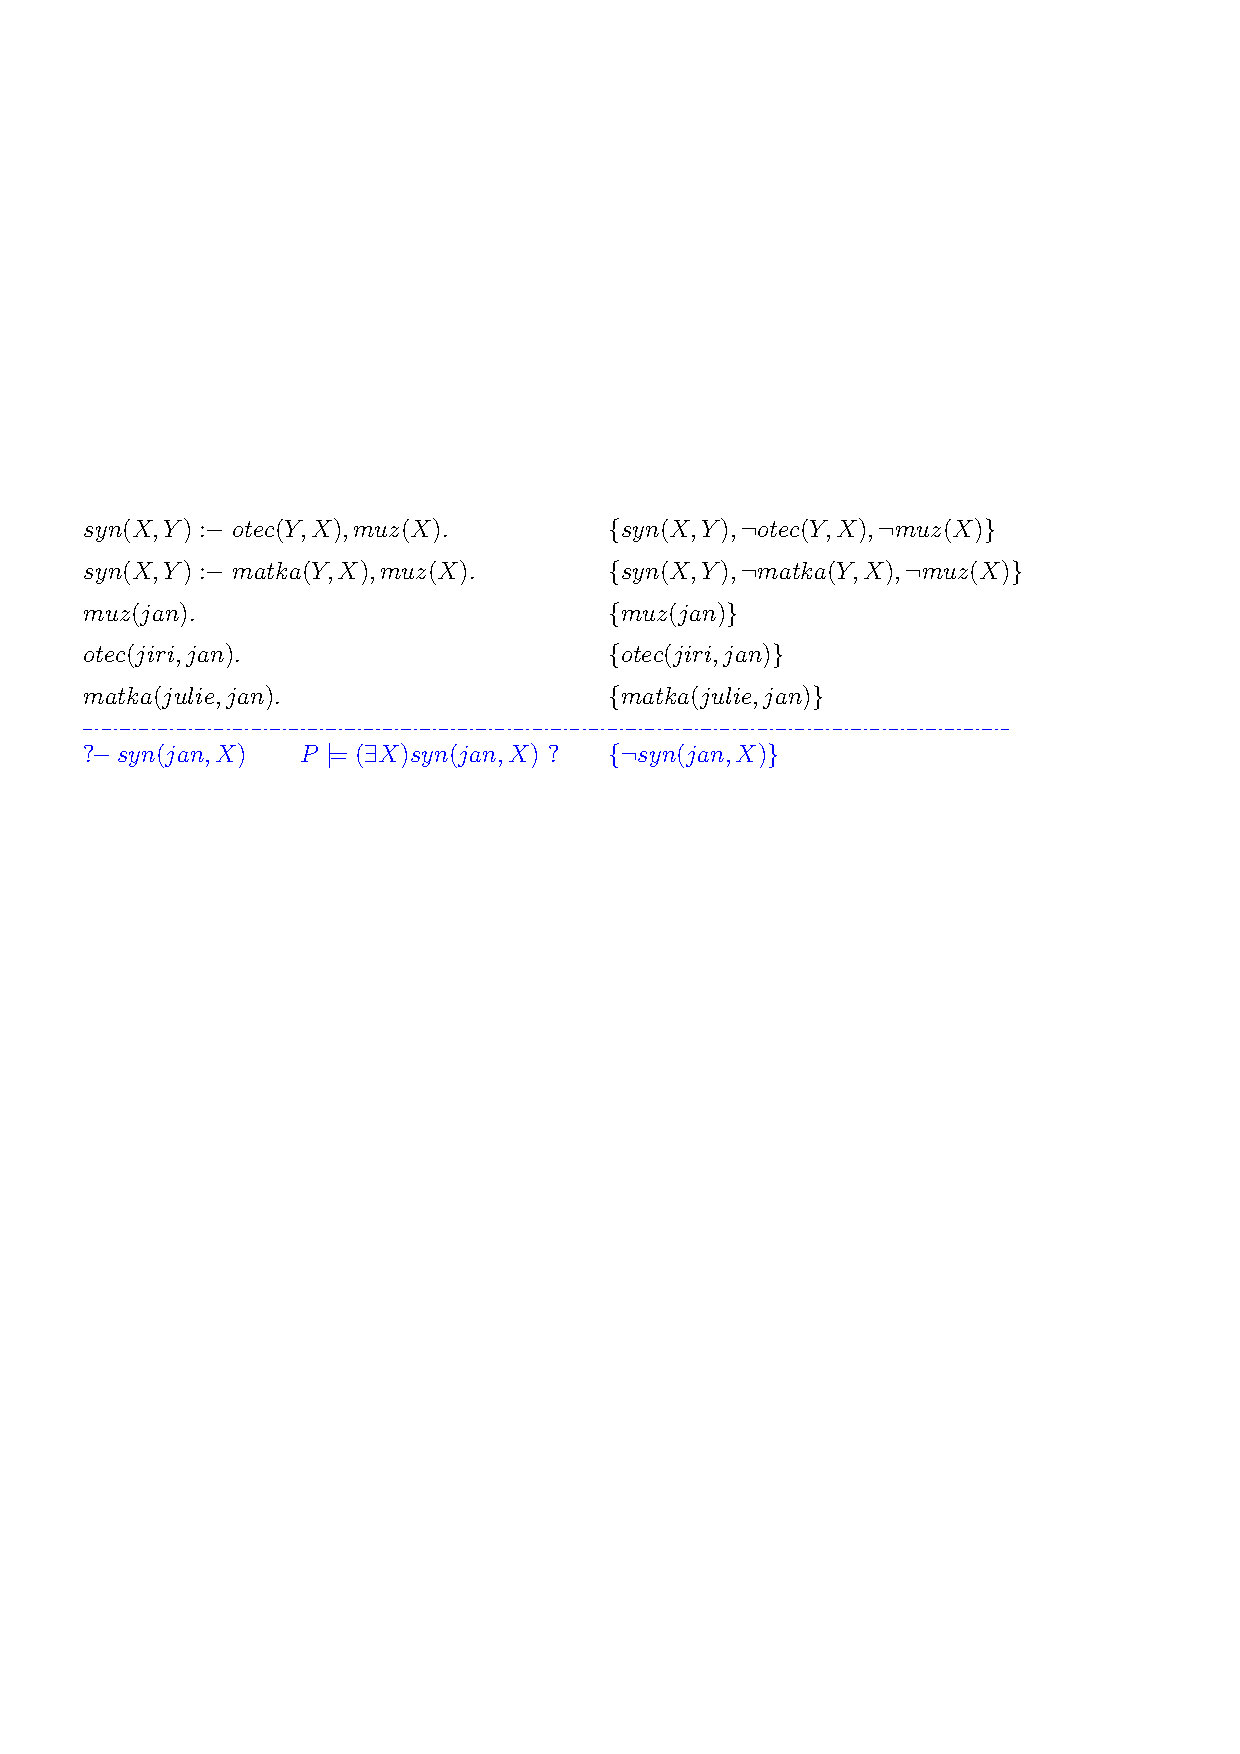
\includegraphics[scale=0.7]{files/rezolucePLprogram}}
    \bigskip
    
    {\it Zajímá nás, zda daný \myblue{existenční dotaz} vyplývá z daného programu.}%, navíc to chceme doložit \myblue{výstupní substitucí}.
    \medskip
    
    {\bf \myblue{Důsledek}}\ \ {\it Pro program $P$ a cíl $G=\{\neg A_1, \dots, \neg A_n\}$ v proměnných $X_1,\dots,X_m$
    
    \vspace{-0mm}
    \begin{enumerate}
    \item[$(1)$] $P \models (\exists X_1)\dots(\exists X_m)(A_1\mand \dots \mand A_n)$, právě když
    \smallskip
    
    \item[$(2)$] $\square$ lze odvodit LI-rezolucí z $P\cup\{G\}$ začínající (variantou) cíle $G$.
    \end{enumerate}}
    
    
    %%%%%%%%%%%%%%%%%%%%%%%%%%%%%%%%%%%%%%%%%%%%%%%%%%%%%%5
    
    \subsubsection*{LI-rezoluce nad programem}
    {\it Je-li odpověď na dotaz kladná, chceme navíc znát výstupní substituci.}
    \medskip
    
    \mdef{Výstupní substituce} $\sigma$ LI-rezoluce $\square$ z $P\cup\{G\}$ začínající $G=\{\neg A_1,\dots,\neg A_n\}$
    \smallskip
    
    je složení \myblue{mgu} v jednotlivých krocích (jen na proměnné v $G$). Platí,
    \vspace{-2mm}
    \mygreen{$$P \models (A_1 \mand \dots \mand A_n)\sigma.$$}
    
    \vspace{-2mm}
    
    \centerline{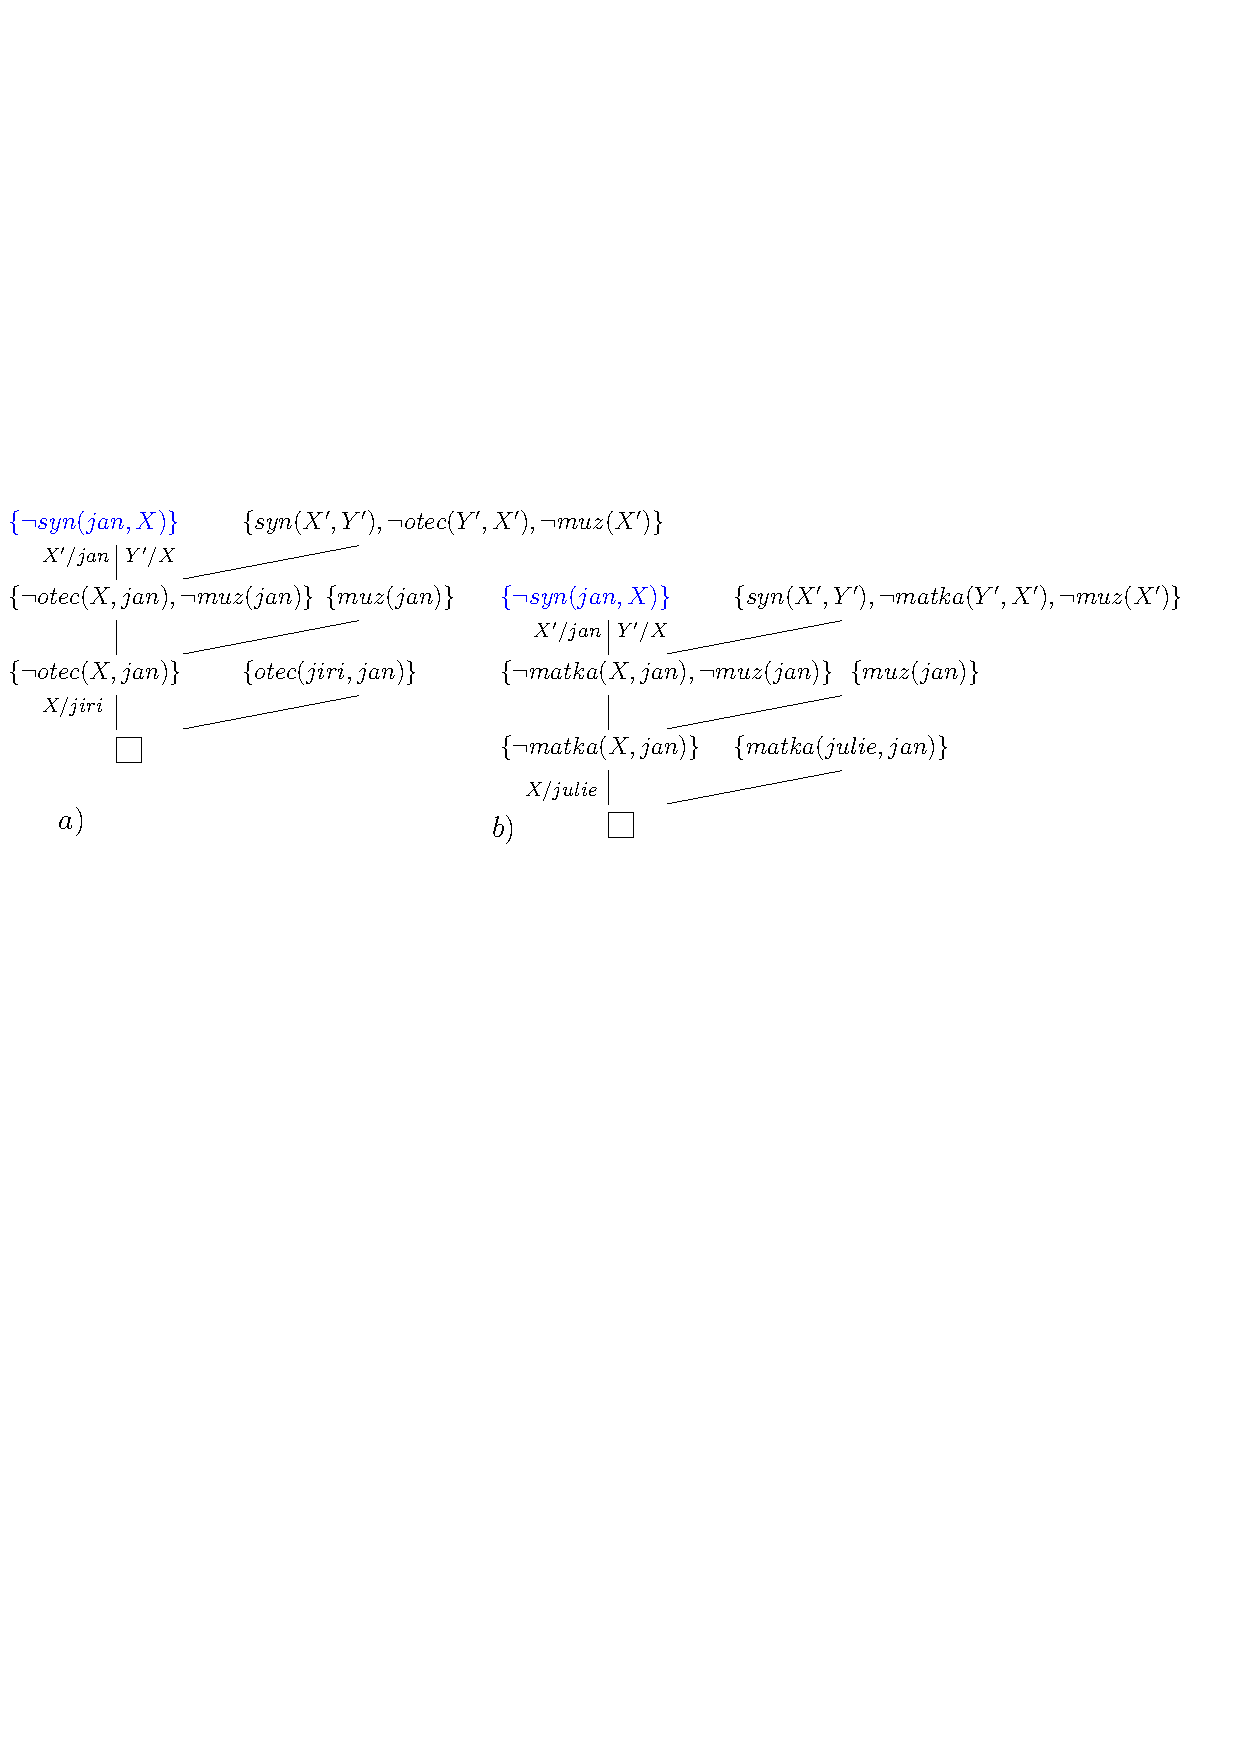
\includegraphics[scale=0.63]{files/rezolucePLprogramLI}}
    \bigskip
    
    Výstupní substituce $a)$ $X=jiri$,\ \ $b)$ $X=julie$.
    
    
% :from slides





% \part{Pokročilé partie}

% \chapter{Teorie modelů}\label{chapter:model-theory}

V této kapitole se trochu vzdálíme typickým aplikacím logiky v informatice\footnote{Například použití rezoluce k řešení otázky, zda v dané konečné teorii $T$ platí daná sentence $\varphi$.} a nahlédneme o úroveň abstrakce výše, do oblasti \emph{matematické} logiky. \emph{Teorie modelů} se snaží popsat vztah mezi obecnými vlastnostmi teorií (predikátové logiky) a tříd jejich modelů. Nevyhneme se práci s nekonečnými teoriemi a s nekonečnými strukturami. Jde jen o ukázku několika vybraných výsledků, které jsou pro nás dostupné. Ani se nepokusíme obsáhnout všechny hlavní oblasti teorie modelů, která je velmi bohatá a hluboká. Do této kapitoly jsme také přidali materiál týkající se vlastností modelů, který se nehodil jinam.


\section{Elementární ekvivalence}

Nejprve se podíváme na několik vlastností souvisejících s pojmem \emph{elementární ekvivalence}. Připomeňme, že $L$-struktury $\A$ a $\B$ jsou \emph{elementárně ekvivalentní} ($\A\equiv \B$), pokud v nich platí tytéž $L$-sentence.

V teorii modelů nás často zajímá, jaké vlastnosti (sentence) platí v dané, konkrétní struktuře:

\begin{definition}[Teorie struktury]
Mějme $L$-strukturu $\A$. \emph{Teorie struktury} $\A$, značíme $\Th(\A)$ je množina všech $L$-sentencí platných v $\A$:
$$
\Th(\A)=\{\varphi\mid\varphi\text{ je $L$-sentence a }\A\models\varphi\}
$$
\end{definition}

\begin{example}
Jako důležitý příklad vezměme \emph{standardní model aritmetiky}, strukturu $\underline{\mathbb{N}}=\langle\mathbb{N},S,+,\cdot,0,\le\rangle$. Teorii $\Th(\underline{\mathbb{N}})$ říkáme \emph{aritmetika přirozených čísel}. V následující kapitole si ukážeme, že je \emph{(algoritmicky) nerozhodnutelná}.\footnote{Teorie $T$ je \emph{(algoritmicky) rozhodnutelná}, pokud existuje algoritmus, který pro každou vstupní sentenci $\varphi$ doběhne a odpoví, zda $T\models\varphi$.}
\end{example}

Několik jednoduchých vlastností teorie struktury shrneme v následujícím pozorování:

\begin{observation}
    Nechť $\A$ je $L$-struktura a $T$ je $L$-teorie. Potom:
    \begin{enumerate}[(i)]
        \item Teorie $\Th(\A)$ je kompletní.
        \item Je-li $\A\in\M_L(T)$, potom $\Th(\A)$ je (kompletní) jednoduchá extenze teorie $T$.
        \item Pokud $\A\in\M_L(T)$ a $T$ je kompletní, potom je $\Th(\A)$ ekvivalentní s $T$, v tom případě $\Th(\A)=\Conseq_L(T)$.
    \end{enumerate}    
\end{observation}

Pomocí pojmu \emph{teorie struktury} můžeme také vyjádřit elementární ekvivalenci, pro $L$-struktury $\A,\B$ platí:
$$
\A\equiv\B \text{ právě když }\Th(\A)=\Th(\B).
$$

\begin{example}
   Podívejme se standardní uspořádání reálných, racionálních, a celých čísel, tj. na struktury $\langle\mathbb R,\leq\rangle$, $\langle\mathbb Q,\leq\rangle$, $\langle\mathbb Z,\leq\rangle$. Jak jsme již zmínili v Příkladu \ref{example:elementary-equivalence-of-orders-R-Q}, není těžké ukázat, že $\langle\mathbb R,\leq\rangle\equiv\langle\mathbb Q,\leq\rangle$ (pomocí \emph{hustoty} těchto uspořádání). Struktury $\langle\mathbb Q,\leq\rangle$ a $\langle\mathbb Z,\leq\rangle$ ale elementárně ekvivalentní nejsou: V $\langle\mathbb Z,\leq\rangle$ má každý prvek bezprostředního následníka, což v $\langle\mathbb Q,\leq\rangle$ neplatí. Pro následující sentenci $\varphi$ tedy máme $\varphi\in\Th(\langle\mathbb Z,\leq\rangle)$ ale $\varphi\not\in\Th(\langle\mathbb Q,\leq\rangle)$:
   $$
   \varphi=(\forall x)(\exists y)(x\leq y\land \neg x=y\land(\forall z)(x\leq z\limplies z=x\lor y\leq z))
   $$
\end{example}


\subsection{Kompletní jednoduché extenze}

Máme-li teorii $T$, zajímá nás, jak vypadají její modely. Připomeňme, že:
\begin{itemize}
    \item Teorie je \emph{kompletní}, právě když má jediný model až na elementární ekvivalenci.\footnote{Tedy všechny její modely jsou elementárně ekvivalentní.}
    \item Modely teorie $T$, až na elementární ekvivalenci, jednoznačně odpovídají kompletním jednoduchým extenzím $T$, až na ekvivalenci.
\end{itemize}
Kompletní jednoduché extenze $L$-teorie $T$ jsou tedy (až na ekvivalenci) tvaru $\Th(\A)$ pro $\A\in\M_L(T)$, a (jak jsme už zmínili výše) $\A\equiv\B$ právě když $\Th(\A)=\Th(\B)$. Místo hledání všech modelů tedy stačí najít všechny kompletní jednoduché extenze.

\begin{remark}
    Jednou z motivací, proč se zabývat kompletními jednoduchými extenzemi, je Tvrzení \ref{propositon:recursively-enumerable-completion} z následující kapitoly, které říká, že pokud lze \emph{efektivně (algoritmicky) popsat} všechny kompletní jednoduché extenze\footnote{Představte si algoritmus, který pro daná vstupní $i,j$ odpoví $j$-tý axiom $i$-té kompletní jednoduché extenze (v nějakém pevném očíslování); takový algoritmus ne vždy existuje!} \emph{efektivně dané} teorie $T$,\footnote{$T$ může být nekonečná, ale musí existovat algoritmus, který postupně vygeneruje všechny axiomy $T$.} potom je $T$ \emph{(algoritmicky) rozhodnutelná}.
\end{remark}


Schopnost (efektivně) popsat všechny kompletní jednoduché extenze je poměrně vzácná, a vyžaduje silné předpoklady. Přesto to lze provést u mnoha důležitých teorií. Uveďme jeden příklad: \emph{teorii hustého lineárního uspořádání (dense linear order)}.

\subsubsection{Příklad: DeLO*}

Teorie \emph{hustého lineárního uspořádání (DeLO*)}  je extenze teorie uspořádání o následující axiomy: 
\begin{itemize}
    \item axiom \emph{linearity} (někdy se mu říká také \emph{dichotomie}):
    $$
    x\leq y\lor y\leq x
    $$
    \item axiom \emph{hustoty}
    $$
    {x\leq y}\land{\neg\,x=y}\limplies(\exists z)(x\leq z\land z\leq y\land\neg\,z=x\land\neg\,z=y)
    $$
\end{itemize}
Někdy se přidává i axiom \emph{netriviality} $(\exists x)(\exists y)(\neg\,x=y)$ zakazující jednoprvkový model. Tato teorie není kompletní, umíme ale popsat všechny její kompletní jednoduché extenze:

\begin{proposition}
Mějme sentence $\varphi=(\exists x)(\forall y)(x\leq y)$ a $\psi=(\exists x)(\forall y)(y\leq x)$ vyjadřující existenci minimálního resp. maximálního prvku. Následující čtyři teorie jsou právě všechny (až na ekvivalenci) kompletní jednoduché extenze teorie DeLO*:
\begin{itemize}
    \item $\DeLO = \DeLO^*\ \cup \ \{\neg\varphi
    ,\neg\psi\}$
    \item $\DeLO^+ = \DeLO^*\ \cup \ \{\neg\varphi
    ,\psi\}$
    \item $\DeLO^- = \DeLO^*\ \cup \ \{\varphi
    ,\neg\psi\}$
    \item $\DeLO^\pm = \DeLO^*\ \cup \ \{\varphi
    ,\psi\}$        
\end{itemize}
\end{proposition}

Stačí ukázat, že tyto čtyři teorie jsou kompletní. Potom už je zřejmé, že žádná další kompletní jednoduchá extenze DeLO* nemůže existovat. Jak vysvětlíme v Sekci \ref{section:categoricity}, jejich kompletnost plyne z faktu, že jsou \emph{$\omega$-kategorické}, tj. mají jediný spočetný model až na \emph{izomorfismus}. Viz Důsledek \ref{corollary:complete-simple-extensions-of-delo}.


\subsection{Důsledky Löwenheim-Skolemovy věty}

V Sekci \ref{subsection:loewenheim-skolem-theorem} jsme dokázali tzv. Löwenheim-Skolemovu větu, konkrétně její variantu pro jazyky bez rovnosti:

\begin{theorem-unnumbered}[Löwenheim-Skolemova]
    Je-li $L$ spočetný jazyk bez rovnosti, potom každá bezesporná $L$-teorie má spočetně nekonečný model.
\end{theorem-unnumbered}

Tato věta má následující jednoduchý důsledek:

\begin{corollary}\label{corollary:loewenheim-skolem-without-equality}
    Je-li $L$ spočetný jazyk bez rovnosti, potom ke každé $L$-struktuře existuje elementárně ekvivalentní spočetně nekonečná struktura.
\end{corollary}
\begin{proof}
    Mějme $L$-strukturu $\A$. Teorie $\Th(\A)$ je bezesporná (má model $\A$), tedy dle Löwenheim-Skolemovy věty má spočetně nekonečný model $\B\models\Th(\A)$. To ale znamená, že $\B\equiv\A$.
\end{proof}
V jazyce bez rovnosti tedy nemůžeme vyjádřit například `model má právě 42 prvků'.

V důkazu Löwenheim-Skolemovy věty jsme sestrojený model získali jako kanonický model pro bezespornou větev tabla z $T$ pro položku $\F\bot$. Stejným způsobem se dokáže následující verze pro jazyky s rovností, stačí faktorizovat dle relace $=^A$:

\begin{theorem-unnumbered}[Löwenheim-Skolemova s rovností]
    Je-li $L$ spočetný jazyk s rovností, potom každá bezesporná $L$-teorie má spočetný model (tj. konečný, nebo spočetně nekonečný).
\end{theorem-unnumbered}

I tato verze má snadný důsledek pro konkrétní struktury:

\begin{corollary}\label{corollary:loewenheim-skolem-with-equality}
    Je-li $L$ spočetný jazyk s rovností, potom ke každé \emph{nekonečné} $L$-struktuře existuje elementárně ekvivalentní spočetně nekonečná struktura.
\end{corollary}
\begin{proof}
    Mějme nekonečnou $L$-strukturu $\A$. Stejně jako v důkazu Důsledku \ref{corollary:loewenheim-skolem-without-equality} (ale za použití Löwenheim-Skolemovy věty s rovností) najdeme spočetnou strukturu $\B\equiv\A$. Protože v $\A$ platí pro každé $n\in\mathbb N$ sentence vyjadřující `existuje alespoň $n$ prvků' (což lze pomocí rovnosti snadno zapsat), platí tato sentence i v $\B$, $\B$ tedy nemůže být konečná a musí být spočetně nekonečná.
\end{proof}

Tento důsledek použijeme, abychom ukázali, že existuje spočetné těleso, které je algebraicky uzavřené:  

\subsubsection*{Spočetné algebraicky uzavřené těleso}

Těleso $\A$ je \emph{algebraicky uzavřené}, pokud každý polynom nenulového stupně v něm má kořen. Těleso reálných čísel $\mathbb R$ není algebraicky uzavřené, neboť $x^2+1$ nemá v $\mathbb R$ kořen, stejně tak těleso $\mathbb Q$ (v něm nemá kořen ani $x^2-2$). Těleso komplexních čísel $\mathbb C$ algebraicky uzavřené je, je ale nespočetné.

Algebraickou uzavřenost lze vyjádřit pomocí následujících sentencí $\psi_n$, pro každé $n>0$:
$$
(\forall x_{n-1})\dots(\forall x_0)(\exists y)(y^n+x_{n-1}\cdot y^{n-1}+\dots+x_1\cdot y + x_0) = 0
$$
kde $y^k$ je zkratka za term $y\cdot y \cdot\ \cdots\ \cdot y$ (kde  $\cdot$ je aplikováno ($k-1$)-krát).

\begin{corollary}
    Existuje spočetné algebraicky uzavřené těleso.
\end{corollary}
\begin{proof}
    Dle Důsledku \ref{corollary:loewenheim-skolem-with-equality} existuje spočetně nekonečná struktura $\A$ elementárně ekvivalentní tělesu $\mathbb C$. Protože $\mathbb C$ je těleso a splňuje sentence $\psi_n$ pro všechna $n>0$, je i $\A$ algebraicky uzavřené těleso.
\end{proof}


\section{Izomorfismus struktur}\label{section:isomorphism-of-structures}

Podívejme se blíže na pojem \emph{izomorfismu struktur}, který zobecňuje izomorfismus grafů, vektorových prostorů, apod. Neformálně řečeno, struktury jsou \emph{izomorfní}, pokud se liší jen pojmenováním konkrétních prvků.

\begin{definition}
Mějme struktury $\A,\B$ jazyka $L=\langle\mathcal R,\mathcal F\rangle$. \emph{Izomorfismus $\A$ a $\B$} (nebo `$\A$ \emph{na} $\B$') je bijekce $h\colon A\to B$ splňující následující vlastnosti:
\begin{itemize}
    \item Pro každý ($n$-ární) funkční symbol $f\in\mathcal F$ a pro všechna $a_i\in A$ platí:
    $$
    h(f^\A(a_1,\dots,a_n))=f^\B(h(a_1),\dots,h(a_n))
    $$
    (Speciálně, je-li $c\in\mathcal F$ konstantní symbol, platí $h(c^\A)=c^\B$.)
    \item Pro každý ($n$-ární) relační symbol $R\in\mathcal R$ a pro všechna $a_i\in A$ platí:
    $$
    R^\A(a_1,\dots,a_n)\ \text{ právě když }\ R^\B(h(a_1),\dots,h(a_n))
    $$
\end{itemize}
Pokud existuje, říkáme, že $\A$ a $\B$ jsou \emph{izomorfní} (nebo `$\A$ je \emph{izomorfní s $\B$ via $h$}') a píšeme $\A\simeq\B$ (nebo $\A\simeq_h\B$). \emph{Automorfismus} $\A$ je izomorfismus $\A$ na $\A$.
\end{definition}

Všimněte si, že relace `býti izomorfní' je ekvivalence. Ukažme si jeden příklad:

\begin{example}
    Je-li $|X|=n$, je potenční algebra $\underline{\mathcal P(X)}=\langle \mathcal P(X),-,\cap,\cup,\emptyset,X\rangle$ izomorfní s Booleovou algebrou  $\underline{2^n}=\langle \{0,1\}^n,-_n,\land_n,\lor_n,(0,\dots,0),(1,\dots,1)\rangle$ (kde operace aplikujeme po složkách) via $h(A)=\chi_A$, kde $\chi_A$ je charakteristický vektor podmnožiny $A\subseteq X$.
\end{example}

Nyní ukážeme, že izomorfismus je bijekce `zachovávající sémantiku':

\begin{proposition}
Mějme struktury $\A,\B$ jazyka $L=\langle\mathcal R,\mathcal F\rangle$. Bijekce $h\colon A\to B$ je izomorfismus $\A$ a $\B$, právě když platí následující:
\begin{enumerate}[(i)]
    \item pro každý $L$-term $t$ a ohodnocení proměnných $e:\Var\to A$:
    $$
    h(t^\A[e])=t^\B[e\circ h]
    $$
    \item pro každou $L$-formuli $\varphi$ a ohodnocení proměnných $e:\Var\to A$:
    $$
    \A\models \varphi[e]\ \text{ právě když }\ \B\models\varphi[e\circ h]
    $$
\end{enumerate}
\end{proposition}
\begin{proof}
    Je-li $h$ izomorfismus, vlastnosti snadno dokážeme indukcí podle struktury termu resp. formule. Naopak, je-li $h$ bijekce splňující (i) a (ii), dosazením $t=f(x_1,\dots,x_n)$ resp. $\varphi=R(x_1,\dots,x_n)$ dostáváme vlastnosti z definice izomorfismu.
\end{proof}

Jako okamžitý důsledek dostáváme fakt, že izomorfní struktury jsou elementárně ekvivalentní:

\begin{corollary}\label{corollary:isomorphic-implies-elementarily-equivalent}
    Pokud $\A\simeq\B$, potom $\A\equiv\B$.
\end{corollary}

\begin{remark}
    Obrácená implikace ale obecně neplatí, například pro uspořádané množiny racionálních a reálných čísel platí $\langle\mathbb Q,\leq \rangle\equiv\langle\mathbb R,\leq\rangle$ ale $\langle\mathbb Q,\leq \rangle\not\simeq \langle \mathbb R,\leq\rangle$ neboť $\mathbb Q$ je spočetná množina zatímco $\mathbb R$ není (neexistuje tedy mezi nimi žádná bijekce).
\end{remark}

Pro konečné modely ale platí, že izomorfismus je totéž co elementární ekvivalence, máme-li jazyk s rovností, jak dokážeme v následujícím tvrzení:

\begin{proposition}
    Je-li $L$ jazyk s rovností a $\A,\B$ konečné $L$-struktury, potom platí:
    $$
    \A\simeq\B\ \text{ právě když }\ \A\equiv\B
    $$
\end{proposition}
\begin{proof}
    Jednu implikaci jsme dokázali v Důsledku \ref{corollary:isomorphic-implies-elementarily-equivalent}. Předpokládejme, že $\A\equiv\B$ a ukažme, že existuje izomorfismus $\A$ na $\B$. Protože je jazyk s rovností, můžeme vyjádřit sentencí, že `existuje právě $n$ prvků'. Z toho plyne, že $|A|=|B|$.

    Označme jako $\A'$ expanzi $\A$ o jména prvků z $A$; jde o strukturu v jazyce $L'=L\cup\{c_a\mid a\in A\}$. Ukážeme, že $\B$ lze expandovat na $L'$-strukturu $\B$ tak, že $\A'\equiv \B'$. Potom, jak lze snadno ověřit, je zobrazení $h(a)= c_a^{\B'}$ izomorfismem $\A'$ na $\B'$, a tedy i izomorfismem jejich $L$-reduktů a $\A\simeq\B$.

    Stačí ukázat, že pro každé $c_a^{\A'}=a\in A$ existuje prvek $b\in B$ takový, že pro expanze o interpretaci konstantního symbolu $c_a$ platí $\langle  \A,a\rangle\equiv\langle\B,b\rangle$. Označme jako $\Omega$ množinu formulí $\varphi(x)$ takových, že $\langle \A,a\rangle \models \varphi(x/c_a)$, neboli $\A\models \varphi[e(x/a)]$. Protože je $A$ konečná množina, existuje konečně mnoho formulí $\varphi_1(x),\dots,\varphi_m(x)$ takových, že pro každou formuli $\varphi \in \Omega$ existuje $i$ takové, že $\A\models \varphi\liff\varphi_i$. Potom i $\B\models\varphi\liff\varphi_i$ (neboť $\A\equiv\B$, stačí vzít generální uzávěr této formule, což je sentence).
    
    Protože v $\A$ platí sentence $(\exists x)\bigwedge_{i=1}^m\varphi_i$ (je splněna díky prvku $a\in A$) a $\B\equiv\A$, máme i $\B\models (\exists x)\bigwedge_{i=1}^m\varphi_i$. Jinými slovy, existuje $b\in B$ takové, že $\B\models\bigwedge_{i=1}^m\varphi_i[e(x/b)]$. Tedy pro každou $\varphi\in \Omega$ platí $\B\models \varphi[e(x/b)]$, tj. $\langle\mathcal{B},b\rangle\models \varphi(x/c_a)$, což jsme chtěli dokázat.
\end{proof}

\begin{corollary}
    Pokud má kompletní teorie v jazyce s rovností konečný model, potom jsou všechny její modely izomorfní.
\end{corollary}


\subsection{Definovatelnost a automorfismy}

Připomeňme si pojem definovatelné množiny, viz Sekce \ref{section:definability}. Ukážeme si užitečnou vlastnost definovatelných množin: jsou uzavřené (`invariantní') na automorfismy dané struktury. 

Nikoho nepřekvapí, že při automorfismu se musí izolovaný vrchol daného grafu zobrazit na izolovaný vrchol, vrchol stupně 4 na vrchol stejného stupně, nebo třeba trojice vrcholů, která tvoří trojúhelník, na trojúhelník. To nám může pomoci například při hledání automorfismů.

\begin{proposition}
    Je-li $D\subseteq A^n$ definovatelná ve struktuře $\A$, potom pro každý automorfismus $h\in\Aut(\A)$ platí $h[D]=D$ (kde $h[D]$ značí $\{(h(\overline{a})\mid\overline{a}\in D\}$).

    Je-li $D$ definovatelná s parametry $\overline{b}$, platí totéž pro automorfismy identické na $\overline{b}$ (\emph{fixující} $\overline{b}$), tj. takové, že $h(\overline{b})=\overline{b}$ (neboli $h(b_i)=b_i$ pro všechna $i$).
\end{proposition}
\begin{proof}
    Ukážeme jen verzi s parametry. Nechť $D=\varphi^{\A,\overline{b}}(\overline{x},\overline{y})$. Potom pro každé $\overline{a}\in A^n$ platí následující ekvivalence:
\begin{align*}
\overline{a}\in D\ 
&\Leftrightarrow\ \A\models \varphi[e(\overline{x}/\overline{a},\overline{y}/\overline{b})]\\
&\Leftrightarrow\  \A\models \varphi[(e\circ h)(\overline{x}/\overline{a},\overline{y}/\overline{b})]\\
&\Leftrightarrow\ \A\models \varphi[e(\overline{x}/h(\overline{a}),\overline{y}/h(\overline{b}))]\\
&\Leftrightarrow\ \A\models \varphi[e(\overline{x}/h(\overline{a}),\overline{y}/\overline{b})]\\
&\Leftrightarrow\ h(\overline{a})\in D.
\end{align*}
\end{proof}

\begin{example}
    Uvažme následující graf $\mathcal G$. Najděme všechny množiny definovatelné z $\mathcal G$ s parametrem $0$, tj. množinu 
    $\mathrm{Df}^1(\mathcal G,\{0\})$. 
    \begin{center}
        \begin{tikzpicture}[every node/.style={circle,fill=blue!10,draw,minimum size=0.5cm,node distance=1.5cm}]
            \node (1) {$1$};
            \node[below left of=1](0) {$0$};
            \node[below right of=0] (4) {$4$};
            \node[right of=4] (3) {$2$};
            \node[right of=1] (2) {$3$};
            \path[draw] (0) -- (1) -- (2) -- (3) -- (4) -- (0);
        \end{tikzpicture}
    \end{center}
    Tento graf má jediný netriviální automorfismus zachovávající vrchol $0$: $h(i)=(5-i) \bmod 5$. Jeho \emph{orbity} jsou $\{0\}$, $\{1,4\}$, a $\{2,3\}$. Tyto množiny jsou definovatelné:
    \begin{itemize}
        \item $\{0\}$ je definované formulí $x=y$, tj. $(x=y)^{\mathcal G,\{0\}}=\{0\}$,
        \item $\{1,4\}$ lze definovat pomocí formule $E(x,y)$, a
        \item $\{2,3\}$ formulí $\neg E(x,y)\land \neg x=y$.
    \end{itemize}
    Množina $\mathrm{Df}^1(\mathcal G,\{0\})$ je podalgebra potenční algebry $\underline{\mathcal P(V(\mathcal G))}$, musí tedy být uzavřená na doplněk, sjednocení, průnik, a obsahovat $\emptyset$ a $V(\mathcal G)$. Podalgebra generovaná $\{\{0\},\{1,4\},\{2,3\}\}$ už ale obsahuje všechny podmnožiny zachovávající automorfismus $h$. Dostáváme:
    $$
    \mathrm{Df}^1(\mathcal G,\{0\})=\{\emptyset, \{0\}, \{1,4\}, \{2,3\}, \{0,1,4\}, \{0,2,3\}, \{1,4,2,3\}, \{0,1,2,3,4\}\}
    $$
\end{example}

\begin{exercise}
    Uvažme následující graf. Najděte všechny automorfismy. Určete, které podmnožiny jsou definovatelné, uveďte definující formule. Které binární relace jsou definovatelné?
    \begin{center}
        \begin{tikzpicture}[every node/.style={circle,fill=blue!10,draw,minimum size=0.5cm,node distance=1.5cm}]
            \node (1) {$1$};
            \node[right of=1] (2) {$2$};
            \node[below of=2] (3) {$3$};
            \node[left of=3] (4) {$4$};
            \path[draw] (1) -- (2) -- (3) -- (4) -- (1) -- (3);
            \node[right of=3] (5) {$5$};
            \path[draw] (2) -- (5) -- (3);
        \end{tikzpicture}
    \end{center}
\end{exercise}


\section{$\omega$-kategorické teorie}\label{section:categoricity}

Nyní se podíváme na teorie, které mají jediný spočetně nekonečný model (až na izomorfismus), říkáme jim \emph{$\omega$-kategorické}.\footnote{Symbol $\omega$ se používá pro nejmenší nekonečné \emph{ordinální} číslo, jinými slovy, pro množinu všech přirozených čísel.}

\begin{definition}[Izomorfní spektrum, $\kappa$-kategoricita]
    \emph{Izomorfní spektrum} teorie $T$ je počet $
    I(\kappa,T)$ modelů $T$ kardinality $\kappa$ až na izomorfismus, pro každou kardinalitu $\kappa$ (včetně \emph{transfinitních}).     Teorie $T$ je \emph{$\kappa$-kategorická}, pokud $
    I(\kappa,T)=1$.
\end{definition}

Nadále nás bude zajímat jen případ $\kappa=\omega$, totiž teorie s jediným spočetně nekonečným modelem (až na izomorfismus). Jako příklad uveďme teorii hustého lineárního uspořádání bez konců:

\begin{proposition}
    Teorie DeLO je $\omega$-kategorická.
\end{proposition}
\begin{proof}
Vezměme dva spočetně nekonečné modely $\A,\B$ a očíslujme jejich prvky: $A=\{a_i\mid i\in\mathbb N\}$, $B=\{b_i\mid i\in\mathbb N\}$. Indukcí podle $n$ lze díky hustotě nalézt posloupnost $h_0\subseteq h_1\subseteq h_2\subseteq\dots$ prostých (parciálních) funkcí z $A$ do $B$, takových, že $\{a_0,\dots,a_{n-1}\}\subseteq\dom h_n$, $\{b_0,\dots,b_{n-1}\}\subseteq\rng h_n$,\footnote{Zde $\dom$ značí \emph{doménu} a $\rng$ značí \emph{obor hodnot (`range')} funkce.} a \emph{zachovávají uspořádání}\footnote{Tj. je-li $a_i,a_j\in\dom h_n$, potom $a_i\leq^\A a_j$ právě když $h(a_i)\leq^\B h(a_j)$.} Potom $\A\simeq\B$ via $h=\bigcup_{n\in\mathbb N}h_n$.
\end{proof}

\begin{corollary}
Izomorfní spektrum teorie DeLO* je následující:
$$
I(\kappa,DeLO^*)=\begin{cases}
    0 &\text{pro }\kappa\in\mathbb{N},\\
    4 &\text{pro }\kappa=\omega.
\end{cases}
$$
Spočetné modely až na izomorfismus jsou například:
$$ 
\mathbb Q=\langle \mathbb Q,\leq\rangle\simeq\mathbb Q\upharpoonright(0,1), \ \mathbb Q\upharpoonright(0,1], \ \mathbb Q \upharpoonright [0,1), \ \mathbb Q \upharpoonright [0,1]
$$
\end{corollary}

\begin{proof}
Husté uspořádání jistě nemůže být konečné. Izomorfismus musí zobrazit nejmenší prvek na nejmenší prvek, a největší na největší.
\end{proof}

Pojem \emph{$\omega$-kategoricity} lze chápat jako zeslabení pojmu \emph{kompletnosti}. Platí následující užitečné kritérium:

\begin{theorem}[$\omega$-kategorické kritérium kompletnosti]
Mějme $\omega$-kategorickou teorii $T$ ve spočetném jazyce $L$. Je-li
\begin{itemize}
    \item $L$ bez rovnosti, nebo
    \item $L$ s rovností a $T$ nemá konečné modely,
\end{itemize}
potom je teorie $T$ kompletní.
\end{theorem}
\begin{proof}
Pro jazyk bez rovnosti víme z Důsledku \ref{corollary:loewenheim-skolem-without-equality} Löwenheim-Skolemovy věty, že každý model je elementárně ekvivalentní nějakému spočetně nekonečnému modelu. Ten je ale až na izomorfismus jediný, takže všechny modely jsou elementárně ekvivalentní, což je sémantická definice kompletnosti.

Máme-li jazyk s rovností, použijeme podobně Důsledek \ref{corollary:loewenheim-skolem-with-equality} a dostaneme, že všechny nekonečné modely jsou elementárně ekvivalentní. Mohly by existovat elementárně neekvivalentní konečné modely, to jsme ale zakázali.
\end{proof}

\begin{corollary}\label{corollary:complete-simple-extensions-of-delo}
    Teorie $\DeLO$, $\DeLO^+$, $\DeLO^-$, a $\DeLO^\pm$ jsou kompletní. Jsou to všechny (navzájem neekvivalentní) kompletní jednoduché extenze teorie $DeLO^*$.
\end{corollary}

\begin{remark}
Analogické kritérium platí i pro kardinality $\kappa$ větší než $\omega$.
\end{remark}


\section{Axiomatizovatelnost}\label{section:axiomatizability}

Na závěr této kapitoly se podíváme, za jakých okolností lze `popsat' (\emph{axiomatizovat}) třídu modelů respektive teorii. Zajímat nás bude také kdy si vystačíme s konečně mnoha axiomy, a kdy to lze pomocí otevřených axiomů (kterých může být i nekonečně mnoho). Srovnejte s Tvrzením \ref{proposition:axiomatize-in-DNF-CNF} z výrokové logiky. 

\begin{definition}[Axiomatizovatelnost]
Mějme třídu struktur $K\subseteq\M_L$ v nějakém jazyce $L$. Říkáme, že $K$ je
\begin{itemize}
    \item \emph{axiomatizovatelná}, pokud existuje $L$-teorie $T$ taková, že $\M_L(T)=K$,
    \item \emph{konečně axiomatizovatelná}, pokud je axiomatizovatelná konečnou teorií, a
    \item \emph{otevřeně axiomatizovatelná}, pokud je axiomatizovatelná otevřenou teorií.
\end{itemize}
O $L$-teorii $T'$ říkáme, že je \emph{konečně} resp. \emph{otevřeně axiomatizovatelná}, pokud to platí o třídě modelů $K=\M_L(T')$.
\end{definition}

\begin{example}
    Uveďme několik příkladů:
    \begin{itemize}
        \item grafy nebo částečná uspořádání jsou konečně i otevřeně axiomatizovatelné,
        \item tělesa jsou konečně, ale ne otevřeně axiomatizovatelná,
        \item nekonečné grupy jsou axiomatizovatelné, ale ne konečně axiomatizovatelné,
        \item konečné grafy nejsou axiomatizovatelné.
    \end{itemize}
    Proč tomu tak je ukážeme níže.
\end{example}

Začněme jednoduchým faktem:

\begin{observation}
    Je-li $K$ axiomatizovatelná, musí být uzavřená na elementární ekvivalenci.  
\end{observation}

Z věty o kompaktnosti snadno získáme následující tvrzení, pomocí kterého lze ukázat neaxiomatizovatelnost např. konečných grafů, konečných grup, konečných těles.

\begin{theorem}
    Pokud má teorie libovolně velké konečné modely, potom má i nekonečný model. V tom případě není třída všech jejích konečných modelů axiomatizovatelná.
\end{theorem}
\begin{proof}
    Je-li jazyk bez rovnosti, stačí vzít kanonický model pro některou bezespornou větev v tablu z $T$ pro položku $\F\bot$ ($T$ je bezesporná, neboť má model(y), tedy tablo není sporné).     
    
    Mějme jazyk s rovností a označme jako $T'$ následující extenzi teorie $T$ do jazyka rozšířeného o spočetně mnoho nových konstantních symbolů $c_i$:
    $$
    T'=T \cup \{\neg c_i = c_j \mid i\neq j\in\mathbb N\}
    $$
    Každá konečná část teorie $T'$ má model: nechť $k$ je největší takové, že symbol $c_k$ se vyskytuje v této konečné části $T'$. Potom stačí vzít libovolný alespoň $(k+1)$-prvkový model $T$ a interpretovat konstanty $c_0,\dots,c_k$ jako navzájem různé prvky tohoto modelu.

    Dle věty o kompaktnosti má potom i $T'$ model. Ten je nutně nekonečný. Jeho redukt na původní jazyk (zapomenutí konstant $c_i^\A$) je nekonečným modelem $T$.
\end{proof}

\begin{remark}
    Třída všech \emph{nekonečných} modelů teorie ale je vždy axiomatizovatelná, máme-li jazyk s rovností: stačí k teorii přidat pro každé $n\in\mathbb N$ axiom vyjadřující `existuje alespoň $n$ prvků'.
\end{remark}


\subsection{Konečná axiomatizovatelnost}

Ukážeme následující kritérium konečné axiomatizovatelnosti: jak třída struktur $K$ tak i $\overline{K}$ musí být axiomatizovatelné.

\begin{theorem}[O konečné axiomatizovatelnosti]\label{theorem:finite-axiomatizability}
    Mějme třídu struktur $K\subseteq \M_L$ a uvažme také její doplněk $\overline{K}=\M_L\setminus K$. Potom $K$ je konečně axiomatizovatelná, právě když $K$ i $\overline{K}$ jsou axiomatizovatelné.   
\end{theorem}
\begin{proof}
Je-li $K$ konečně axiomatizovatelná, potom je axiomatizovatelná i konečně mnoha sentencemi $\varphi_1,\dots,\varphi_n$ (nahradíme formule jejich generálními uzávěry). Jako axiomatizaci $\overline{K}$ stačí vzít sentenci $\psi=\neg(\varphi_1\land\varphi_2\land\dots\land\varphi_n)$. Zřejmě platí $\M(\psi)=\overline{K}$.

Naopak, nechť $T$ a $S$ jsou teorie takové, že $\M(T)=K$ a $\M(S)=\overline{K}$. Uvažme teorii $T\cup S$. Tato teorie je sporná, neboť:
$$
\M(T\cup S)=\M(T)\cap \M(S)=K\cap\overline{K}=\emptyset
$$
Podle věty o kompaktnosti\footnote{Vidíte, jak je užitečná!} existují konečné podteorie $T'\subseteq T$ a $S'\subseteq S$ takové, že:
$$
\emptyset = \M(T'\cup S')=\M(T')\cap \M(S')
$$
Nyní si všimněme, že platí
$$
\M(T)\subseteq \M(T')\subseteq \overline{\M(S')}\subseteq \overline{\M(S)}=\M(T)
$$
tím jsme dokázali, že $M(T)=M(T')$, tj. teorie $T'$ je hledanou konečnou axiomatizací $K$.
\end{proof}

Jako aplikaci si dokážeme, že tělesa charakteristiky 0 nejsou konečně axiomatizovatelná.

\subsubsection*{Příklad: tělesa charakteristiky 0}
 
Nechť $T$ je teorie těles. Charakteristika tělesa je nejmenší počet jedniček, které je třeba sečíst, abychom dostali nulu (v tom případě musí být charakteristika prvočíslo---dokažte si!), nebo, pokud nikdy nedostaneme sčítáním jedniček nulu, říkáme že je charakteristika 0. Trochu formálněji:

\begin{definition}[Charakteristika tělesa]
Říkáme, že těleso $\A=\langle A,+,-,0,\cdot,1 \rangle$ je
\begin{itemize}
    \item \emph{charakteristiky $p$}, je-li $p$ nejmenší prvočíslo takové, že $\A\models p1=0$, kde $p1$ označuje term $1+1+\dots+1$ s $p$ jedničkami, nebo
    \item \emph{charakteristiky 0}, pokud není charakteristiky $p$ pro žádné prvočíslo $p$.
\end{itemize}
\end{definition}
Nechť $T$ je teorie těles. Potom třída těles charakteristiky $p$ je konečně axiomatizována teorií $T\cup \{p1=0\}$. Třída těles charakteristiky 0 je axiomatizována následující (nekonečnou) teorií:
$$
T'=T\cup \{\neg\, p1=0\mid p\text{ je prvočíslo}\}
$$
Konečná axiomatizace ale neexistuje.

\begin{proposition}
Třída $K$ těles charakteristiky $0$ není konečně axiomatizovatelná.   
\end{proposition}
\begin{proof}
Díky Větě \ref{theorem:finite-axiomatizability} stačí ukázat, že $\overline{K}$ (sestávající z těles nenulové charakteristiky a struktur, které nejsou tělesa) není axiomatizovatelná, což dokážeme sporem. Nechť existuje teorie $S$ taková, že $\M(S)=\overline{K}$. Potom teorie 
$S'=S\cup T'$ má model, neboť každá její konečná část má model: stačí vzít těleso prvočíselné charakteristiky větší než jakékoliv $p$ z axiomu $T'$ tvaru $\neg\, p1=0$. Nechť $\A$ je model $S'$. Potom je i $\A\in\M(S)=\overline{K}$. Zároveň je ale $\A\in\M(T')=K$, což je spor.
\end{proof}

\subsection{Otevřená axiomatizovatelnost}

Pro otevřenou axiomatizovatelnost existuje jednoduché sémantické kritérium: třída jejích modelů musí být uzavřená na podstruktury. Platí dokonce ekvivalence, dokážeme ale jen jednu implikaci (důkaz druhé je obtížnější).

\begin{theorem}\label{theorem:open-axiomatizability}
Pokud je teorie $T$ otevřeně axiomatizovatelná, potom je každá podstruktura modelu $T$ také modelem $T$.   
\end{theorem}

\begin{remark}
    Platí i obrácená implikace: Je-li každá podstruktura modelu $T$ také modelem, potom je $T$ otevřeně axiomatizovatelná. Důkaz zde ale neuvedeme.
\end{remark}

\begin{proof}
Nechť $T'$ je otevřená axiomatizace $T$. Mějme model $\A\models T'$  a podstrukturu $\B\subseteq\A$. Pro každou formuli $\varphi\in T'$ platí $\B\models\varphi$ (neboť $\varphi$ je otevřená), tedy i $\B\models T'$.  
\end{proof}

\begin{example}
    Uveďme několik příkladů:
    \begin{itemize}
        \item Teorie DeLO není otevřeně axiomatizovatelná, například žádná konečná podstruktura modelu DeLO nemůže být hustá.
        \item Teorie těles není otevřeně axiomatizovatelná, podstruktura $\mathbb Z\subseteq\mathbb Q$ tělesa racionálních čísel není tělesem, v $\mathbb Z$ neexistuje inverzní prvek vůči násobení k číslu $2$.
        \item Pro dané $n\in\mathbb N$ jsou nejvýše $n$-prvkové grupy otevřeně axiomatizovatelné(podgrupy jsou jistě také nejvýše $n$-prvkové). Jako otevřenou axiomatizaci lze vzít následující extenzi (otevřené) teorie grup $T$:
        $$
        T\cup \{\bigvee_{1\leq i<j\leq n+1}x_i=x_j\}
        $$
    \end{itemize}
\end{example}

% \chapter{Nerozhodnutelnost a neúplnost}

V této, závěrečné kapitole se budeme zabývat tím, jak lze s teoriemi pracovat algoritmicky. Zlatým hřebem budou \emph{Gödelovy věty o neúplnosti} z roku 1931, které ukazují limity formálního přístupu, a které zastavily desetiletí trvající program formalizace matematiky. Nemáme zde dostatek prostoru k uvedení formálních definic a úplných důkazů, proto se místy budeme pohybovat na poněkud intuitivní úrovni. Zaměříme se na pochopení smyslu tvrzení a myšlenek důkazů.

Pojem \emph{algoritmu} budeme chápat také jen intuitivně. Pokud bychom ho chtěli formalizovat, potom nejběžnější (ale zdaleka ne jedinou) volbou je koncept \emph{Turingova stroje}.\footnote{Viz přednáška NTIN090 Základy složitosti a vyčíslitelnosti.}

\section{Rekurzivní axiomatizace a rozhodnutelnost}

V dokazovacích systémech, kterými jsme se zabývali (tablo metoda, rezoluce, hilbertův kalkulus) jsme povolili, aby teorie $T$, ve které dokazujeme, byla nekonečná. Vůbec jsme se ale zatím nezabývali tím, jak je zadaná. Pokud chceme ověřit, že je daný objekt (tablo, rezoluční strom, posloupnost formulí) korektním důkazem, potřebujeme nějaký algoritmický přístup ke všem axiomům $T$. 

Jednou z možností by bylo požadovat \emph{enumerátor} $T$, tj. algoritmus, který vypisuje na výstup axiomy z $T$, a každý axiom někdy vypíše.\footnote{Nutným předpokladem je, aby $T$ byla spočetná. K tomu stačí předpokládat, že jazyk je spočetný.} Potom by bylo snadné potvrdit, že je daný důkaz korektní. Pokud bychom ale dostali důkaz, který použil chybný axiom, který v $T$ není, nikdy bychom se to nedozvěděli: nekonečně dlouho bychom čekali, zda jej enumerátor přeci jen nevypíše. Požadujeme proto silnější vlastnost, která umožňuje rozpoznat i chybné důkazy \emph{rekurzivní axiomatizaci}:\footnote{Slovo \emph{rekurzivní} zde neznamená běžně známou rekurzi, ale odkazuje na formalizaci algoritmu pomocí `rekurzivních funkcí' od Gödela. Rekurzivní funkce zde znamená totéž, co vyčíslitelná nějakým Turingovým strojem, a teorii vyčíslitelnosti (\emph{computability theory}) se někdy také říká \emph{recursion theory}.}

\begin{definition}[Rekurzivní axiomatizace]
    Teorie $T$ je \emph{rekurzivně axiomatizovaná}, pokud existuje algoritmus, který pro každou vstupní formuli $\varphi$ doběhne a odpoví, zda $\varphi\in T$.
\end{definition}

\begin{remark}
    Ve skutečnosti by nám stačil enumerátor pro $T$, pokud by bylo garantováno, že vypisuje axiomy v lexikografickém uspořádání. To už je ekvivalentní rekurzivní axiomatizaci. (Rozmyslete si proč.)
\end{remark}

Zaměříme se na otázku, zda můžeme v dané teorii $T$ `algoritmicky rozhodovat pravdu' (tj. platnost vstupní formule). Pokud ano, říkáme, že je teorie \emph{rozhodnutelná}. To je ale poměrně silná vlastnost, definujeme proto také \emph{částečnou rozhodnutelnost}, která znamená, že pokud formule platí, algoritmus nám to řekne, ale pokud neplatí, nikdy se nemusíme dočkat odpovědi.

\begin{definition}[Rozhodnutelnost]
O teorii $T$ říkáme, že je
\begin{itemize}
    \item \emph{rozhodnutelná}, pokud existuje algoritmus, který pro každou vstupní formuli $\varphi$ doběhne a odpoví, zda $T\models\varphi$,
    \item \emph{částečně rozhodnutelná}, pokud existuje algoritmus, který pro každou vstupní formuli:
    \begin{itemize}
        \item pokud $T\models\varphi$, doběhne a odpoví ``ano'',
        \item pokud $T\not\models\varphi$, buď nedoběhne, nebo doběhne a odpoví ``ne''.
    \end{itemize}
\end{itemize}
\end{definition}
Můžeme jako obvykle předpokládat, že $\varphi$ v definici je sentence. Ukážeme si jednoduché tvrzení:

\begin{proposition}
    Nechť $T$ je rekurzivně axiomatizovaná. Potom:
    \begin{enumerate}[(i)]
        \item $T$ je částečně rozhodnutelná,
        \item je-li $T$ navíc kompletní, potom je rozhodnutelná.
    \end{enumerate}
\end{proposition}
\begin{proof}
Algoritmem ukazujícím částečnou rozhodnutelnost je konstrukce systematického tabla pro $\F\varphi$.\footnote{Zde nám stačí enumerátor axiomů $T$, nebo postupně generujeme všechny sentence (např. v lexikografickém pořadí) a pro každou testujeme, zda je axiomem.} Pokud $\varphi$ v $T$ platí, konstrukce skončí v konečně mnoha krocích a snadno ověříme, že je tablo sporné, jinak ale skončit nemusí.

Je-li $T$ kompletní, víme, že platí právě jedna z následujících možností: buď $T\proves\varphi$ nebo $T\proves\neg\varphi$. Budeme tedy paralelně konstruovat tablo pro $\F\varphi$ a tablo pro $\T\varphi$ (důkaz a zamítnutí $\varphi$ z $T$): jedna z konstrukcí po konečně mnoha krocích skončí.
\end{proof}


\subsection{Rekurzivně spočetná kompletace}

Požadavek kompletnosti je příliš silný, ukážeme, že stačí pokud jsme schopni efektivně popsat všechny kompletní jednoduché extenze.\footnote{Tj. `všechny modely až na elementární ekvivalenci'.}

\begin{definition}[Rekurzivně spočetná kompletace]
Řekneme, že teorie $T$ má \emph{rekurzivně spočetnou kompletaci}, pokud (nějaká) množina až na ekvivalenci všech jednoduchých kompletních extenzí teorie $T$ je \emph{rekurzivně spočetná}, tj. existuje algoritmus, který pro danou vstupní dvojici přirozených čísel $(i,j)$ vypíše na výstup $i$-tý axiom $j$-té extenze (v nějakém pevně daném uspořádání\footnote{Zde potřebujeme, aby byl jazyk spočetný.}), nebo odpoví, že takový axiom už neexistuje.\footnote{Jeli extenzí méně než $j$, nebo má-li $j$-tá extenze méně než $i$ axiomů.}
\end{definition}

\begin{proposition}\label{propositon:recursively-enumerable-completion}    
    Pokud je teorie $T$ rekurzivně axiomatizovaná a má rekurzivně spočetnou kompletaci, potom je $T$ rozhodnutelná.
\end{proposition}
\begin{proof}
Pro danou sentenci $\varphi$ buď $T\proves\varphi$, nebo existuje protipříklad $\A\not\models\varphi$, tedy kompletní jednoduchá extenze $T_i$ teorie $T$ taková, že $T_i\not\proves\varphi$. Z kompletnosti ale plyne, že $T_i\proves\neg\varphi$. Náš algoritmus bude paralelně konstruovat tablo důkaz $\varphi$ z $T$ a (postupně) tablo důkazy $\neg\varphi$ ze všech kompletních jednoduchých extenzí $T_1,T_2,\dots$ teorie $T$.\footnote{Nevadí, že je jich nekonečně mnoho, můžeme využít tzv. \emph{dovetailing}: Provedeme 1. krok konstrukce 1. tabla, potom 2. krok 1. tabla a 1. krok 2. tabla, 3. krok 1. tabla, 2. krok 2. tabla, 1. krok 3. tabla, atd.} Víme, že alespoň jedno z paralelně konstruovaných tabel je sporné, a můžeme předpokládat, že konečné (neprodlužujeme-li sporné větve tabla), tedy algoritmus ho po konečně mnoha krocích zkonstruuje.
\end{proof}

\begin{exercise}
Ukažte, že následující teorie mají rekurzivně spočetnou kompletaci:
\begin{itemize}
\item Teorie čisté rovnosti (prázdná teorie v jazyce $L=\langle \rangle$ s rovností),
\item Teorie unárního predikátu (prázdná teorie v jazyce $L=\langle U \rangle$ s rovností, kde $U$ je unární relační symbol),
\item Teorie hustých lineárních uspořádání DeLO* (kompletní jednoduché extenze jsou popsané v Důsledku \ref{corollary:complete-simple-extensions-of-delo}),
\end{itemize}
Jde o rekurzivně axiomatizované teorie (neboť jsou konečné), jsou tedy rozhodnutelné.
\end{exercise}

\begin{example}
    Na závěr uveďme bez důkazu několik dalších příkladů rozhodnutelných teorií:
    \begin{itemize}  
        \item Teorie Booleových algeber (Alfred Tarski 1940),
        \item Teorie algebraicky uzavřených těles (Tarski 1949),
        \item Teorie komutativních grup (Wanda Szmielew 1955).
    \end{itemize}
    Tyto teorie jsou také nekompletní, ale rekurzivně axiomatizované a mají rekurzivně spočetnou kompletaci.    
\end{example}

 
\subsection{Rekurzivní axiomatizovatelnost}

V předchozí kapitole, konkrétně v Sekci \ref{section:axiomatizability}, jsme se zabývali otázkou, kdy lze popsat nějakou třídu struktur [resp. teorii] pomocí axiomů [určitého tvaru]. Nyní se zaměřme na otázku, kdy to lze udělat \emph{algoritmicky}.

\begin{definition}[Rekurzivní axiomatizovatelnost]
Třída $L$-struktur $K\subseteq\M_L$ je \emph{rekurzivně axiomatizovatelná}, pokud existuje rekurzivně axiomatizovaná $L$-teorie $T$ taková, že $K=M_L(T)$. Teorie $T'$ je \emph{rekurzivně axiomatizovatelná}, pokud je rekurzivně axiomatizovatelná třída jejích modelů, neboli pokud je $T'$ ekvivalentní nějaké rekurzivně axiomatizované teorii.
\end{definition}
\begin{remark}
    Podobně bychom mohli definovat \emph{rekurzivně spočetnou axiomatizovatelnost}.
\end{remark}

Ukažme si následující jednoduché tvrzení:

\begin{proposition}
    Je-li $\A$ konečná struktura v konečném jazyce s rovností, potom je teorie $\Th(\A)$ rekurzivně axiomatizovatelná.
\end{proposition}
\begin{remark}
    Z toho plyne i že $\Th(\A)$ je rozhodnutelná, což ale není překvapivé: platnost sentence $\varphi$ v konečné struktuře $\A$ můžeme snadno ověřit.
\end{remark}
\begin{proof}
    Očíslujme prvky domény jako $A=\{a_1,\dots,a_n\}$. Teorii $\Th(\A)$ lze axiomatizovat jedinou sentencí, která je tvaru ``existuje právě $n$ prvků $a_1,\dots,a_n$ splňujících právě ty \emph{základní vztahy} o funkčních hodnotách a relacích, které platí ve struktuře $\A$''.\footnote{Například, pokud $f^\A(a_4, a_2)=a_{17}$, přidáme do konjunkce atomickou formuli $f(x_{a_4},x_{a_2})=x_{a_{17}}$ (kde $x_{a_i}$ jsou proměnné odpovídající jednotlivým prvkům). A pokud $(a_3,a_3,a_1)\notin R^\A$, přidáme $\neg R(x_{a_3},x_{a_3},x_{a_1})$.}    
\end{proof}
 
Uveďme několik standardních příkladů struktur, které lze `algoritmicky popsat':

\begin{example}\label{example:structures-recursively-axiomatizable}
Pro následující struktury je $\Th(\A)$ rekurzivně axiomatizovatelná, a tedy i rozhodnutelná:

\begin{itemize}
    \item $\langle\mathbb Z,\leq\rangle$, jde o tzv.teorii \emph{diskrétních lineárních uspořádání},        
    \item $\langle\mathbb Q,\leq\rangle$, jde o teorii DeLO,
    \item $\langle\mathbb N,S,0\rangle$, teorie \emph{následníka s nulou},
    \item $\langle\mathbb N,S,+,0\rangle$, \emph{Presburgerova aritmetika},
    \item $\langle\mathbb R,+,-,\cdot,0,1\rangle$, teorie \emph{reálně uzavřených těles},\footnote{Tento významný výsledek A. Tarského (1949) také znamená, že lze algoritmicky rozhodovat, které vlastnosti platí v Euklidovské geometrii.}
    \item $\langle \mathbb C,+,-,\cdot,0,1 \rangle$, teorie \emph{algebraicky uzavřených těles charakteristiky 0}.
\end{itemize}
\end{example}
   
\begin{corollary}
    Pro struktury uvedené v Příkladu \ref{example:structures-recursively-axiomatizable} platí, že $\Th(\A)$ je rozhodnutelná.
\end{corollary}


\begin{remark}\label{remark:std-arithmetic-not-recursively-axiomatizable}
    Jak ale vyplývá z První Gödelovy věty o neúplnosti (viz níže), \emph{standardní model aritmetiky}, tj. struktura $\underline{\mathbb N}=\langle\mathbb N,S,+,\cdot,0,\leq\rangle$, \emph{nemá} rekurzivně axiomatizovatelnou teorii.
\end{remark}


\section{Aritmetika}

Vlastnosti přirozených čísel hrají důležitou roli nejen v matematice, ale například také v kryptografii. Připomeňme, že jazyk aritmetiky je jazyk $L=\langle S,+,\cdot,0,\leq\rangle$ s rovností. Jak jsme zmínili v Poznámce \ref{remark:std-arithmetic-not-recursively-axiomatizable}, tzv. \emph{standardní model aritmetiky} $\underline{\mathbb N}=\langle\mathbb N,S,+,\cdot,0,\leq\rangle$ nemá rekurzivně axiomatizovatelnou teorii. Proto používáme rekurzivně axiomatizované teorie, které se snaží vlastnosti $\underline{\mathbb N}$ popsat částečně; těmto teoriím říkáme \emph{aritmetiky}.

\subsection{Robinsonova a Peanova aritmetika}

Uvedeme jen dva nejdůležitější příklady aritmetik: \emph{Robinsonovu} a \emph{Peanovu}.

\begin{definition}[Robinsonova aritmetika]
\emph{Robinsonova aritmetika} je teorie $Q$ v jazyce aritmetiky sestávající z následujících (konečně mnoha) axiomů:
\begin{align*}
    &\neg S(x) = 0& &x\cdot 0=0\\
    &S(x)=S(y)\rightarrow x=y& &x\cdot S(y)=x\cdot y+x\\
    &x+0=x& &\neg x=0 \rightarrow (\exists y)(x=S(y))\\
    &x+S(y)=S(x+y)& &x\le y \leftrightarrow (\exists z)(z+x=y)\qquad
\end{align*}
\end{definition}

Robinsonova aritmetika je velmi slabá, nelze v ní dokázat například komutativitu ani asociativitu sčítání či násobení, nebo tranzitivitu uspořádání.

Na druhou stranu v ní lze dokázat všechna \emph{existenční tvrzení o numerálech}, která jsou pravdivá v $\underline{\mathbb N}$. Tím myslíme formule, které v prenexním tvaru mají pouze existenční kvantifikátory, a do kterých jsme za volné proměnné substituovali \emph{numerály} $\underline{n}=S(\dots S(0)\dots)$. 

\begin{example}
Například, pro formuli $\varphi(x,y)$ tvaru $(\exists z)(x+z=y)$ je $Q\proves\varphi(\underline{1},\underline{2})$, kde $\underline{1}=S(0)$ a $\underline{2}=S(S(0))$.    
\end{example}

Platí tedy následující tvrzení, které ponecháme bez důkazu.

\begin{proposition}\label{proposition:robinson-satisfies-existence-about-numerals}
    Je-li $\varphi(x_1,\dots,x_n)$ existenční formule a $a_1,\dots,a_n\in\mathbb N$, potom platí:
    $$
    Q\proves\varphi(x_1/\underline{a_1},\dots,x_n/\underline{a_n})\text{ právě když }\underline{\mathbb{N}}\models \varphi[e(x_1/a_1,\dots,x_n/a_n)]
    $$
\end{proposition}

Užitečným rozšířením Robinsonovy aritmetiky je tzv. Peanova aritmetika, ve které lze \emph{dokazovat indukcí}:

\begin{definition}[Peanova aritmetika]
\emph{Peanova aritmetika} $\text{\it PA}$ je extenze Robinsonovy  aritmetiky $Q$ o \emph{schéma indukce}, tj. pro každou $L$-formuli $\varphi(x,\overline{y})$ přidáme následující axiom:
$$
(\varphi(0,\overline{y}) \land (\forall x)(\varphi(x,\overline{y})\limplies \varphi(S(x),\overline{y}))) \limplies (\forall x)\varphi(x,\overline{y})
$$
\end{definition}

Peanova aritmetika je mnohem lepší aproximací teorie $\Th(\underline{\mathbb N})$, lze v ní dokázat všechny `základní' vlastnosti platné v $\underline{\mathbb N}$ (například komutativitu a asociativitu sčítání). Stále ale existují sentence v jazyce aritmetiky, které platí v $\underline{\mathbb N}$, ale v Peanově aritmetice jsou nezávislé.\footnote{Jak si ukážeme v Gödelově První větě o neúplnosti.} 

\begin{remark}
Pokud bychom se přesunuli do logiky \emph{2. řádu}, potom bychom už mohli strukturu $\underline{\mathbb N}$ axiomatizovat (až na izomorfismus), a to extenzí Peanovy aritmetiky o následující formuli 2. řádu, tzv. \emph{axiom indukce}:
$$
(\forall X)((X(0) \land (\forall x)(X(x) \limplies X(S(x)))) \limplies (\forall x)X(x))
$$
Připomeňme, že $X$ reprezentuje (libovolnou) unární relaci, neboli podmnožinu univerza. Použitím axiomu indukce na množinu následníků 0 získáme, že každý prvek (daného modelu) je následníkem nuly. Tak můžeme sestrojit izomorfismus s $\underline{\mathbb N}$.
\end{remark}

\section{Nerozhodnutelnost predikátové logiky}
    
V této sekci si ukážeme, že nelze (algoritmicky) rozhodovat logickou platnost formulí prvního řádu.\footnote{Jinými slovy, že prázdná teorie $T=\emptyset$ není rozhodnutelná.}

\begin{theorem}[O nerozhodnutelnosti predikátové logiky]\label{theorem:undecidability-of-predicate-logic}
Neexistuje algoritmus, který by pro danou vstupní formuli $\varphi$ rozhodl, zda je logicky platná.\footnote{Tj. zda je formule $\varphi$ tautologie, neboli zda $\models\varphi$. Zde mluvíme o formulích 1. řádu, v libovolném jazyce.}
\end{theorem}

Protože zatím neznáme potřebný formalismus týkající se algoritmů, např. pojem Turingova stroje, zvolíme jako výchozí bod jiný \emph{nerozhodnutelný problém}. Nejznámějším je tzv. \emph{Halting problem}, tj. otázka, zda se daný program zastaví na daném vstupu.\footnote{Jeho nerozhodnutelnost si dokážete v předmětech NTIN071 Automaty a gramatiky a poté znovu v NTIN090 Základy složitosti a vyčíslitelnosti.} My si ale usnadníme práci tím, že zvolíme jiný nerozhodnutelný problém, tzv. \emph{Hilbertův desátý problém}.\footnote{Hilbert jej vyslovil v roce 1900, a publikoval v roce 1902 spolu s 22 dalšími problémy, které významně ovlivnily matematiku 20., i 21. století. Některé zůstávají nevyřešeny, např. Riemannova hypotéza, \href{https://https://en.wikipedia.org/wiki/Riemann_hypothesis}{viz Wikipedia}.}

\subsection{Hilbertův desátý problém}

Mějme polynom $p(x_1,\dots,x_n)$ s celočíselnými koeficienty. Hilbertův desátý problém se ptá po algoritmu, který rozhodne, zda má takový vstupní polynom celočíselný kořen, neboli zda má \emph{Diofantická rovnice}  $p(x_1,\dots,x_n)=0$ (celočíselné) řešení:
\begin{quote}
    ``Nalezněte algoritmus, který po konečně mnoha krocích určí, zda daná Diofantická rovnice s libovolným počtem proměnných a
    celočíselnými koeficienty má celočíselné řešení.''
\end{quote}

Kdyby se Hilbert dožil vyřešení svého desátého problému v roce 1970, byl by překvapen, že žádný takový algoritmus neexistuje.

\begin{theorem}[Matiyasevich, Davis, Putnam, Robinson]
Problém existence celočíselného řešení dané Diofantické rovnice s celočíselnými koeficienty je (algoritmicky) nerozhodnutelný.
\end{theorem}

Důkaz zde pro nedostatek místa neuvedeme. K důkazu nerozhodnutelnosti ve skutečnosti použijeme následující důsledek, který mluví o polynomech s přirozenými koeficienty, a o řešení v přirozených číslech. 

\begin{corollary}
Neexistuje algoritmus, který by pro danou dvojici polynomů $p(x_1,\dots,x_n)$, $q(x_1,\dots,x_n)$ s \emph{přirozenými} koeficienty rozhodl, zda mají přirozené řešení, tj. zda platí:
$$
\underline{\mathbb N}\models(\exists x_1)\dots(\exists x_n)\ p(x_1,\dots,x_n)=q(x_1,\dots,x_n)
$$
\end{corollary}
\begin{proof}[Důkaz důsledku]
Důkaz je snadný, využívá faktu, že každé celé číslo lze vyjádřit jako rozdíl dvojice přirozených čísel, a naopak, každé přirozené číslo lze vyjádřit jako součet čtyř čtverců (celých čísel).\footnote{Tzv. Lagrangeova věta o čtyřech čtvercích.} Každou Diofantickou rovnici lze tedy transformovat na rovnici z důsledku, a naopak.
\end{proof}


\subsection{Důkaz nerozhodnutelnosti}

Připomeňme, že Robinsonova aritmetika $Q$ má jen konečně mnoho axiomů, $\underline{\mathbb N}$ je jejím modelem, a lze v ní dokázat všechna \emph{existenční tvrzení o numerálech} platná v $\underline{\mathbb N}$. Nyní jsme připraveni dokázat Větu o nerozhodnutelnosti predikátové logiky.

\begin{proof}[Důkaz věty o nerozhodnutelnosti predikátové logiky]
Uvažme formuli $\varphi$ tvaru 
$$(\exists x_1)\dots(\exists x_n)\ p(x_1,\dots,x_n)=q(x_1,\dots,x_n)
$$ 
kde $p$ a $q$ jsou polynomy s přirozenými koeficienty. Dle Tvrzení \ref{proposition:robinson-satisfies-existence-about-numerals} platí:
$$
\underline{\mathbb N}\models \varphi\text{ právě když }Q\proves \varphi
$$

Označme jako $\psi_Q$ konjunkci (generálních uzávěrů) všech axiomů $Q$. Zřejmě $Q\proves\varphi$, právě když $\psi_Q\proves\varphi$, což platí právě když $\proves\psi_Q\limplies\varphi$. Dle Věty o úplnosti je to ale ekvivalentní $\models\psi_Q\limplies\varphi$. Dostáváme tedy následující ekvivalenci:
$$
\underline{\mathbb N}\models \varphi\text{ právě když }\models \psi_Q\limplies\varphi
$$
To znamená, že pokud existoval algoritmus rozhodující logickou platnost, mohli bychom rozhodovat i existenci přirozeného řešení rovnice $p(x_1,\dots,x_n)=q(x_1,\dots,x_n)$, neboli Hilbertův desátý problém by byl rozhodnutelný.\footnote{Ukazujeme, že existuje \emph{redukce} `těžkého' problému (Hilbertova desátého) na náš problém, tedy i náš problém je `těžký'.} Což by byl spor.   
\end{proof}

\section{Gödelovy věty}

Na závěr přednášky představíme slavné Gödelovy věty o neúplnosti, jejichž pochopení by mělo být samozřejmou součástí vzdělání každého informatika. Pokusíme se vysvětlit i princip důkazů, ale vynecháme veškeré technické detaily.

\subsection{První věta o neúplnosti}

Nejprve vyslovíme Gödelovu \emph{První větu o neúplnosti}, a vysvětlíme smysl jejích předpokladů.

\begin{theorem}[První věta o neúplnosti]
Pro každou bezespornou rekurzivně axiomatizovanou extenzi $T$ Robinsonovy aritmetiky existuje sentence, která je pravdivá v $\underline{\mathbb N}$, ale není dokazatelná v $T$.    
\end{theorem}

Takové sentenci se říká \emph{Gödelova sentence}. Velmi neformálně řečeno, Gödelova První věta o neúplnosti říká, že vlastnosti aritmetiky přirozených čísel nelze `rozumně', efektivně popsat (v logice 1. řádu), každý takový popis je nutně `neúplný'. Je důležité si uvědomit, že mluvíme o \emph{pravdivosti} ve standardním modelu aritmetiky, tj. ve struktuře $\underline{\mathbb N}$, zatímco \emph{dokazatelnost} je v teorii $T$. (Z Věty o úplnosti samozřejmě plyne, že každá sentence \emph{pravdivá v $T$} je v $T$ i dokazatelná.)

Bezespornost je nutným předpokladem, neboť ve sporné teorii je dokazatelná každá sentence. Připomeňme, že rekurzivní axiomatizovanost můžeme chápat jako `efektivní zadání' axiomů (pomocí algoritmu), bez této vlastnosti by taková teorie nebyla užitečná. Požadavek aby teorie byla extenzí Robinsonovy aritmetiky chápejte jako předpoklad, že má alespoň `základní aritmetickou sílu', že v ní lze určitým způsobem `mluvit' o přirozených číslech. Existují různé varianty tohoto předpokladu, s jinými teoriemi než je Robinsonova aritmetika, a není například nutné, aby šlo přímo o extenzi, stačí, když je v teorii Robinsonova aritmetika v jistém smyslu `definovatelná'. Ale teorie, ve které `nelze zakódovat přirozená čísla' (a zde je důležité, že můžeme mluvit nejen o sčítání, ale i o násobení), je `příliš slabá'.

Je dobré si uvědomit, že speciálně platí i následující tvrzení `o nekompletnosti':

\begin{corollary}
    Splňuje-li teorie $T$ předpoklady První věty o neúplnosti a je-li navíc $\underline{\mathbb N}$ modelem teorie $T$, potom $T$ není kompletní.
\end{corollary}
\begin{proof}
    Předpokládejme pro spor, že $T$ je kompletní. Vezměme sentenci $\varphi$, která je pravdivá v $\underline{\mathbb N}$ ale není dokazatelná v $T$. Díky kompletnosti víme, že $T\proves\neg\varphi$, potom ale Věta o korektnosti říká, že  $T\models\neg\varphi$, tedy $\varphi$ je lživá v $\underline{\mathbb N}$, což je spor.
\end{proof}

Zajímavé je nejen samotné tvrzení První věty o neúplnosti, ale také její důkaz: Gödel v něm přišel se zcela novou, na svou dobu převratnou důkazovou technikou. Sentence sestrojená v důkazu formalizuje tvrzení \emph{``Nejsem dokazatelná v $T$''}, důkaz je založen na následujících dvou principech, které níže poněkud neformálně popíšeme:
\begin{itemize}
    \item \emph{aritmetizace syntaxe}, tedy zakódování sentencí a jejich dokazatelnosti do přirozených čísel,
    \item \emph{self-reference}, tedy schopnost sentence `mluvit sama o sobě' (o svém kódu).
\end{itemize}

\subsubsection*{Aritmetizace dokazatelnosti}

Konečné syntaktické objekty, jako jsou termy, formule, konečná tabla, a tedy i tablo důkazy, lze `rozumně' zakódovat do přirozených čísel.\footnote{Představte si jakýkoliv rozumný způsob, jak daný objekt zapsat do souboru. Soubor v binárním kódu je posloupnost 0 a 1. Připíšeme na začátek jedničku, abychom nezačínali nulou, a máme binární zápis přirozeného čísla.} Konkrétní způsob jak to lze provést, tzv. \emph{Gödelovo číslování}, jako technický detail přeskočíme. Stačí nám, že jsme schopni objekty `algoritmicky' kódovat a dekódovat (případně `simulovat manipulaci s objekty' na jejich kódech).

Označme kód formule $\varphi$ jako $\lceil\varphi\rceil$, podobně pro jiné syntaktické objekty. Numerál odpovídající kódu $\varphi$, tedy $\lceil\varphi\rceil$-tý numerál, budeme značit $\underline{\varphi}$. Pro danou teorii $T$ definujme následující binární relaci na množině všech přirozených čísel:
$$
(n,m)\in\Proof_T\ \text{ právě když \ \ $n=\lceil\varphi\rceil$ a $m=\lceil\tau\rceil$, kde $\tau$ je tablo důkaz sentence $\varphi$ z $T$}
$$
Máme-li efektivní přístup k axiomům, umíme také efektivně zkontrolovat zda $\tau$ je opravdu důkazem $\varphi$ (kde $\tau$ a $\varphi$ získáme dekódováním $m$ a $n$), tedy platí:
\begin{observation}
Je-li $T$ rekurzivně axiomatizovaná, je relace $\Proof_T\subseteq\mathbb N^2$ \emph{rekurzivní}. 
\end{observation}

Klíčovou, ale velmi technickou částí důkazu První věty je následující tvrzení, které ponecháme bez důkazu.

\begin{proposition}
Je-li $T$ navíc extenzí Robinsonovy aritmetiky $Q$, potom existuje formule $\Prf_T(x,y)$ v jazyce aritmetiky, která \emph{reprezentuje} relaci $\Proof_T$, tj. pro každá $n,m\in\mathbb N$ platí:
\begin{itemize}
    \item Je-li $(n,m)\in\Proof_T$, potom $Q\proves\Prf_T(\underline{n},\underline{m})$,
    \item jinak $Q\proves\neg\Prf_T(\underline{n},\underline{m})$.
\end{itemize} 
\end{proposition}

Formule $\Prf_T(x,y)$ tedy vyjadřuje \emph{``$y$ je důkaz $x$ v $T$''}.\footnote{Přesněji, tablo jehož kódem je $y$ je důkazem sentence jejíž kódem je $x$.} Potom můžeme vyjádřit, že \emph{``$x$ je dokazatelná v $T$''}, a to formulí $(\exists y)\Prf_T(x,y)$. Všimněte si, že platí následující pozorování, neboť svědek poskytuje kód nějakého tablo důkazu, a $\underline{\mathbb N}$ splňuje axiomy $Q$:
\begin{observation}\label{observation:proof-predicate}
$T\proves\varphi$ právě když $\underline{\mathbb N}\models (\exists y)\Prf_T(\underline{\varphi},y)$.  
\end{observation}
Budeme potřebovat i následující důsledek, který vyslovíme také bez důkazu:
\begin{corollary}[O predikátu dokazatelnosti]\label{corollary:predicate-of-provability}
    Je-li $T\proves\varphi$, potom $T\proves (\exists y)\Prf_T(\underline{\varphi},y)$.
\end{corollary}

Umíme tedy vyjádřit, že daná sentence je, nebo není, dokazatelná. Jak ale může sentence říci `sama o sobě', že není dokazatelná? K tomu použijeme \emph{princip self-reference}.

\subsubsection*{Self-reference}

Abychom ilustrovali princip self-reference, pro názornost si místo logické sentence představme větu v češtině, a místo vlastnosti ``být dokazatelný'' tvrzení o počtu písmen. Podívejme se na následující větu:
\begin{quote}
    \texttt{Tato věta má 22 znaků.}
\end{quote}
V přirozeném jazyce snadno vyjádříme self-referenci zájmenem ``Tato'', z kontextu víme, že myslíme větu samou. Ve formálních systémech ale typicky nemáme self-referenci přímo k dispozici. \emph{Přímou referenci} obvykle máme k dispozici, stačí umět `mluvit' o posloupnostech symbolů, jako v následujícím příkladě:
\begin{quote}
    \texttt{Následující věta má 29 znaků. "Následující věta má 29 znaků."}
\end{quote}
Zde se ale není žádná self-reference. Pomůžeme si trikem, kterému budeme říkat `zdvojení':
\begin{quote}
    \texttt{Následující věta zapsaná jednou a ještě jednou v uvozovkách má 149\\ znaků. "Následující věta zapsaná jednou a ještě jednou v uvozovkách\\ má 149 znaků."}
\end{quote}
Pomocí přímé reference a zdvojení tedy můžeme získat self-referenci.\begin{remark}
    Stejný princip lze použít k sestrojení programu v C, jehož výstupem je jeho vlastní kód (34 je ASCII kód uvozovek):    
{\small
\begin{verbatim}
main(){char *c="main(){char *c=%c%s%c; printf(c,34,c,34);}"; printf(c,34,c,34);}    
\end{verbatim}
}
\end{remark}


\subsection{Důkaz a důsledky}

V této podsekci dokážeme První Gödelovu větu o neúplnosti a řekneme si i něco o jejích důsledcích. Budeme potřebovat následující větu, která popisuje, jak technicky využijeme princip self-reference. Lze na ní nahlížet jako na formu `diagonalizačního argumentu',\footnote{Diagonalizací se myslí argument připomínající \emph{Cantorův diagonální argument}, známý z důkazu nespočetnosti $\mathbb R$. Podobný argument, používající self-referenci, potkáme třeba v \emph{Holičově paradoxu}, nebo v důkazu nerozhodnutelnosti \emph{Halting problému}.} proto se tomuto tvrzení také někdy říká \emph{diagonální lemma}.

\begin{theorem}[Věta o pevném bodě]
Je-li $T$ extenzí Robinsonovy aritmetiky, potom pro každou formuli $\varphi(x)$ (v jazyce teorie $T$) existuje sentence $\psi$ taková, že platí: 
$$
T\proves \psi \liff \varphi(\underline{\psi})
$$
\end{theorem}
Sentence $\psi$ je tedy \emph{self-referenční}, říká o sobě: ``splňuji vlastnost $\varphi$''.\footnote{Přesněji, říká to o numerálu odpovídajícímu jejímu kódu.} Vysvětlíme si jen myšlenku důkazu. Všimněte si, jak se v důkazu použije přímá reference a zdvojení.
\begin{proof} Uvažme \emph{zdvojující funkci}, funkci $d\colon\mathbb N\to\mathbb N$ takovou, že pro každou formuli $\chi(x)$ platí:
$$
d(\lceil \chi(x)\rceil)=\lceil\chi(\underline{\chi(x)})\rceil
$$
Funkce $d$ tedy dostane na vstupu přirozené číslo $n$, které dekóduje jako formuli v jedné proměnné, dosadí do této formule numerál $\underline{n}$,\footnote{Zde \emph{numerál} odpovídá `uvozovkám' z předchozího neformálního popisu self-reference, a $d(\lceil\chi\rceil)$ znamená ``$\chi$ napsaná jednou a ještě jednou v uvozovkách.''} a výslednou sentenci znovu zakóduje.

S využitím předpokladu, že $T$ je extenzí $Q$, lze dokázat, že tato funkce je v $T$ \emph{reprezentovatelná}. Pro jednoduchost předpokládejme, že je reprezentovatelná termem,\footnote{Byť ve skutečnosti je reprezentovaná (složitou) formulí.} a označme ho také $d$. To znamená, že pro každou formuli $\chi(x)$ platí:
$$
T\proves d(\underline{\chi(x)})=\underline{\chi(\underline{\chi(x)})}
$$
Tedy Robinsonova aritmetika, a tím pádem i naše teorie $T$, dokazuje \emph{o numerálech}, že $d$ opravdu `zdvojuje'.

Hledaná self-referenční sentence $\psi$ je sentence:\footnote{Následující věta zapsaná jednou a ještě jednou v uvozovkách má vlastnost $\varphi$. ``Následující věta zapsaná jednou a ještě jednou v uvozovkách má vlastnost $\varphi$.''}
$$
\varphi(d(\underline{\varphi(d(x))}))
$$
Chceme dokázat, že platí $T\proves \psi \liff \varphi(\underline{\psi})$, neboli $T \proves \varphi(d(\underline{\varphi(d(x))}))\liff\varphi(\underline{\varphi(d(\underline{\varphi(d(x))}))})$. K~tomu stačí ověřit, že:
$$
T \proves d(\underline{\varphi(d(x))})=\underline{\varphi(d(\underline{\varphi(d(x))}))}
$$
To ale víme z reprezentovatelnosti $d$, kde za formuli $\chi(x)$ dosadíme $\varphi(d(x))$.
\end{proof}

Než přistoupíme k samotnému důkazu Gödelovy věty, ukážeme si jako rozcvičku jeden důsledek Věty o pevném bodě: \emph{Definicí pravdy} v aritmetické teorii $T$ myslíme formuli $\tau(x)$ takovou, že pro každou sentenci $\psi$ platí: 
$$
T\proves\psi\liff\tau(\underline{\psi})
$$
Pokud by definice pravdy existovala, znamenalo by to, že místo dokazování sentence stačí spočíst její kód, substituovat příslušný numerál do $\tau$, a vyhodnotit.

\begin{theorem}[Nedefinovatelnost pravdy]
    V žádném bezesporném rozšíření Robinsonovy aritmetiky neexistuje definice pravdy.
\end{theorem}
Důkaz využívá \emph{Paradox lháře}, vyjádříme větu ``Nejsem pravdivá v $T$''.
\begin{proof}
Předpokládejme pro spor, že existuje definice pravdy $\tau(x)$.
Použijeme Větu o pevném bodě, kde za formuli $\varphi(x)$ vezmeme $\neg\tau(x)$. Dostáváme existenci sentence $\psi$ takové, že:
$$
T\proves\psi\liff\neg\tau(\underline{\psi})
$$
Protože $\tau(x)$ je definice pravdy, platí ale i $T\proves\psi\liff\tau(\underline{\psi})$, tedy i $T\proves\tau(\underline{\psi})\liff\neg\tau(\underline{\psi})$. To by ale znamenalo, že $T$ je sporná.
\end{proof}

Důkaz Gödelovy věty používá tentýž trik, ale pro větu ``Nejsem dokazatelná v $T$''.

\begin{proof}[Důkaz První věty o neúplnosti]
Mějme bezespornou rekurzivně axiomatizovanou extenzi $T$ Robinsonovy aritmetiky. Chceme najít Gödelovu sentenci $\psi_T$, která je pravdivá v $\underline{\mathbb N}$, ale není dokazatelná v $T$.

Takovou sentenci získáme z Věty o pevném bodě jako sentenci vyjadřující ``Nejsem dokazatelná v $T$''. Nechť $\varphi(x)$ je formule $\neg(\exists y)\Prf_T(x,y)$ (``$x$ není dokazatelná v $T$''). Podle Věty o pevném bodě existuje sentence $\psi_T$ splňující:
$$
T\proves\psi_T\liff\neg(\exists y)\Prf_T(\underline{\psi_T},y)
$$
Sentence $\psi_T$ je tedy v $T$ ekvivalentní sentenci, která vyjadřuje, že $\psi_T$ není dokazatelná v $T$. Lze ukázat, že stejná ekvivalence platí i v $\underline{\mathbb N}$ (neboť tak jsme $\Prf_T$ a $\psi_T$ zkonstruovali):
$$
\underline{\mathbb N}\models\psi_T\ \text{ právě když }\ \underline{\mathbb N}\models\neg(\exists y)\Prf_T(\underline{\psi_T},y)
$$
Z Pozorování \ref{observation:proof-predicate} získáváme, že 
$$
\underline{\mathbb N}\models\psi_T\ \text{ právě když }\ T\not\proves\psi_T
$$
neboli $\psi_T$ je pravdivá v $\underline{\mathbb N}$, právě když není dokazatelná v $T$. Stačí tedy ukázat, že $\psi_T$ není dokazatelná v $T$. Předpokládejme pro spor, že $T\proves\psi_T$. Ze self-reference víme, že platí
$T\proves\neg(\exists y)\Prf_T(\underline{\psi_T},y)$.
Z Důsledku \ref{corollary:predicate-of-provability} o predikátu dokazatelnosti ale dostáváme $T\proves (\exists y)\Prf_T(\underline{\psi_T},y)$, což by znamenalo, že $T$ je sporná.
\end{proof}


Na závěr si ukážeme dva důsledky a jedno zesílení. Následující okamžitý důsledek už jsme zmínili dříve:

\begin{corollary}
Je-li $T$ rekurzivně axiomatizovaná extenze Robinsonovy aritmetiky a je-li navíc $\underline{\mathbb N}$ modelem teorie $T$, potom $T$ není kompletní.
\end{corollary}
\begin{proof}
Protože má $T$ model, není sporná. Splňuje tedy předpoklady První věty o neúplnosti, tedy v ní není dokazatelná Gödelova sentence $\psi_T$. Pokud by byla kompletní, musela by dokazovat $\neg\psi_T$. To by ale znamenalo, že platí i $\underline{\mathbb N}\models\neg\psi_T$, přičemž víme, že $\psi_T$ je v $\underline{\mathbb N}$ pravdivá.  
\end{proof}

Z toho plyne, že nelze rekurzivně axiomatizovat standardní model přirozených čísel:
\begin{corollary}
Teorie $\Th(\underline{\mathbb N})$ není rekurzivně axiomatizovatelná.    
\end{corollary}
\begin{proof}
Teorie $\Th(\underline{\mathbb N})$ je extenzí Robinsonovy aritmetiky a platí v modelu $\underline{\mathbb N}$. Pokud by byla rekurzivně axiomatizovatelná, její (libovolná) rekurzivní axiomatizace by podle předchozího důsledku nemohla být kompletní. Ale $\Th(\underline{\mathbb N})$ kompletní je.
\end{proof}

Jedním ze zesílení Gödelovy První věty je následující tvrzení, které uvedeme bez důkazu. Ukazuje, že předpoklad $\underline{\mathbb N}\models T$ v prvním důsledku výše je ve skutečnosti nadbytečný.

\begin{theorem}[Rosserův trik, 1936]
V každé bezesporné rekurzivně axiomatizované extenzi Robinsonovy aritmetiky existuje nezávislá sentence. Tedy taková teorie není kompletní.    
\end{theorem}


\subsection{Druhá věta o neúplnosti}

Druhá Gödelova věta o neúplnosti říká, neformálně řečeno, že efektivně daná, dostatečně bohatá teorie nemůže sama dokázat svou bezespornost. Bezespornost (``konzistenci'') vyjádříme následující sentencí, kterou označíme jako $\Con_T$:
$$
\neg(\exists y)\Prf_T(\underline{0=S(0)},y)
$$
Všimněte si, že platí $\underline{\mathbb N}\models\Con_T$, právě když $T\not\proves 0=S(0)$. Neboli sentence $\Con_T$ opravdu vyjadřuje, že \emph{``Teorie $T$ je bezesporná''.}

\begin{theorem}[Druhá věta o neúplnosti]
Pro každou bezespornou rekurzivně axiomatizovanou extenzi $T$ Peanovy aritmetiky platí, že $\Con_T$ není dokazatelná v $T$.    
\end{theorem}

Všimněte si, že sentence $\Con_T$ je přitom pravdivá v $\underline{\mathbb N}$ (neboť $T$ je opravdu bezesporná). Zmiňme také, že není třeba plná síla Peanovy aritmetiky, stačí slabší předpoklad. Nyní si ukážeme hlavní myšlenku důkazu Druhé věty:

\begin{proof}[Důkaz Druhé věty o neúplnosti]
Vezměme Gödelovu sentenci $\psi_T$ vyjadřující ``nejsem dokazatelná v $T$''. V důkazu První věty o neúplnosti (konkrétně v první části) jsme ukázali, že:
\begin{quote}
    ``Pokud je $T$ bezesporná, potom $\psi_T$ není dokazatelná v $T$.''
\end{quote}
Z toho jednak plyne, že $T\not\proves\psi_T$, neboť $T$ bezesporná je. Na druhou stranu to lze formulovat jako ``platí $\Con_T\to \psi_T$'' a je-li $T$ extenze Peanovy aritmetiky, lze důkaz tohoto tvrzení zformalizovat v rámci teorie $T$, tedy ukázat, že:
$$
T\proves\Con_T\to\psi_T
$$
Kdyby platilo $T\proves\Con_T$, dostali bychom i $T\proves\psi_T$, což by byl spor.
\end{proof}

Na závěr si ukážeme tři důsledky Druhé věty.

\begin{corollary}
    Existuje model {\it PA}, ve kterém platí sentence $(\exists y)\Prf_{\text{\it PA}}(\underline{0=S(0)},y)$.
\end{corollary}
\begin{proof}
    Sentence $\Con_{\text{\it PA}}$ není dokazatelná, tedy ani pravdivá v $\text{\it PA}$. Platí ale v $\underline{\mathbb N}$ (neboť $\text{\it PA}$ je bezesporná), což znamená, že je $\Con_{\text{\it PA}}$ nezávislá v $\text{\it PA}$. V nějakém modelu tedy musí platit její negace, která je ekvivalentní $(\exists y)\Prf_{\text{\it PA}}(\underline{0=S(0)},y)$.
        
\end{proof}
Uvědomme si, že musí jít o nestandardní model $\text{\it PA}$, svědkem musí být    
\emph{nestandardní} prvek (tj. takový, který není hodnotou žádného numerálu).

\begin{corollary}
    Existuje bezesporná rekurzivně axiomatizovaná extenze $T$    Peanovy aritmetiky, která `dokazuje svou spornost', tj. taková, že $T\proves \neg \Con_T$.
\end{corollary}
\begin{proof}
Uvažme teorii $T=\text{\it PA} \cup \{\neg \Con_{\text{\it PA}}\}$. Tato teorie je bezesporná, neboť $\text{\it PA}\not\proves\Con_{\text{\it PA}}$. Také triviálně platí $T\proves\neg\Con_{\text{\it PA}}$ (tj. $T$ `dokazuje spornost' teorie $\text{\it PA}$). Protože je $\text{\it PA}\subseteq T$, platí i $T\proves\neg\Con_T$.
\end{proof}
Zde si uvědomme, že $\underline{\mathbb{N}}$ nemůže být modelem teorie $T$.

Nakonec se podívejme na teorii ZFC, tj. Zermelovu–Fraenkelovu teorii množin s axiomem výběru, na které je založena formalizace matematiky. Tato teorie není formálně vzato extenzí $\text{\it PA}$, ale není problém v ní Peanovu aritmetiku (v jistém smyslu) `interpretovat'. To znamená, že ani tato teorie neumí dokázat svou vlastní bezespornost.

\begin{corollary}
    Je-li teorie množin ZFC bezesporná, nemůže být sentence $\Con_{ZFC}$ v teorii ZFC dokazatelná.
\end{corollary}

Pokud by tedy někdo v rámci teorie ZFC dokázal, že je ZFC bezesporná, znamenalo by to, že je ZFC sporná. Což bude taková pěkná tečka za naší přednáškou.


% \appendix

% \chapter{Aplikace logiky}\label{appendix:applications}

{\todo}

\href{https://en.wikipedia.org/wiki/Logic_in_computer_science}{Viz Wikipedia}.

% \chapter{Historie logiky}\label{appendix:history}

Historii logiky jako vědního oboru\footnote{Viz \href{https://en.wikipedia.org/wiki/History_of_logic}{Wikipedia}.} lze velmi zhruba rozdělit do několika fází podle hlavní aplikační domény (a povolání většiny praktikujících logiků). Zde uvádíme jen několik nejdůležitějších milníků.


\subsection*{Logika ve filozofii (od 6.\ století př.\ n.\ l.)}

\begin{itemize}
    \item Helénistická filozofie: Aristotelés (384–-322 př.\ n.\ l.), základy predikátové logiky, kvantifikátory (\emph{všichni}/\emph{někteří}), proměnné (\( \alpha \), \( \beta \), \( \gamma \)) zastupující logické formule, dedukce ve formě sylogismů. Stoická škola (3.\ stol.\ př.\ n.\ l.) (výroková logika).

        \begin{quote}\it
            [Zásada vyloučeného sporu] ``Totéž nemůže zároveň náležet a nenáležet témuž a v témž vztahu.'' 
        \end{quote}        

        \begin{quote}\it
            Všichni lidé jsou smrtelní.\\
            Sókratés je člověk.\\
            Závěr: Sókratés je smrtelný.
        \end{quote}

    \item Islámská filozofie a teologie: Avicenna (980-–1037), induktivní uvažování, souvislost implikace a času (inspirace pro pozdější \emph{temporální} logiku).
        
        \begin{quote}\it      
            ``Každý, kdo popírá zásadu vyloučeného sporu, by měl být bit a pálen, dokud nepřizná, že být bit není totéž jako nebýt bit, a být pálen není totéž jako nebýt pálen.''
        \end{quote}
        
        \begin{quote}\it
            ``Bůh vidí celý řetězec příčin a důsledků zvenku (mimo čas), a proto si je vědom každé dílčí události (v čase)''\\  
        \end{quote}

\item Středověká filozofie a teologie: Ockham (1287?--1347), rozdíl mezi \emph{materiální} a \emph{logickou} implikací.
    
        \begin{quote}\it
            ``Si homo currit, Deus est.'' [Pokud člověk běží, Bůh existuje.]
        \end{quote}

        \begin{quote}\it
            ``Logika je ze všech [svobodných] umění ten nejužitečnější nástroj, bez kterého žádná věda nemůže být dokonale poznána.''
        \end{quote}

        \begin{quote}\it
            [Ockhamova břitva] ``Nic by nemělo být předkládáno bez udání důvodu, pokud to není samozřejmé nebo známé ze zkušenosti nebo dokázané autoritou Písma svatého.'' 
        \end{quote}

\end{itemize}


\subsection*{Logika v matematice}

\begin{itemize}
    
    \item kořeny: Thales (dedukce v geometrii), Pythagoras (koncept důkazu), Eukleidés (axiomatizace geometrie), Descartes (algebraizace geometrie)
    
    \item Leibniz (1679--90):  \emph{characteristica universalis} a \emph{calculus ratiocinator}, snaha o vytvoření univerzálního symbolického jazyka a kalkulu lidského myšlení.

        \begin{quote}\it
            ``Jediný způsob, jak napravit naše úvahy, je učinit je stejně hmatatelnými jako úvahy matematiků, abychom na první pohled našli naši chybu, a když mezi lidmi dojde ke sporům, můžeme jednoduše říci: Calculemus! [Počítejme!], bez dalších okolků, abychom viděli, kdo má pravdu.'' 
        \end{quote}
    
    \item algebraická škola (od 1847): Boole (\emph{Mathematical Analysis of Logic}, 1847; \emph{The Laws of Thought}, 1854), DeMorgan, Venn, algebraické zákony vyjadřující logické vztahy, Booleova algebra, booleovské funkce jako sémantika výroků.
    
        \begin{quote}\it
            Např.\ Distributivita konjunkce vůči disjunkci: 
            \[ 
                p \land (q \lor r) \leftrightarrow (p \land q) \lor (p \land r ) 
                \]
            nebo DeMorganovy zákony: 
            \begin{align*}
                \neg(p \land q) &\leftrightarrow \neg p \lor \neg q \\
                \neg(p \lor q) &\leftrightarrow \neg p \land \neg q                
            \end{align*} 
        \end{quote}

    \item logicismus (od 1872): snaha vyjádřit celou matematiku v logickém jazyce:

    \item Cantor (1878): naivní teorie množin, pro každou vlastnost \( \varphi(x) \) máme množinu \( \{x\mid\varphi(x)\} \).
            
    \item Frege: predikátové logiky, syntaxe pokus o axiomatizaci aritmetiky, teorie množin.
            
    \item Schröder: sémantika predikátové logiky, modely jsou \emph{struktury} (např.\ graf, grupa, těleso).
            
    \item Russel (1903): naivní teorie množin je sporná, tzv. \emph{Russelův paradox} ``Platí \( x \in x \) pro množinu \( x = \{y\mid \neg (y \in y)\}\)?'', známý také jako \emph{paradox holiče}.
        
        \begin{quote}\it
            ``Holič holí každého, kdo neholí sám sebe. Holí holič sám sebe?''
        \end{quote}
            
    \item Zermelo, Fraenkel (1908, 1922): axiomatizace ZFC teorie množin (`C' znamená `choice', tzv. \emph{axiom výběru}).
       
    \item \todo
\end{itemize}

\subsection*{Logika v teoretické informatice}

\textbf{\todo}

\subsection*{Logika v aplikované informatice}

\todo
% \chapter{Další logické systémy} \label{appendix:other-logics}

Intuicionistická logika, temporální logiky, modální logiky, fuzzy logiky
\todo



% \bibliographystyle{plain}
% \bibliography{references}

\end{document}